
\documentclass[11pt, a4paper]{book}

\usepackage[T1]{fontenc}
\usepackage[normalem]{ulem} 
\usepackage[french]{babel}
\usepackage[cyr]{aeguill}

\usepackage{verbatim}

%\usepackage{fancyhdr}					% Change header/bottom
%\pagestyle{fancy}
%\lhead{}
%\chead{}
%\rhead{}
%\lfoot{}
%\cfoot{\thepage}
%\rfoot{}

%\pagestyle{plain}								% Put page numbers in foot part

\usepackage[utf8]{inputenc}			% UTF-8 file encoding
\usepackage{amssymb, amsmath}		% Deal with equations

\usepackage{xspace}
\usepackage[hidelinks]{hyperref} 	% Make table of contents

\usepackage{pbox}									% Multi-lines arrays
\usepackage[toc,page]{appendix}		% Handle appendix

\usepackage{bbm} 									% Math group letters

\usepackage{graphicx} % Import pictures
%\usepackage{subfig}		% Make subfigures

\usepackage{caption}
\usepackage{subcaption}

\usepackage{pdfpages} % Import PDF
\usepackage{float}

%\usepackage{natbib}		% change citation style
\usepackage{cite}

\setcounter{secnumdepth}{3}

\usepackage[nottoc]{tocbibind}	% Add list of figures and list of tables to the TOC

\usepackage{minitoc}		% Add table of contents at the beginning of the chapter
\mtcselectlanguage{french}

%\usepackage[margin=34mm]{geometry} % Change margins

\usepackage{ifthen}
 
\newcommand{\newevenside}{
	\ifthenelse{\isodd{\thepage}}{\newpage}{
	\newpage
        \phantom{placeholder} % doesn't appear on page
	\thispagestyle{empty} % if want no header/footer
	\newpage
	}
}

\begin{document}
\sloppy																% Relax interwords space constraints to prevent bleeding into margins

\includepdf{../Template/Mines_Premiere.pdf}

\cleardoublepage

\vspace*{5cm}
\hfill \og Being ignorant is not so much a shame,

\hfill as being unwilling to learn.\fg{}

\hfill \textbf{Benjamin Franklin}\\
\clearpage 

\section*{Remerciements}
Difficile position que celle des remerciements, premiers dans ce manuscrit tout en étant tardifs; car ils sont consécutifs à toutes les aides, encouragements, remarques et critiques qui lui ont donné naissance. On court ainsi le risque dans cet exercice d'arriver trop tard, alors que les débuts de la thèse sont déjà loin, et que les premiers encouragements et discussions, si importants dans le résultat final, sont oubliés. Qu'il me soit cependant permis d'espérer, comme tant d'autres, profiter de ce moment pour remercier toutes les personnes qui m'ont beaucoup aidé tout au long de cette période.\\
L'exercice est habituel, mais je voudrais tout d'abord remercier les membres du jury, et tout particulièrement mes rapporteurs, pour leur relecture attentive et leurs nombreuses remarques. J'y ai trouvé une source de réflexion, des corrections efficaces, des remarques encourageantes et qui pourront dans l'avenir découler sur un travail complémentaire sur les nombreux points à approfondir. Ces remerciements étant postérieurs à ma soutenance, je souhaiterais également remercier les membres du jury pour leurs questions et critiques, qui m'ont offert l'occasion de défendre mon travail et d'en comprendre certaines des limites. Ces questions étaient très intéressantes, les points de désaccord persistants étant à mon sens fructueux, j'y trouve des éléments de critique qui me semblent indispensables.\\

Je ne serais pas arrivé à cette étape sans l'aide précieuse de nombreux relecteurs, qui ont su faire d'un manuscrit très perfectible une version au moins acceptable telle qu'elle est ici introduite. Merci François, Anne-Sophie, Évangéline, Jorge, Raoul pour votre relecture approfondie et vos très nombreuses remarques, les meilleures parties de ce manuscrit vous sont fortement redevables. Je n'y serais pas non plus arrivé sans l'équipe d'IMARA et celle du CAOR, qui m'ont accueilli pendant ces trois ans. Bien que n'étant que trop peu présent, l'équipe d'IMARA m'a toujours offert un cadre chaleureux et les moyens de tester et de faire avancer les idées présentes dans ce manuscrit. Merci François et Armand pour le support technique ! L'équipe du CAOR, qui m'aura fourni un cadre de travail appréciable et apprécié, a aussi rendu possible d'innombrables discussions avec Anne-Sophie, Raoul et Amaury (pour n'en citer que quelques uns) sans qui je n'auras bien souvent pas su avancer. Merci Christine et Christophe pour votre aide lors des moments clefs, lors des petits retards et grands livrables, pour votre bonne humeur\\

Au delà d'un cadre de travail, une thèse consiste également en une interaction particulière avec une personne, référent et organisateur d'un travail au long cours. Merci Fawzi pour ton soutien, pour le temps que tu as su prendre, lors de ma rédaction pour organiser les idées et le manuscrit et tout au long de ma thèse ; pour tes suggestions, demandes et remarques pendant mes recherches.\\

Merci enfin à ma famille et à mes amis, pour m'avoir supporté pendant ces trois années, tout en vous demandant parfois ce que je pouvais bien chercher... Merci de ne pas me prendre au sérieux, de rire ou de vous moquer de mes bêtises et remarques, de m'apporter un point de vue extérieur qui m'est précieux. Votre soutien compte beaucoup pour moi. Merci enfin Marie pour ta présence, ta confiance et tes encouragements. Merci de supporter tout mes défauts, et de me pousser vers le meilleur.\\
\clearpage

\setcounter{tocdepth}{2}

\dominitoc
\tableofcontents
\addtocontents{toc}{~\hfill\textbf{Page}\par}
\clearpage

\listoffigures
\mtcaddchapter
\clearpage


\chapter{Introduction}
\label{sec:ch1}
\vspace{10pt}

\minitoc
\clearpage

\section{Contexte de la thèse}
\subsection{Motivations}
% Introduction générale sur la robotique et sa progression
L'évolution de la robotique vers des usages de plus en plus transparents, proches du public et à grande échelle, ne fait guère de doute depuis plusieurs années. Certains besoins sont d'ores et déjà identifiés, tels les interventions dans des milieux hostiles ou l'assistance aux personnes, d'autres sont encore inespérés et seront sans doute popularisés dans les décennies à venir. Plusieurs aspects peuvent être moteurs pour favoriser cette évolution, des notions de confort, d'efficacité économique ou de sécurité par exemple.\\

% Importance du logiciel et des algorithmes dans l'évolution de la robotique
Les capacités matérielles accrues des plate-formes électroniques expliquent sans doute une partie de cette évolution, tant du point de vue des capteurs utilisés que des capacités de calcul. Les capteurs classiques, tels que les caméras, ont en effet fortement progressé ces dernières années, en termes de qualité comme de prix de revient. De nouveaux capteurs (perception en trois dimensions par exemple) sont par ailleurs apparus dans le grand public et autorisent de nouveaux usages. De même, les capacités de calcul en progression régulière depuis l'avènement de l'électronique grand public expliquent sans doute une partie de la progression des capacités des systèmes robotisés. Ceci ne représente cependant qu'une partie de leur évolution, tant l'état de l'art algorithmique a lui aussi évolué dans de multiples domaines.\\

%Importance du logiciel
Un système robotisé nécessite la prise en compte de plusieurs aspects, dont la perception de l'environnement, le contrôle de sa trajectoire, les communications ou la prise de décision. Les progrès dans ces domaines ont été très importants ces dernières décennies, et ne sont pas à sous-estimer lorsque l'on considère l'accroissement dans le même temps des capacités des engins autonomes. Les capacités matérielles doivent ainsi aller de pair avec un cadre algorithmique autorisant leur exploitation intelligente. Ces dernières décennies ont ainsi vu l'avènement d'algorithmes d'apprentissage, de reconnaissance, de cartographie et de localisation simultanées, qui correspondent à une exploitation nouvelle de capteurs existants. Il s'agit sans doute d'un aspect plus difficilement quantifiable, mais tout aussi important, que l'augmentation des performances de calcul. De nombreux travaux restent ainsi nécessaires pour augmenter les possibilités des systèmes autonomes, sans préjuger de leurs capacités matérielles.\\

% Contexte global de la thèse : déplacement autonome
Les domaines d'étude sont donc nombreux, et ce manuscrit n'a pas l'ambition d'en réaliser une étude exhaustive. Il s'inscrit plus particulièrement dans la problématique des véhicules ou robots se déplaçant de manière autonome, et s'intéresse plus spécialement aux besoins liés à la perception de l'environnement, que nous détaillerons par la suite. Il s'agit schématiquement d'acquérir des informations sur le contexte dans lequel le véhicule évolue, qui peuvent ensuite être exploitées pour alimenter les algorithmes de planification et d'intelligence artificielle.

\subsection{IMARA}
L'équipe IMARA (\emph{Informatique, Mathématiques et Automatique pour la Route Automatisée}) est présente au centre INRIA de Rocquencourt depuis 2008, elle fait partie du consortium LaRA (\emph{La Route Automatisée}, comprenant le laboratoire CAOR des Mines Paristech et le laboratoire LIVIC) visant à l'étude et au développement de moyens technologiques d'automatisation des moyens de transport. Il s'agit d'une équipe transversale, dans le sens où plusieurs domaines de recherche sont abordés, tels que le contrôle, la communication, la modélisation des réseaux de transport ou la perception de l'environnement. L'équipe compte notamment 9 membres permanents, 14 chercheurs et 5 thésards. Les véhicules d'expérimentation sont des automobiles grand public équipées pour la recherche (Citroën C3 et C1), ainsi que des véhicules automatisés disposant de caméras et de télémètres laser à balayage (de type \emph{CyCab} et \emph{CyBus}, cf. figure \ref{fig:ch1_IMARA}).

\begin{figure}
	\centering
	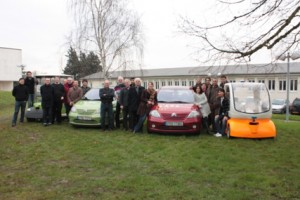
\includegraphics[width=0.7\textwidth]{Chapter1/graphics/imara.jpg}
	\caption{L'équipe-projet IMARA et quelque uns des véhicules utilisés}
	\label{fig:ch1_IMARA}
\end{figure}

\subsection{Perception de l'environnement : quels besoins pour une navigation autonome ?}
\subsubsection{Définition}
On parlera souvent dans ce manuscrit de "<perception de l'environnement\fg{}, et cette notion peut être diversement comprise. Ce premier paragraphe sera donc l'occasion d'une définition, à laquelle nous tâcherons de nous tenir par la suite. On appelle donc ici \emph{perception de l'environnement} l'action d'acquérir des informations, de quelque nature que ce soit, sur les éléments constitutifs de l'espace à proximité du porteur. Ces éléments peuvent être de nature structurelle (route, bâtiments, objets rigides, ..) ou immatérielle (position par rapport à un référentiel donné, ..), ils peuvent être constants dans le temps ou dynamiques (leur caractéristique, par exemple leur position, change avec le temps). \\
Ces informations sont très diverses par nature, et peuvent donc prendre des représentations différentes, nous en détaillerons quelques unes dans la section \ref{sec:ch2_capteurs}.

\subsubsection{Besoins de perception pour un véhicule autonome} \label{sec:ch1_besoins}
Un véhicule autonome doit, par définition, être capable de percevoir toutes les informations nécessaires à une navigation sans incident ; que ce soit vis-à-vis d'autrui (collision avec un élément de la scène) ou de son intégrité propre. Il doit par ailleurs être capable de communiquer avec son environnement dans de nombreux cas de figure, pour coordonner son action avec d'autres porteurs ou recevoir de nouvelles informations ou directives par exemple. Il doit enfin être capable de prendre des décisions et de planifier des actions de manière indépendante, ce qui implique d'acquérir préalablement suffisamment d'informations sur son environnement.\\

On peut ainsi sommairement lister quelques uns de ces besoins concrets liant un véhicule autonome et son environnement, indépendants de la représentation utilisée ou des capteurs :
\begin{itemize}
	\item perception des obstacles statiques;
	\item positionnement dans l'espace par rapport à l'environnement courant;
	\item positionnement dans l'espace par rapport à une référence absolue;
	\item détection, localisation, suivi des objets en mouvement;
	\item perception de l'espace navigable;
	\item perception de symboles porteurs de sens (panneaux, signalisation routière, ou autre).\\
\end{itemize}

Certains de ces éléments peuvent être résolus par une connaissance \textit{a priori} de la scène, et la notion de perception doit donc être comprise au sens large (acquisition d'information). On peut aisément constater que les besoins sont nombreux, bien que certains d'entre eux soient résolus depuis plusieurs années dans certaines conditions favorables. Nous n'avons pas l'ambition de répondre à tous ces besoins par la méthode présentée dans ce manuscrit, mais nous concentrerons sur quelques points particuliers.

\subsection{Buts poursuivis}
Notre travail se situe dans le domaine des véhicules autonomes, et concerne de manière plus générale tous les robots amenés à se déplacer dans un environnement dynamique. Nous souhaitons améliorer les capacités de perception des obstacles et des objets mobiles, et être capable d'estimer leurs caractéristiques dynamiques (vitesse et direction). Ces besoins sont par exemple nécessaires à l'évolution de robots dans un environnement partagé avec des humains, et constituent l'un des axes de progrès majeurs dans le domaine de la perception. Une grande proportion des algorithmes couramment utilisés pour la navigation des véhicules autonomes suppose en effet que l'environnement observé est statique, et que les éléments mobiles sont assimilables à un bruit d'observation. La connaissance de la vitesse des éléments mobiles de l'environnement autorise au contraire une planification de trajectoire plus sûre et efficace, en autorisant notamment une anticipation inaccessible aux moyens de perception restreints à un monde statique.\\

Les buts poursuivis peuvent être résumés par les quatre points suivants :
\begin{itemize}
	\item{\emph{Localisation autonome du porteur dans son environnement proche:}\\}
	La méthode proposée doit être capable d'estimer la position et le mouvement du véhicule de manière autonome, c'est à dire sans faire appel à des capteurs ou à des moyens de calcul externes.\\
	
	\item{\emph{Positionnement des obstacles statiques dans l'espace:}\\}
	La méthode proposée doit pouvoir servir de base à une détection des obstacles, ce qui suppose donc que suffisamment de points de la scène soient positionnés dans l'espace pour ne pas risquer une collision. La classification des éléments de la scène n'est cependant pas l'objet de ce travail, mais nous souhaitons obtenir les informations suffisantes pour répondre à ce besoin.\\
	
	\item {\emph{Détection des objets mobiles, de leur position et de leur vitesse:\\}}
	La méthode que nous présentons vise à détecter les objets se mouvant indépendamment du porteur, et à estimer leur position et leur vecteur vitesse. Ces informations sont utiles pour la planification de trajectoire du véhicule, et une classification postérieure de ces objets en tant qu'obstacles potentiels.\\
	
	\item{\emph{Exécution en temps réel:}\\}
	Les tâches liées à la navigation d'un véhicule autonome sont naturellement soumises à des contraintes en termes de temps de calcul. On peut se convaincre empiriquement que ces contraintes sont de l'ordre des temps caractéristiques de la dynamique du porteur (temps nécessaire pour revenir à l'immobilité notamment), que l'on résumera improprement dans la suite par \og \textit{temps réel} \fg. Cette définition n'est pas stricte dans notre cas, s'agissant de temps d'exécution qui peuvent varier selon la plate-forme de calcul notamment, mais on s'attachera à montrer que leur ordre de grandeur est adaptée à une acquisition continue d'informations visuelles, soit environ 10 à 25 images traitées par seconde.\\
\end{itemize}

\section{Organisation du manuscrit}
Le chapitre 2 est dédié à un état de l'art des systèmes de perception répondant à notre problématique. Il s'agit tout d'abord de présenter différents capteurs à même de répondre à notre problématique, ainsi que certains des algorithmes qui y sont associés dans la littérature et qui répondent à tout ou partie des besoins soulevés. Ces approches ne satisfont pas tous nos prérequis, et on proposera alors un mécanisme général visant à y répondre.\\

Le chapitre 3 sera consacré à l'acquisition d'informations à partir de capteurs d'imagerie, et au type d'information que nous souhaitons obtenir. On présentera initialement quelques uns des algorithmes présents dans l'état de l'art qui visent à exploiter des acquisitions visuelles à des fins de perception. On présentera ensuite le type d'information que nous avons souhaité utiliser, ainsi qu'une évaluation quantitative de différentes approches s'y rattachant. On présentera ensuite une implémentation très parallélisée que nous avons réalisé afin d'assurer un traitement rapide de cette étape de l'algorithme.\\

Le chapitre 4 présente une partie du processus d'inférence se basant sur les indices visuels, qui répond à une problématique d'odométrie visuelle et de reconstitution de l'environnement statique autour du porteur. On présentera une nouvelle méthode proposée pour estimer de manière rapide et robuste le mouvement, qui s'adapte aux informations visuelles ponctuelles extraites lors de l'étape précédente, et qui sera comparée à l'état de l'art. Le mécanisme proposé pour estimer la position dans l'espace d'éléments singuliers de l'environnement sera également présenté, ainsi que quelques résultats spécifiques à cette étape de l'algorithme.\\

On présente ensuite dans le chapitre 5 la détection et le suivi des objets mobiles, qui sont aussi obtenus à partir des informations extraites des acquisitions visuelles. Différentes méthodes de détection d'objets mobiles sont initialement présentées, puis nous détaillons notre proposition qui prend en compte les spécificités de notre système d'acquisition. De même, on présentera dans cette partie quelques méthodes présentes dans la littérature permettant l'estimation de la localisation et le suivi de cibles mobiles, avant de détailler l'approche que nous proposons et de commenter les résultats obtenus.\\

Le chapitre 6 est enfin consacrée à une illustration des résultats généraux de la méthode proposée, et une critique relative à son adéquation aux problématiques initiales. Nous proposerons alors quelques pistes d'amélioration des travaux existant, avant de conclure ce manuscrit.

\section{Contributions}
On propose dans ce manuscrit les contributions suivantes :
\begin{itemize}
\item Système global de perception d'un environnement dynamique, fournissant un nuage de points semi-dense suivi dans le temps. Il s'agit d'une approche globale et novatrice, qui est focalisée sur nos besoins en termes de perception des objets mobiles.\\

\item Détermination du mouvement propre de la caméra (\emph{Ego-motion}) dans un cadre adapté aux spécificités de la stéréo-vision. Il existe dans ce domaine une littérature abondante, qui n'est cependant pas toujours adaptée à nos besoins. On propose une méthode rapide et robuste qui répond très bien à notre problématique initiale.\\

\item Détection et suivi d'objets mobiles dans l'espace. On propose un système novateur, à même de détecter et d'estimer la position et la vitesse d'éléments mobiles de la scène, sans prérequis de forme ou de trajectoire, à partir d'acquisitions visuelles.
\end{itemize}

\chapter{État de l'Art}
\label{sec:ch2}
\vspace{10pt}

\minitoc
\clearpage

% % % % % % % % % % % % % % % % % % % % % % % % % % % % % % % % % % % % % % % % 
% Etat de l'Art : systèmes globaux répondant à la problématique de perception %
%	 					d'un environnement dynamique						  % 
% % % % % % % % % % % % % % % % % % % % % % % % % % % % % % % % % % % % % % % %

\section{Introduction}
On présente ici une vue d'ensemble de quelques stratégies présentes dans l'état de l'Art pour assurer à un véhicule autonome la connaissance d'un environnement dynamique. Cette problématique est largement couverte depuis quelques années, bien qu'aucune approche n'ait à notre connaissance emporté l'adhésion de tous les acteurs. Les systèmes présentés ci-dessous n'offrent ainsi pas une connaissance exhaustive de l'environnement, mais présentent chacun divers avantages, et définissent un écosystème algorithmique qui servira de référence à notre proposition. Ce sujet étant particulièrement large, toutes les techniques présentées ne sont sans doute pas couvertes dans le détail, mais on s'attachera à en faire ressortir certains des avantages et inconvénients.\\

On présente tout d'abord un ensemble de capteurs envisagés, pour répondre à notre tâche de perception de l'environnement à des fins de navigation autonome. Une observation rapide de leurs avantages et limitations nous permet ensuite d'en isoler deux types, à savoir les télémètres lasers et les solutions fondées sur la vision. Nous en présentons alors les modélisation les plus couramment utilisées, puis quelques algorithmes de l'état de l'art qui exploitent relativement directement ces modèles pour en déduire des informations utiles à la perception de l'espace et des obstacles. Nous présentons enfin quelques uns des algorithmes couramment mis en œuvre pour filtrer ces informations, et déterminer par inférence des informations qui ne sont pas directement accessibles par ces modèles. Une dernière partie est consacrée à la présentation succincte de l'approche que nous proposons, et qui sera amplement développée dans les prochaines parties. 

\section{Différents capteurs possibles} \label{sec:ch2_capteurs}
%\subsection{Capteurs actifs et passifs}
%On segmente ici les capteurs couramment utilisés en deux catégories arbitraires, qui rendent compte de la différence fondamentale entre les informations perçues : les capteurs "actifs" et %les capteurs "passifs". Dans notre segmentation, les capteurs actifs émettent une onde (acoustique ou électromagnétique) qui va permettre de "sonder" l'espace. Les capteurs que l'on appelle %"passifs" n'émettent, comme leur nom l'indique, aucune onde de quelque nature que ce soit, mais captent une onde présente dans l'environnement. Ces différences dans le mode d'action ont des %conséquences sur les informations perçues : les premiers acquièrent généralement l'espace libre dans une direction donnée, tandis que les seconds perçoivent une projection de l'environnement %selon un axe. Ces différences peuvent être directement reliées au mode de représentation de l'information choisi (insérer référence), mais cela n'est pas nécessairement le cas.

\subsection{Comparaison capteurs et besoins}
De nombreux capteurs sont envisageables à des fins de perception, aux avantages divers et parfois complémentaires. En faire une étude détaillée n'est pas l'objet de ce manuscrit, mais ce paragraphe est consacré à une brève revue de détails, afin de sélectionner les capteurs les plus à même de répondre à nos besoins. Le tableau \ref{tab:ch2_Comparaison_capteurs} offre une vue synthétique de l'adéquation des capteurs envisageables avec nos besoins, et peut être complété par les remarques suivantes :
\begin{itemize}
\item{\emph{Ultrasons:\\}}
Ces capteurs permettent une mesure de l'espace libre, mais leur très faible portée et précision limitent les informations accessibles.\\

\item{\emph{Différents télémètres laser:\\}}
On dissocie arbitrairement dans \ref{tab:ch2_Comparaison_capteurs} les télémètres laser ne comportant que quelques couches et une ouverture limitée et les télémètres de type \og Velodyne\fg{}. Ces derniers seront souvent pris comme référence par la suite, leur utilisation étant devenue courante pour des applications de cartographie ou de navigation autonome de véhicule. Ils sont constitués d'un alignement de télémètres pivotant autour d'un axe, autorisant une couverture angulaire de 360$^\circ$ par 60$^\circ$, et fournissant des centaines de milliers de points par seconde. La densité d'informations plus faible fournie par les premiers rend par exemple difficile la détection et le suivi d'objets mobiles (\cite{Wang2007, Gate2009}), ou encore la perception de l'espace navigable.\\

\item{\emph{Mono et multi-caméras:\\}}
On dissocie de même les solutions mono et multi-caméras, au vu de l'état de l'art dans leurs domaines respectifs (la perception d'un volume par une solution mono-caméra immobile est par exemple délicate). L'évaluation de la portée des solutions visuelles est délicate, selon la nature de l'information exploitée. La reconnaissance de forme ou la détection d'obstacles peuvent ainsi être typiquement réalisées à de grandes distances (\cite{Labayrade2002}), tandis que le positionnement dans l'espace est en général plus délicat. Ces performances sont par ailleurs dépendantes de la résolution du système utilisé, mais aussi de la disposition relative des caméras dans le cas de systèmes de stéréo-vision (un écartement plus important augmentant la précision de positionnement à grande distance). \\

\item{\emph{Radar:\\}}
La portée très importante (environ 200 mètres) et le faible coût des radars embarqués rend ce capteur d'ores et déjà populaire dans l'industrie automobile, mais il est pénalisé dans notre comparaison par sa faible résolution spatiale, et son ouverture angulaire limitée. De nombreuses études font cependant état de développements avancés (notamment dans la détection de piétons, voir par exemple Vivet \cite{Vivet, Vivet2013} ou Milch \cite{Milch2001}). L'ouverture angulaire limitée peut notamment être compensée par une structure tournante, comme c'est le cas pour les télémètres laser, bien que cette solution soit certainement industriellement complexe.\\

\item{\emph{Caméras de profondeur:\\}}
Les caméras dites \og 3D\fg{} (utilisant en général de la lumière structurée ou une mesure du temps de vol) n'ont pour l'instant pas réellement d'utilisation possible à l'extérieur, et ne sont donc pas envisageables pour notre application. De nouveaux dispositifs sont cependant présentés depuis quelques années, tirant profit de déformations optiques volontaires ou d'un réseau de micro-lentilles par exemple, et leur usage pourrait se généraliser dans un futur proche.\\

\item{\emph{Prix de revient:\\}}
Le prix des capteurs n'entre pas en compte dans ce tableau, qui se veut le plus général possible. Les coûts des solutions présentées diffèrent cependant grandement, que ce soit au niveau du capteur ou des traitements informatiques afférents.\\
\end{itemize}

\begin{figure} 
	\centerline{
		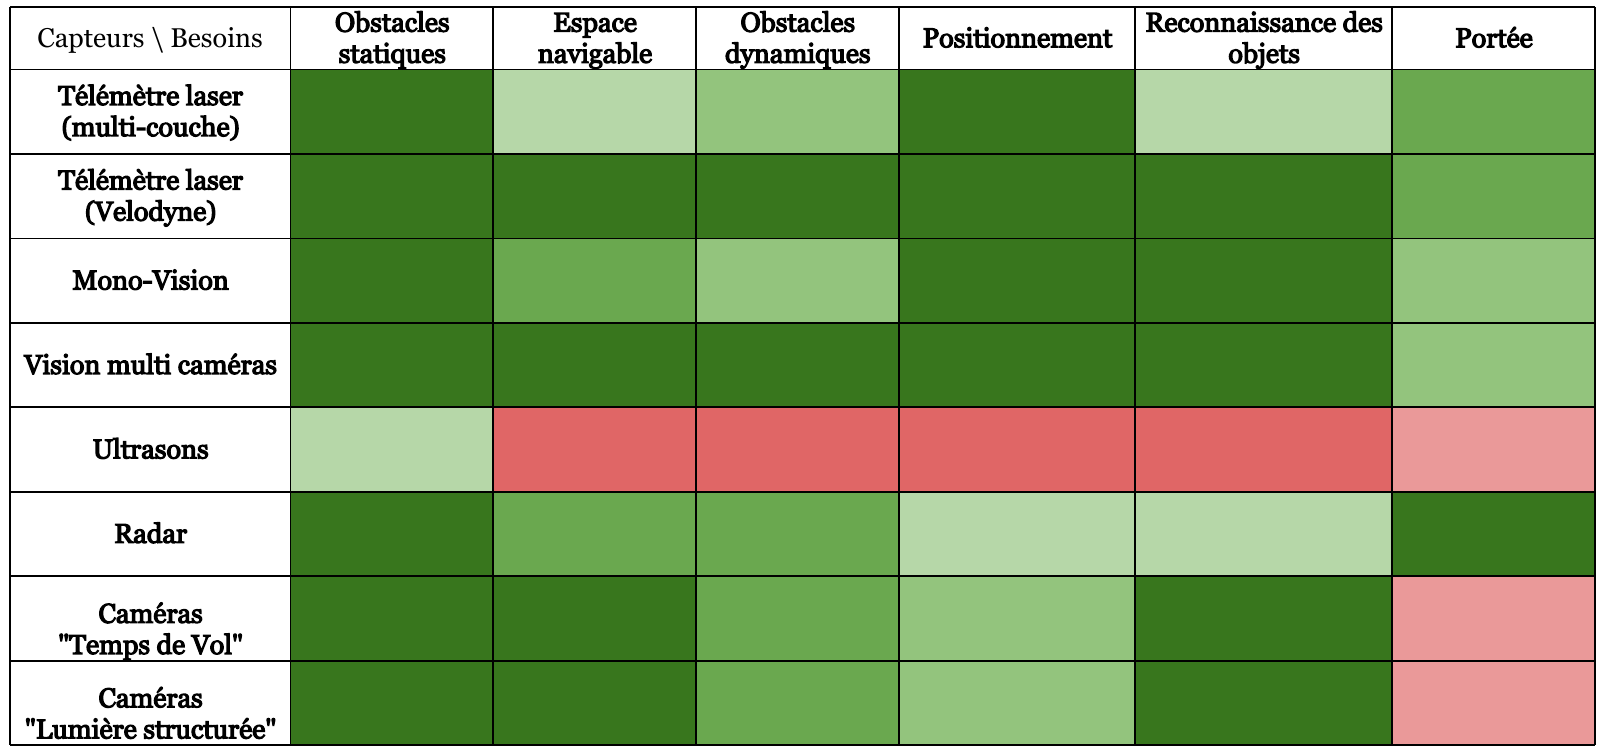
\includegraphics[width=1\textwidth]{Chapter2/graphics/sensor_needs.png}
		}
	\caption{Représentation approximative des propriétés respectives de différents types de capteurs. Les solutions présentes sont classées par leur couleur, du vert vif (point fort) au rouge vif (point faible). Une couleur moins saturée décrit une caractéristique positive ou négative moins marquée.}
	\label{tab:ch2_Comparaison_capteurs}
\end{figure}

On constate aisément au vu du tableau \ref{tab:ch2_Comparaison_capteurs} que les capteurs de type \og télémètre laser\fg{} et \og vision\fg{} sont \textit{a priori} les plus intéressants pour un tel usage. Ce constat n'est par ailleurs pas étonnant au vu de la littérature sur le sujet, qui se concentre effectivement sur ces moyens de mesure. La suite du manuscrit est donc plus particulièrement consacrée à ces deux moyens de perception.

\subsection{Modèles de capteurs}
Les informations issues d'un capteur doivent nécessairement être interprétées, pour prendre en compte son mode d'acquisition, ou les incertitudes qui y sont associées. Les capteurs perceptifs illustrent en effet différentes facettes de l'environnement, observant par exemple l'occupation selon une direction donnée ou la projection du champ électromagnétique sur un plan. Ces spécificités sont prises en compte par un modèle de capteur, description algorithmique qui permet de traduire les informations obtenues en sortie de capteur en une représentation plus abstraite. Le modèle de capteur fait donc le lien entre la mesure physique effectuée par celui-ci et les informations qui en découlent. Les modèles de capteur les plus couramment associés aux télémètres laser et à la vision sont présentés dans les sections suivantes.

\subsubsection{Télémètre laser} \label{sec:ch2_Modèle_laser}
Le télémètre laser est un capteur actif, en cela qu'il émet une onde qui \og sonde\fg{} l'espace, et qui permet de déterminer la distance au premier point d'impact (souvent par mesure du temps de vol, mais d'autres techniques, notamment fondées sur un déphasage de l'onde réfléchie ou sur l'effet Doppler sont possibles). Il fournit, de part la localisation de ce point, l'information paradoxale de l'espace libre entre le point d'émission et celui ci. Le modèle de capteur doit rendre compte de cette observation, et une approche fréquente consiste à le définir en termes de probabilité d'occupation. Celle-ci est en général négligeable entre le point d'émission et le point d'impact relevé, maximale au niveau du point d'impact, puis prolongée à son niveau maximal ou décroissante selon les besoins. La localisation du point d'impact peut être modélisée par une probabilité de présence continue, par exemple gaussienne, rendant compte de la stochastique du capteur, ou par une série de valeurs discrètes, arbitraires, rendant parfois compte de différents besoins des algorithmes en aval dans le processus de traitement. On en présente quelques exemples sur la Figure \ref{fig:ch2_laser_model}.

\begin{figure}[h]
\centering{
	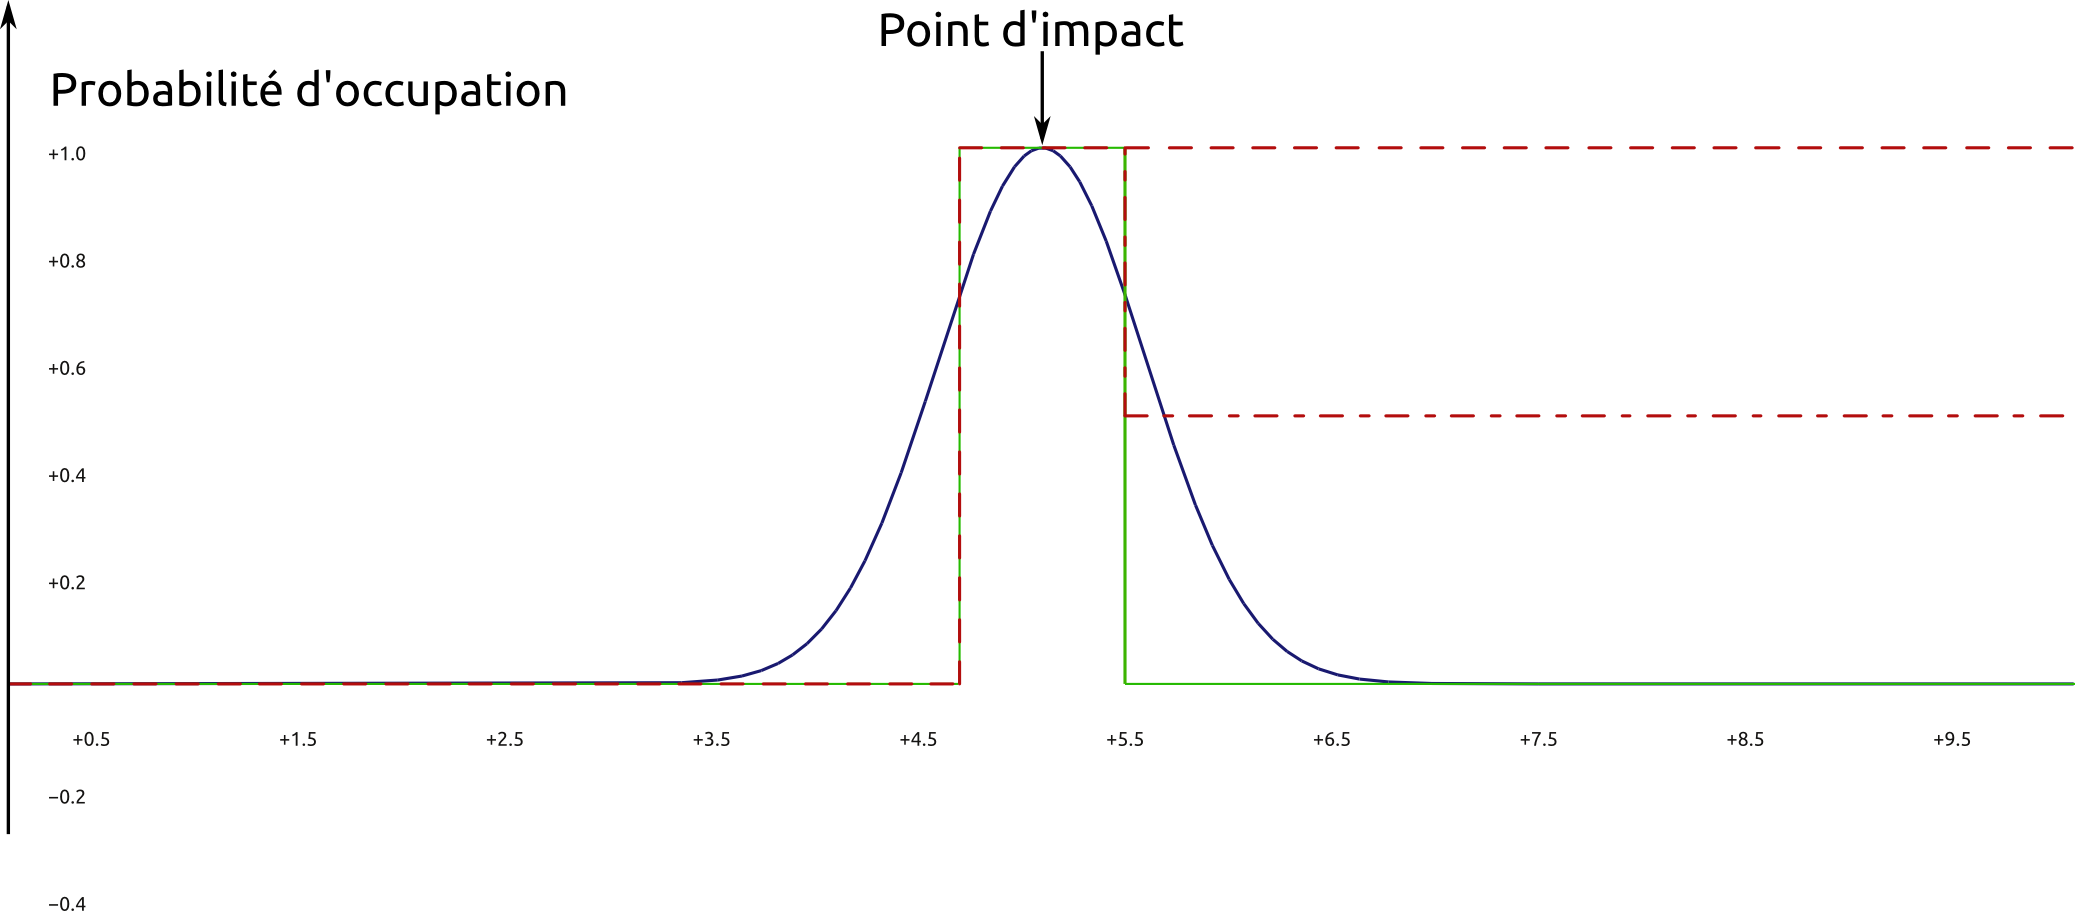
\includegraphics[width=0.9\textwidth]{Chapter2/graphics/laser_model.png}
	\caption{Exemples de différentes modélisations d'un télémètre laser, définissant la probabilité d'occupation en fonction de la distance au point d'émission et au point d'impact. La courbe bleue représente une probabilité d'occupation continue, Gaussienne. Les courbes rouges et vertes représentent un modèle discret couramment utilisés dans les représentations dites de \og grilles d'occupation\fg{}, et considèrent différemment la probabilité d'occupation de la partie occultée par le point d'impact.}
	\label{fig:ch2_laser_model}
	}
\end{figure}

La généralisation des modèles discrets dans le cas de télémètres lasers à balayage conduit souvent à une représentation dans le plan de rotation, dans laquelle la probabilité d'occupation de l'espace est échantillonnée selon une grille. On en présente un exemple dans la Figure \ref{fig:ch2_laser_grid}, dont la scène est tirée des acquisitions du projet LOVe de protection des vulnérables sur la route.

\begin{figure}[h]
	\begin{center}
		\begin{subfigure}{0.48\textwidth}
			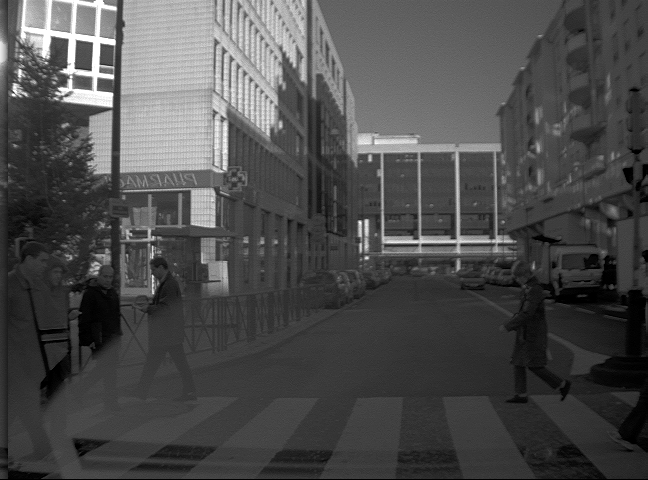
\includegraphics[width=\textwidth]{Chapter2/graphics/laser_occupancy_grid_pict.png} 
			\caption{Vue de la caméra}
		\end{subfigure}	
		~	
		\begin{subfigure}{0.48\textwidth}
			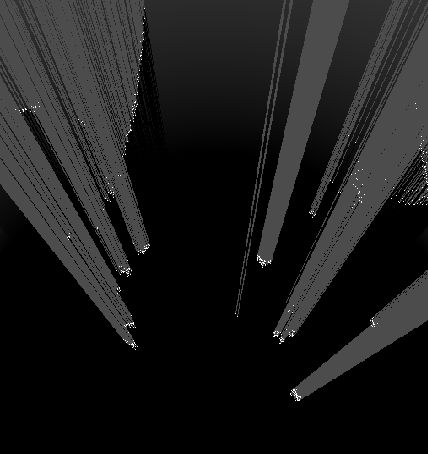
\includegraphics[width=\textwidth]{Chapter2/graphics/laser_occupancy_grid.png} 
			\caption{Application d'un modèle (\ref{fig:ch2_laser_model}) aux acquisitions d'un télémètre laser.}
		\end{subfigure}
		
		\caption{Exemple de modèle d'un télémètre laser à balayage : représentation sous la forme d'une grille d'occupation. Dans cette représentation le capteur est situé au plus bas de la grille, pointant vers le haut. La probabilité d'occupation est représentée en niveaux de gris}
		\label{fig:ch2_laser_grid}
	\end{center}
\end{figure}

On constate aisément que ce modèle autorise une détection immédiate des possibles obstacles statiques ou dynamiques, par un simple critère de proximité. Les informations extraites du capteur sont cependant minimales dans ce cas (pas de segmentation, de classification, de dynamique par exemple), et l'utilisation d'algorithmes d'inférence (voir \ref{sec:ch2_perception_spécifique} et \ref{sec:ch2_Algo_total}) est le plus souvent préférable. \\

Il n'est par ailleurs pas indispensable d'utiliser une vision probabiliste et basée sur l'occupation pour exploiter les données d'un télémètre laser. L'apparition de capteurs très denses et en trois dimensions (de type \textit{Velodyne}) a rendu possible une exploitation plus directe des mesures de points d'impact, pas nécessairement basée sur le modèle précédent.

\subsubsection{Vision}
On restreint les dispositifs de vision décrits ici à un ensemble optique accolé à un capteur d'imagerie, bien que d'autres approches soient certainement possibles sous cette dénomination. 

\paragraph{Modèle sténopé\\}
Le modèle dit \og sténopé\fg{}, du nom du dispositif optique minimal permettant l'imagerie d'une scène sur un capteur via un simple trou dans une surface opaque, est le plus couramment utilisé pour modéliser le processus d'acquisition d'images à partir d'une scène en trois dimensions. On considère dans l'équation \ref{eq:ch2_modèle_sténopé} les coordonnées ${u,v}$ dans le plan image, et ${X,Y,Z}$ dans le repère monde. L'orientation de ces repères est la suivante :
\begin{itemize}
	\item{} $u$ et $x$ sont parallèles et orientés dans le même sens, de même que $v$ et $y$.\\
	\item{} $z$ complète $x$ et $y$ pour en faire un repère orthonormé, et est orienté vers le fond de la scène.\\
	\item{}	$f$ est la focale de l'optique, c'est à dire la distance entre le plan optique et le plan de convergence d'un front d'onde provenant d'une source située à l'infini. L'équation suivante s'obtient aisément en considérant un système optique simplifié (une seule lentille de focale connue) et des observations géométriques.\\
\end{itemize}

Les coordonnées $u_0$ et $v_0$ décrivent les distances dans le plan image entre l'origine du repère, qui peut être choisie arbitrairement (par exemple en haut à gauche de l'image dans le cas d'un adressage informatique), et l'intersection de l'axe optique et du plan image. Une représentation de ce modèle est visible sur la figure \ref{fig:ch2_modèle_sténopé}.

\begin{figure}[h]
	\begin{center}
		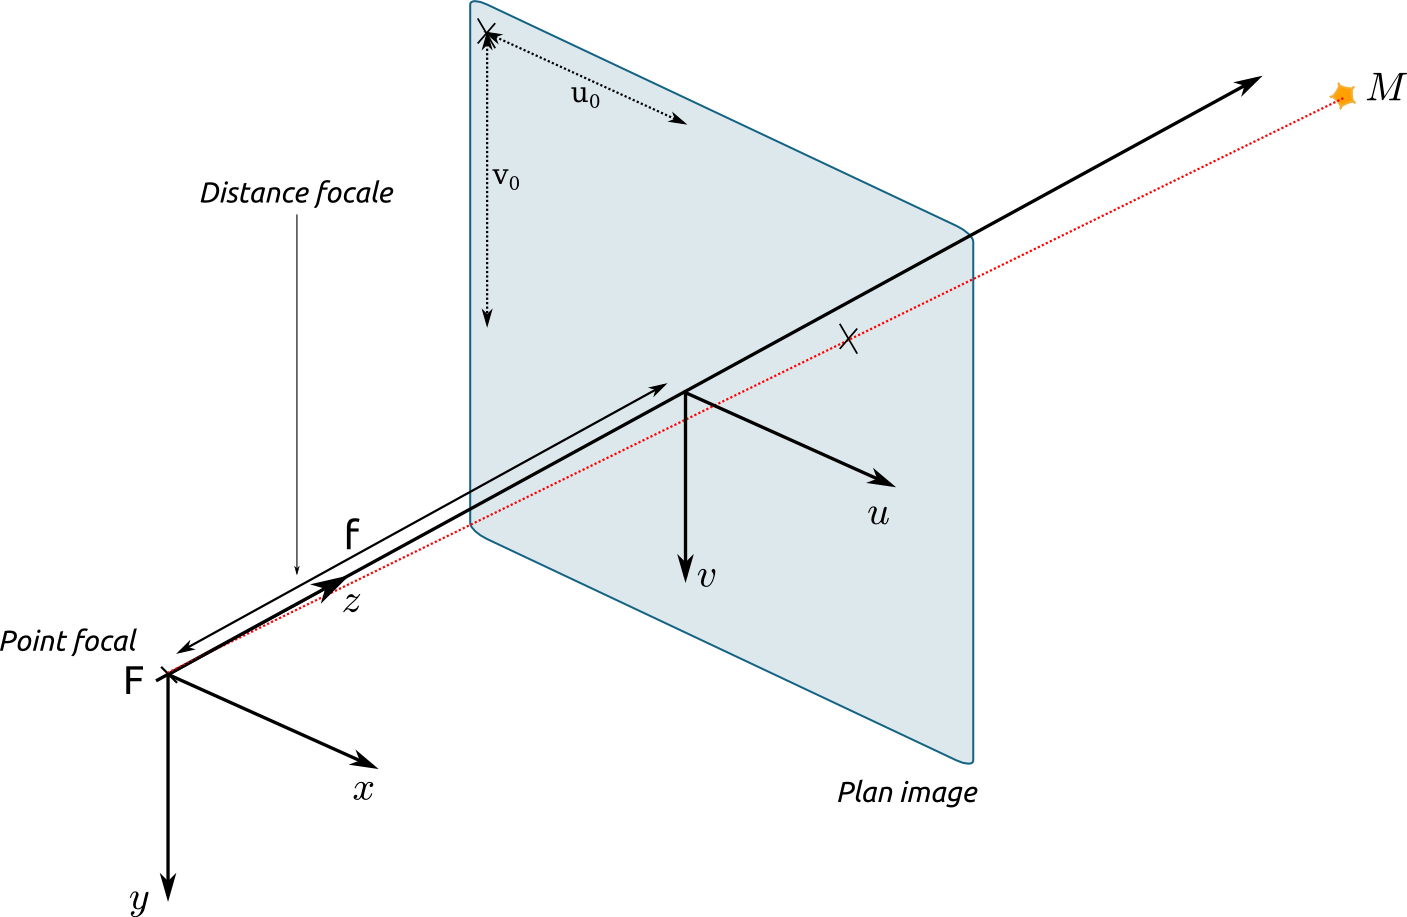
\includegraphics[width=0.7\textwidth]{Chapter2/graphics/pinhole_model.png}
		\caption{Illustration du modèle sténopé}
		\label{fig:ch2_modèle_sténopé}
	\end{center}
\end{figure}

\begin{equation} \label{eq:ch2_modèle_sténopé}
	\begin{array}{|c}
		u\\
		v\\
	\end{array}
= 
	\begin{array}{|c}
		u_0 + f \cdot \frac{X}{Z}\\
		v_0 + f \cdot \frac{Y}{Z}\\
	\end{array}
\end{equation}

La transformation décrite n'est pas bijective, c'est à dire que la connaissance de la position dans l'espace d'un objet permet d'en déduire sa projection sur le plan image, mais que le processus inverse n'est pas déterminé. La position dans l'espace d'un point présent dans le plan image est déterminée à un degré de liberté près, ce qui se matérialise par une ligne dans l'espace sur laquelle ce point peut se trouver.\\

Ce modèle est par ailleurs une représentation simplifiée du processus d'imagerie, mais il reste très largement utilisé et souvent suffisamment performant. L'approximation d'une projection parfaite de l'image sur un plan n'est pas respectée pour les caméras dotées d'un très grand angle de prise de vue, et d'autres modèles peuvent alors être introduits (projection sur une sphère notamment), qui ne seront pas détaillés ici. Il est par ailleurs possible de modéliser les erreurs optiques distordant l'image projetée par des polynômes simplifiés, décrivant la projection d'une droite du repère monde dans le plan image. Cette correction est souvent relativement grossière, les applications à base de vision dans le domaine de la robotique étant empiriquement peu sensibles aux erreurs de rectilinéarité.

\paragraph{Stéréo-vision\\} \label{sec:ch2_Modèle Stéréovision}
Un dispositif de stéréo-vision combine deux caméras dont les positions et orientations relatives sont connues. Le modèle \og sténopé\fg{} peut à nouveau être mis à profit dans ce cas de figure, et la connaissance de la position d'un élément de l'espace dans deux plans image distincts permet cette fois de définir un modèle global bijectif. On peut en effet reprendre les calculs \ref{eq:ch2_modèle_sténopé}, et les développer dans le cas d'une projection sur les plans image $P_1$ et $P_2$, dont on connaît les positions relatives. Il faut dans ce cas tenir compte de l'origine distincte des deux repères utilisés pour la projection. Dans un cas quelconque, les repères des deux caméras diffèrent d'une transformation rigide, composée d'une rotation et d'une translation, comme illustré dans la figure \ref{fig:ch2_stereo_quelconque}. \\
On a vu que l'antécédent d'un point du plan image par l'équation du modèle sténopé (\ref{eq:ch2_modèle_sténopé}) était une droite. On définit dans ce cas la droite épipolaire liée au point $M$ comme l'image par le capteur $C_2$ de la droite antécédente de la projection du point $M$ sur le capteur $C_1$. Cette droite est importante lors de la recherche dans le plan $P_2$ de la projection du point $M$, lorsque celle-ci est déjà connue dans le plan $P_1$. Le point $M$ imagé par le capteur $C_2$ peut alors être recherché le long de la droite épipolaire uniquement.\\

\begin{figure}[h]
		\begin{center}
			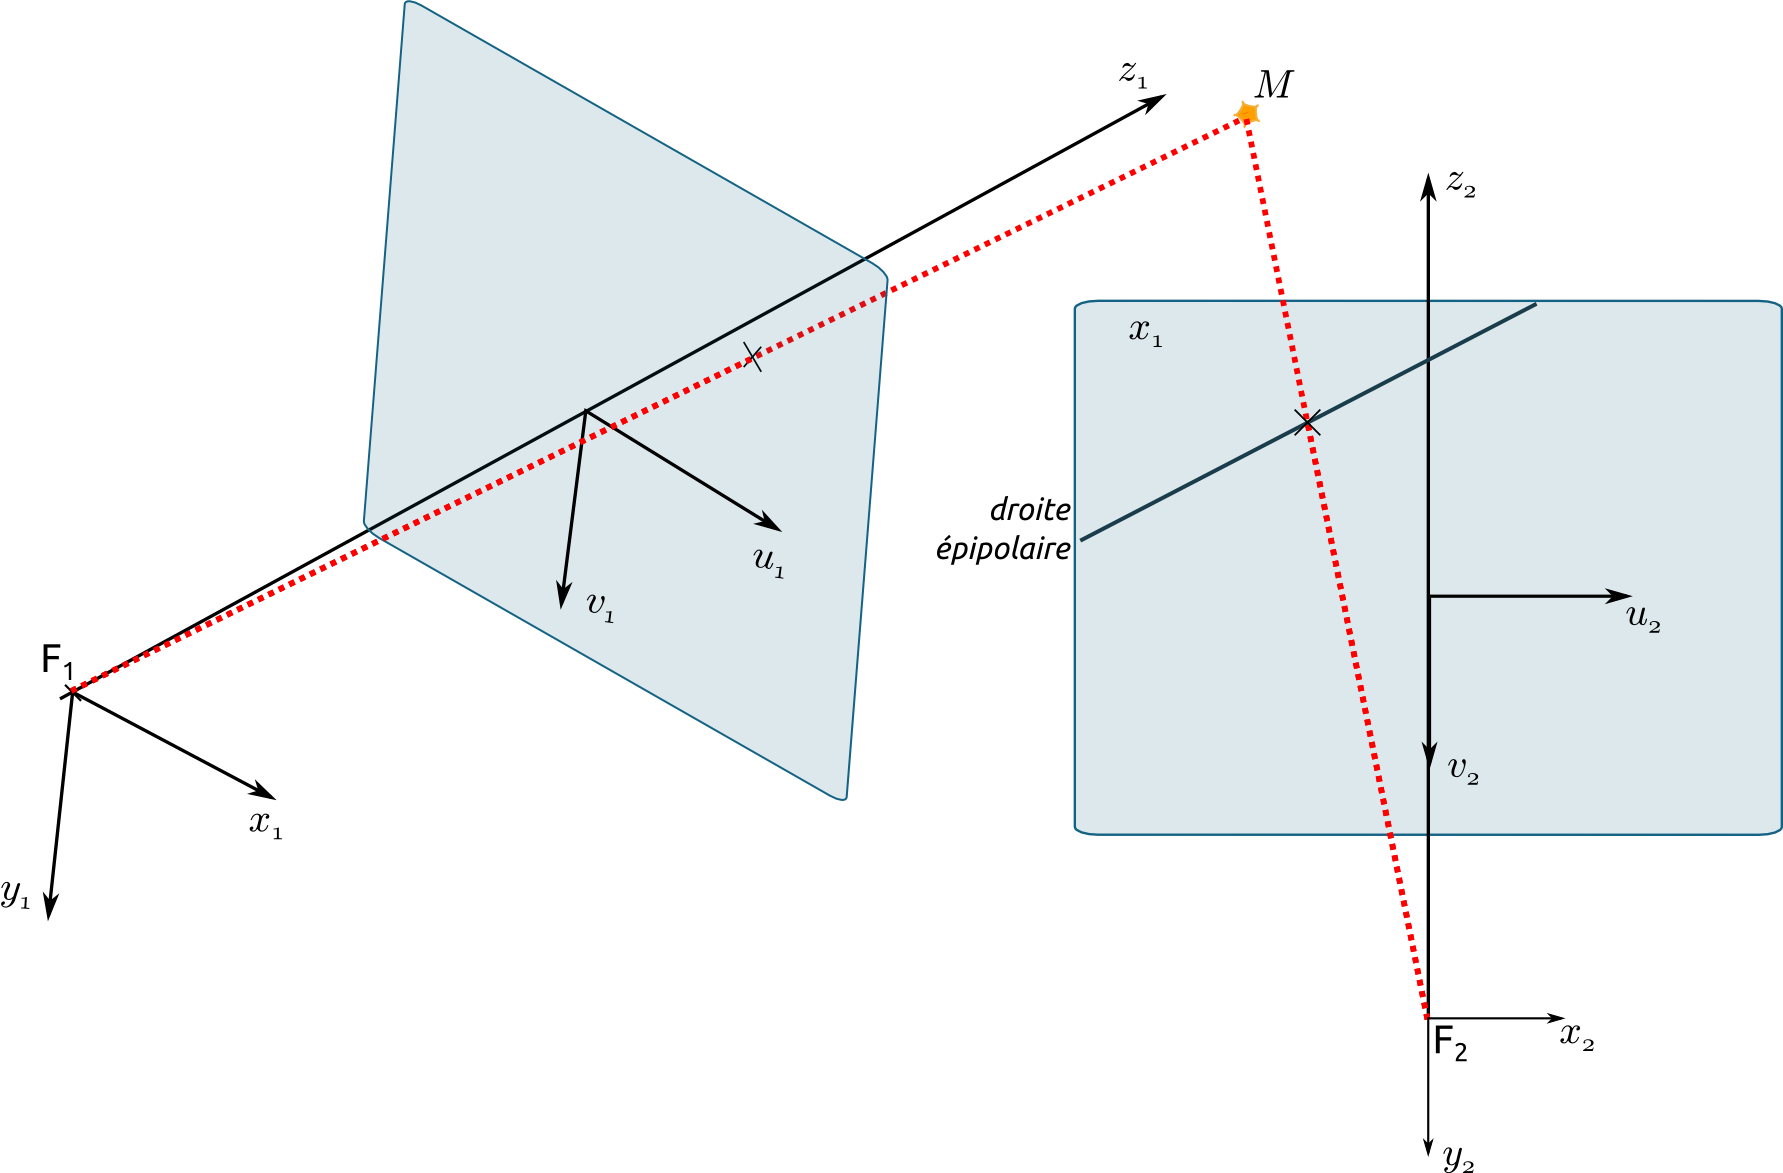
\includegraphics[width=0.7\textwidth]{Chapter2/graphics/stereo_model_random.png}
			\caption{Système de stéréo-vision quelconque. Les angles sont exagérés par rapport à un système typique, pour les besoins de l'illustration.}
			\label{fig:ch2_stereo_quelconque}
		\end{center}
\end{figure}

L'utilisation de l'équation \ref{eq:ch2_modèle_sténopé} appliquée à chacune des caméras, et exprimée dans un même repère, nécessite alors l'usage d'une matrice de rotation et d'un vecteur de translation. Il est cependant possible de grandement simplifier les calculs par une opération dite de \og rectification\fg{}, qui permet de se placer dans le cas où les repères des deux plan image sont reliés par une unique opération de translation. Cette correction peut être effectuée sur un système de stéréo-vision dont les caméras sont approximativement alignées, au prix d'une réduction de la surface imagée par chaque caméra. Elle implique de déterminer préalablement les paramètres géométriques reliant les deux systèmes de coordonnées. Afin de simplifier les calculs de disparité, c'est à dire de la différence de position d'un même élément image dans les deux plan image, il est courant de corriger les images afin de se ramener à une translation le long du vecteur $\arrowvert{u}$ entre les deux plan image.

\begin{figure}[h]
	\begin{center}
		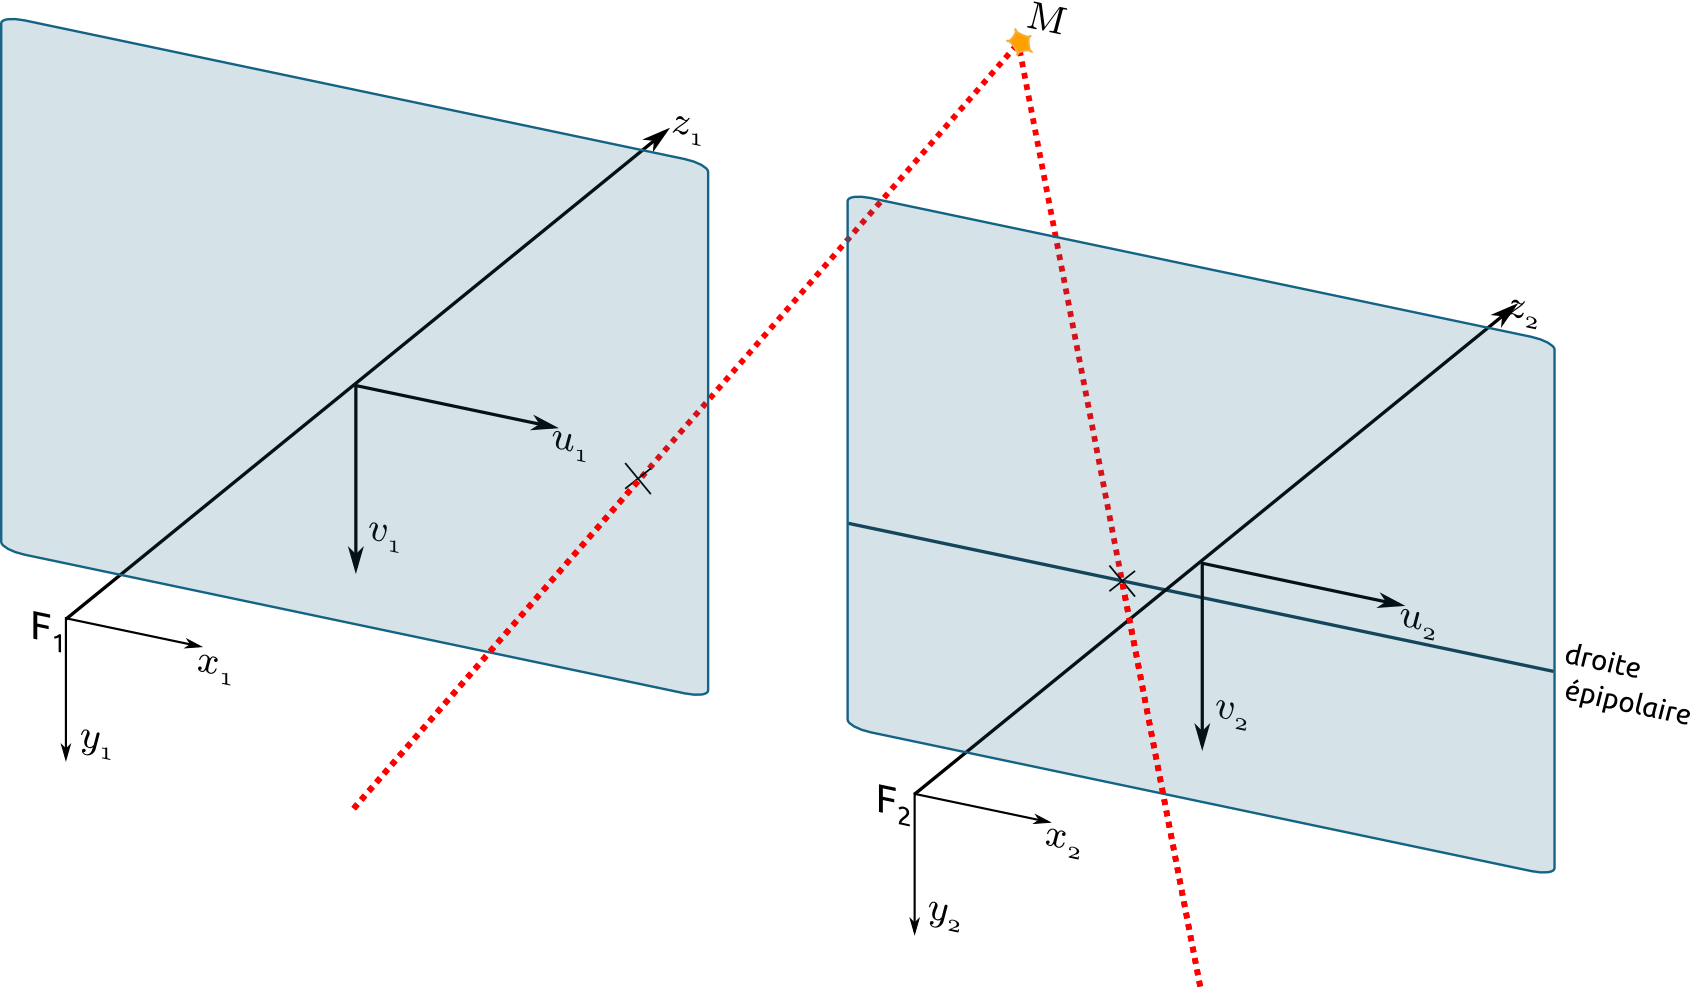
\includegraphics[width=0.7\textwidth]{Chapter2/graphics/stereo_model_rectified.png}
		\caption{Système de stéréo-vision rectifié}
		\label{fig:ch2_stereo_rectifié}
	\end{center}
\end{figure}

Les équations décrivant la relation entre le référentiel \og monde\fg{} et les deux plan image peuvent alors s'écrire relativement simplement (équation \ref{eq:ch2_modèle_stéréo}).

\begin{align} \label{eq:ch2_modèle_stéréo} 
	\begin{split}
		\begin{array}{|c}
		u_1\\
		v_1\\
		\end{array}	
		&=
		\begin{array}{|c}
		{u_0}_1 + f_1 \cdot \frac{X - X_1}{Z - Z_1}\\
		{v_0}_1 + f_1 \cdot \frac{Y - Y_1}{Z - Z_1}\\
		\end{array}	\\ \\
		\begin{array}{|c}
			u_2\\
			v_2\\
		\end{array}
		&= 
		\begin{array}{|c}
			{u_0}_2 + f_2 \cdot \frac{X - X_2}{Z - Z_2}\\
			{v_0}_2 + f_2 \cdot \frac{Y - Y_2}{Z - Z_2}\\
		\end{array}
	\end{split}
\end{align}

Si l'on suppose maintenant que l'origine de chacun des repères image est définie de la même façon (${u_0}_1 = {u_0}_2$, ${v_0}_1 = {v_0}_2$), et que les focales des systèmes optiques sont les mêmes ($f_1 = f_2$), on peut utiliser la rectification pour simplifier l'équation \ref{eq:ch2_modèle_stéréo}. Les repères des deux caméras peuvent être représentés par un unique repère, dans lequel $Y_1 = Y_2 = Y_C$, $Z_1 = Z_2 = Z_C$, et $X_2 = X_1 + b$ (avec $b$ l'écartement entre les deux centres optiques des caméras $C_1$ et $C_2$, nommée \textit{baseline} dans la littérature anglophone). On obtient finalement les équations bien connues d'un système de stéréo-vision, reliant le repère monde au repère unifié des deux caméras (équation \ref{eq:ch2_stereo_equations}).

\begin{align} \label{eq:ch2_stereo_equations}
	\begin{split}
		z& = \frac{f * b}{d}	\\
		y& = \frac{(v - v_0) * z} {f}	\\
		x& = \frac{(u - u_0) * z} {f}
	\end{split}
\end{align}

Ce calcul peut alors être exploité pour connaître la position de tout ou partie des éléments imagés, exception faite des éléments visibles sur une seule des deux caméras. Dans la perspective d'une détection d'obstacles, on peut alors choisir de se concentrer sur les informations présentes dans la carte de disparité (homogène à une ligne de vue dans la direction de chacun des pixels considérés), comme illustré sur la figure \ref{fig:ch2_disparity_map}. Il est également possible de se fonctionner directement dans le repère \og monde\fg{}, à partir des coordonnées (x, y, z).\\

\begin{figure}[h]
	\begin{center}
		\begin{subfigure}{0.48\textwidth}
			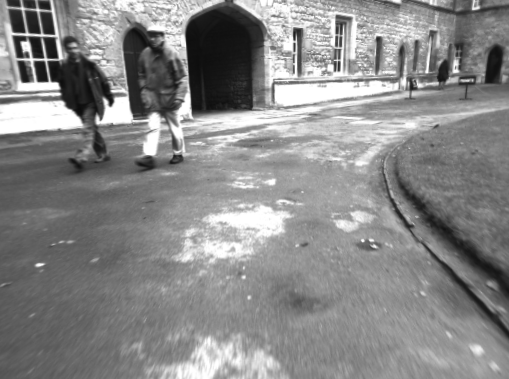
\includegraphics[width=\textwidth]{Chapter3/graphics/OF_Farneback_RAW.png} 
			\caption{Une des deux images sources.}
		\end{subfigure}	
		~	
		\begin{subfigure}{0.48\textwidth}
			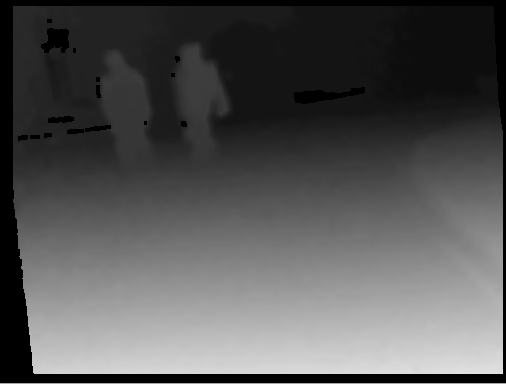
\includegraphics[width=\textwidth]{Chapter2/graphics/dense_disparity.png} 
			\caption{Carte de disparité.}
		\end{subfigure}
		
		\caption{Exemple de carte de disparité obtenue par la méthode ELAS (Geiger,\cite{Geiger}). La disparité est représentée par une valeur en niveaux de gris}	
		 \label{fig:ch2_disparity_map}
	\end{center}
\end{figure}

Une limite de ce modèle réside dans le bruit associé à la localisation dans l'espace, fortement anisotrope pour une distance grande devant la \textit{baseline} (voir par exemple \cite{Blostein1987}, \cite{Demirdjian2001} ou \cite{Sibley2007}, \cite{Lenz2011}). Ce bruit peut être modélisé, si l'on néglige les erreurs de calibration optique et géométrique du dispositif, par les équations suivantes : 

\begin{itemize}
	\item La position d'un même point est déterminé sur les deux plans image avec la dispersion $\delta$, que l'on suppose isotrope dans le plan image. Cette dispersion peut être liée à l'échantillonnage de l'image sur ses deux axes, mais aussi à la procédure d'identification du point, par exemple lors d'une corrélation (la largeur du pic de corrélation n'est pas nulle, et introduit donc une erreur possible de positionnement).\\
	
	\item Le calcul de l'erreur de positionnement d'un point dans l'espace consécutif à une erreur de positionnement $\delta$ dans le plan image (pour un dispositif rectifié) s'écrit :
	\begin{align}
		\begin{split}
			\delta_z &= \frac{\delta \cdot f \cdot b}{d^2} \\
			\delta_x &= \frac{\delta \cdot (u - u_0) \cdot b}{d^2} \\
			\delta_y &= \frac{\delta \cdot (v - v_0) \cdot b}{d^2} \\
		\end{split}
	\end{align}
\end{itemize}

On constate aisément que l'erreur de positionnement est dépendante de la position du point par rapport à l'axe optique, et de l'éloignement du point par rapport au plan image. Ce bruit de changement de repère est par exemple illustré par la Figure \ref{fig:bruit_disparité}, tirée de la publication de Lenz et al \cite{Lenz2011}.

\begin{figure}
	\centering{
		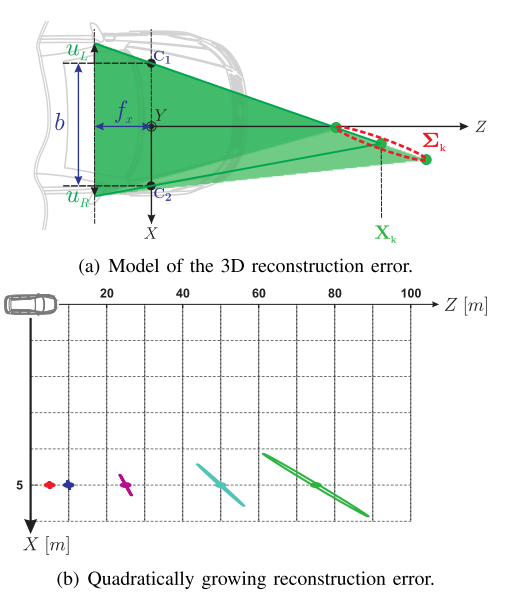
\includegraphics[width=0.6\textwidth]{Chapter2/graphics/noise_disparity.png}
	}
	\caption{Illustration du bruit lors du changement de repère (image -> monde), tirée de \cite{Lenz2011}}
	\label{fig:bruit_disparité}
\end{figure}

\subsection{Capteur retenu dans le cadre de la méthode proposée} \label{sec:ch2_capteur_retenu}
Nous avons choisi de nous concentrer sur l'usage d'un dispositif de stéréo-vision, bien qu'un travail préliminaire en début de thèse ait été consacré à l'usage d'un télémètre laser (voir \ref{sec:ch5_Bayésien_2D}). Ce travail préliminaire a mis en avant la difficulté d'estimation de la vitesse des éléments de la scène avec un tel capteur, et nous avons pensé que l'usage de la vision était intéressant dans ce cadre, parallèlement à d'autres avantages propres (coût de mise en œuvre, usages variés -reconnaissance de personnes, de panneaux, etc..-). L'état de l'art dans le domaine de l'association dans le temps d'éléments visuels d'une scène est en effet important, ce qui autorise alors une estimation de la vitesse relative des éléments de la scène. Cette tâche est toujours délicate avec un capteur télémétrique, et demeure une problématique de recherche actuelle.
La nécessité d'avoir deux caméras peut être un handicap par rapport aux dispositifs mono-caméra, qui est souvent mis en avant dans la littérature. Les informations disponibles sont cependant plus importantes dans ce cadre, et comme nous l'avons montré dans ce travail, autorisent des usages nouveaux. La reconstruction d'environnement dense, la détection et le suivi d'objets mobiles, la perception d'un environnement en trois dimensions par un dispositif à l'arrêt sont autant de tâches accessibles à un système stéréo-vision, et plus difficilement appréhendable par les systèmes mono-caméra. 

\section{Différents types de représentations}
Indépendamment des capteurs utilisés, les informations collectées par le capteur ou par le mécanisme d'accumulation mis en place peuvent utiliser différentes représentations. Celles-ci sont liées aux algorithmes d'inférence ou de fusion de données utilisés, et peuvent avoir des avantages spécifiques. Elles ne sont pas nécessairement exclusives, plusieurs représentations étant parfois utilisées parallèlement.

\subsection{Représentation des attributs physiques}
Les caractéristiques physiques déterminées par le capteur, ou par inférence, peuvent être soumises à différentes représentations. On peut mettre en avant deux approches, très différentes par leur principe et par leurs conséquences sur l'accumulation de l'information. De manière arbitraire, on classe les approches suivantes selon l'élément clef du référencement des observations : l'espace, ou le temps. On se concentre dans le premier cas sur une information, dont on veut connaître la valeur en tout point de l'espace, par exemple la probabilité d'occupation. Dans le second cas, on se concentre sur l'évolution dans le temps de points de mesure, par exemple la position d'un objet initialement détecté.\\

\subsubsection{Représentation dense dans l'espace}
On peut tout d'abord présenter les représentations liées à la connaissance de l'espace, dans lesquelles les informations sont cumulées de part leur position. On cherche ici à connaître l'ensemble du champ de valeur autour du véhicule, qu'il s'agisse de l'occupation, de la vitesse, ou d'autres caractéristiques (navigabilité, etc). Les informations sont dans ce cas placées sur une \og grille\fg{}, échantillonnage régulier ou non de l'espace, tel qu'initialement proposé par Moravec et Elfes (\cite{Moravec1985, Elfes1989a,Elfes1987}). Une représentation d'une telle grille d'occupation, telle qu'obtenue par Moravec et Elfes dans leur publication initiale, et visible sur la figure \ref{fig:ch2_grille_occupation}. \\

Les lois de mise à jour d'une telle représentation peuvent prendre des formes différentes, et intègrent souvent une inférence Bayésienne. Plus récemment, la théorie des croyances, introduite par Dempster et Shafer (\cite{Dempster1967}), est également fréquemment utilisée (voir par exemple Moras \textit{et al.}\cite{Moras2011a}). Cette représentation a l'avantage de la densité dans l'espace, et est souvent très appropriée aux moyens de calculs informatiques, de part sa régularité. \\
On suppose cependant le plus souvent dans cette représentation que le système peut être modélisé par une chaîne de Markov d'ordre 1, c'est-à-dire que toutes les informations permettant de prédire l'état futur sont contenues dans l'observation précédente. La considération d'ordres supérieurs augmente en effet très rapidement les coûts calculatoires dans le cas d'une représentation \og dense\fg{} comme celle-ci, au point d'être en pratique impossible. L'appariement des mesures d'une itération sur l'autre n'est en revanche pas nécessaire dans cette approche, ce qui en fait une représentation couramment utilisée pour les capteurs pour lesquels cette étape est délicate (télémètres lasers par exemple). 

\begin{figure}
	\centering{
		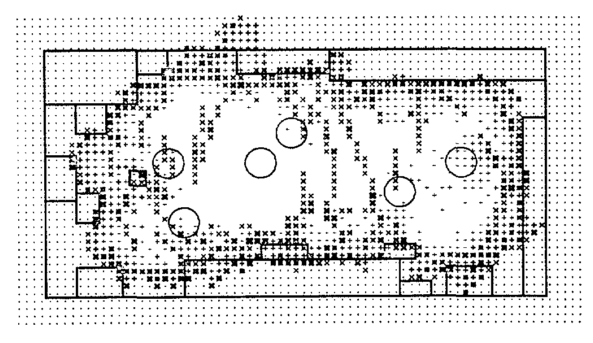
\includegraphics[width=0.6\textwidth]{Chapter2/graphics/moravec_elfes_occupancy_grid.png}
	}
	\caption{Grille d'occupation obtenue par un capteur sonar, tirée de la publication séminale de Moravec et Elfes \cite{Moravec1985}. Les positions du capteur lors des différentes acquisitions sont représentées par des cercles. La probabilité d'occupation est illustrée par le symbole \og X\fg{}, selon sa largeur. Une probabilité d'occupation inconnue est représentée par le symbole \og .\fg{}.}
	\label{fig:ch2_grille_occupation}
\end{figure}

\subsubsection{Représentation dense dans le temps}
Par opposition à l'approche spatiale basée sur des grilles présentées précédemment, il est possible d'adopter une approche complémentaire, qui prend en compte les observations concernant une même entité au fil du temps. Cette approche suppose un appariement des observations, par exemple sur des critères spatiaux ou visuels. Cette étape peut être délicate, mais divers cadres probabilistes existent (voir par exemple la section \ref{sec:ch5_GMPHD}). Il est possible dans cette représentation d'envisager une modélisation prenant un important historique de mesures en compte, même si cette possibilité est rarement exploitée, du fait de coûts calculatoires rapidement rédhibitoires. La faible densité des informations (limitées aux observations) peut rendre cette solution intéressante dans un cas où les capacités de calcul sont limitées. \\
Un exemple d'une telle représentation est visible sur la figure \ref{fig:ch2_suivi_temps_epars}, tirée des travaux de Schindler et al. \cite{Schindler2010} à des fins illustratives uniquement. Les observations sont éparses dans l'espace, et correspondent à des candidats possibles pour une détection et un suivi de piétons (\textit{a}). Les observations sont associées dans le temps (\textit{b}), et génèrent alors une trajectoire dense dans le temps (chaque pas de temps est associé à une position dans l'espace). Plusieurs cibles peuvent être suivies simultanément, la connaissance d'une trajectoire passée permettant d'envisager plus précisément les associations futures (\textit{c} et \textit{d})

\begin{figure}
	\centering{
		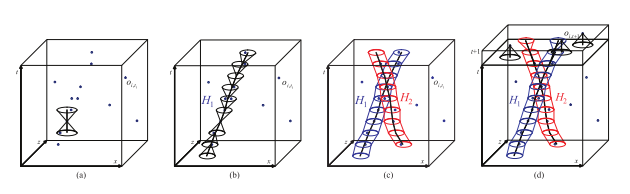
\includegraphics[width=0.8\textwidth]{Chapter2/graphics/schindler_pedestrian_tracking.png}
	}
	\caption{Suivi de cibles dans le temps, à partir d'observations éparses dans l'espace. Illustration tirée de \cite{Schindler2010}}
	\label{fig:ch2_suivi_temps_epars}
\end{figure}

\subsection{Représentation ensembliste, par connexité}
Il est parfois bénéfique d'ajouter aux connaissances précédemment décrites celle de liens existant entre plusieurs entités observées. Ces liens peuvent, par exemple, être temporels (le même objet est visible sur plusieurs acquisitions, à des positions potentiellement différentes) ou spatiaux (acquisitions liées par leur proximité géographique). Ces liens décrivent une topologie particulière, un graphe, dont l'exploitation est souvent primordiale dans un contexte de rapidité d'exécution et de robustesse.\\
De nombreuses publications récentes tirent profit de ces organisations topologiques, que ce soit pour exploiter les fermetures de boucles (passages répétés dans le même environnement, source d'information pour un système SLAM, voir par exemple FrameSLAM \cite{Konolige2008} - Slam visuel par optimisation - , GraphSLAM \cite{Thrun2006a} - SLAM laser à grande échelle-, Strasdat \cite{Strasdat} - pour une extension d'un SLAM visuel à base d'EKF prenant en compte les fermetures de boucles -) ; ou pour accélérer la localisation dans un environnement préalablement cartographié (voir par exemple Meilland \cite{Meilland2011} pour un rapprochement d'une observation avec des sphères d'images et de cartes de profondeur, ou Sinha \cite{Sinha2012} pour une relocalisation au sein d'un environnement modélisé à partir de \og Structure From Motion\fg{} (SFM)). Une illustration de la représentation utilisée par FrameSLAM est présente sur la figure \ref{fig:ch2_connexité}.

\begin{figure}
	\centering{
		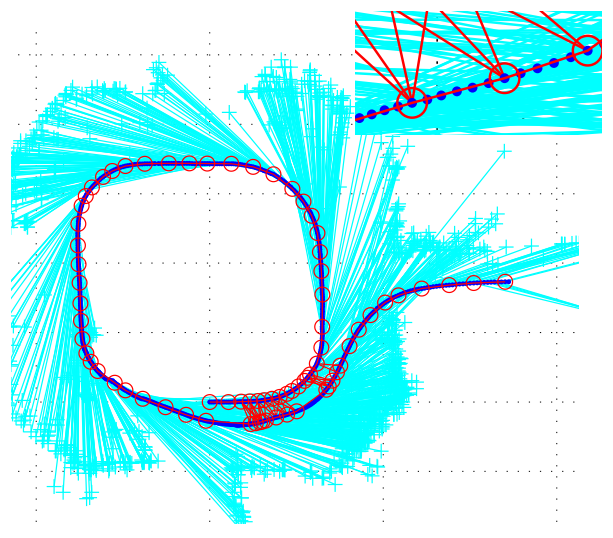
\includegraphics[scale=0.5]{Chapter2/graphics/frame_slam.png}
		\caption{Exemple de représentation par connexité, tirée de l'article \cite{Konolige2008} présentant FrameSLAM (Konolige et al.). Les acquisitions se font le long de la trajectoire bleu foncé, chaque acquisition étant représentée par un cercle rouge. Les segments rouges lient les acquisitions présentant des éléments en commun malgré une grande séparation temporelle.}
		\label{fig:ch2_connexité}
	}
\end{figure}

\subsection{Représentation paramétrique : introduction d'un \textit{prior}} \label{sec:ch2_représentation_paramétrique} % Paramétrique ?
L'environnement dans lequel les moyens de mesure évoluent est souvent connu, et il peut être intéressant d'en tirer profit dans la représentation qui en est faite. Cette notion s'appelle un \og prior\fg{} dans le domaine des probabilités, a savoir l'exploitation d'une connaissance a priori de certains éléments auxquels des propriétés peuvent être associés une fois leur identification effectuée. Ces propriétés connues peuvent concerner plusieurs domaines, par exemple (et pas exclusivement) : 
\begin{itemize}
	\item {\textit{Les caractéristiques spatiales : }\\}
	l'environnement rencontré peut souvent être décrit par des primitives (lignes droites, courbes paramétrées, etc..), ou par un jeu de formes de base. Ce \textit{prior} peut notamment améliorer la précision et la robustesse du positionnement et de la cartographie, ou simplifier son enregistrement. Moutarlier et Chatila proposent ainsi l'utilisation de lignes droites en deux dimensions pour représenter un environnement plan, et en déduire le mouvement d'un robot à partir d'acquisitions d'un télémètre laser (\cite{Moutarlier1990a}). Cette représentation peut simplifier l'accumulation des connaissances, en réduisant les degrés de liberté des informations conservées, mais aussi rendre un algorithme plus robuste au bruit. Le processus d'association des mesures à un modèle peut en effet tolérer des erreurs, tandis que la précision du modèle obtenu est ensuite fonction du nombre de points de mesure mis à contribution. On peut de ce fait obtenir les paramètres relativement précis d'un modèle à partir d'acquisitions bruitées. L'appariement des acquisitions successives est également rendu plus facile par cette modélisation, que ce soit pour estimer le mouvement du véhicule, ou pour estimer le mouvement d'éléments mobiles (voir la publication fondatrice de Wang (\cite{Wang2004}). \\
	Grandjean et Robert de Saint-Vincent proposent un principe similaire en trois dimensions (\cite{Grandjean1989}), pour mieux exploiter les acquisitions stéréoscopiques. Celles-ci présentent en effet un bruit de mesure très marqué, que la modélisation de l'environnement par des plans successifs en trois dimensions permet de mitiger. De même, Nashashibi et Devy (\cite{Nashashibi1993}) proposent de segmenter les cartes de profondeur issues d'acquisitions stéréoscopiques en différents plans. Le mouvement du véhicule peut alors être inféré par l'étude de la correspondance entre ces plans, et le modèle de la scène peut être incrémentalement augmenté. Bak (\cite{Bak2011}) propose notamment d'exploiter un principe similaire, mais à partir de prises de vues monoculaires, dans une méthode appelée \textit{C-Vélocité}.\\
	Dans un autre domaine, les lignes de marquages sont également couramment modélisées par un \textit{prior} dans la littérature, notamment grâce à une courbe clothoïde (\cite{Vacek2006}).\\
	
	\item {\textit{Les caractéristiques dynamiques : \\}}
	les déplacements possibles de l'ensemble des éléments de l'environnement peuvent être connus, et apportent alors une information significative. De même que précédemment, ceci peut permettre d'améliorer la précision et la robustesse des mesures en exploitant les contraintes sur les mouvements observables. Ces limites dans les mouvements attendus peuvent également avoir des conséquences sur les algorithmes de prédiction du déplacement, certains algorithmes de planification du mouvement se situant explicitement dans le domaine des trajectoires possibles. La recherche de trajectoires optimales est alors simplifiée du fait de la restriction de l'espace des trajectoires envisagées (\cite{Klancar2010}).\\
	
	\item{\textit{Les caractéristiques visuelles:}\\}
	la présence d'éléments dont l'apparence est connue permet parfois d'exploiter là encore un prior concernant ses propriétés attendues. De fait, la reconnaissance visuelle est l'objet de nombreux travaux dans le domaine de l'algorithmie, et atteint depuis plusieurs années des taux de détections remarquables pour certains éléments connus. La reconnaissance des piétons, des feux, des panneaux ou des pannonceaux (pour rester dans le domaine des transports) est ainsi très présente dans l'état de l'art. De nombreux exemples existent dans la littérature, les méthodes utilisées pour exploiter ce prior pouvant varier entre un ajustement de modèle ou une signature complexe déterminée par apprentissage statistique. De Charette et Nashashibi (\cite{Charette2009}) proposent par exemple une procédure de reconnaissance des feux tricolores, en exploitant la corrélation  visuelle entre un modèle et une détection préalable de points lumineux. Schindler \textit{et al.} (\cite{Schindler2010}) proposent le couplage d'un mécanisme de SLAM visuel et d'une détection de piétons par apprentissage ; afin d'améliorer celle-ci par inférence dans le temps, et de positionner et suivre des piétons se déplaçant dans l'espace. Dans l'algorithme proposé, les seuls éléments mobiles envisagés de la scène sont les piétons, et leur détection initiale est donc suffisante pour dissocier les traitements appliqués aux différents éléments de l'environnement selon leur mobilité supposée. Autrement dit, le passage par une représentation binaire de l'environnement (piéton ou non) permet ainsi d'y associer une caractéristique supposée \emph{a priori} (élément mobile ou non) qui est exploitée dans la suite de l'algorithme.\\
\end{itemize}

\section{Perception partielle}\label{sec:ch2_perception_spécifique}
On présente ici quelques exemples d'algorithmes de la littérature qui fournissent des informations sur l'environnement courant, sans pour autant résoudre l'ensemble des besoins d'un véhicule autonome, identifiés dans la section \ref{sec:ch1_besoins}. La représentation des informations perçues peut différer selon les méthodes, et n'implique pas nécessairement un travail dans un espace cartésien reconstruit (par opposition à \ref{sec:ch2_Algo_total}). Comme exposé dans la section \ref{sec:ch2_capteur_retenu}, nous avons fait le choix d'une perception visuelle. On se restreint donc dans les sections suivantes aux techniques s'y référant, bien que d'autres approches exploitant notamment un télémètre laser soient souvent possibles. \\
Les travaux de recherche de la dernière décennie ont rendu possible l'extraction de nombreuses informations à partir d'images uniquement. Ces informations couvrent un spectre important, des déplacements de la caméra à la reconstruction de l'environnement, en passant par la détection d'objets mobiles. On s'attachera à présenter dans les prochains paragraphes cet état de l'art. Il ne s'agit certainement pas d'un recensement exhaustif, mais qui devrait aborder la plupart des méthodes utiles à la problématique de la perception nécessaire à un véhicule autonome.\\
On présente tout d'abord quelques méthodes de détection d'obstacles. La détection d'objets particuliers, dont la signature visuelle est connue \textit{a priori}, est ensuite abordée, avant de présenter un état de l'art rapide dans le domaine de la détection du mouvement. 

\subsection{Détection d'obstacles}
\subsubsection{V-Disparité} % flux optique en général et v-disparité en particulier
Il s'agit d'une représentation proposée par Labayrade \textit{et al.} (\cite{Labayrade2002}), visant à détecter les obstacles à partir d'acquisitions provenant d'un dispositif de stéréo-vision. Cette représentation exploite l'accumulation de la disparité calculée sur chacune des lignes de l'image, comme illustré sur la figure \ref{fig:ch2_v_disp}, qui reprend la carte de disparité présentée sur la figure \ref{fig:ch2_disparity_map}. La modélisation du monde n'est pas nécessairement plane, l'article de Labayrade proposant par exemple une paramétrisation cylindrique de l'espace de navigation. Une autre modélisation envisageable est celle d'un monde plan par morceaux, qui permet une simplification des calculs sans perte manifeste de généralité.\\
La construction de la v-disparité s'apparente à la recherche sur chaque ligne d'une carte de disparité des valeurs les plus présentes. En reprenant les notations de Labayrade, $I_\Delta$ est la carte de disparité, $I_{v\Delta}$ représente la carte de v-disparité, $i_M$ est l'intensité d'un point M d'ordonnée $i$ et d'abscisse $u_M$ (ce qui correspond respectivement à la ligne $i$ de l'image originale et à la disparité $\Delta_M$). $i_M$ s'écrit alors :
\begin{equation}
	i_M = \sum\limits_{P \in I_\Delta} \delta_{v_P,i} \delta_{\Delta_P,\Delta_M}
	\label{eq:ch2_v_disparity}
\end{equation}

La pente de la droite (ou de la courbe linéarisable par morceaux) obtenue est significative du profil du sol par rapport à la paire de caméras. Les éléments de l'image n'appartenant pas à cette surface sont visibles comme éléments marginaux de cette accumulation. En particulier, les objets parallèles au plan image des caméras apparaissent comme ayant une disparité constante sur plusieurs lignes de l'image. La transformée de Hough peut notamment être utilisée pour détecter les lignes dans l'espace de la v-disparité. Cette représentation fournit finalement un moyen très élégant de détection des obstacles à partir d'un dispositif de stéréo-vision, notamment mise à profit pour détecter les piétons (voir notamment Lemonde ou Grubb \textit{et al.} \cite{Lemonde, Grubb2004}).

\begin{figure}
	\centering
	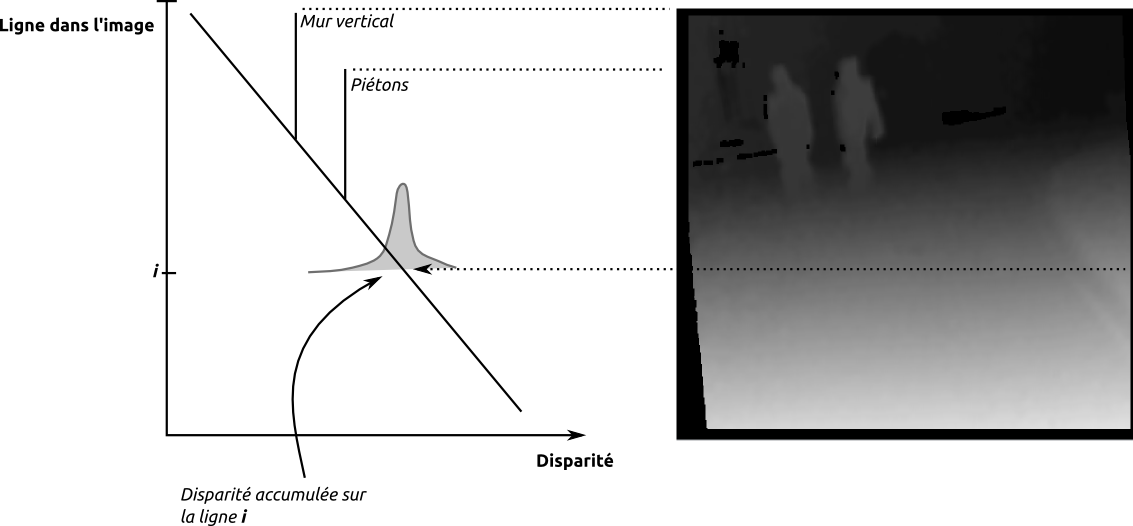
\includegraphics[width=0.9\textwidth]{Chapter2/graphics/v-disparity.png}
	\caption{Représentation schématique de la \og V-disparité\fg{}}
	\label{fig:ch2_v_disp}
\end{figure}

\subsubsection{Détection de l'espace navigable}
La détection des obstacles peut être réalisée au travers de son dual, la détection de l'espace navigable. Cette tâche s'apparente dans le domaine de la perception visuelle à une segmentation de l'image, connaissant \textit{a priori} l'aspect original de la zone à segmenter. On peut en effet supposer que le véhicule est initialement sur un espace navigable, et que cette propriété se propage par récurrence. De nombreuses approches sont possibles pour mener à bien cette tâche de segmentation, ce domaine de recherche étant l'objet de nombreux travaux. On pourra par exemple citer la croissance de région (Song et Civco, couplé à des méthodes d'apprentissage \cite{Song2004}) ou la technique dite de \emph{Graph Cut} (Grote \textit{et al.}, \cite{Grote2007}). Cette dernière consiste à considérer la zone à segmenter comme un graphe, à définir une fonction de coût liée à une subdivision de ce graphe, par exemple sur des critères de conservation de l'illumination, et à déterminer enfin la subdivision de ce graphe minimisant cette fonction de coût. On pourra enfin citer les approches basées sur la morphologie mathématique, notamment sur la technique dite de \emph{watershed} (inondation et ligne de partage des eaux), qui considère une image en niveaux de gris comme une carte de relief dont la segmentation est effectuée le long des lignes de partage des eaux. Cette approche est notamment proposée par Beucher et Yu (\cite{Beucher1994}).

\subsubsection{Détection de l'espace libre}
Une approche légèrement différente des propositions précédentes consiste à détecter l'espace libre, ou encore la position des premiers points occupés du champ de vision. Il est tout d'abord possible de se baser simplement sur une carte de disparité, telle que présentée sur la figure \ref{fig:ch2_disparity_map}, qui est analogue à une carte de profondeur relativement au plan image du capteur. Il est par ailleurs possible d'obtenir une telle carte avec une unique caméra. Dumortier \textit{et al.} (\cite{Dumortier}) proposent ainsi d'exploiter le calcul d'un flux optique dense. Ceci suppose de déterminer le mouvement du porteur entre les images utilisées pour le calcul du flux optique, ce qui est réalisé en deux étapes : le sol est tout d'abord détecté, dans une hypothèse de monde plan, ce qui permet ensuite de déterminer le mouvement en se limitant aux homographies. La connaissance de ce mouvement permet enfin le calcul de la carte de profondeur. \\
La détection de l'espace libre à partir d'une telle carte n'est ensuite pas immédiate, dans l'hypothèse où l'angle solide couvert par le système de vision est utilisé. Badino \textit{et al.} (\cite{Badino2007, Badino2009}) proposent pour cela de se situer dans l'espace réel, représenté par une grille d'occupation sur laquelle est projeté le résultat du calcul de disparité. La segmentation de l'espace libre est réalisée sur la grille d'occupation. 

\subsection{Détection par reconnaissance d'une signature visuelle} \label{sec:ch2_detection_reconnaissance}
La reconnaissance de forme est sans doute l'une des activités les plus naturelles de l'être humain, et pourtant difficilement transposable dans le monde algorithmique. Les usages rendus possibles par une telle capacité ont depuis longtemps motivé la recherche dans ce domaine, qui a grandement progressé et devient selon les domaines utilisable dans le domaine public (détection de visages, de panneaux, sont présents depuis plusieurs années dans l'électronique de grande consommation et l'automobile). \\
Les problèmes à résoudre sont multiples : les objets n'ont pas tous les mêmes singularités visuelles (on pourra penser par exemple à des spécificités de contour, de couleur, de texture, d'occultation partielle), et peuvent par ailleurs être l'objet de différenciations au sein d'une même classe, selon l'angle de prise de vue, les conditions de luminosité, ou du fait d'une variabilité intrinsèque (les visages, bien que partageant nombre de points communs, sont tous intrinsèquement différents). Il est donc capital dans ce domaine de pouvoir définir une signature à la fois discriminante et tolérante aux variations internes, nous en expliquons quelques principes par la suite.

\subsubsection{Correspondance avec un modèle}
Une approche possible est déterministe, dans le sens où il s'agit dans ce cas de choisir de manière arbitraire les critères supposés les plus pertinents, tant du point de vue de la forme de référence que de la norme utilisée. On peut par exemple, dans le cas de la reconnaissance d'une forme rectangulaire, choisir de se placer dans l'espace des gradients (plusieurs opérateurs étant communément utilisés à cet effet, tels les opérateurs de Sobel, Scharr ou Canny), définir notre référence comme la réponse de la forme recherchée à l'opérateur choisi, et définir notre vraisemblance par la somme des différences au carré (le problème de l'échelle pouvant par exemple être mitigé par une approche par pyramide d'images, ou par un algorithme en deux étapes, déterminant initialement l'échelle de l'objet à reconnaître). De nombreuses évolutions sont possibles, tant du point de vue de l'espace de mesure que de la mesure de vraisemblance, et la littérature présente de nombreuses méthodes devenues classiques (détection de lignes de marquage dans l'espace de Hough, détection de route par uniformité, ..). On pourra par exemple citer l'utilisation de gradients et d'un modèle déterministe pour détecter des feux tricolores (de Charette et Nashashibi, \cite{Charette2009}) ou les lignes de marquage (Vacek \textit{et al.} \cite{Vacek2006})\\

La mise en œuvre de cette méthode est cependant difficile dans le cas de formes à reconnaître non normalisées, pour des objets déformables par exemple, ou si certains aspects de l'apparence de l'objet ne sont simplement pas maîtrisés par l'opérateur. Par ailleurs, les choix initiaux des critères de reconnaissance (gradient, aplats, lignes droites, etc), s'ils sont souvent choisis par intuition, ne sont pas nécessairement optimaux. Une seconde approche historique, maintenant largement dominante dans le cas de la détection des piétons notamment, consiste à passer par une étape d'apprentissage automatisée chargée de déterminer les critères optimaux parmi un ensemble de caractéristiques arbitraires.

\subsubsection{Apprentissage}
Trois éléments restent arbitraires dans la plupart des méthodes proposées dans la littérature, qui limitent leur exhaustivité : \\
\begin{itemize}
	\item {\textit{Descripteur utilisé:}\\} 
	de nombreuses caractéristiques sont extractibles d'une image, par exemple un gradient (souvent utilisé sous la forme d'histogramme selon l'orientation, appelé HOG -Histogram of Oriented Gradients- dans la littérature, voir par exemple \cite{Dalal2005}), un motif local binaire (LBP - Local Binary Pattern, \cite{Wang2009}), un histogramme du flux optique (\cite{Dalal2006b}) ou encore des couleurs sur un voisinage (\cite{Walk2010}). L'utilisation de l'ensemble des caractéristiques exploitables n'est en général pas possible, du fait des grandes dimensions d'un tel système. Certains opérateurs sont alors choisis de manière arbitraire comme une base d'apprentissage, leurs mérites respectifs n'étant discernables qu'après expérimentation.\\

	\item {\textit{Optimisation de la signature discriminante:}\\}
	plusieurs méthodes sont possibles pour déterminer les critères de détection optimaux à partir de l'expression des descripteurs sur un grand nombre d'images. Deux approches sont principalement présentes dans l'état de l'art. La première est dite \og en cascade\fg{}, par combinaison successive de classifieurs dits \og faibles \fg{} (AdaBoost, introduit par Freund et Shapire \cite{Freund1997}). La seconde cherche à déterminer, dans l'espace vectoriel créé par les vecteurs de caractéristiques, la frontière (linéaire ou non) dissociant le mieux les positifs des négatifs (SVM - Support Vector Machine, voir par exemple une revue de Wojek \cite{Wojek2009}).\\

	\item {\textit{\og Sur-apprentissage\fg{}:}\\}
	la base de donnée sur laquelle l'optimisation est réalisée n'est bien sûr pas parfaite, tant du point de vue des situations présentes que des fréquences d'apparition. Des bases très importantes (plusieurs dizaines de milliers d'images) sont utilisés pour limiter les conséquences de cette spécialisation, mais un entraînement trop spécifique est toujours possible.\\
\end{itemize}

La reconnaissance d'objets par apprentissage a fait l'objet de nombreux travaux ces dernières décennies, et permet aujourd'hui d'obtenir des résultats probants. Il s'agit cependant d'une méthode nécessitant une connaissance \textit{a priori} de l'aspect de l'objet recherché, ce qui en limite par définition la généralité. On pourra cependant signaler une approche récente consistant à exploiter les techniques d'apprentissage en temps réel pour assurer un suivi d'objet dans le temps, suite à une première détection (voir notamment \cite{Hamdoun2010, Kalal, Kalal2009}).

\subsubsection{Exemple : HOG-SVM}
L'une des approches les plus utilisées dans la détection de piétons est basée sur une subdivision de l'image en cellules élémentaires, dans lesquels on représente les orientations du gradient de l'image par un histogramme. L'ensemble des cellules subdivisant l'image constitue alors, une fois les histogrammes concaténés, un vecteur de dimension très importante (>600 par exemple). Une illustration est présente sur la Figure \ref{fig:ch2_HOG_SVM} \footnote{Illustrations issues de travaux du CAOR-Mines Paristech - A. Breheret}, dans laquelle on représente tout d'abord le gradient de l'image (l'orientation du gradient étant représentée par une couleur), puis les différentes valeurs de l'histogramme des orientations au sein de chacune des cellules élémentaires (en niveaux de gris). Dans le cas d'un SVM linéaire, il s'agit de trouver les coordonnées de l'hyperplan distinguant de manière optimale les positifs des négatifs. La détection de la forme apprise est ensuite déterminée par la réponse du descripteur concaténant l'ensemble des histogrammes de gradients relativement au vecteur appris par le SVM.

\begin{table}
	\begin{center}
			\begin{tabular}  {c}
				\begin{subfigure}{0.75\textwidth}
					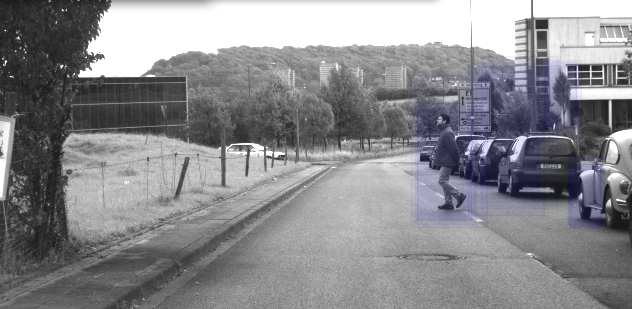
\includegraphics[width=\textwidth]{Chapter2/graphics/pedestrian_hog_pict.png} 
					\caption{Exemple de scène dans laquelle les piétons doivent être détectés. Les réponses à un détecteur initial (classification AdaBoost \cite{Freund1997}) sont représentées en bleu.}
				\end{subfigure}	
				\\ \\
				\begin{tabular} [t]{lcr}
					\begin{subfigure}{0.2\textwidth}
						\captionsetup{justification=raggedright}
						
\includegraphics[width=0.9\textwidth]{Chapter2/graphics/pedestrian_hog_grad.png} 
						\caption{Gradients orientés. La couleur représente l'orientation.}
						\vspace{10pt}
					\end{subfigure}	
					&
					\begin{subfigure}{0.2\textwidth}
						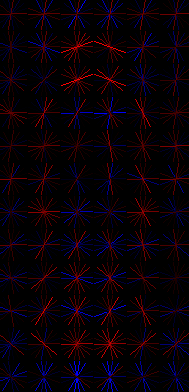
\includegraphics[width=0.9\textwidth]{Chapter2/graphics/hog_svm.png} 
						\captionsetup{justification=raggedright}
						\caption{Vecteur appris par SVM. Valeurs positives en rouge, négatives en bleu}
					\end{subfigure}	
					&
					\begin{subfigure}{0.2\textwidth}
						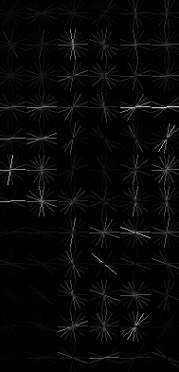
\includegraphics[width=0.9\textwidth]{Chapter2/graphics/pedestrian_hog_hog.png} 
						\captionsetup{justification=raggedright}
						\caption{Amplitude de la réponse de chacune des cellules au descripteur HOG-SVM}
					\end{subfigure}
				\end{tabular}
			\end{tabular}
	\end{center}
	\caption{Exemple d'utilisation d'un détecteur HOG+SVM}	
	\label{fig:ch2_HOG_SVM}
\end{table}

Cette méthode a de très nombreuses applications dans le domaine de la détection des piétons, et est d'ores et déjà exploitée dans des produits commercialisés. L'augmentation de ses performances est néanmoins toujours l'objet de recherches, la prise en compte de la grande variabilité d'apparence des piétons et de déformabilité de leur signature visuelle représentant des sources d'améliorations possibles.

\subsection{Détection du mouvement}
Une autre méthode consiste à se concentrer sur la détection d'un mouvement dans la scène. Ce mouvement peut être intrinsèque, c'est à dire indépendant du mouvement du porteur (ce qui implique de déterminer celui-ci), ou bien intriqué mais singulier (dans ce cas on ne détermine pas le mouvement propre, mais on peut le dissocier du mouvement perçu porté par les objets statiques). Il est par ailleurs possible d'utiliser une ou plusieurs caméras. \\

La détection d'objets mobiles à partir d'un point de vue statique est une première étape, notamment résolue dans la littérature en faisant appel à une soustraction des parties approximativement constantes de l'image. Les premières propositions dans ce domaine sont relativement anciennes, et introduisent notamment des techniques de morphologie mathématique pour traiter les problèmes de bruit et de segmentation (voir Allen par exemple \cite{Allen1994}). La contrainte d'immobilité du point de vue est cependant très forte, et rend cette approche inutilisable dans de nombreuses applications de robotique par exemple. \\

D'autres techniques proposent de prendre en compte d'un flux optique dense, et notamment des corrélations locales de celui-ci, relativement indépendantes du mouvement du porteur au niveau d'un objet. Pauwels (\cite{Pauwels2004}) propose ainsi une segmentation des objets ayant un mouvement propre, à partir du flux optique d'une unique caméra. Un estimateur robuste (exploitant la fonction de coût de Tukey, aussi appelée \og biweight\fg{} ou bicarré) est utilisé. \\

L'usage de plusieurs caméras simplifie l'estimation de l'ego-motion en présence de points marginaux, et peut par ailleurs permettre d'estimer relativement simplement la position approximative des objets mobiles postérieurement à leur détection. Badino (\cite{Badino2008}) propose une estimation dans l'espace du vecteur vitesse des objets observés, une fois l'ego-motion estimée et la position des points dans l'espace obtenue par triangulation. Bak (\cite{Bak2011}) propose de se fonder sur les variations de position dans l'espace image d'un dispositif de stéréo-vision, c'est à dire à la fois sur le flux optique (après compensation de l'ego-motion) et sur la variation de disparité au niveau d'un élément donné. De même, Agrawal (\cite{Agrawal2007}) propose, une fois estimé le mouvement propre de manière robuste, de détecter les objets mobiles dans l'espace de la disparité. Il se base pour cela sur la différence entre l'apparence attendue, du fait de l'observation précédente et du mouvement estimé, les parties de l'image différant de la prédiction effectuée pour un environnement rigide étant donc supposés mobiles. De manière relativement similaire, mais non dense, Lenz \textit{et al.} (\cite{Lenz2011}) proposent de se baser sur les positions successives de points d'intérêt dans l'espace, une fois pris en compte le déplacement du véhicule, pour détecter les objets mobiles.

\subsection{Localisation}
La localisation au sein d'un environnement connu est un problème récurrent de la robotique, que de nombreuses équipes ont résolu de manière différente. On décrit ici quelques unes des méthodes présentes au sein du domaine de la vision, mais ce problème est également adressable par quantité d'autres capteurs, notamment par l'utilisation d'un télémètre laser. Dans le cas de la vision donc, on pourra dissocier une approche par points d'intérêts et une approche par optimisation comme étant les plus présentes dans l'état de l'art. \\

Une approche par points d'intérêt consiste à extraire de l'environnement à cartographier des éléments singuliers des différentes localisations possibles, ces éléments étant identifiés par des descripteurs visuels (par exemple SIFT ou SURF, présentés dans la section \ref{sec:ch3_Détection_points_intérêt}). Il s'agit ensuite d'établir un ordonnancement de ces descripteurs à même d'autoriser une localisation rapide suite à une observation. Ceci passe souvent par la réalisation d'un graphe, dont l'ordonnancement reflète la proximité des environnements, de manière à converger très rapidement lors de la recherche sur le graphe vers un ensemble de descripteurs corrects lors de l'observation de quelques-uns d'entre eux. L'approche la plus souvent retenue pour décrire une localisation donnée est celle du \og sac de mots\fg{}, par analogie à un texte qui serait décrit par l'ensemble des mots le constituant, sans notion d'ordonnancement. De même, une scène est alors décrite par l'ensemble des descripteurs présents, sans ordonner ceux-ci les uns par rapport aux autres. La localisation de l'observation peut alors être réalisée en prenant en compte l'ensemble des descripteurs présents par rapport à ceux présents dans le \og sac de mot\fg{} enregistré, par un système de vote (\cite{Filliat2007}). Cette approche peut être réalisée en temps différé, ou en temps réel, par exemple pour pouvoir détecter une fermeture de boucle dans un dispositif de SLAM visuel (\cite{Mei}, \cite{Mei2010}). L'utilisation de descripteurs spécifiques à une scène donnée peut également être réalisée en considérant un continuum de descripteurs (par opposition à une segmentation de ceux-ci en \og sac de mots\fg{}), des critères géométriques de proximité permettant dans ce cas une représentation ordonnée des descripteurs présents importante pour la robustesse de la localisation (\cite{Sinha2012}). \\

Il est donc également possible d'exploiter une approche par optimisation, pour assurer une tâche de localisation  dans un environnement connu. On se place alors dans l'espace du capteur considéré (dans le plan image donc), l'erreur de position étant alors obtenue  par les défauts de correspondance entre l'observation et l'image enregistrée (\cite{Cherubini2010}). Cette méthode peut être généralisée par l'utilisation de sphères d'images, couvrant tout l'angle solide (\cite{Meilland2011}) autour du porteur. Une approche similaire, mais n'utilisant pas l'intégralité de l'image, est également possible (\cite{Dayoub}). Dans cette approche, une pyramide (variation d'échelle de la plus grossière à la plus précise) peut être utilisée pour accélérer la localisation, en plus d'une hiérarchisation des acquisitions de référence sous la forme de graphe. Une fonction de salience est par ailleurs utilisée pour ne conserver que les éléments discriminants de l'image et accélérer le calcul. Cette approche est notamment présente dans la littérature sous le nom de \textit{Visual Servoing} (asservissement visuel).

\subsection{Suivi dans le temps des objets mobiles} \label{sec:ch2_suivi_objets_mobiles}
% Différents aspects à prendre en compte :
% - filtrage dans le temps des observations (pour se prémunir des fausses détections par exemple). Nécessaire car les observations ne sont pas parfaites
% - suivi dans le temps des associations entre les objets présents et les observations
% --------
% Explication des enjeux
Différents aspects sont à prendre en compte pour répondre à cette problématique. Les détections d'objets mobiles ne sont en effet pas parfaites, et un cadre algorithmique permettant d'estimer la réalité des observations et leur cohérence dans le temps est indispensable. Le nombre d'objets présents est initialement inconnu, et peut varier dans le temps, l'algorithme utilisé pour les estimer devant donc être capable de prendre en compte des probabilités d'apparition et de disparition non nulles. Il est par ailleurs nécessaire d'estimer l'association dans le temps entre les observations consécutives, celle-ci n'étant pas toujours un produit direct de l'observation, ou bien soumis à un bruit de mesure. La plupart des approches proposées dans la littérature prennent en compte la nature stochastique des observations dans un cadre probabiliste, mais de nombreuses méthodes sont possibles et cette notion probabiliste n'est pas strictement obligatoire. Une revue très complète de différentes méthodes présentes dans la littérature est notamment visible dans un manuscrit de Bailey (\cite{Bailey2002}), on en présente quelques unes parmi les plus connues dans les paragraphes suivants.\\

% Exemples d'associations 'binaires'
% association \og locale\fg{}
\subsubsection{Associations uniques et locales}
Il est tout d'abord possible de ne considérer qu'une fonction d'association \og binaire\fg{}, dans le sens où l'hypothèse la plus vraisemblable est la seule prise en compte. De nombreuses méthodes sont possibles pour déterminer ces associations unitaires.\\
Celle-ci peut être déterminée par une méthode relativement directe, en exploitant notamment des seuillages spatiaux et temporels pour réduire les fausses détections, comme mis en œuvre par Lenz \textit{et al.} dans une publication récente (\cite{Lenz2011}). Les associations entre les observations et l'état précédent du système sont effectuées selon la technique dite GNN (\emph{Global Nearest Neighbour}, Voisin le plus proche globalement), c'est à dire que chacune des observations est associée à l'objet dont la position prédite est la plus proche. Chaque association est dans ce cas exclusive, une observation étant associée à un unique objet pré-existant et réciproquement. Cette méthode peut être prise en défaut en présence de nombreuses cibles proches, et les associations peuvent notamment être erronées lors d'occultations.\\
% association globale\fg{}
\subsubsection{Associations uniques globales}
Bailey \textit{et al.} (\cite{Bailey2006}) proposent de prendre en compte individuellement la contribution d'éléments distinctifs de la cible précédente et de la nouvelle observation, par exemple des caractéristiques géométriques ou des descripteurs visuels. L'association d'une cible à une observation peut alors être vue comme un ensemble de correspondances entre chacun de leurs descripteurs. L'ensemble des correspondances possibles dessine un graphe, la méthode de Bailey \textit{et al.} stipulant que l'association retenue sera celle faisant le plus consensus (dans le sens du nombre de descripteurs associés), sous la contrainte du respect de contraintes géométriques éventuelles.\\
D'autres méthodes sont possibles pour ne retenir que l'ensemble des associations unitaires étant globalement optimales, se basant souvent sur la définition d'une fonction de vraisemblance qui sera maximisée pour déterminer les associations les plus probables. Cette fonction de vraisemblance peut notamment inclure un facteur de proximité, mais aussi d'identification par classe, ou par dimensions par exemple. Le calcul de l'optimum global n'est pas trivial, du fait du très grand nombre de degrés de liberté du problème en présence de cibles multiples.\\

% Associations Combinées Probables (Probabilistic Data Association)
\subsubsection{Associations combinées probables}
Le bruit de mesure et la proximité des cibles rendent parfois difficile la détermination d'une unique correspondance entre les états précédents et courants. La modélisation de cette méconnaissance peut se faire de manière probabiliste, plusieurs associations étant envisagées tandis qu'une combinaison de celles-ci est finalement retenue. Cette méthode est connue sous le nom de PDA (\emph{Probabilistic Data Association}, Association probabiliste des données), et fut initialement proposée par Bar-Shalom (\cite{Bar-Shalom1975, Bar-shalom}). La théorie développée par cette méthode est proche du filtre GM-PHD proposé ultérieurement (\emph{Gaussian Mixture - Probability Hypothesis Density}, Filtre par densité de probabilité des hypothèses, modélisées par des mixture de gaussiennes), présenté dans la section \ref{sec:ch5_GMPHD}. Cette méthode a été initialement proposée par Vo et Ma (\cite{Vo2006a}) comme une propagation approximative du filtre PHD. Les hypothèses de présence d'objet mobile ou d'association sont dans ce cas représentées par des ensembles finis aléatoires (RFS, \emph{Random Finite Set}) de Gaussiennes, les hypothèses finalement les plus probables étant conservées. On pourra notamment citer Ivekovic et Clark (\cite{Ivekovic2009}) pour une application de ces principes dans l'espace de la disparité, et Chen \textit{et al.} (\cite{Chen2011}) pour une application dans le domaine du suivi d'objets détectés visuellement. Bien qu'envisageant de manière probabiliste plusieurs hypothèses d'associations, cette méthode modélise néanmoins l'état final de chacune des cibles par une unique Gaussienne, c'est à dire que les hypothèses multiples ne sont pas propagées dans le temps.\\

% Exemples d'algorithmes \og Multi-hypothesis tracking \fg{}
\subsubsection{Suivi d'hypothèses multiples}
La gestion d'associations probablement multiples a été initialement proposée par Reid \cite{Reid1979}, et est maintenant connue sous le nom de MHT (\emph{Multi-Hypothesis Tracking}, suivi d'hypothèses multiples). Dans cette approche, les hypothèses d'associations sont corrigées \textit{a posteriori}, compte tenu des observations ultérieures. Cet algorithme propose donc une étape de génération d'hypothèses, dans le cas où une association unique n'est pas satisfaisante, puis une étape de confrontation des hypothèses existantes aux observations. Une étape de simplification des hypothèses existantes est également présente, approximation qui permet de simplifier le traitement en temps réel des associations possibles. Ces principes sont également visibles dans le filtre GMPHD que nous présentons dans la section \ref{sec:ch5_GMPHD}, bien que celui-ci ne propage pas d'hypothèses multiples.\\

% Algo bayésien sur une grille
% Pas centré sur chacune des cibles, mais plutôt sur chaque élément de l'espace
\subsubsection{Algorithmes probabilistes, denses en 2 dimensions}
Le problème de l'association des mesures dans le temps, de la gestion des fausses détections et d'un nombre fluctuant de cibles présentes peut être envisagé de manière très différente. Il est ainsi possible de se concentrer sur un échantillonnage spatial de variables telles que l'occupation, plutôt que sur l'évolution de chacune des cibles présentes. La finalité est similaire (l'estimation de la probabilité d'occupation en tout point de l'espace permet de détecter les obstacles potentiels, par exemple), mais le procédé est bien différent. Plusieurs approches basées sur ce principe sont présentes dans la littérature, par extension au travail fondateur de Moravec et Elfes (\cite{Moravec1985, Moravec1988}) sur les grilles d'occupation. Chen \textit{et al.} (\cite{Chen2006}) proposent d'exploiter un filtre bayésien en deux dimensions connu sous le nom de BOF (\emph{Bayesian Occupancy Filter}, Filtre d'occupation Bayésien), qui définit à partir d'une discrétisation de l'espace dans le plan navigable l'état propagé le plus probable. Il faut pour cela définir des probabilités de transitions entre différentes positions spatiales, compte tenu des variables estimées, qui comprennent dans ce cas l'occupation et la vitesse. Toutes les cellules représentant l'espace navigable discret sont alors propagées. En suivant un principe relativement similaire, mais en se limitant à la propagation de cibles déjà observées sur un maillage discret, Gate \textit{et al.} (\cite{Gate2009}) proposent eux aussi un algorithme Bayésien d'estimation de l'état d'un environnement dynamique. Cette approche est présentée de manière plus approfondie dans ce manuscrit, dans la section \ref{sec:ch5_Bayésien_2D}. Une méthode similaire basée sur la théorie des croyances est par exemple proposée par Moras et al. (\cite{Moras2011a}).

\section{Perception globale : systèmes SLAMMOT} \label{sec:ch2_Algo_total}
La littérature emploie couramment le terme SLAMMOT (\emph{Simultaneous Localisation And Mapping and Mobile Objet Tracking}, Localisation, construction d'une carte et suivi des objets mobiles simultanément) pour désigner les algorithmes permettant de résoudre dans une approche cohérente (avec un certain degré d'intrication) les problématiques de positionnement de points spécifiques de la scène et d'estimation du mouvement, tout en détectant et en suivant les objets mobiles. Nous reprendrons cet acronyme anglophone dans les paragraphes suivants. Ces algorithmes ont pour particularité commune de fonctionner dans un repère cartésien orthonormal, du fait de la reconstruction de l'environnement qui y prend place. On peut à cet égard les opposer à certaines des méthodes présentées précédemment dans lesquelles les estimations sont réalisées dans un repère lié au capteur utilisé. Cette reconstruction dans un espace tiers peut alourdir le calcul, et rendre plus difficile l'estimation des erreurs, mais est notamment importante pour fusionner des informations provenant de capteurs très différents.\\

% Présenter la suite
On présente dans les sections suivantes des méthodes proposées pour résoudre le problème SLAMMOT avec une ou plusieurs caméras. Cette distinction n'est pas anodine, car ce problème peut être résolu avec une unique caméra, mais des restrictions s'appliquent alors. Tous les paramètres du problème ne sont en effet pas directement accessibles avec une unique caméra, du fait de la nature projective du procédé d'imagerie, et certains mouvements ou dispositions géométriques peuvent être problématiques. On pourra par exemple se référer au travail de Lin et Wang (\cite{Lina}), qui comparent un dispositif SLAMMOT mono-vision et stéréo-vision par rapport à une référence à base de télémètre laser. On pourra également se référer à la complète étude d'observabilité de Vidal \textit{et al.} (\cite{Vidal2002}), qui couvre la faisabilité de la détection d'un ou plusieurs objets indépendant à partir de deux vues. On pourra enfin se référer à l'étude d'observabilité de Solà Ortega et Devy (\cite{Ortega2007}). L'observation d'un objet mobile dont le vecteur vitesse est identique à celui du référentiel de la caméra est un exemple simple de situation non définie pour un système SLAMMOT mono-caméra.

\subsection{Monovision} \label{sec:ch2_SLAMMOT_mono}
Les tâches imputables à un système SLAMMOT sont difficiles à résoudre avec une unique caméra, du fait des nombreuses inconnues introduites dans le système par l'opération de projection sur le système d'imagerie. Il est cependant possible de résoudre ce problème théoriquement, avec certaines limitations, notamment sur le ratio entre les observations de points mobiles et statiques, et sur les mouvements du porteur. Ce système n'est, par exemple, pas résoluble dans le cas d'une observation à partir d'un porteur statique, dans lequel les objets mobiles peuvent être détectés mais non positionnés sans d'autres hypothèses. D'autres situations sont par ailleurs problématiques, par exemple lors de l'observation d'un objet ayant le même vecteur vitesse que le porteur de la caméra. \\

Les SLAM visuels basés sur un filtre de Kalman étendu (\ref{sec:ch4_filtrage}), sur le modèle de l'article fondateur de Davison \cite{Davison2003}, proposent une façon élégante de résoudre ce système. Cet algorithme a notamment été complété par Montiel (\cite{Montiel}), et contient assez naturellement la possibilité de détecter et de suivre les objets mobiles. Tous les points à positionner, ainsi que la position courante de la caméra, sont présents dans cette approche dans le vecteur d'état d'un filtre. L'étape de mise à jour du filtre doit être robuste, afin de restreindre les observations prises en compte aux objets statiques, mais elle fournit la possibilité de mettre à jour indépendamment la mesure correspondant à des points marginaux (par exemple déterminés par une approche par consensus de type RANSAC), et par là même d'en estimer la position au fil du temps. Il s'agit notamment de l'approche proposée par Wangsiripitak et Murray (\cite{Wangsiripitak2009}). On pourra notamment trouver une évaluation d'une telle approche par Lin et Wang (\cite{Lina}), notamment par comparaison avec un dispositif multi-caméras. On constate dans cette référence qu'une approche par caméras multiple est toujours plus performante dans la détection et le suivi d'objets mobiles qu'une approche mono-caméra.

\subsection{Stéréovision et caméras multiples}\label{sec:ch2_SLAMMOT_stereo}
L'utilisation de caméras multiples résout en général le problème d'observabilité soulevé dans le paragraphe précédent, dans lequel les observations d'une unique caméra peuvent être prises en défaut. Différentes stratégies sont cependant possibles pour détecter, positionner et suivre les objets mobiles. \\

Il est tout d'abord possible de détecter les objets mobiles \emph{a posteriori}, c'est à dire consécutivement à une observation dans laquelle tous les éléments observés sont initialement indistincts. La mise en relation de chacune de ces observations avec l'état du système (dans le cadre par exemple d'un filtre bayésien) permet alors de dissocier les points probables des points marginaux. C'est une approche présente dans de très nombreuses publications basées sur un SLAMMOT par EKF, notamment là encore par Lina (\cite{Lina}), ou bien par  Solà Ortegua et Devy (\cite{Ortega2007}) ou encore Marquez et al. \cite{Marquez2012}. Cette approche de la détection et du suivi des objets mobiles est également possible lorsque l'étape dite de \og SLAM\fg{} est confiée à un processus d'optimisation, comme le montrent notamment Zou et al. (\cite{Zou}) dans un dispositif exploitant de multiples caméras sans lien rigide. \\

Il est à l'inverse possible de se baser sur une détection \emph{a priori} des objets mobiles pour résoudre le problème du SLAMMOT, en exploitant par exemple les avancées récentes des systèmes d'apprentissage et de reconnaissance. Il s'agit dans ce cas de reconnaître des objets probablement mobiles, et de supposer qu'il s'agit là de l'ensemble des objets que l'on souhaite suivre dans notre tâche SLAMMOT. C'est notamment l'approche suivie par Schindler (\cite{Schindler2010}), qui utilise une détection préalable des piétons (dont la silhouette est apprise par SVM sur un descripteur de type HOG, comme décrit dans \ref{sec:ch2_detection_reconnaissance}) pour les extraire d'un système de SLAM visuel. Le suivi probabiliste des piétons est confié à un réseau bayésien, l'ensemble améliorant significativement les performances d'une détection de piéton seule.

\section{Approche proposée} \label{sec:ch2_Approche_globale}
\subsection{Observations sur les méthodes existantes}
De nombreuses approches ont été présentées ici, bien que trop rapidement, répondant à tout ou partie des problématiques initiales : comment acquérir des informations sur l'environnement courant, puis détecter, positionner et suivre les objets mobiles ? Certaines de ces tâches sont individuellement très bien maîtrisées avec les algorithmes présents dans la littérature, comme la reconstruction de l'environnement statique autour du porteur, ou la gestion d'éléments mobiles parmi les points suivis. Il existe cependant très peu d'approches globales, incluant la prise en compte des objets mobiles, centrée sur la perception des obstacles et à même de fournir suffisamment d'informations pour répondre à une tâche de planification de trajectoire. Une extension des propositions existantes pour répondre à cette problématique n'est en général pas triviale, la plupart des limitations soulevées (prise en compte des objets mobiles, faible densité des observations, positionnement dans l'espace des obstacles détectés,..) étant intrinsèques à la méthode proposée. \\

On tentera par la suite de répondre à cette problématique, en proposant une démarche globale centrée sur ces besoins :\\

\begin{itemize}
	\item {\emph{Suivi fiable dans le temps:\\}}
	Du fait de nos besoins en matière de perception de la dynamique, le suivi dans le temps d'éléments de la scène observée est primordial. Il s'agit de l'unique source d'informations externes du système pour répondre aux besoins de localisation, cartographie et suivi des objets mobiles. Contrairement aux besoins de certaines approches, qui ne déterminent, par exemple, pas le mouvement à partir du flux optique ou de la disparité, la qualité du suivi de point est très importante dans une approche globale.\\
	
	\item{\emph{Grande densité d'échantillonnage:\\}}
	Ce point sera précisé dans le chapitre suivant, mais on remarque ici que la tâche de détection des obstacles suppose bien sûr que nous suivions et positionnons suffisamment d'éléments de la scène pour que les obstacles soient présents dans l'échantillonnage réalisé. Certaines approches de SLAMMOT proposées précédemment sont à notre en sens trop limitées en termes de nombre de points traités pour servir de base à une détection des obstacles, et nous tenterons de répondre à ce besoin par une approche différente.\\
	
	\item {\emph{Gestion des objets mobiles:\\}}
	Il existe de nombreuses approches de type SLAM répondant à la problématique précédente, du fait de leur gestion d'un nombre très important de points (à la suite notamment de la publication fondatrice de Mouragnon et Lhuillier \cite{Mouragnon2006} et de l'algorithme PTAM de Klein et Murray \cite{Klein2007}). Ces méthodes ne considèrent cependant pas, en général, l'évolution dans le temps de la position des points. De même, certaines méthodes se basent sur une combinaison de SLAM épars combiné à un calcul dense de carte de profondeur, grâce à un dispositif de stéréo-vision (voir Lategahn et al. \cite{Lategahn2011} par exemple). L'absence du suivi de l'intégralité des points dans le temps n'autorise pas la prise en compte de leur mouvement. Notre démarche nécessite donc un suivi dans le temps de l'intégralité des points positionnés.\\
	
	\item{\emph{Traitement temps réel, ou pouvant raisonnablement l'être:\\}}
	La navigation autonome d'un véhicule génère de nombreux besoins qui doivent être traités en temps réel, parmi lesquels la perception de l'environnement. Celle-ci forme en effet, avec la planification de trajectoire et les moyens de déplacement un asservissement cyclique, conditionné par le plus lent de ses éléments. Nous souhaitons finalement proposer un algorithme capable de résoudre les problématiques précédentes tout en conservant un temps de calcul de l'ordre de la période d'acquisition, afin de pouvoir assurer une exécution en temps réel. Cette contrainte ne doit pas nécessairement être respectée stricto sensu, s'agissant d'un travail de recherche. On s'attachera cependant à proposer une approche pouvant raisonnablement prétendre à cette durée d'exécution.\\
\end{itemize}

\subsection{Étapes principales de l'approche retenue}
% Annoncer la méthode :
% - on se base sur des points suivis dans le temps et sur les paires d'image
% - on sépare l'ego-motion et la localisation des points
% - on utilise les méthodes les plus modernes de filtrage multi-cibles
L'approche proposée tient compte des nombreux travaux introduits dans les paragraphes précédents, tout en se focalisant sur l'acquisition d'une connaissance de l'environnement proche à même d'assurer une navigation autonome. Il ne s'agit donc pas d'une méthode centrée sur la cartographie absolue, ou sur l'estimation d'une trajectoire.\\

\begin{enumerate}
	\item{\textbf{Informations visuelles:}\\}
	On se base tout d'abord sur une détection et un suivi, dans le temps et sur une paire de caméras, de points d'intérêt. Si les méthodes à base d'apprentissage obtiennent d'ores et déjà de très bons résultats en matière de détection d'obstacles, il ne s'agit pas d'une approche générale, dans le sens où elle se limite aux classes d'objets déjà identifiées. Notre travail s'est concentré sur une méthode plus agnostique, de détection des objets mobiles, quelconques. Une fusion de ces techniques est cependant possible, et sans doute souhaitable. \\
	Nous avons, par ailleurs, fait le choix d'un suivi de points spécifiques, et non de l'intégralité de l'image, pour cette première étape d'acquisition d'informations sur l'environnement. Un flux optique dense fonctionne, en effet, grâce à une contrainte d'optimisation globale, qui assure un suivi optimal en moyenne mais ne garantit pas la qualité des suivis individuels. Dans le cas du suivi dans le temps de points visuellement non définis (par une absence de contraste local notamment), un suivi dense fournira par exemple un résultat dont la qualité n'est pas vérifiable, ce que nous souhaitons éviter. On devine par ailleurs sur la figure \ref{fig:ch3_OF_Farneback} que tous les éléments du flux optique ne sont pas nécessairement corrects dans cette approche dense. Il est ensuite difficile de déterminer les éléments fautifs, et nous avons donc choisi de nous concentrer sur une approche parcellaire. Un suivi dense dans le temps est par ailleurs délicat à mettre en œuvre en temps réel, et cette exécution rapide constituait un de nos prérequis initiaux.\\
	Le maintien d'un ensemble de points d'intérêt décrivant la scène proche du porteur constitue ainsi une première étape de notre algorithme, qui sera détaillée dans le chapitre \ref{sec:ch3}.\\
	
	\item{\textbf{Estimation du mouvement et de l'environnement statique:}\\}
	L'influence des mouvements du porteur dans l'évolution de la scène perçue, et l'intérêt de l'accumulation des informations dans le temps, motivent ensuite le chapitre \ref{sec:ch4}. L'état de l'art des méthodes de détermination du mouvement d'une caméra est important et sera présenté, ainsi que l'approche que nous proposons. Celle-ci vise à répondre à des besoins de rapidité et de robustesse, tout en exploitant le cadre précédent de suivi de points d'intérêt sur une paire stéréoscopique, mais nous ne développons pas d'estimation globale de la trajectoire. \\
	La multiplicité des observations (les mêmes points d'intérêt peuvent être observés de manière répétée) nous amène ensuite à proposer un filtrage de la position des points observés, dans la mesure où ceux-ci sont statiques. On peut en effet dissocier à cet étape de détermination du mouvement les points respectant un mouvement d'ensemble cohérent, et à l'inverse isoler de potentiels points mobiles.\\
	
	\item{\textbf{Gestion des éléments mobiles:}\\}
	Les points ne respectant pas une transformation rigide de la scène peuvent être confondus avec des erreurs de suivi, et ne sont pas vraiment exploitables en l'état car trop nombreux et non structurés. On propose donc dans le chapitre \ref{sec:ch5} un cadre algorithmique pour détecter tout d'abord les points mobiles, puis les segmenter en objets relativement rigides (car affichant un vecteur vitesse approximativement uniforme, la tolérance présente lors des étapes de segmentation permettant de prendre en compte les légères disparités présentes sur des objets déformables, tels que des piétons); et enfin filtrer et suivre dans le temps ces éléments mobiles. La segmentation proposée exploite les informations qui découlent des étapes précédentes, et qui ne sont pas communes dans la littérature. On dispose en effet de nuages de points échantillonnés dans le temps, et dont les associations temporelles sont connues, ce qui nous permet de proposer une détection des points mobiles et une segmentation spécifiques.\\	
\end{enumerate}


On dispose finalement d'une représentation en trois dimensions des éléments fixes de la scène, sous la forme de dizaines de milliers de points positionnés dans l'espace, correspondant aux dernières secondes de perception visuelle. La position et le déplacement du véhicule porteur dans cet environnement sont estimés. On dispose également d'informations sur des objets mobiles présents dans le voisinage du porteur, sous la forme de boîtes englobantes en trois dimensions, dont la trajectoire est estimée ainsi que le vecteur vitesse courant. Une représentation schématique de l'algorithme et du plan suivi est visible sur la figure \ref{fig:ch2_approche_proposée}.

\begin{figure} 
	\centering
	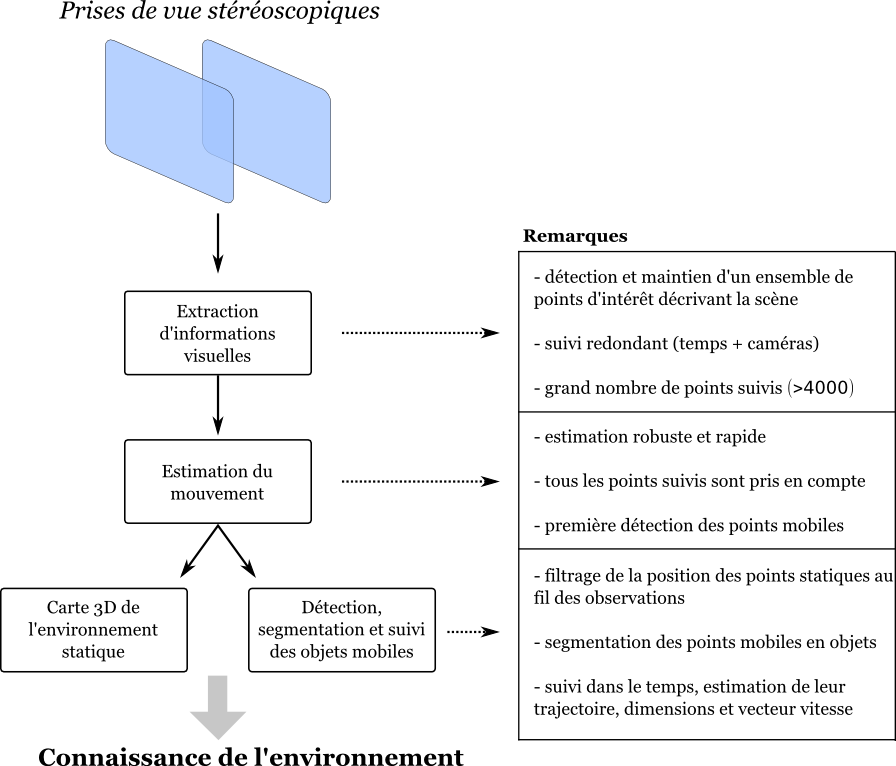
\includegraphics[width=0.98\textwidth]{Chapter2/graphics/overall_scheme_2.png}
	\caption{Vue générale de l'approche proposée}
	\label{fig:ch2_approche_proposée}
\end{figure}

\chapter{Acquisition des indices visuels} 
\label{sec:ch3}
\vspace{10pt}

\minitoc
\clearpage

% % % % % % % % % % % % % % % % % % % %
%	Acquisition des indices visuels	  %
% % % % % % % % % % % % % % % % % % % %
\section{Introduction}
On s'intéresse ici à quelques unes des approches présentes dans la littérature dans le domaine de l'acquisition d'informations visuelles, avant de préciser l'algorithme que nous proposons et avons mis en œuvre. De nombreuses informations peuvent être acquises visuellement (reconnaissance d'objets, détection de mouvement, etc), et il s'agit d'un domaine de recherche particulièrement important ces dernières années. Comme présenté dans la section \ref{sec:ch2_Approche_globale}, nous nous sommes concentrés sur un moyen d'acquisition d'informations quasi-ponctuelles à partir d'images successives, et ne nous ne détaillerons donc pas l'ensemble des différentes techniques accessibles. On pourra cependant retenir que d'autres approches, parfois complémentaires à la nôtre, sont possibles, et qu'il s'agit d'une perspective de développement de notre travail à ne pas négliger.\\

Les indices visuels qui constituent le premier élément de notre chaîne algorithmique peuvent être définis de diverses façons, notamment selon les algorithmes utilisés. Il s'agit dans tous les cas d'éléments singuliers de l'image, c'est-à-dire différentiables de leurs voisins (selon une métrique qui considère souvent une forme de corrélation sur leur voisinage). Cette singularité est le plus souvent seulement locale, c'est-à-dire qu'il n'y a pas nécessairement unicité de ce point, même accompagné de son voisinage proche, dans l'image entière. On notera par la suite ces indices visuels \og points d'intérêt \fg{}. Il s'agira paradoxalement d'éléments ayant tous les attributs de la ponctualité dans l'espace, mais étant définis sur un ensemble d'éléments du plan image. \\
On présentera tout d'abord un état de l'art des algorithmes présents dans la littérature, après avoir introduit la notion de densité d'informations perçues, et expliqué notre choix de nous concentrer sur la détection et le suivi d'éléments singuliers de l'image. Une seconde partie sera consacrée à la présentation de l'algorithme que nous proposons pour assurer le suivi fiable de nombreux points d'intérêt. Une dernière partie sera enfin consacrée à une évaluation des performances obtenues, et à l'explication de quelques spécificités techniques mises en œuvre.

\section{État de l'art}
On présente dans ce qui suit les techniques présentes dans la littérature pour assurer la détection et le suivi de points singuliers à partir de séquences d'images. On montre tout d'abord que l'utilisation de la vision est pertinente pour l'acquisition d'informations ponctuelles dans l'espace, quand bien même ces informations ne représentent pas l'intégralité des données acquises. On présente ensuite différents algorithmes, épars et denses, qui permettent de détecter et suivre dans le temps ces éléments de l'image.

%\subsection{Vision comme source d'informations ponctuelles} \label{sec:ch3_Densité d'informations perçues}
%On revient ici sur la pertinence du choix de la vision comme capteur de perception, principalement sur le critère de la densité d'information perçue. Bien d'autres critères sont possibles pour juger les capteurs perceptifs (portée, rapport signal/bruit, domaine d'utilisation, type d'information perçue..), mais nous détaillons à dessein un point qui pourrait sembler défavorable pour une solution visuelle par rapport à certains capteurs répandus dans la littérature.

\subsection{Densité d'informations} \label{sec:ch3_densité_informations}
On introduit tout d'abord une mesure de densité d'échantillonnage de l'information, en nombre d'échantillon par degré d'angle solide. Cette mesure nous permettra de quantifier différentes approches dans le domaine de la vision (notamment dites \emph{dense} ou \emph{éparses}), mais aussi de les comparer avec des approches différentes, par exemple par télémètre laser de type \emph{Velodyne}. Cette comparaison est à replacer dans le cadre plus général d'un dispositif algorithmique de perception de l'environnement, ceci étant accessible par différents moyens.

\subsubsection{Densité de mesure:}
On définit naturellement la densité $\delta$ par : $\delta = \frac{\mathcal{N}}{\Omega}$, avec $\mathcal{N}$ le nombre moyen de points échantillonnés et $\Omega$ l'angle solide couvert. L'angle solide est calculé comme le ratio, pour une sphère de rayon 1, entre la surface de la sphère couverte par l'ouverture angulaire du dispositif en question et la surface totale de la sphère, soit $4\Pi$. Une illustration de ce calcul est visibles sur la figure \ref{fig:ch3_densité}.

\begin{figure}
	\begin{center}
		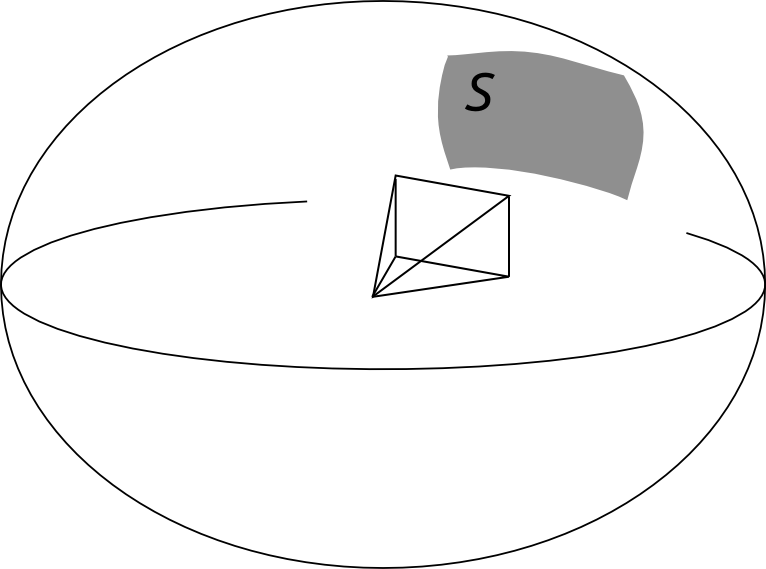
\includegraphics[width=0.6\textwidth]{Chapter3/graphics/calcul_density.png}
		\caption{Illustration du calcul de densité d'acquisition. La surface S correspond à la zone échantillonnée par le dispositif représenté, au sein de la sphère unité. Le calcul de l'angle solide est le ratio de ces deux surfaces}
		\label{fig:ch3_densité}
	\end{center}
\end{figure}

L'angle solide d'un dispositif de perception au sein de la sphère unité est potentiellement complexe, si la surface correspondante est quelconque. Il s'écrit formellement :
\begin{equation}
	\Omega = \int\limits_{S} \int \frac{ \vec{r} \cdot \vec{n} dS} {r^3}
\end{equation}
(avec $\vec{r}$ le vecteur entre le centre de la sphère et l'élément infinitésimal de surface intégré, et $\vec{n}$ le vecteur unité normal à la surface en ce point). Le calcul est simplifié pour les dispositifs que nous allons considérer par la suite, du fait de l'angle solide couvert, lorsqu'il s'agit d'un intervalle défini sur deux axes. En notant $\Delta_{\Phi}$ l'ouverture angulaire verticale, et $\Delta_{\Theta}$ l'ouverture angulaire horizontale, l'angle solide couvert s'écrit alors :

\begin{equation}
	\Omega = 4 \cdot \arcsin( \sin(\frac{\Delta_{\Phi}}{2}) \sin(\frac{\Delta_{\Theta}}{2}))
\end{equation}

Dans le cas d'un capteur ayant une couverture à $360^\circ$, l'angle solide $\Omega$ s'écrit :
\begin{equation}
	\Omega = 4 \Pi \cdot \sin(\frac{\Delta_{\Phi}}{2})
\end{equation}

\subsubsection{Comparaison selon les capteurs:}
Considérons maintenant quelques capteurs et usages typiques des tâches de perception (la densité est exprimée en nombre de points par millistéradians):

\begin{table}[H]
	\centerline {
		\begin{tabular}{|c | c| c | c | c | c |} 
			\hline
			\pbox{1cm}{Capteur\\ } & \pbox{8cm}{Nombre \\ de points} & \pbox{8cm}{Ouverture \\ verticale} & \pbox{8cm}{Ouverture \\ horizontale} & \pbox{8cm}{Angle \\ solide} & Densité (pt/msr) \\
			\hline
			Caméra - Épars 		& 100 	& 55$^\circ$		& 40$^\circ$ 	& 0.1 	& 1\\
			\hline
			Caméra - Épars 		& 4k 		& 55$^\circ$ 		& 40$^\circ$ 	& 0.1 	& 40\\
			\hline
			Caméra - Dense 		& 300k 	& 55$^\circ$ 		& 40$^\circ$	& 0.1 	& 3000\\	
			\hline
			Velodyne - HDL32 	& 128k 	& 26.8$^\circ$ 	& 360$^\circ$ & 0.5 	& 225\\	
			\hline
			Velodyne - HDL64 	& 256k 	& 26.8$^\circ$	& 360$^\circ$ & 0.5 	& 550\\ 
			\hline
			Kinect 						& 300k 	& 57$^\circ$ 		& 43$^\circ$ 	& 0.1 	& 2700\\ 
			\hline
			Radar 						& 125 	& 25$^\circ$ 		& 10$^\circ$ 	& 0.01 	& 10\\ 
			\hline
		\end{tabular}
	}
	\caption{Quelques exemples de densités d'échantillonnage}
	\label{tab:ch3_comp_densité}
\end{table}

On a choisi dans le tableau \ref{tab:ch3_comp_densité} une caméra de résolution 640x480 dans le cas d'un traitement dense, cette valeur pouvant être révisée à la hausse dans nombre de publications récentes, au prix de besoins accrus en termes de puissance de calcul (\cite{Lategahn2011}). Les valeurs de \emph{100} et \emph{4000} points choisis dans les algorithmes dits épars se veulent typiques de diverses implémentations de SLAM visuel, typiquement selon les approches par filtrage ou optimisation (cf. section \ref{sec:ch4_state_of_art}). Les ouvertures angulaires choisies dans le cas de la vision correspondent à un angle de vue \og standard\fg{} (d'une optique de focale 35mm dans le standard 24mm*36mm), et sont à moduler selon les installations expérimentales. Ces valeurs permettent de bien poser la problématique et les besoins en termes de suivi de points, dans le cadre de la vision. L'usage des lasers de type "Velodyne" est en effet courant dans les recherches sur l'automatisation des véhicules, et sa densité d'informations a prouvé être suffisante dans de nombreux usages urbains (Spinello et Siegwart \cite{Spinello2010}, Azim et Aycard \cite{Azim}, Mertz \textit{et al.} \cite{Mertz2013}). Elle nous servira donc de référence pour évaluer la pertinence d'une approche ponctuelle de la perception visuelle. Les caractéristiques des capteurs radar notamment utilisés dans l'automobile ont été repris de \cite{Schneider2006}.

\subsubsection{Quelques remarques:}
On pourra, par exemple, distinguer les points suivants :
\begin{itemize}
	\item On compare dans le tableau \ref{tab:ch3_comp_densité} des densités d'échantillonnage entre un capteur télémétrique à balayage et un système de vision, sans tenir compte des limites de ces derniers, qui peuvent diminuer l'échantillonnage effectif. En pratique de nombreux facteurs peuvent impacter la qualité de la perception visuelle, notamment : \\
	
		\begin{itemize} \renewcommand{\labelitemii}{$\cdot$}
			\item{\emph{les conditions d'illumination:\\}}
			La dynamique d'un capteur d'imagerie étant communément limitée à environ 12 bits, les parties de l'image dont l'éclairement relatif à l'éclairement moyen est au delà de cette dynamique maximale seront perçues comme uniformes, aucun point ne pouvant alors être suivi. Un exemple en est présenté sur la figure \ref{fig:ch3_saturated_pic}, sur laquelle un histogramme de la luminosité des pixels permet de mettre en évidence une saturation de l'acquisition dans les tons clairs.\\
			
			\item{\emph{la dynamique du porteur ou des éléments mobiles:\\}}
			Dans le cas d'un mouvement trop rapide, la vitesse d'obturation peut ne pas être suffisante pour rendre négligeable le mouvement perçu pendant le temps d'intégration. L'objet imagé est dans ce cas mal défini, jusqu'à éventuellement compromettre la possibilité même d'un suivi de points caractéristiques dans le temps. Cette mauvaise définition peut également avoir un impact sur la détection de points d'intérêt, comme présenté dans \cite{Mei2010}.\\
			
			\item{\emph{la "détectabilité" propre des objets:\\}}
			Le traitement des informations visuelles est sensible (quelque soit la solution technique retenue) à l'aspect des objets, et peut notamment être mis en défaut par des objets parfaitement uniformes.\\
		\end{itemize}

	\item L'utilisation simultanée d'un nombre raisonnable de caméras (6 caméras par exemple, si tant est que la puissance de calcul nécessaire soit disponible, et que les critères précédents soient remplis) permet de couvrir un angle solide équivalent aux capteurs de type \og Velodyne\fg{}. C'est une approche retenue par Meilland \textit{et al.} (\cite{Meilland2011}) par exemple.\\
	
	\item On ne parle ici que d'une mesure possible pour évaluer la quantité d'un type d'informations perçues, pas nécessairement de l'ensemble des informations que l'état de l'art parvient à en extraire. De très nombreuses applications sont ainsi disponibles pour exploiter des images, ou des nuages de points. Il s'agit donc d'une base de comparaison arbitraire, en aucun cas exhaustive.
\end{itemize}

\begin{figure}
	\begin{center}
		\begin{subfigure}{0.48\textwidth}
			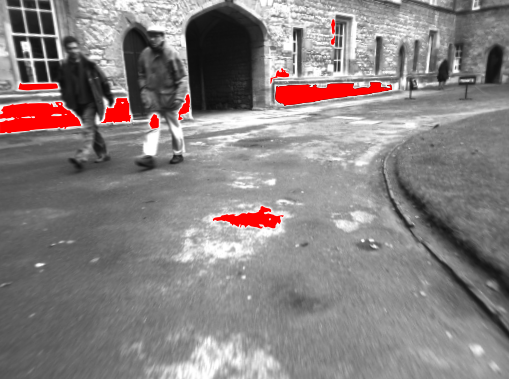
\includegraphics[width=\textwidth]{Chapter3/graphics/NewCollege_overexposed.png} 
		\end{subfigure}
		~
		\begin{subfigure}{0.48\textwidth}
			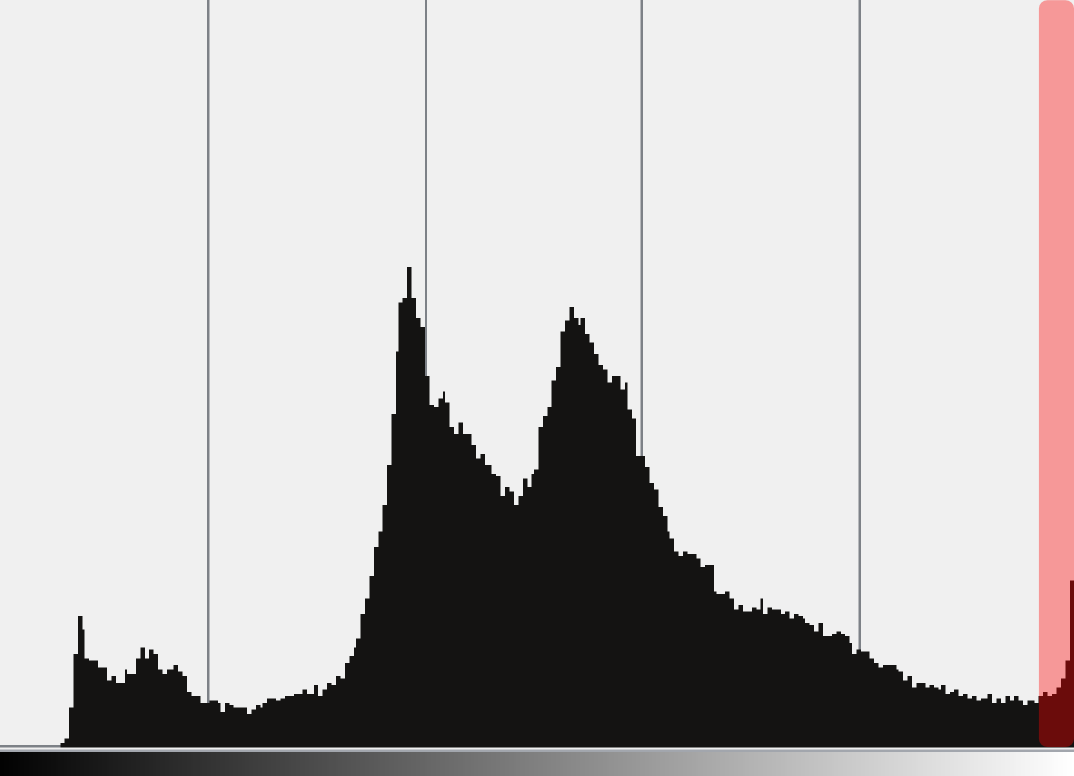
\includegraphics[width=\textwidth]{Chapter3/graphics/NewCollege_histogram_red.png} 
		\end{subfigure}
		
		\caption{Illustration de la saturation possible du capteur d'imagerie. Un histogramme de la répartition des valeurs de niveaux de gris des pixels est représenté, la saturation étant visible de part une accumulation des valeurs extrêmes de l'histogramme. Les zones saturées sont représentées en rouge sur l'image, et correspondent à l'accumulation sur la droite de l'histogramme des valeurs de luminosité}	
		\label{fig:ch3_saturated_pic}
	\end{center}
\end{figure}

\subsection{Algorithmes \og épars\fg{}} \label{sec:ch3_Vision_epars}
Cette partie est consacrée aux algorithmes basés sur un suivi de points singuliers, par opposition aux suivis denses (\ref{sec:ch3_Flux_optique_dense}) qui sont par ailleurs de plus en plus populaires dans la littérature. On pourrait tout d'abord se demander pourquoi une telle approche est-elle seulement nécessaire, puisque le suivi de l'ensemble des points est possible ? Différents arguments sont possibles, on citera notamment les critères de qualité du suivi de points, primordiale dans notre approche, ainsi que les contraintes de temps de calcul. 

\subsubsection{Sélection des points d'intérêt:} \label{sec:ch3_Détection_points_intérêt}
Dans le cas où tous les points d'un image ne sont pas considérés, il semble important d'en assurer une sélection pertinente en préalable à toute opération. Tous les points d'une image n'ont en effet pas la même valeur selon les usages, mais plusieurs critères sont possibles. En règle générale, les points indistinguables de leur voisins ont une contribution très faible à l'information portée par l'image (par exemple dans le cas d'une zone contiguë dans laquelle la réponse du capteur est saturée), et l'on peut raisonnablement supposer qu'ils n'auront jamais d'intérêt à être mis en avant. En revanche, la sélection des points "<principaux\fg{} parmi ceux restant n'est pas simple, et pourrait être envisagée selon deux aspects : qualité intrinsèque des points au sein de l'image, et leur adéquation à l'usage visé. Schmid et al. (\cite{Schmid2000}) proposent ainsi deux critères pour la sélection de points : la quantité d'information présente (liée au degré d'entropie locale) et la répétabilité, considérant donc par ce deuxième critère que l'usage qu'il est fait des points détectés (par exemple SLAM, ou suivi d'objet) rentre aussi en compte. Il s'agit de l'approche que nous avons suivi dans notre comparaison de trois détecteurs (\ref{sec:ch3_Eval_PI}), prenant en compte le temps de calcul nécessaire à la détection d'un nombre de points donnés, et la qualité de ceux-ci dans une perspective de suivi dans le temps.\\

La détection de points d'intérêts présente dans la littérature s'articule autour de trois grandes approches, que l'on peut résumer brièvement par les quantités suivantes: 
\begin{itemize}
	\item{\emph{Contour:\\}} 
	les points d'intérêt se situent sur des points remarquables des contours détectés dans l'image. \\

	\item{\emph{Intensité:\\}}
	les valeurs d'intensité sur un voisinage sont discriminantes, par exemple la réponse à une fonction d'auto-corrélation.\\

	\item{\emph{Optimisation paramétrique:\\}}
	on pré-suppose une forme arbitraire pour les points recherchés, cette forme définit une fonction de coût dont les extrema sont recherchés dans l'image.\\
\end{itemize} 

On présente dans la suite quelques uns des détecteurs de points d'intérêt les plus utilisés, mais cet état de l'art ne peut être exhaustif dans le cadre de ce manuscrit de thèse, et le lecteur pourra se reporter sur la littérature du domaine pour plus d'informations (par exemple \cite{Tuytelaars2007} et \cite{Schmid2000} pour une revue, \cite{Shi2002} \cite{Bay} \cite{Lowe1999a} et \cite{Rosten} pour des articles de référence, ou encore \cite{Sood2008} pour une application au SLAM visuel). 

\paragraph{Harris:\\}
Le détecteur de Harris s'intéresse aux points singuliers en terme de gradient, et considère pour cela une fonction de coût, basée sur l'intensité des pixels sur un voisinage donné. Celle-ci exploite une proposition de Moravec (\cite{Moravec1980}), qui propose en 1980 de considérer la somme des différences au carré (\emph{Sum of Squared Differences}, souvent noté SSD) autour du point considéré. Harris (\cite{Harris1988}) introduit en 1988 une approximation de la dérivée seconde de cette fonction de coût, en utilisant la matrice Hessienne :
\begin{equation} \label{eq:ch3_Harris_H}
	H_{Harris} = \left[ 
		\begin{array}{cc}
		\widehat{I_x}^2 & \widehat{I_x} \widehat{I_y} \\
		\widehat{I_x} \widehat{I_y} & \widehat{I_y}^2  
		\end{array} 
	\right]
\end{equation}
avec $\widehat{I_x}$ un opérateur réalisant la différence des valeurs d'intensités sur un voisinage selon l'axe $x$. La réponse du détecteur est alors, avec $k$ un paramètre d'ajustement :
\begin{align}
	R &= Det(H) - k*Tr(H)^2
	k &= \textnormal{paramètre d'ajustement}
\end{align}

Cette réponse dépend de l'amplitude des valeurs propres de la matrice $H$, sans pour autant en nécessiter le calcul explicite. Ce détecteur peut se montrer trop sensible au bruit présent dans l'image, auquel cas un lissage peut être initialement appliqué. Il est également possible de choisir la fonction de différence $I$ pour mieux prendre en compte ce problème. Un défaut de ce détecteur, développé dans la suite de notre étude, est en outre sa sensibilité à des forts gradients unidimensionnels. Celle-ci peut l'amener à sélectionner des points dont l'unicité sur un voisinage proche n'est pas garantie.

\paragraph{Shi et Tomasi : "Good Features To Track"\\}
Ce détecteur a été présenté dans \cite{Shi2002}, et se base sur le détecteur précédent. Dans cet article, Shi et Tomasi ont réalisé une étude très complète de cas pratiques de suivi d'éléments d'une scène, en considérant notamment les altérations visibles entre le même élément physique imagé de plusieurs points de vue. Leur étude portant sur des transformation affine des images les amène à recommander l'usage des valeurs propres  $\lambda_1$ et $\lambda_2$ les plus faibles de l'équation \ref{eq:ch3_Harris_H} comme fonction de coût, soit :
\begin{equation}
	R = min(\lambda_1, \lambda_2)
\end{equation}

\paragraph{\emph{SIFT} (Scale Invariant Feature Transform):\\}
Cet algorithme a été proposé par Lowe et al. (\cite{Lowe1999a}), et comprend une étape de détection et une étape d'extraction de descripteur, c'est-à-dire une signature caractéristique et répétable d'un élément de l'image, qui peut permettre de le retrouver sur une autre prise de vue. Nous ne nous intéresserons qu'à la détection de points d'intérêt de part notre approche, et le descripteur SIFT (qui signifie Scale Invariant Feature Transform) ne sera pas utilisé.\\
La procédure retenue pour la détection de points SIFT passe par la réalisation d'une pyramide d'images, obtenues par une convolution de l'image originale avec un noyau gaussien suivie d'un sous-échantillonnage. Le nombre d'étages de la pyramide d'image est l'un des paramètres de l'algorithme. Chaque étage contient plusieurs versions de l'image à la même échelle, ayant subit un nombre plus ou moins important de convolutions par un noyau gaussien. Ceci permet ensuite d'utiliser la fonction \og Différence de Gaussiennes\fg{}, en soustrayant à une image de référence une image plus convoluée, les points d'intérêt SIFT étant alors recherchés parmi les extrema locaux de cette fonction. On pourra remarquer que les points obtenus sont alors théoriquement invariants d'échelle, la convolution par un noyau gaussien étant par ailleurs l'un des moyens les plus appropriés de mise à l'échelle d'une image (\cite{Lindeberg1994}). La recherche de points SIFT peut donc se résumer à la recherche de points saillants dans l'espace des différentes échelles de l'image. Cette recherche commence par l'échelle la plus basse, seuls les points saillants d'une échelle donnée sont ensuite recherché à l'étape supérieure. Une illustration de cet algorithme est visible sur la figure \ref{fig:ch3_SIFT}.

\begin{figure}
	\centerline{
		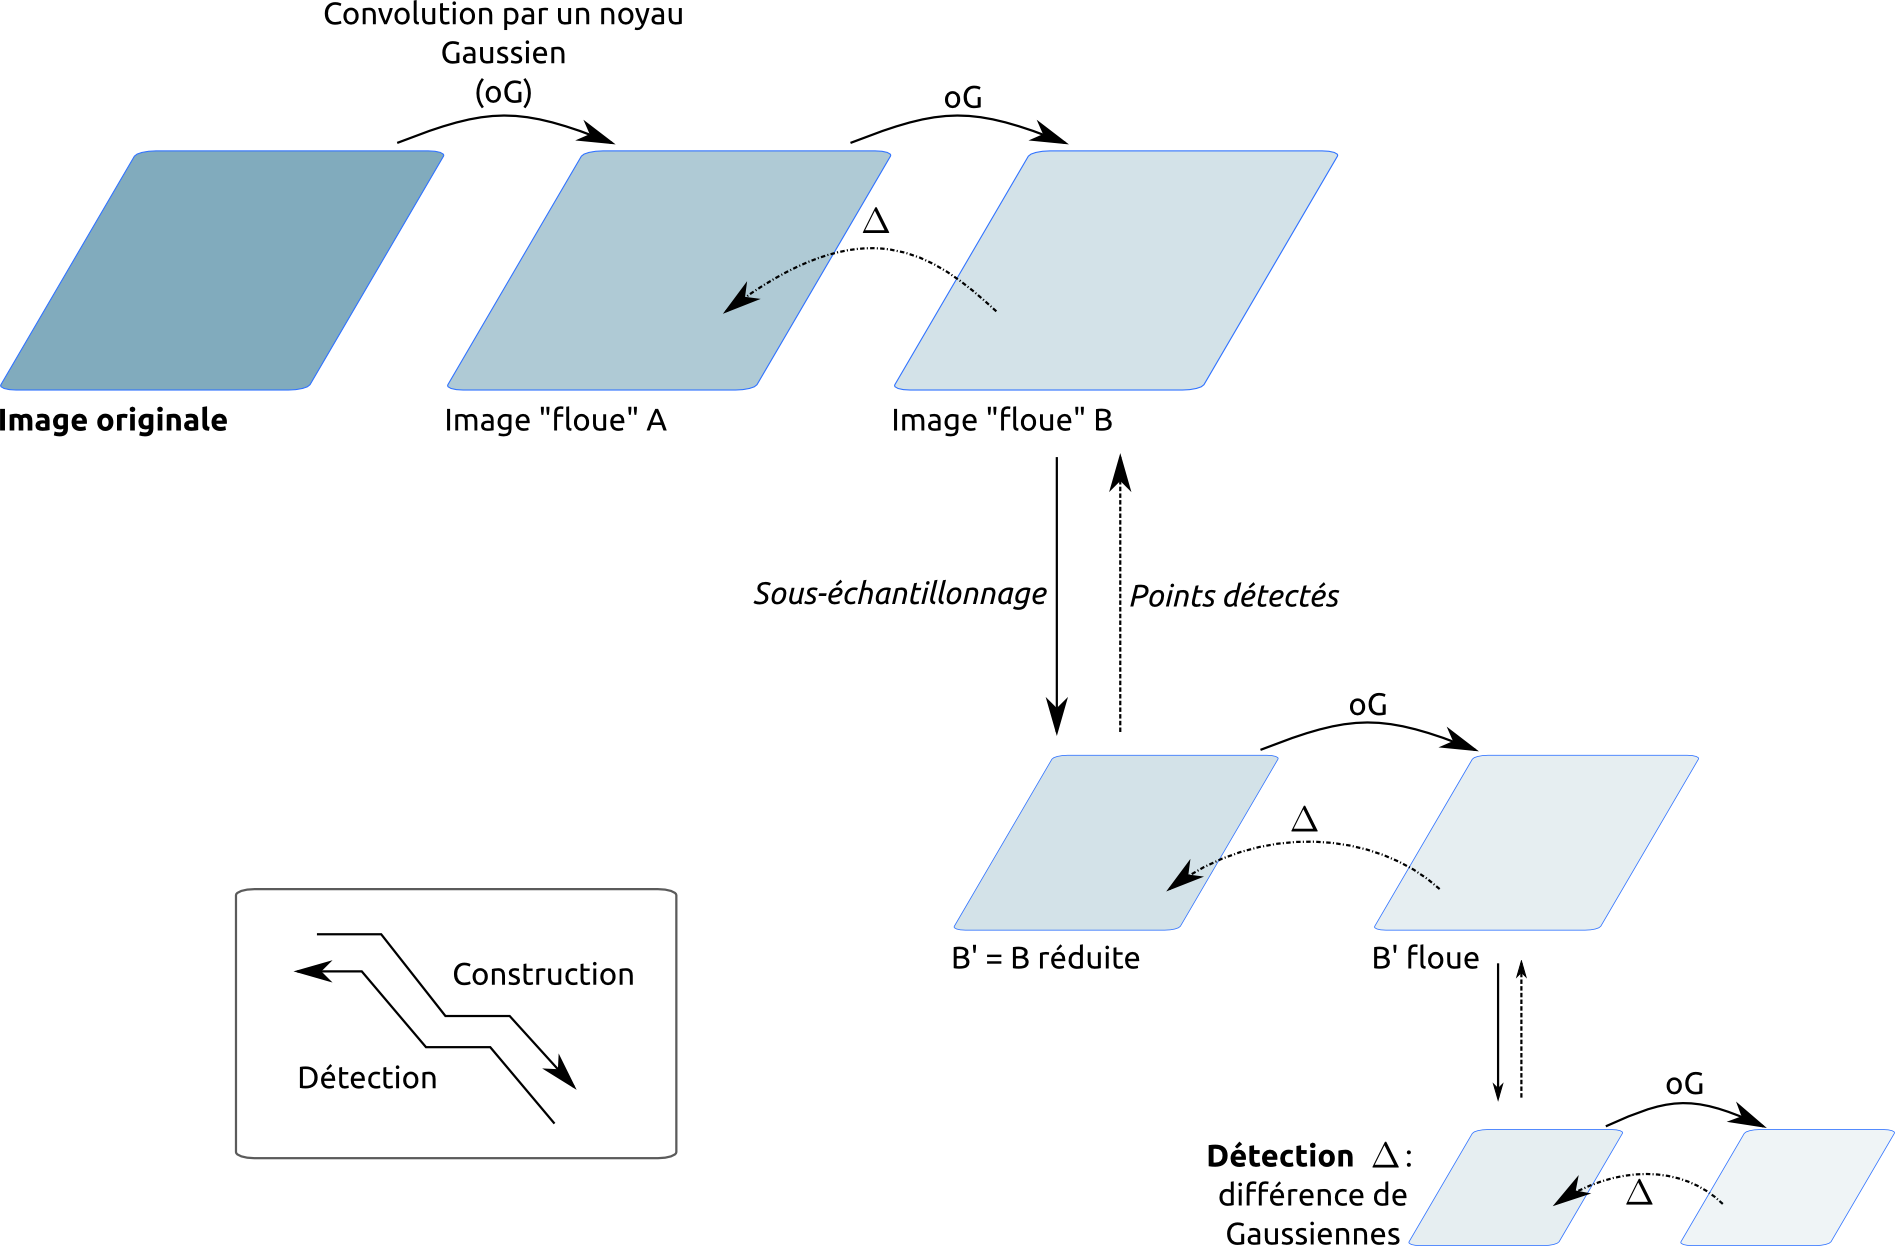
\includegraphics[width=0.9\textwidth]{Chapter3/graphics/SIFT.png}
		}
	\caption{Schéma de fonctionnement de l'algorithme SIFT}
	\label{fig:ch3_SIFT}
\end{figure}

\paragraph{\emph{SURF} (Speeded Up Robust Feature):\\}
Cet algorithme, présenté par Bay et al. dans \cite{Bay}, désigne lui aussi à la fois un détecteur de points d'intérêt et un descripteur. Nous ne nous intéresserons qu'à la détection de points d'intérêt dans cette partie, et ne ferons donc pas une description complète de SURF. \\
Bay propose de se baser sur la matrice hessienne de l'intensité, c'est-à-dire la matrice des dérivées partielles secondes de la fonction intensité. Il propose par ailleurs que cette matrice hessienne soit appliquée sur une image convoluée par une Gaussienne, et non l'image originale, la convolution par une gaussienne permettant une mise à l'échelle de l'image (et l'invariance du détecteur à celle-ci).

\begin{equation} \label{SURF_H}
	H_{SURF} = \left[ 
		\begin{array}{cc}
		L_{xx}(x, \sigma) & L_{xy}(x, \sigma) \\
		L_{xy}(x, \sigma) & L_{yy}(x, \sigma)  
		\end{array} 
	\right]
\end{equation}
avec $L_{xx}(x, \sigma)$ désignant la convolution de la dérivée seconde d'une gaussienne $\frac{\partial^2 g(x, \sigma)}{{\partial x}^2}$ avec l'image au point $P(x,y)$. \\

Bay  et al. proposent par ailleurs une approximation de cette matrice, suivant en cela un procédé similaire à la construction des points SIFT (\cite{Lowe1999a}), qui rend  $L_{xx}(x, \sigma)$ discrète et simplifie fortement son calcul. On note cette approximation $D_{xx}$ par la suite, comme proposé dans \cite{Bay}. Ce calcul est enfin réalisé par le biais d'une \emph{image intégrale} (procédé courant en traitement d'image consistant à enregistrer pour chaque pixel la valeur cumulée des pixels précédents) de l'application sur l'image complète de $D_{xx}$ ,  $D_{xy}$  et $D_{yy}$. Ce procédé permet de calculer les dérivées nécessaires sur l'intégralité de l'image, puis de calculer la valeur du détecteur en un point $P(x,y)$ par soustraction des valeurs voisines de l'image intégrale, ce qui minimise les calculs redondants lors d'une détection de points d'intérêt sur une image donnée.\\

La fonction de coût conduisant à la détection ou non d'un point d'intérêt est finalement une approximation du déterminant de H (équation \ref{SURF_H}), dont la justification est visible dans \cite{Bay} (le coefficient 0.9 visant à pondérer l'erreur faite dans le calcul de déterminant par la discrétisation):
\begin{equation} \label{eq:ch3_SURF_R}
	R = D_{xx} * D_{yy} - (0.9 * D_{xy})^2
\end{equation}
Un point d'intérêt est finalement sélectionné dès que la réponse $R$ du détecteur SURF (équation \ref{eq:ch3_SURF_R}) dépasse un seuil préalablement fixé.

\paragraph{\emph{FAST} (Features from Accelerated Segment Test):\\}
Le détecteur de points d'intérêt \emph{FAST} (Rosten et al. ,\cite{Rosten}) a été obtenu par apprentissage, et diffère en cela des définitions \og déterministes\fg{} des points Harris et SURF. Il se base cependant sur une observation \emph{a priori}, celle d'une recherche de points d'intérêts sous la forme de \og coins\fg{} contrastés. Cette recherche se fait en parcourant un cercle dit de Bresenham (discrétisé sur la matrice des pixels), comme initialement proposé dans \cite{Rosten2005}. Un coin se caractérise alors par un segment continu sur ce cercle de valeur relativement homogène, et nettement inférieure (ou supérieure) à celle du pixel central $P$, comme l'illustre la figure \ref{fig:ch3_FAST_illustration}.\\

Cette définition doit être testée sur l'ensemble des segments obtenus en parcourant le cercle de Bresenham pour valider l'existence ou non d'un \og coin\fg{} en son milieu. Chacun de ces tests constitue alors le nœud d'un arbre binaire, qui sera parcouru tant que le test précédent est positif. Cette structure permet donc un rejet rapide des  mauvais candidats, sans avoir nécessairement à effectuer l'ensemble des calculs nécessaires sur un voisinage, comme il est l'usage pour d'autres détecteurs. Cette caractéristique est intéressante en pratique, les points d'intérêt étant empiriquement très minoritaires dans une image. Rosten et al. proposent d'optimiser par apprentissage l'organisation de cet arbre de décision, afin que les réjections les plus probables soient effectuées plus avant, et évitent des calculs probablement inutiles. Cette optimisation a été réalisée dans le cas du détecteur \emph{FAST} par un réseau de neurones, et conduit à l'arbre binaire statique qui est maintenant couramment utilisé dans d'autres travaux (voir par exemple BRIEF, par Calonder et al. \cite{Calonder2010}, ou FREAK, par Alahi \cite{Alahi}).

\begin{figure}
	\centering{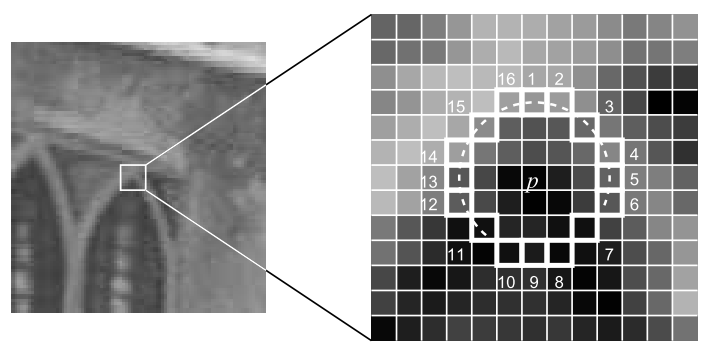
\includegraphics[width=0.68\textwidth]{Chapter3/graphics/FAST.png}}
	\caption{Une illustration partielle du détecteur FAST (source : Rosten\textit{ et al.} \cite{Rosten}). Les pixels surlignés de blanc représentent les extrémités des segments testés à partir du pixel central pour infirmer ou confirmer sa singularité.}
	\label{fig:ch3_FAST_illustration}
\end{figure}

\subsubsection{Suivi de points} \label{sec:ch3_suivi_de_points}
\paragraph{Par re-détection de points d'intérêt:\\}
Une première méthode consiste à utiliser la détection de points d'intérêt pour les images sur lesquelles le suivi doit être assuré, puis une mesure de similarité entre le point d'intérêt initial et les points d'intérêts détectés dans un voisinage donné sur la seconde image. Il s'agit par exemple de l'approche suivie par Davison dans le domaine du SLAM visuel (\cite{Davison2003}), ou plus récemment par Clipp, Nistér ou Mei par exemple (\cite{Clipp, Nister2006, Mei2010}). La détection peut dans ce cas se faire à l'aide des algorithmes présentés dans \ref{sec:ch3_Détection_points_intérêt}, tandis que la mesure de similarité peut prendre différentes formes, par exemple \textit{SSD} (\emph{Sum of Squared Differences}, somme des différences au carré) ou \textit{SAD} (\emph{Sum of Absolute Differences}, somme des différences absolues) ; normalisés par une soustraction de leurs valeurs moyennes en intensité pour rendre ce suivi plus robuste aux changements d'illumination.

%Mettant l'accent sur le suivi de points sur le plus grand nombre d'acquisitions possible, nous n'avons pas retenu cette approche, du fait du risque de disparition d'un point d'intérêt au fur et à mesure d'un changement de perspective, par exemple. Une autre méthode consiste à rechercher par optimisation la position d'un point sur une nouvelle image, sans supposer que celui-ci soit de nouveau détectable en tant que point d'intérêt prédominant.

\paragraph{Par optimisation itérative:\\}
Le suivi de points d'intérêt peut également prendre une autre forme, consistant à cherche l'optimum d'une fonction de vraisemblance autour de la position initiale du point d'intérêt. L'algorithme de référence dans cette approche a initialement été introduit par Lucas et Kanade (\cite{Lucas1981a}) sous la forme d'une descente de gradient, puis perfectionné par un algorithme pyramidal le rendant plus apte à suivre des mouvements importants par Bouguet (\cite{Bouguet2001a}). Cet algorithme suppose que l'illumination de l'image reste constante, mais cette condition peut éventuellement être relâchée par une adaptation de l'illumination moyenne (\cite{Zach2008}). \\

Cet algorithme est détaillé en annexe (\ref{sec:Annexe_klt}), mais nous pouvons d'ores et déjà remarquer qu'il s'agit d'une approche locale, pouvant relativement aisément être mise en défaut. On peut par exemple imaginer le cas du suivi d'un élément d'un motif répétitif, pour lequel de nombreux optimum locaux vont exister. Par ailleurs, cet algorithme suppose de descendre un gradient local pour ajuster la position recherchée, ce qui suppose donc qu'il soit bien défini. D'autres techniques d'optimisation sont possibles, prenant en compte une optimisation globale. On pourra citer une approche par Graph Cut (\cite{Freedman}, \cite{Boykov}, ou bien l'application \emph{a posteriori} de contraintes de régularité, qui nécessitent dans ce cas le calcul quasi-dense du flux optique (voir \ref{sec:ch3_Flux_optique_dense}).


\subsection{Algorithmes denses}\label{sec:ch3_Flux_optique_dense}
Le suivi de points peut également être réalisé de manière dense, c'est-à-dire que tous les points de l'image sont alors mis à contribution. Les méthodes présentées dans la section \ref{sec:ch3_suivi_de_points} sont évidemment généralisables, mais cette utilisation n'est le plus souvent pas souhaitable. Les suivis de points proposés consistent en effet en une optimisation locale, qui ne prend pas en compte la cohérence globale du suivi des points. Cette approche peut être mise en défaut lors du suivi de zones uniformes de l'image, pour lesquels les différents points de convergence de ces algorithmes locaux ne conserveront \textit{a priori} pas la contrainte de quasi-uniformité. Elle peut également être mise en défaut sur les zones bien définies et non-uniformes, mais pour lesquelles une répétition de motif propose plusieurs \og attracteurs\fg{} (suivi de points sur un damier par exemple). Les méthodes itératives (KLT) ou par re-détection peuvent dans ce cas converger vers un minimum local dépourvu de réalité physique. \\
Pour toutes ces raisons, de nombreuses contributions alternatives ont été proposées pour résoudre le problème du suivi dense de points dans une image, également appelé flux optique. Une étude approfondie serait hors de propos dans le cadre de ce manuscrit, mais on pourra en présenter quelques méthodes parmi les plus reconnues:

\paragraph{\emph{Horn-Schunk}:\\}
Cette technique fut initialement proposée dans \cite{Horn1981}, et se base sur une équation contraignant les changements de luminosité avec le mouvement perçu d'une partie de l'image. De fait, en supposant que la luminosité de chacun des éléments de la scène est inchangée, on constate aisément que le flux optique (le vecteur vélocité des déplacements perçus des éléments de l'image) doit alors être perpendiculaire au gradient de luminosité. Cette contrainte n'est cependant pas suffisante, car elle ne permet notamment pas la détermination du mouvement le long des lignes d'égale luminosité, et d'autres éléments sont donc nécessaires. \\
Supposant que le flux optique le long d'éléments homogènes de la scène devra être lui aussi homogène, Horn et Schunck (\cite{Horn1981}) proposent de prendre également en compte une contrainte de lissage, définie comme le carré du gradient de la vélocité : ${\frac{\partial{u}}{\partial{x}}}^2 + {\frac{\partial{u}}{\partial{y}}}^2$ et  ${\frac{\partial{v}}{\partial{x}}}^2 + {\frac{\partial{v}}{\partial{y}}}^2$ (avec $u$ et $v$ les deux composantes du déplacement sur l'image). La méthode de Horn et Schunk consiste alors à trouver le champ de vitesse $(u,v)$ minimisant les erreur cumulées de changement de la luminosité et du carré du gradient de la vélocité. En notant, comme dans l'article fondateur de Horn et Schunk, $E(x,y,t)$ la luminosité d'un point $P(x,y)$ de l'image au temps $t$, l'erreur $\Delta E$ que l'on cherche à minimiser sur chacun des pixels s'écrit, avec $\Lambda$ la contrainte de lissage que l'on fixe par ailleurs :\\

\begin{align}
	{\Delta E}_{Ill.}^2 &= 	\left( \frac{\partial E}{\partial x} \cdot u + \frac{\partial E}{\partial y} \cdot v + \frac{\partial E}{\partial t} \right)^2 \\
	{\Delta E}_{Cont.}^2 &= {\frac{\partial{u}}{\partial{x}}}^2 + {\frac{\partial{u}}{\partial{y}}}^2 \\
	{\Delta E}^2 &= 				{\Delta E}_{Ill.}^2 + \Lambda \cdot {\Delta E}_{Cont.}^2
\end{align}

Horn et Schunk montrent par ailleurs que le coefficient $\Lambda$ doit être de l'ordre de l'erreur attendue dans la détermination du vecteur de déplacement dans l'image.

\paragraph{\emph{Tenseur d'orientation}:\\}
Proposée initialement par G. Farneback (\cite{Farneback2000} puis \cite{Farneback}), cette méthode exploite une représentation en trois dimensions de l'évolution du vecteur vélocité $u$ dans le temps, sous la forme d'une matrice tensorielle, symétrique semi-définie et positive $T$. Cette matrice décrit l'évolution de la luminosité localement selon trois dimensions (espace et temps), de sorte que le vecteur vélocité peut en être déduit comme son vecteur propre associé à la valeur propre 0 (on suppose que la vélocité est conservée sur un même élément source). Farneback propose donc un mécanisme permettant de calculer l'ensemble des matrices $T$ de manière efficace, ainsi qu'une minimisation de ${u}^T T u$ conduisant à une estimation robuste du vecteur vitesse $\hat{u}$. Un exemple exploitant cette méthode est visible sur la figure \ref{fig:ch3_OF_Farneback}.\\

\begin{figure}
	\begin{subfigure}{0.48\textwidth}
		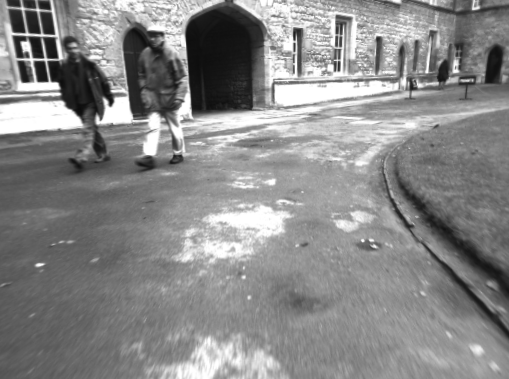
\includegraphics[width=\textwidth]{Chapter3/graphics/OF_Farneback_RAW.png} 
	\end{subfigure}
	~
	\begin{subfigure}{0.48\textwidth}
		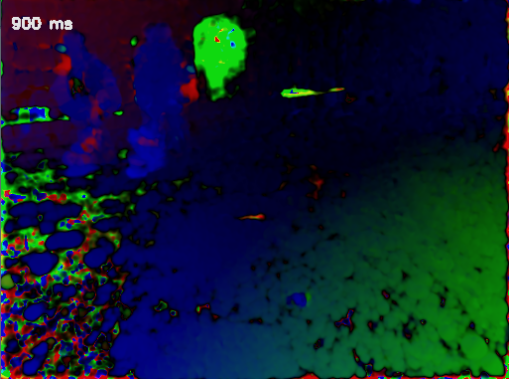
\includegraphics[width=\textwidth]{Chapter3/graphics/OF_Farneback.png}
	\end{subfigure}
	
	\caption{Flux optique dense : méthode de Farneback (implémentation OpenCV). Le code couleur utilisé pour signaler la direction des vecteurs de déplacement est précisé sur la figure \ref{fig:ch3_code_couleur}}
	\label{fig:ch3_OF_Farneback}
\end{figure}

\paragraph{\emph{Graph Cut}:\\}
Les méthodes dites de \emph{Graph Cut} représentent l'espace des solutions possibles comme un graphe, la solution optimale étant alors une section de celui-ci minimisant une fonction de coût. La définition de cette dernière rend possible la prise en compte de contraintes globales dans la recherche d'une solution, le résultat étant très dépendant des paramètres pris en compte. Freedman et al. (\cite{Freedman}) proposent par exemple la détermination du changement global d'illumination a priori, conservant dans la procédure de \og graph cut\fg{} les coûts (ou l'énergie, les formulations peuvent différer) liés à un changement local de luminosité.

D'autres approches sont par ailleurs possibles, notamment en combinant des méthodes locales et globales de calcul du flux optique (par exemple \cite{Bruhn2005} qui combine Horn-Schunk et KLT). Nous n'avons pas retenu ces méthodes pour deux raisons : leur coût en termes de calcul est très important, et les contraintes apportées, si elles permettent le lissage des point aberrants, n'apportent pas réellement d'information supplémentaire. En effet, hors implémentation très agressive et difficilement généralisable dans le domaine de la robotique (\cite{Dumortier} par exemple pour un calcul intégralement sur GPU), le suivi de point dense est encore loin d'être temps réel. Par ailleurs, les différentes contraintes présentées dans les méthodes précédentes permettent d'obtenir une solution globalement améliorée par rapport à une optimisation naïve, mais elles n'offrent aucune garantie d'améliorer les résultats locaux. On constate ainsi aisément sur la figure \ref{fig:ch3_OF_Farneback} que de nombreuses zones de l'image ne sont pas correctement suivies, sans que cette information ne soit immédiatement accessible (certains algorithmes proposent cependant une évaluation intrinsèque de la qualité du suivi). Nous avons finalement choisi de nous concentrer sur le suivi de points saillants, aussi nombreux que possible, mais non denses. Un mécanisme de rejet, obtenu par le cumul de quatre suivis non-corrélés, nous permet enfin de ne conserver que les points fiables.

\section{Algorithme proposé} \label{sec:ch3_Vision_mécanisme}
\subsection{Processus général : Détection et maintien d'un ensemble de points d'intérêt}
Le processus proposé pour l'acquisition des indices visuels, illustré sur la figure \ref{fig:ch3_processus} est superficiellement présenté dans les points suivants. Nous détaillerons ces éléments dans les sections suivantes, on ne présente ici que les principes retenus : \\
\begin{itemize} \renewcommand{\labelitemii}{$\cdot$}
	\item \textbf{Initialisation:} \\ 
	Recherche de points d'intérêt	\\
	
	\item \textbf{Itérations:}
	\begin{enumerate}
		\item Suivi redondant des points sur une paire stéréo
		\item Recherche des points aberrants
		\item Sélection de nouveaux points dans l'image courante:
		\subitem - utilisation d'un masque pour éviter l'accumulation de points sur les zones texturées
		\subitem - tri des meilleurs points obtenus
		\subitem - pression de sélection pour augmenter les points sur une zone privilégiée
	\end{enumerate}
\end{itemize}

\begin{figure}[h]
	\centering
	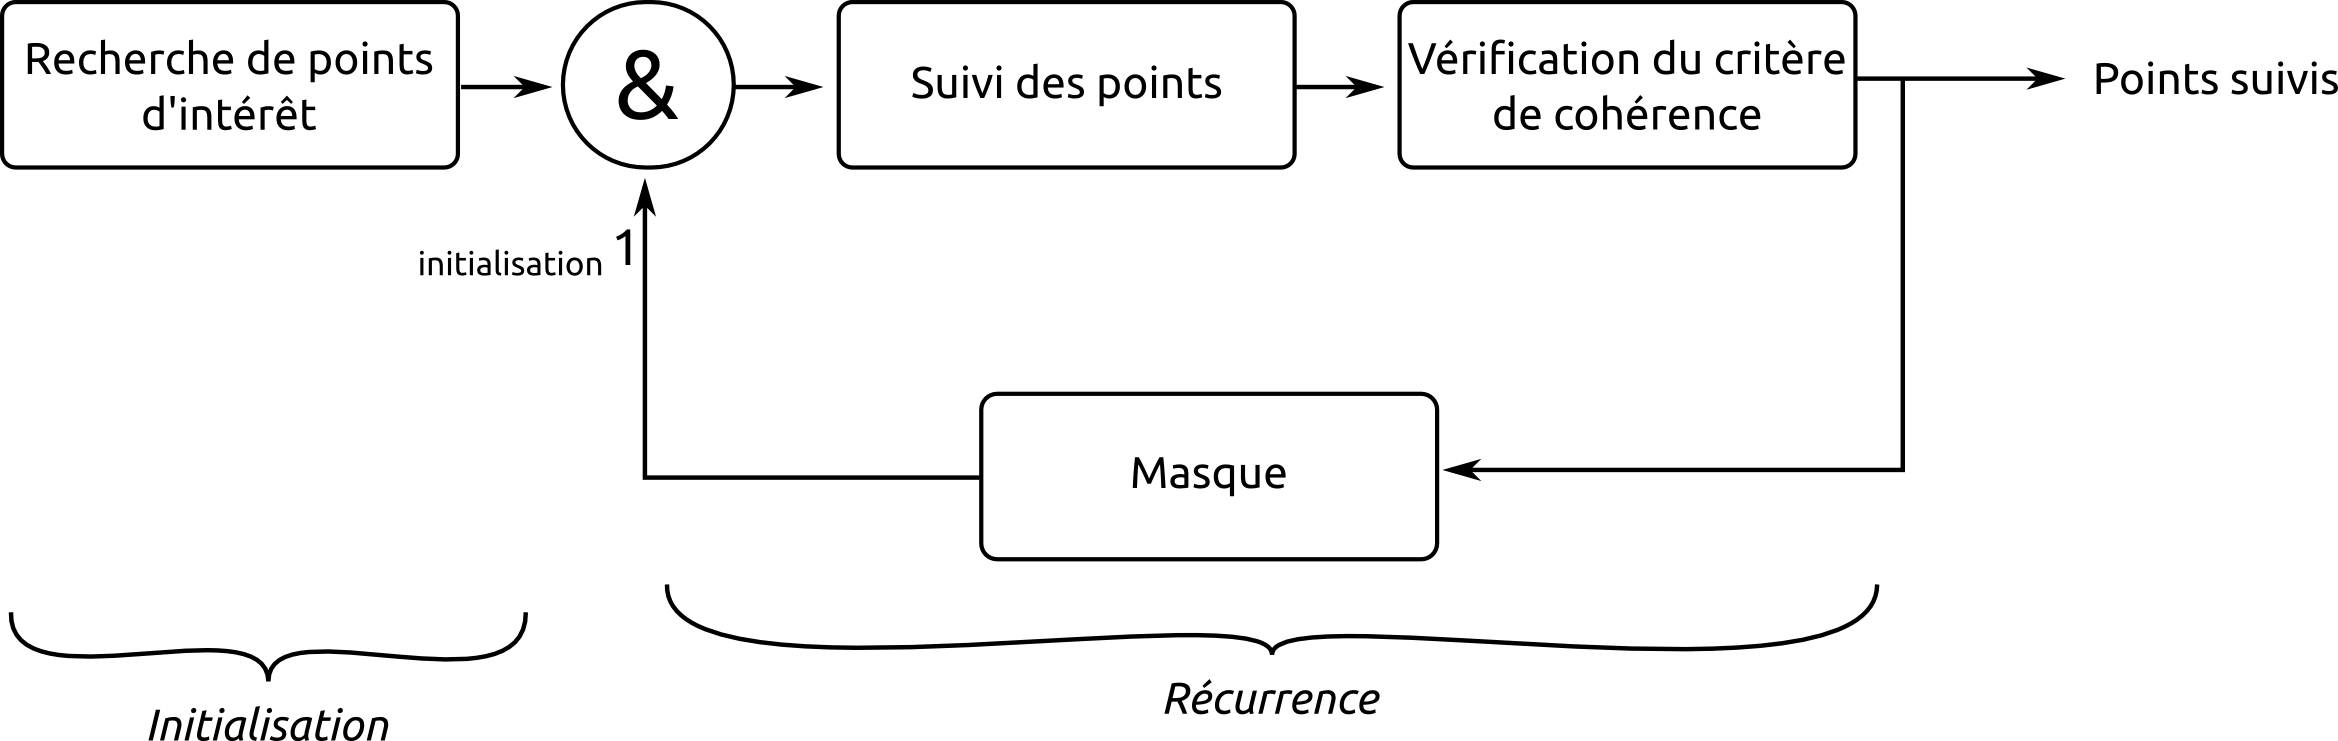
\includegraphics[width=0.9\textwidth]{Chapter3/graphics/tracking_process.png}
	\caption{Processus proposé pour maintenir un ensemble de points suivis}
	\label{fig:ch3_processus}
\end{figure}

Cet algorithme s'applique sur des paires d'images, la vérification de la fiabilité du suivi de points étant réalisée par redondance grâce à un suivi sur des paires d'images et dans le temps. Il vise à maintenir à chaque nouvelle acquisition un ensemble de points suivis représentatifs de l'environnement, et dont la fiabilité est raisonnablement garantie. Des points sont nécessairement perdus lors de chaque nouvelle acquisition, du fait du déplacement du porteur et de la modification de son champ de vision, ce qui rend le processus de ré-introduction de points obligatoire, quel que soit l'algorithme de suivi de points. \\
On essaie de garantir la représentativité de cet ensemble de points selon deux critères : la densité des points doit être localement uniforme, tandis que certaines zones définies comme d'intérêt peuvent être favorisées par rapport à d'autres. On souhaite ainsi être capable de s'affranchir des disparités locales de texture et de contraste, tout en étant capables si besoin d'augmenter la densité locale d'échantillonnage sur les zones perçues comme importantes. 

\subsection{Choix d'un algorithme de suivi de points}
On peut tout d'abord détailler le choix de l'algorithme de suivi de points, parmi les techniques proposées dans la section \ref{sec:ch3_suivi_de_points}.  Comme nous aurons l'occasion de le détailler par la suite, l'un des enjeux de notre méthode consiste à exploiter l'accumulation des observations pour améliorer la position du positionnement des éléments de la scène. Nous souhaitons donc être capables de suivre des éléments visuels sur un laps de temps le plus important possible, idéalement de l'ordre de la fenêtre d'intégration utilisée. Le nombre de points suivis que nous envisageons est par ailleurs relativement important, étant de l'ordre de plusieurs milliers.\\
Nous avons alors considéré que la méthode de suivi de points par re-détection et association était susceptible de perdre un nombre important d'éléments, du fait d'un changement de perspective, ou simplement parce qu'un point initialement parmi les points les plus saillants de l'image n'était plus ensuite suffisamment visible. Cette problématique est notamment abordée par les articles présentant les détecteurs SIFT et SURF, qui se montrent très robustes aux changement de perspective ou d'illumination (\cite{Lowe1999a,Bay}). Cette robustesse ne s'étend cependant pas, dans ces publications fondatrices, aux milliers de points que nous souhaitons suivre. Nous avons donc retenu une technique par optimisation, l'algorithme KLT dans sa version pyramidale (cf. \ref{sec:Annexe_klt}).

\subsection{Suivi redondant sur une paire stéréo} \label{sec:ch3_Suivi redondant}
\subsubsection{Principe}
S'agissant d'acquisitions stéréoscopiques, il est possible de définir une succession de suivis de points non-corrélés, et dont le résultat est déterministe dans un cas optimal. On suit dans ce cas la méthode notamment exploitée par Lategahn et Lenz dans \cite{Lategahn2011, Lenz2011}, en l'appliquant cependant à l'ensemble de nos points d'intérêt et non à quelques points de référence. Cette proposition consiste en l'utilisation conjointe d'un suivi dans le temps et d'un suivi sur les deux images acquises par un ensemble stéréoscopique, en conservant à tout moment la paire d'acquisitions précédentes, comme schématisé par la Figure \ref{fig:ch3_4Frame}.\\

\begin{figure}[h]
	\begin{center}
		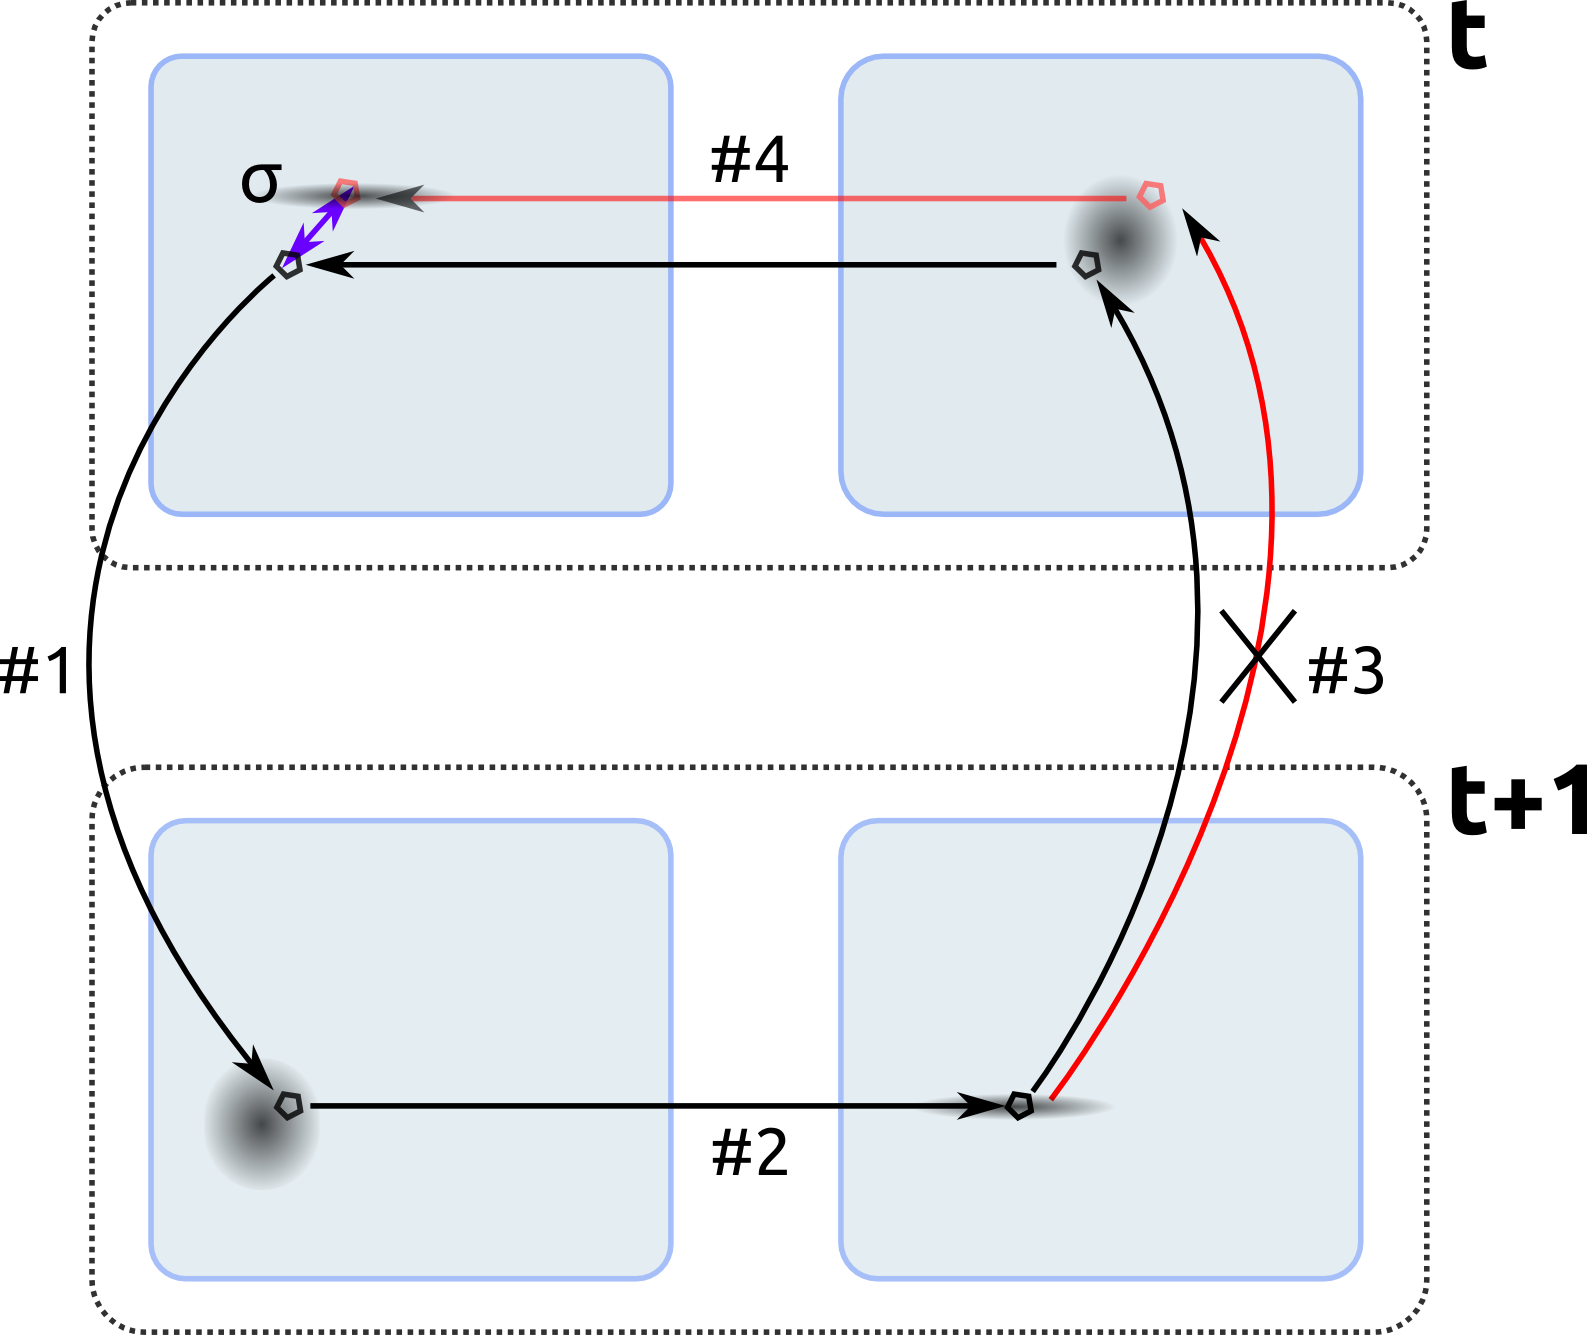
\includegraphics[width=0.5\textwidth]{Chapter3/graphics/4-Frames.png}
	\end{center}	
	\caption{Illustration du processus de suivi redondant de points, et de réjection de points fautifs. Un suivi fautif est illustré en rouge, tandis que les espaces de recherche des différents suivis sont marqués par une zone noircie.}
	\label{fig:ch3_4Frame}
\end{figure}

La Figure \ref{fig:ch3_4Frame}, nous permet par ailleurs d'illustrer les remarques suivantes. Les deux suivis de points dans le temps (étapes 1 et 3) ont un espace de recherche isotrope dans le plan image, tandis que les étapes 2 et 4 sont accélérées par une recherche sur les lignes uniquement. On comprend bien qu'un suivi de point parfait nous conduit à la position initiale, c'est-à-dire que la somme des déplacements calculés par les étapes 1,2,3 et 4 s'annulent. Dans cet exemple, le suivi de point de l'étape 3 est fautif, et nous conduit à l'écart $\sigma$ observé par comparaison entre la position de départ et celle d'arrivée.\\

\subsubsection{Détails de la méthode}
La position initiale des points à suivre est connue, car il s'agit des points correctement suivis à l'étape précédente, auxquels s'ajoutent les points d'intérêt nouvellement introduits. La procédure proposée pour la sélection de ces nouveaux points sera présentée par la suite (cf. \ref{sec:ch3_Sélection des points d'intérêt} et \ref{sec:ch3_Sélection dynamique des points d'intérêt}). On effectue ensuite quatre étapes de suivi de points, chaque étape utilisant la position obtenue lors du suivi précédent. Le critère de qualité final est individuel, il est lié pour chacun des points à la somme des déplacements obtenus lors de son suivi successif sur les 4 étapes proposées. Cette somme doit bien sûr être nulle dans le cas d'un suivi parfait, on fixe en pratique un seuil d'erreur maximal. Cette vérification est par ailleurs combinée au critère de perte de point intrinsèque à l'algorithme KLT (\ref{eq:ch3_KLT_iteration}) : si la matrice $G$ n'est pas inversible (si son déterminant est inférieur à un seuil $min_{det}$), le point est considéré comme perdu. Si l'on note ${d_{i,i+1}}^k$ le déplacement du point $k$ entre les images $i$ et $i+1$, $\sigma^k$ l'erreur mesurée lors de la procédure de suivi, et ${\delta_{i,i+1}}^k$ le statut obtenu après un suivi de point par l'algorithme KLT, on obtient la définition formelle de la validité $V^k$ de notre point :\\
\begin{align}
	\sigma^k 					=& \: \sum\limits_{i=0}^{3} {d_{i,j}}^k  \qquad (j = i+1 \: modulo \: 3)\\
	{\delta_{i,j}}^k :=& \: [ det(G_{i,j} > min_{determinant}] 	\\
	\delta_k 					=& \: \prod\limits_{i=0}^{3} \delta_{i,j}^k 				\\
	V^k 							=& \: [\sigma^k < {\sigma}_{max}] \times \delta_k
\end{align}

On pourra remarquer que la charge de calcul supplémentaire liée à cette procédure, si elle peut sembler considérable, n'est en réalité pas rédhibitoire. Le suivi de points entre les deux caméras est en effet simplifié par la rectification des images, qui permet de ne chercher les correspondances que sur un nombre de ligne limité, méthode souvent utilisée dans le calcul des cartes de disparité. Par ailleurs, l'algorithme KLT s'adapte très bien à cette procédure, dans le sens où les pyramides d'images et leurs gradients n'ont pas à être re-calculés dans le cadre de notre suivi redondant. La charge de calcul supplémentaire est ainsi uniquement liée aux itérations \ref{eq:ch3_KLT_iteration} et \ref{eq:ch3_KLT_pyramid}. Nous montrons dans \ref{sec:ch3_Implémentation} qu'il est possible de réaliser cette opération en temps réel et sur un grand nombre de points (plusieurs milliers) par une implémentation adaptée.

\subsection{Sélection de nouveaux points} \label{sec:ch3_Sélection des points d'intérêt}
\subsubsection{Principe}
La sélection de nouveaux points n'est pas aussi simple qu'un examen rapide pourrait le laisser supposer. L'utilisation d'un détecteur de points d'intérêt est évidemment requise, mais le critère de sélection des points est important. Le tri des points selon leur saillance conduirait ainsi à l'accumulation de points sur les zones les plus contrastées et texturées de l'image, tandis que d'autres zones peuvent rester inobservées. L'uniformité de la densité d'information est un critère important dans notre démarche (voir \ref{sec:ch3_densité informations}), tant on ne peut initialement préjuger des zones les plus porteuses d'informations. Par ailleurs, nous souhaitons pouvoir si besoin augmenter la densité de l'échantillonnage sur certaines zones préalablement identifiées, par exemple par un algorithme ou capteur tiers. \\

On propose finalement la procédure suivante, consécutive à la détection des points d'intérêts de l'image et à même de sélectionner les nouveaux points les plus appropriés :
\begin{itemize}
	\item \textbf{Rejet des points proches de l'existant:\\}
	Création d'un masque autour des points déjà présents, afin d'établir une distance minimale entre deux points suivis. \\
	
	\item \textbf{Sélection préférentielle dans les zones d'intérêt:\\} 
	Création d'un second masque lié aux zones dont on veut améliorer la connaissance. Il s'agit simplement d'évaluer la présence ou non des points testés dans les zones d'intérêt, le nombre de points choisis à l'intérieur et à l'extérieur de ces zones étant décrit par la suite.\\
\end{itemize}

Les nouveaux points sont systématiquement sélectionnés par le premier masque, puis l'utilisation du second masque est décrite dans \ref{sec:ch3_Sélection dynamique des points d'intérêt}. Le seuil de détection des points d'intérêt est volontairement fixé très bas dans notre implémentation, nous permettant de \og saturer\fg{} ce mécanisme de sélection. Ceci conduit cependant à des calculs inutiles, et un mécanisme de seuil adaptatif serait sans doute préférable.

\subsubsection{Intérêt de l'utilisation de masques}
En notant $N_{initiaux}$ le nombre de points présents initialement, et $N_{nouveaux}$ le nombre de points à introduire, avec $N_{initiaux} >> N_{nouveaux}$, l'intérêt d'une implémentation par masque peut se décrire en termes de complexité. L'ordre de grandeur des opérations à effectuer pour trier les points selon les critères précédents est en effet de $O(N_{initiaux} \cdot N_{nouveaux})$ pour une implémentation naïve par comparaison directe, contre $O(N_{nouveaux} + N_{initiaux})$ pour une implémentation par masque de réjection.\\

Il est à noter qu'une approche différente, à base d'arbres quaternaires (\emph{Quadtrees}), est également proposée par Mei et al. (\cite{Mei2010, Mei}) pour favoriser l'homogénéité des points sur l'image. Cette technique est couramment utilisée pour segmenter l'espace, une surface donnée pouvant être successivement subdivisée en 4 cellules indexées dans un arbre de décision, chaque feuille ayant dans ce cas 4 enfants, jusqu'à ce que la subdivision soit suffisamment petite. Dans leur approche, la répartition des points est explicitement uniforme à grande échelle, puis forcée à tous les étages de l'arbre tant que la détection de points d'intérêt dans la cellule désignée est concluante. \\
Cet algorithme se prête cependant mal à une distribution volontairement non-uniforme des points, comme nous le proposons ci-dessous, et nous avons supposé que ces deux approches étaient par ailleurs équivalentes en termes de rapidité d'exécution. On accepte cependant, avec notre implémentation, une perte d'uniformité qui nous conduit à favoriser les points d'intérêts de meilleure qualité.

\subsubsection{Mécanisme de sélection préférentielle des nouveaux points} \label{sec:ch3_Sélection dynamique des points d'intérêt}
Supposons ici que l'on veuille modifier dynamiquement la densité d'échantillonnage des points sur une image, en l'augmentant sur des zones distinctes d'un rapport $k$. On peut alors décrire un mécanisme permettant de tendre vers cette répartition grâce à une sélection adéquate de nouveaux points. On note pour ce faire $N_o^l$ le nombre de points à l'extérieur de la zone privilégiée lors de l'itération $l$, et $N_t^l$ le nombre de points à l'intérieur de cette zone visée lors de l'itération $l$. On note de même $S_o^l$ et $S_t^l$ les surfaces respectives des zones neutres et visées. On note enfin  $N_{o,i}^l$ (respectivement $N_{t,i}^l$) le nombre de points à introduire dans la zone neutre (respectivement visée) lors de l'itération $l$. On souhaite alors tendre vers $d_t = k \cdot d_o$ avec $d$ la densité d'information échantillonnée par unité de surface. 

\begin{align}
	d_t^{l+1} =& \: k \cdot d_o^{l+1} \\
	\frac{N_t^l + N_{t,i}^{l+1} }{S_t^{l+1}} =& \: k \cdot \frac{N_o^l + N_{o,i}^{l+1} }{S_o^{l+1}} \\
	N_{t,i}^{l+1} =& \: S_t^{l+1} \cdot k \cdot \frac{N_o^l + N_{o,i}^{l+1} }{S_o^{l+1}} - N_t^l 
\end{align}

Connaissant par ailleurs le nombre total de nouveaux points à introduire $N_i^{l+1} = N_{o,i}^{l+1} + N_{t,i}^{l+1}$ on obtient simplement :

\begin{align}
	N_{t,i}^{l+1} &= \:\frac{k \cdot \frac{S_t^{l+1}}{S_o^{l+1}} \cdot (N_o^l + N_i^{l+1}) - N_t^l}  {1 + k \cdot \frac{S_t^{l+1}}{S_o^{l+1}}} \\
	N_{o,i}^{l+1} = \: N_i^{l+1} - N_{t,i}^{l+1} &= \frac{ N_i^{l+1} + N_t^l - k \cdot \frac{S_t^{l+1}}{S_o^{l+1}} \cdot (N_o^l + N_i^{l+1})}  {1 + k \cdot \frac{S_t^{l+1}}{S_o^{l+1}}}
\end{align}

On a supposé dans le calcul précédent que nous disposions de suffisamment de points détectés pour satisfaire l'ensemble des contraintes ($N_{o,i}^{l+1}$ et $N_{t,i}^{l+1}$ sont saturables, c'est-à-dire que l'on a détecté suffisamment de points pour les ajouts effectifs soient ceux prévus par l'algorithme). Dans le cas contraire, on fait le choix de ne pas respecter la répartition demandée afin de privilégier le renouvellement des points perdus par rapport à leur répartition dans l'image. On ne propose donc pas un algorithme déterministe, mais une \og pression de sélection\fg{} quant à l'ajout de nouveaux points qui doit nous permettre de tendre vers une répartition souhaitée. \\

Dans le cas où les points détectés seraient trop nombreux (relativement à un seuil arbitraire, fixé à 5000 points dans notre implémentation), on exploite tout d'abord un mécanisme dit de "<sélection par tas\fg{} (\emph{heap select}), similaire au "<tri par tas\fg{} sans produire toutefois de sélection triée. Le critère de qualité utilisé pour la sélection est la réponse au détecteur de points d'intérêt, qui varie selon les méthodes (cf. section \ref{sec:ch3_Détection_points_intérêt}).\\

Un exemple de résultat est visible sur la Figure \ref{fig:ch3_Weighted_selection}, dans laquelle le rapport de densité demandé entre l'intérieur et l'extérieur de la ROI (\emph{Region Of Interest }, zone d'intérêt) est inférieur à 1. On souhaite donc éviter d'échantillonner cette zone, ce qui pourrait par exemple correspondre au suivi d'un véhicule dont la position est connue. On constate bien que la densité des points est très inférieure à l'intérieur de la zone d'exclusion, comme souhaité. \\

La complexité de ce mécanisme de sélection n'est que marginalement augmentée par rapport à l'usage d'un masque simple qui évite l'accumulation, et reste de l'ordre de $O(N_{nouveaux} + N_{initiaux})$.

\begin{figure}[h]
	\begin{center}
		\begin{subfigure}{0.58\textwidth}
		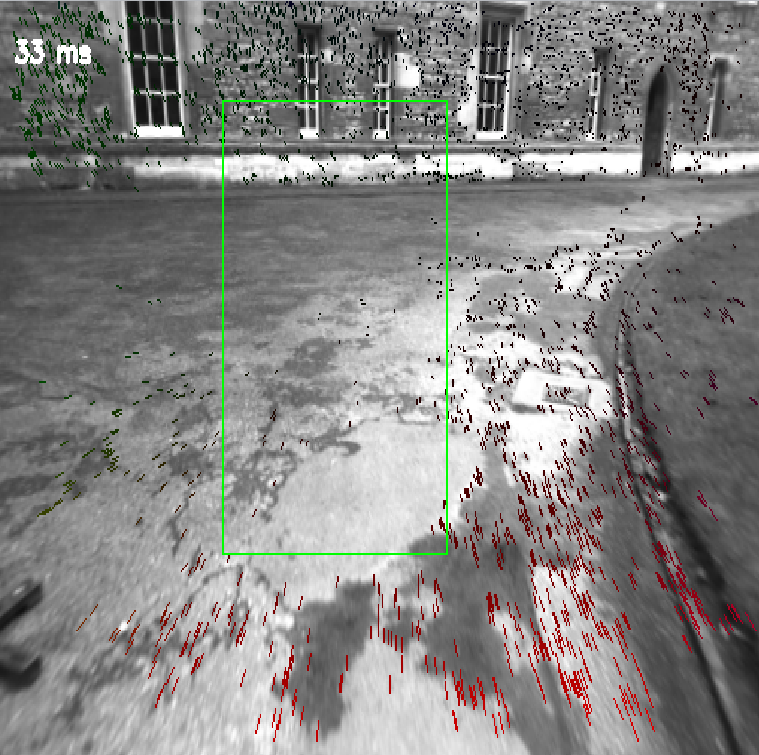
\includegraphics[width=\textwidth]{Chapter3/graphics/Detectors_weighted.png}
		\caption{La zone délimitée en vert correspond à une densité souhaitée plus faible.}
		\end{subfigure}	
		~
		\begin{subfigure}{0.38\textwidth}
			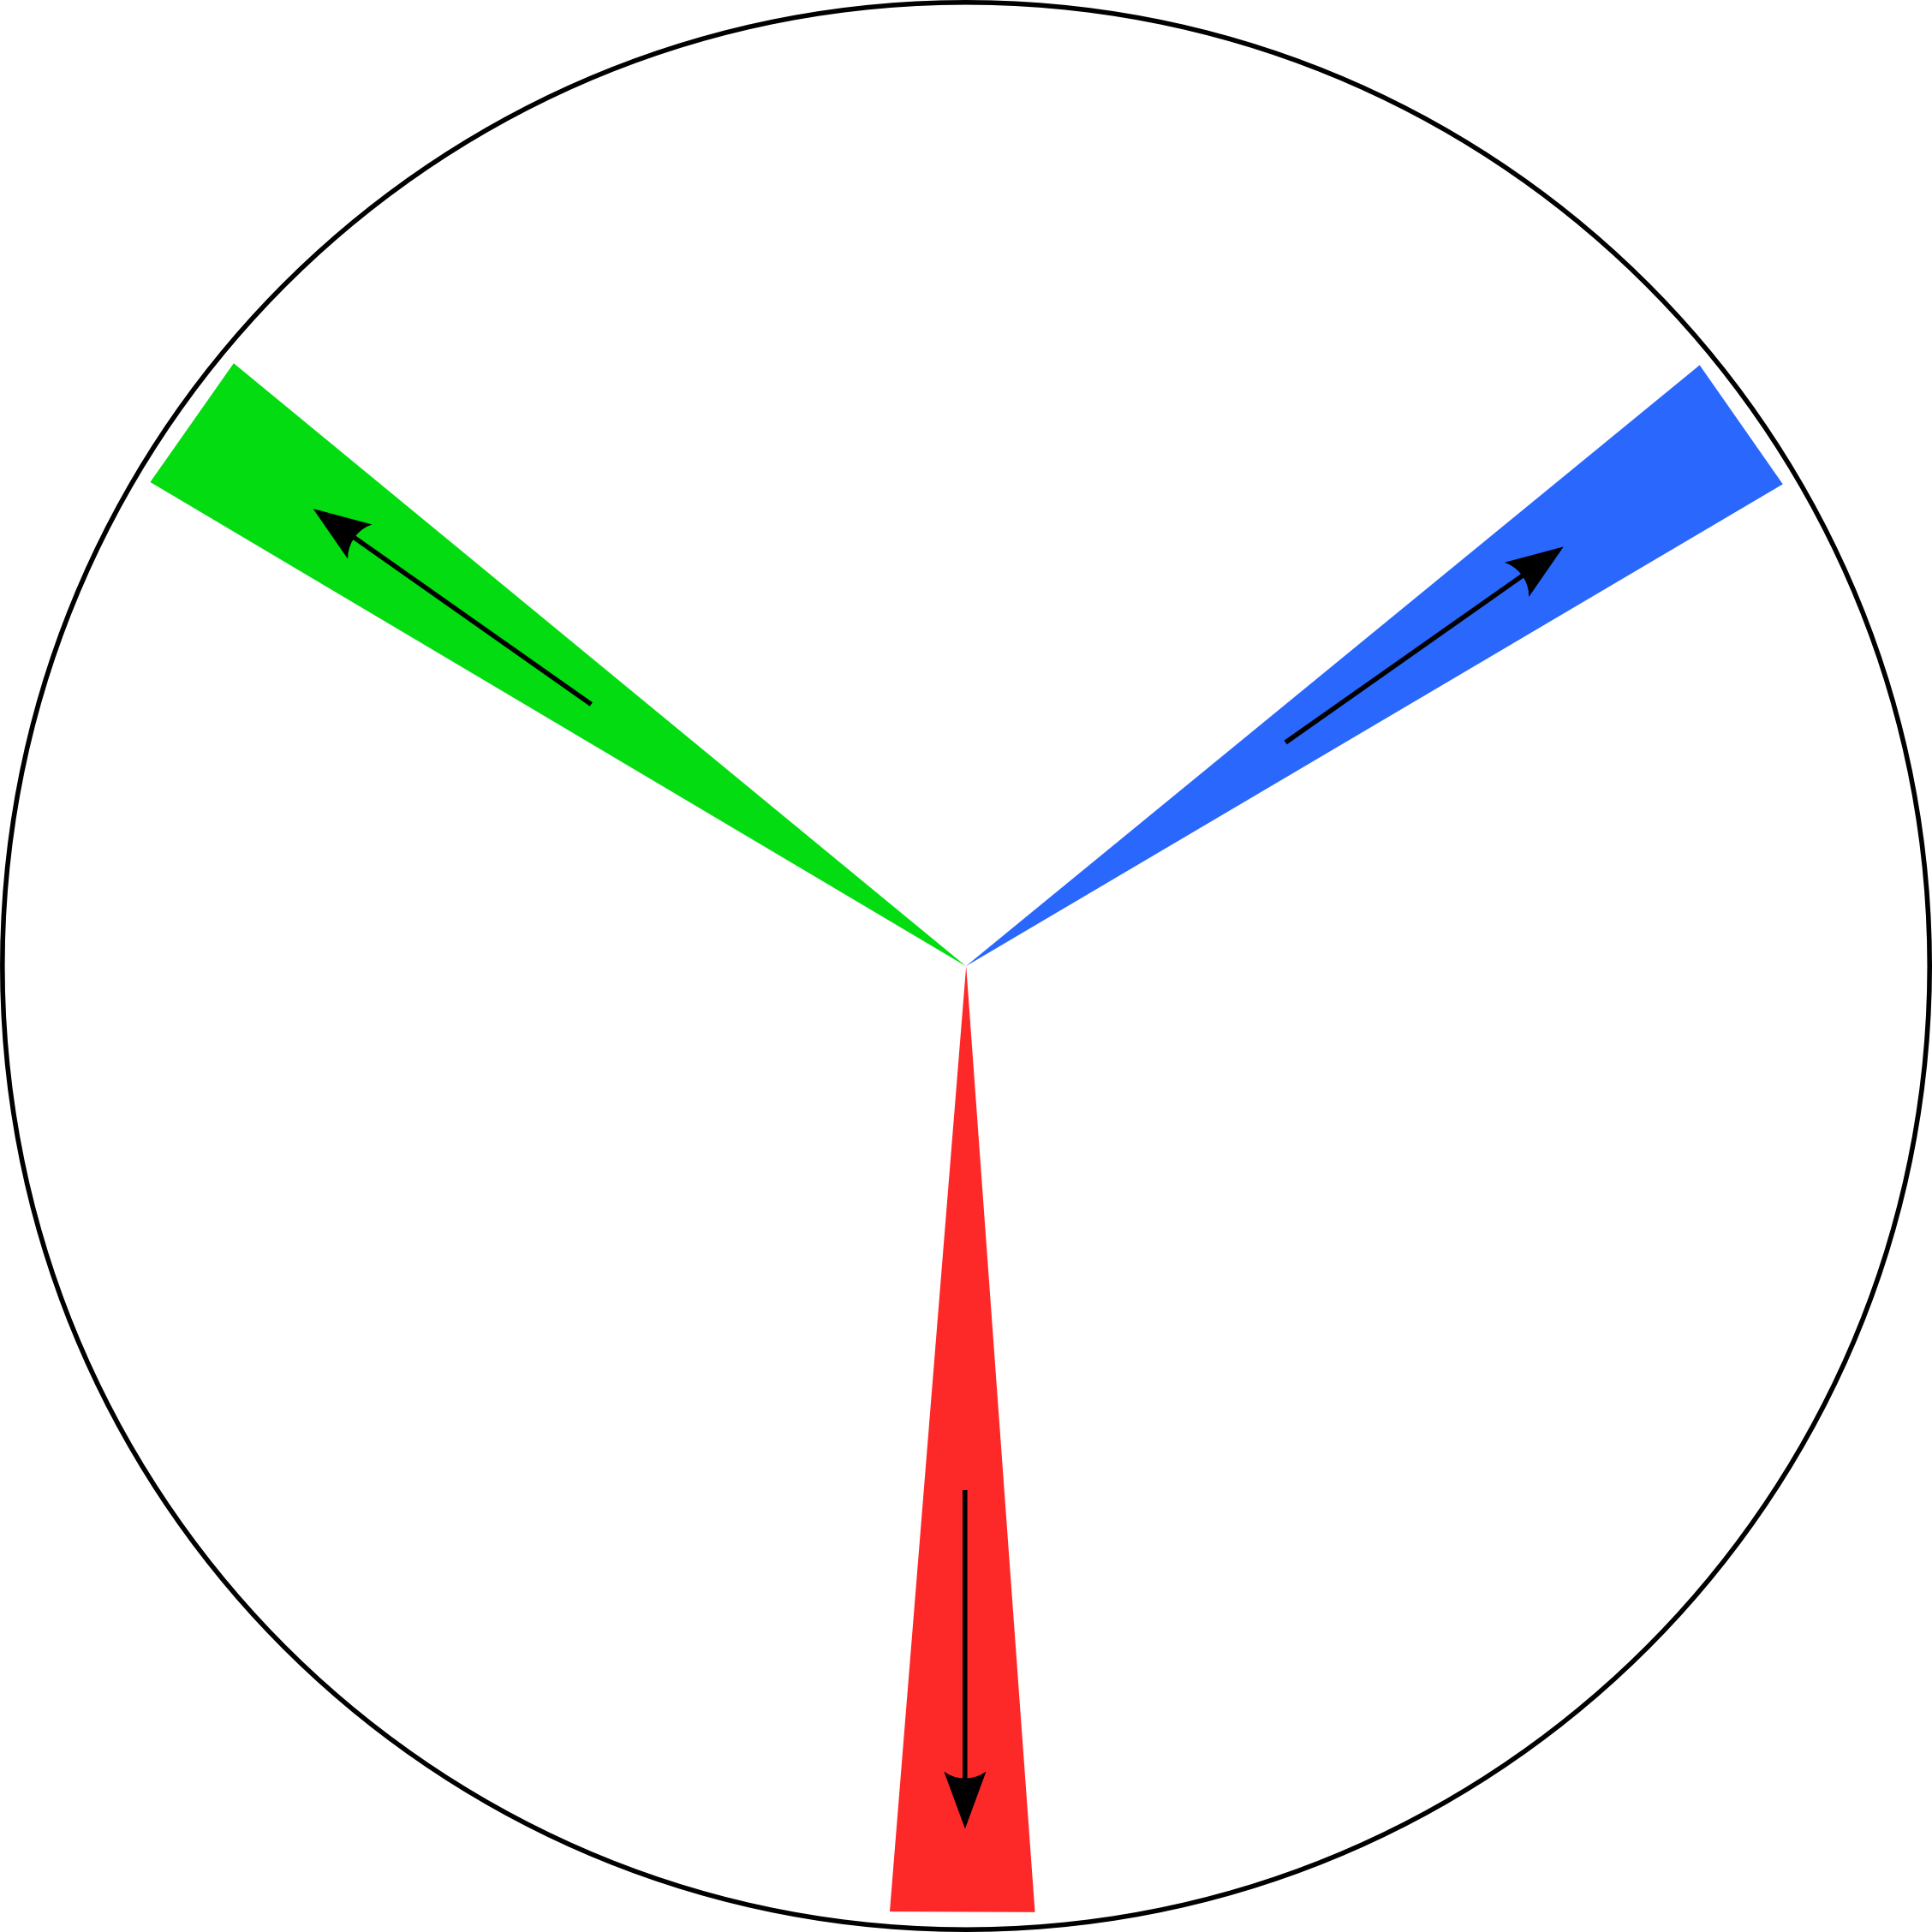
\includegraphics[width=\textwidth]{Chapter3/graphics/directions_chroma.png} 
			\caption{Code couleur représentant les directions des vecteurs de déplacement dans le plan image}
			\label{fig:ch3_code_couleur}
		\end{subfigure}	
	\end{center}
	\caption{Exemple de résultat de l'algorithme de sélection préférentielle des nouveaux points d'intérêt}	
	\label{fig:ch3_Weighted_selection}
\end{figure}

\section{Implémentation et évaluation}
\subsection{Détection de points d'intérêt}\label{sec:ch3_Eval_PI}
Comme abordé dans \ref{sec:ch3_Détection_points_intérêt}, de nombreux détecteurs de points d'intérêt sont présents dans la littérature, et la recherche d'un algorithme les surpassant n'était pas l'objet de cette thèse. Nous avons cependant comparé quelques uns des détecteurs les plus utilisés dans la littérature, par rapport à nos besoins. Trois critères nous semblent en effet importants dans notre perspective d'un traitement temps réel sur de nombreux points suivis dans le temps : 
\begin{itemize}
	\item le nombre de points détectés doit être important pour justifier notre démarche, supérieur à 4000 points en pratique,.
	\item le temps de détection doit être le plus faible possible, cette opération étant renouvelée à chaque itération,
	\item la qualité des points sélectionnés doit être la plus grande possible, dans le sens ou le suivi de points redondant mis en place (\ref{sec:ch3_Suivi redondant}) doit permettre de conserver le plus de points possibles d'une itération sur l'autre tout en conservant une couverture la plus homogène possible.
\end{itemize}

Le premier point ici soulevé n'est pas discriminant : chacun des détecteurs envisagés est associé à un seuil de détection, et l'ajustement de celui-ci autorise en pratique, dans tous les cas, suffisamment de nouveaux points. On évalue donc dans ce qui suit les deux points suivants. La séquence utilisée est tirée de la banque de données \textit{New College} (\cite{Smith2009}), acquise par des caméras stéréoscopiques \textit{Point Grey Lady Bug 2}. Ces images ont une taille de 512 x 384 pixels, en niveaux de gris, sur une profondeur de 8 bits.

\subsubsection{Comparaison: temps de calcul}
On compare dans le tableau \ref{tab:ch4_temps_de_calcul} le temps de calcul lié à l'usage des détecteurs Harris, SIFT, SURF, \og Shi et Tomasi\fg{} et FAST sur une séquence d'images. Leurs seuils respectifs autorisent une détection de plus de 4000 points par image. On compare à la fois le temps lié à la détection de points d'intérêt et le temps lié au suivi de points, pour éventuellement prendre en compte un problème lié à une détection de points moins efficace mais plus rapide dans l'absolue dans le cadre de l'algorithme KLT. Le suivi des points est ici confié à une implémentation pyramidale de l'algorithme KLT, exécutée sur le CPU. Les temps de calcul correspondent à une implémentation en C++ exploitant la libraire OpenCV, sur un processeur Core i7 2GHz. On vérifie la constance du temps de détection et de suivi de points sur 300 images, les variations relatives de temps de calcul étant faibles on ne présente ici que les temps moyens. \\

\begin{table}[H]	
	\begin{center}
			\begin{tabular}{| c | c | c | c |} 
				\hline
				Détecteur 					& \pbox[c]{3cm}{\centering {Temps de \newline détection (ms)}} & \pbox[c]{3cm}{\centering {Temps du suivi \newline (ms)}} & \pbox[c]{3cm}{\centering {Temps total \newline (ms)}}\\
				\hline
				\textnormal{FAST}						& 6 	&	54	& 60 	\\
				\hline
				\textnormal{Harris} 				& 10 	&	50	& 60 	\\
				\hline
				\textnormal{Shi \& Tomasi} 	& 11 	&	50	& 61 	\\	
				\hline
				\textnormal{SURF} 					& 33 	&	59	& 91 	\\	
				\hline
				\textnormal{SIFT} 					& 74 	&	54	& 128	\\ 
				\hline
			\end{tabular} 
	\end{center}
	\caption{Comparaison des temps de calcul liés à différentes méthodes de détection, pour 4000 points suivis.}
	\label{tab:ch4_temps_de_calcul}
\end{table}

On constate aisément sur le tableau \ref{tab:ch4_temps_de_calcul} que le temps de calcul lié à l'utilisation des détecteurs SURF et SIFT est rédhibitoire. On n'extrait pas pour ces derniers de descripteur associé, ce qui est par ailleurs une caractéristique recherchée de ces algorithme. Le détecteur FAST est le plus rapide avec une moyenne de 6 ms par frame, suivi par les détecteurs Harris et \og Shi et Tomasi\fg{}. L'intégration de l'étape de suivi de points permet de ramener ces trois derniers algorithmes à une quasi-équivalence. L'algorithme KLT n'offre en effet pas un temps de calcul constant, les critères d'arrêt (outre le nombre maximal d'itérations) étant la stabilisation de la convergence et une matrice G non-inversible.

\subsubsection{Comparaison: qualité}
\paragraph{Perte des points lors du suivi\\}
On compare maintenant la qualité des détections, dans le cadre de nos besoins particuliers. On commence par mesurer pour cela le nombre de points perdus par itération, selon notre critère de cohérence présenté dans \ref{sec:ch3_Suivi redondant}. La tolérance est ici fixée à $\sigma_{max}$ = 1,5 pixel. On peut remarquer que des points sont nécessairement perdus dans cette procédure, la caméra se déplaçant pendant la séquence et modifiant donc son champ de vision. Le nombre total de point suivi dans ce test est de 4000 points.

\begin{figure}[h]
	\centerline{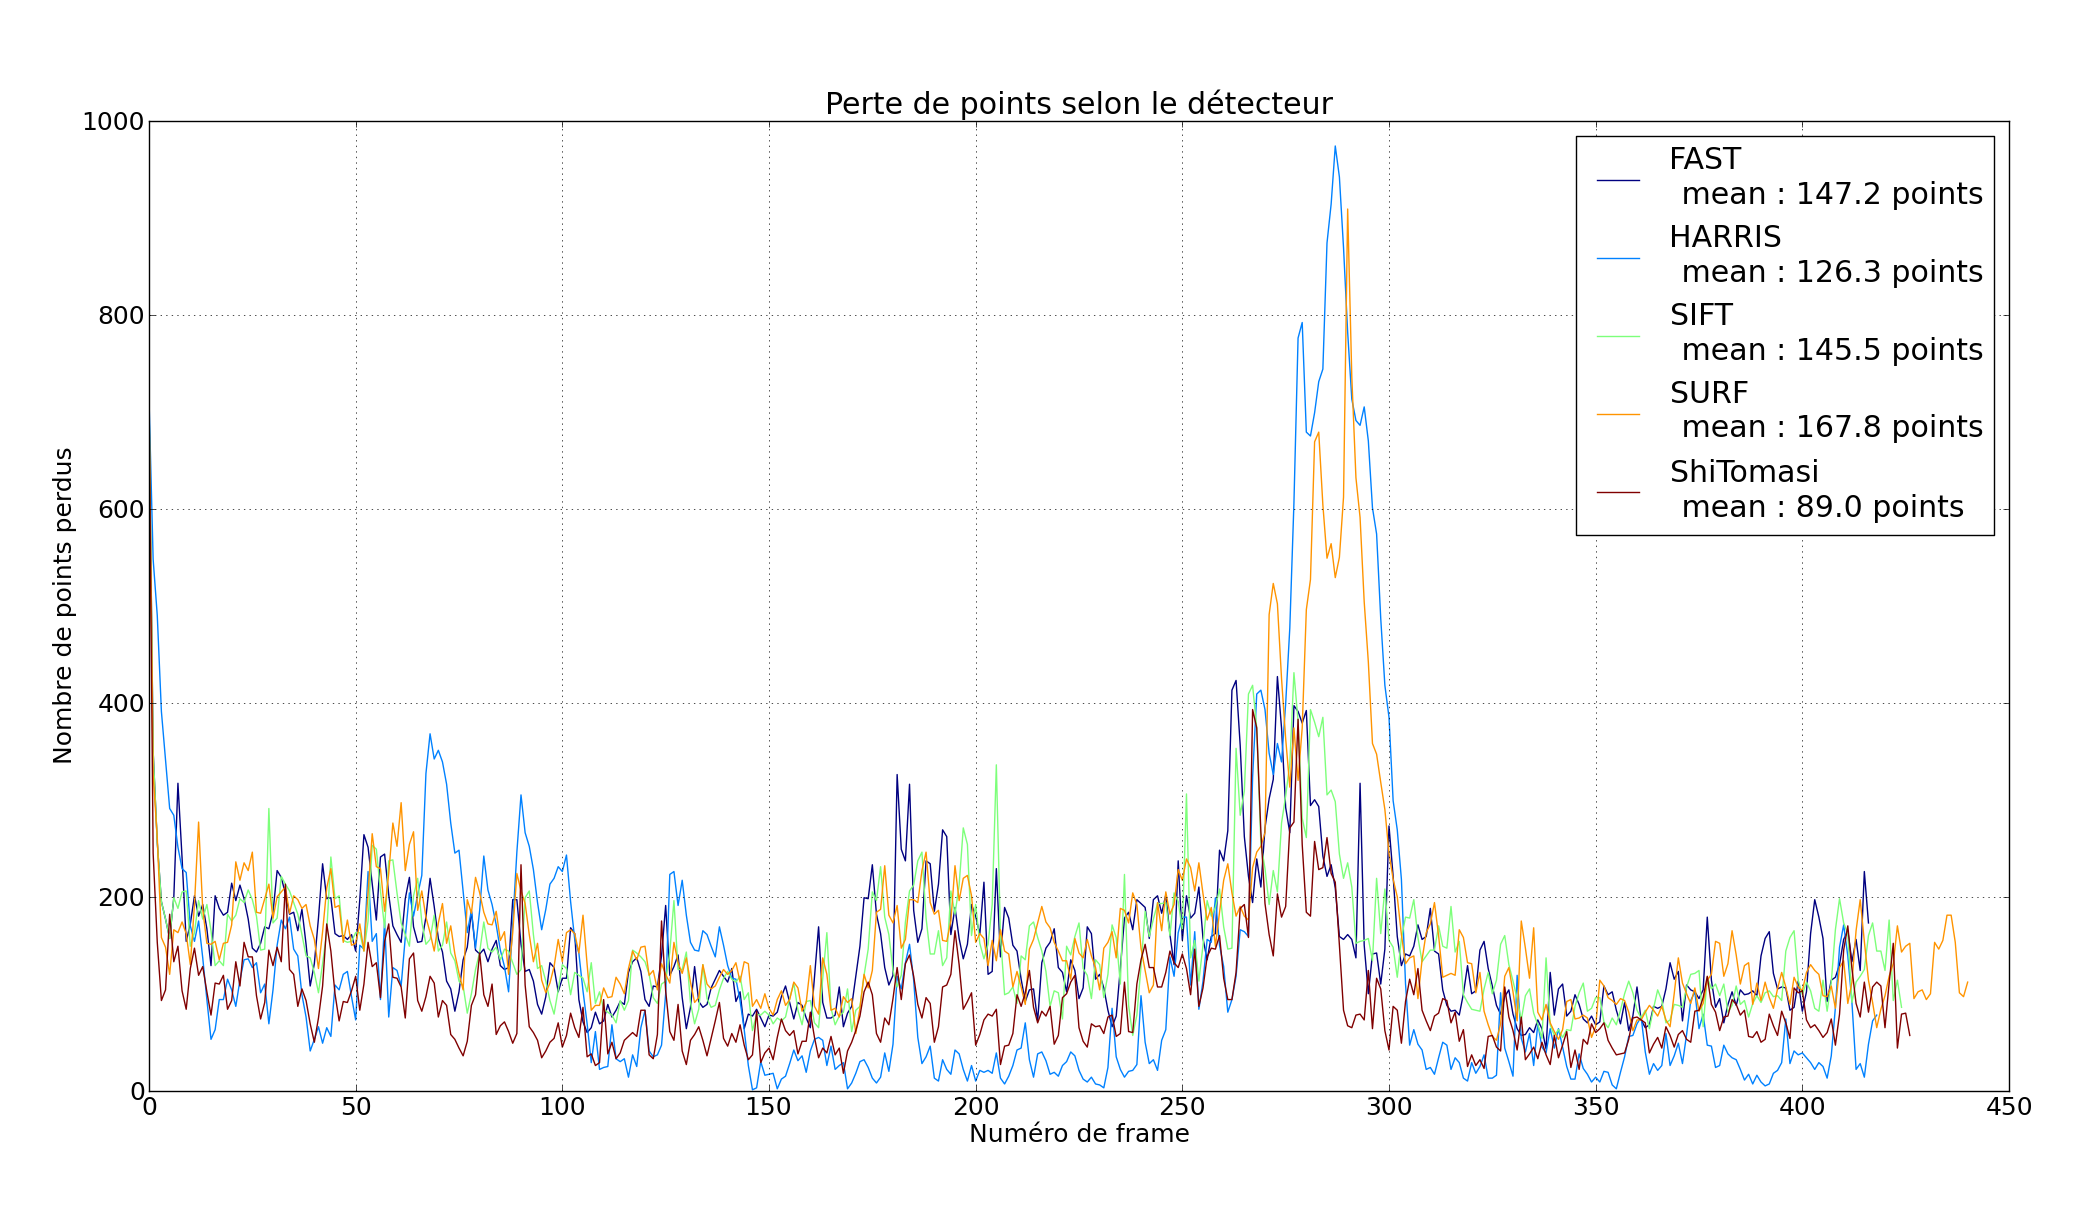
\includegraphics[width=\textwidth]{Chapter3/graphics/Detectors_comparison_q_clean.png}}
	\caption{Comparaison de la qualité des points suivis : évolution du nombre de points perdus pour 5 détecteurs : FAST, Harris, SIFT, SURF et Shi et Tomasi. Les meilleures performances sont obtenues par Shi et Tomasi.}
	\label{fig:ch3_Vision_robustesse}
\end{figure}

La Figure \ref{fig:ch3_Vision_robustesse} nous montre que tous les détecteurs ne fournissent pas des points aussi robustes dans le cadre de notre procédure de suivi par KLT. Les points obtenus par Shi et Tomasi ainsi que les points de Harris occasionnent le moins d'erreur de suivi. On peut par ailleurs constater que le nombre de points perdus peut évoluer de manière significative au cours du temps, du fait des mouvements de la caméra, ce qui met l'accent sur un processus de redistribution des points efficace.

\paragraph{Uniformité\\} \label{Vision_uniformité}
Le nombre de points perdus par itération ne rend cependant pas compte de l'ensemble de nos besoins, l'uniformité de la couverture étant par ailleurs un aspect important. Cette couverture de la scène par les points échantillonnés ne dépend pas seulement de la détection initiale, mais également de la qualité des points détectés, dans la mesure où le suivi des points dans le temps peut modifier cette répartition. On peut constater en comparant la répartition de la population de points suivis (Figure \ref{fig:ch3_Vision_uniformité}), suite à l'usage de deux détecteurs spécifiques pendant un grand nombre d'itérations, que celle-ci diffère grandement quand bien même le reste de l'algorithme est conservé (notamment le rejet par masque des nouveaux points trop proches des points existant, cf. section \ref{sec:ch3_Vision_mécanisme}).

\begin{figure}[h]
	\begin{center}
		\begin{subfigure}{0.48\textwidth}
			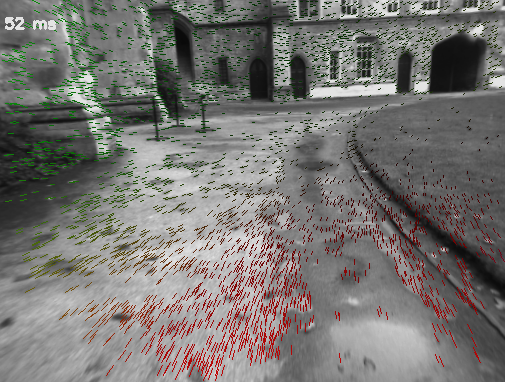
\includegraphics[width=\textwidth]{Chapter3/graphics/Detectors_FAST_init.png} 
			\caption{Détecteur FAST - première détection}
		\end{subfigure}	
		~	
		\begin{subfigure}{0.48\textwidth}
			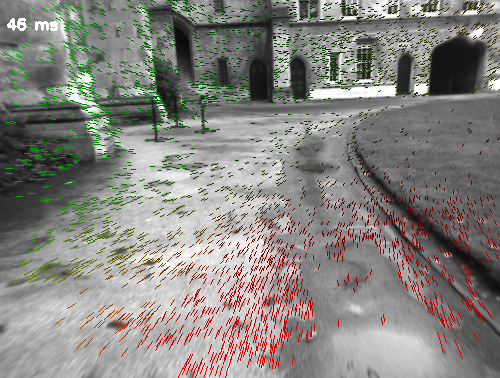
\includegraphics[width=\textwidth]{Chapter3/graphics/Detectors_HARRIS_init.png} 
			\caption{Détecteur Harris - première détection}
		\end{subfigure}
		\\
		\begin{subfigure}{0.48\textwidth}
			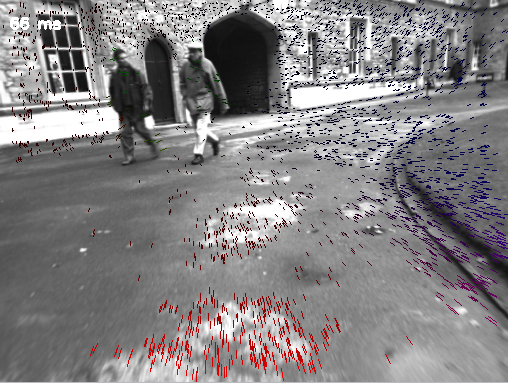
\includegraphics[width=\textwidth]{Chapter3/graphics/Detectors_FAST.png} 
			\caption{Détecteur FAST - 300 itérations}
		\end{subfigure}
		~
		\begin{subfigure}{0.48\textwidth}
			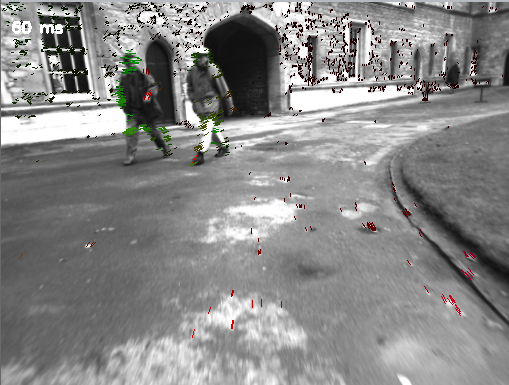
\includegraphics[width=\textwidth]{Chapter3/graphics/Detectors_HARRIS.png}
			 \caption{Détecteur Harris - 300 itérations}
		\end{subfigure}
		
		\caption{Comparaison de la qualité des points suivis : répartition des points après 300 itérations.}	
		\label{fig:ch3_Vision_uniformité}
	\end{center}
\end{figure}

L'explication de cette différence entre ces deux détecteurs est liée aux caractéristiques des points d'intérêt retenus (qui diffèrent grandement selon les détecteurs, comme nous l'avons vu dans \ref{sec:ch3_Détection_points_intérêt}), et à la tolérance accordée au suivi redondant des points (\ref{sec:ch3_Suivi redondant}). Les points détectés peuvent ainsi dériver au fil des itérations du fait de l'imperfection de l'étape de suivi dans le temps, et éventuellement converger vers les mêmes localisations, ce qui contrarie notre ambition d'une couverture angulaire maximale et uniforme. Ce phénomène est patent sur les images de la Figure \ref{fig:ch3_Vision_uniformité}, dans laquelle (dans le cas de l'utilisation de Harris) les points ont \og glissé\fg{} le long des arrêtes. On propose donc de quantifier l'uniformité de la répartition des points par l'étude du nombre de points par unité de surface, sur un pas suffisamment faible pour mettre en valeur les discontinuité de densité. \\
On représente sur la figure \ref{fig:ch3_Vision_densité} la fonction de répartition des points sur l'image en fonction de leur densité locale, avec le procédé suivant : chacun des éléments de surface de l'image (que l'on choisit suffisamment petit) peut recevoir un ou plusieurs points d'intérêt. On représente sur l'axe des abscisses la densité (croissante) de ces éléments de surface, tandis que l'axe des ordonnées représente le nombre de points présents dans des éléments de surface recevant cette densité de points. L'unité élémentaire de surface est choisie par rapport au nombre de points dans l'image, de sorte que théoriquement \textit{chaque unité de surface doit recevoir un unique point d'intérêt en cas de répartition uniforme}. Une distribution plus uniforme est donc plus présente sur la gauche du graphique. Autrement dit, l'axe des abscisses représente le degré de non-uniformité de la fonction de répartition. Cette étude est réalisée après 300 itérations, pour se placer en régime stabilisé, on utilise là encore les données de New College (\cite{Smith2009}).

\begin{figure}[H]
	\centering
	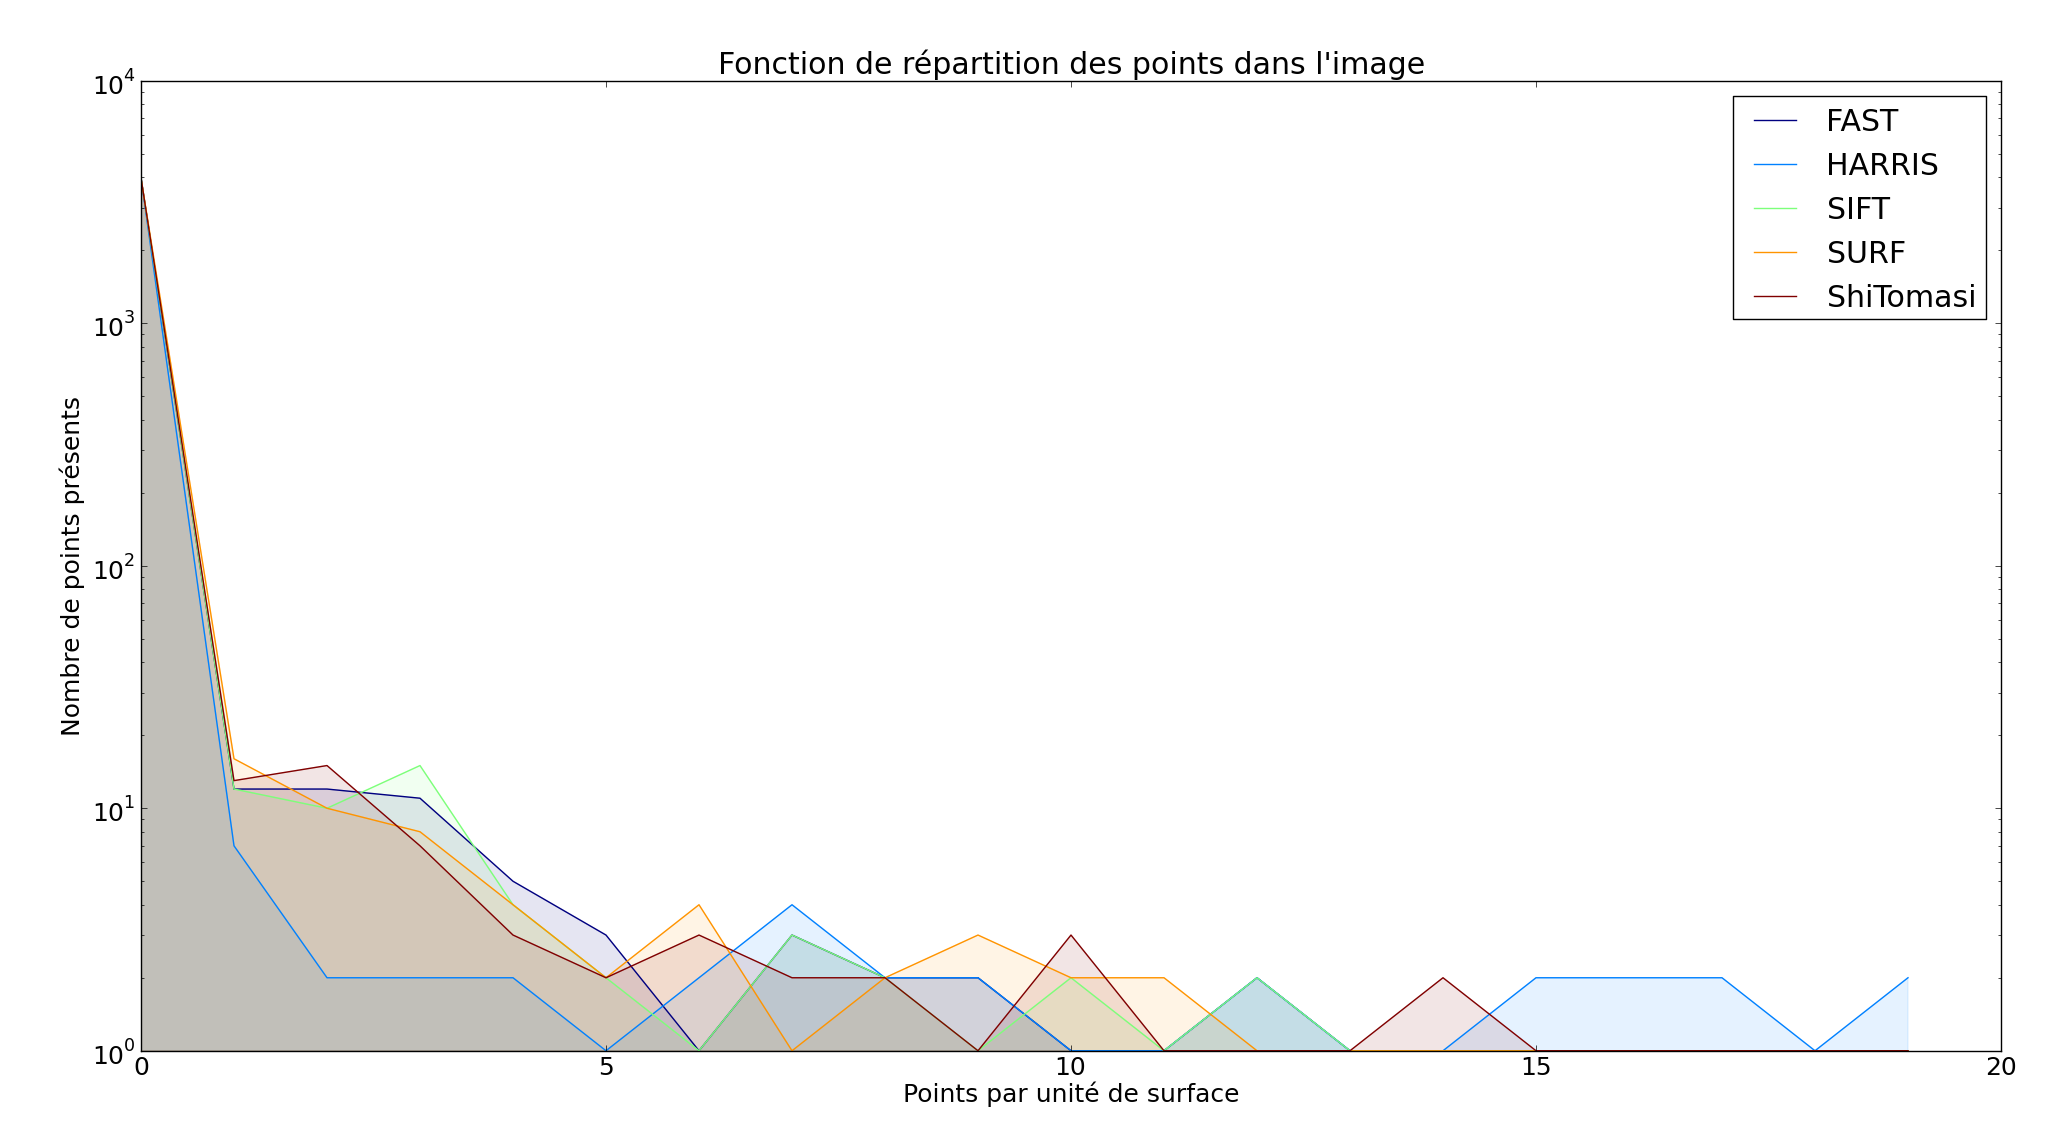
\includegraphics[width=\textwidth]{Chapter3/graphics/Detectors_comparison_density.png}
	\caption{Répartition des points après 300 itérations : mesure de l'uniformité du nombre de points par unité de surface}
	\label{fig:ch3_Vision_densité}
\end{figure}

On constate sur la figure \ref{fig:ch3_Vision_densité} que les points de Harris conduisent effectivement à une répartition moins uniforme. Les points SIFT et SURF sont par ailleurs marginalement meilleurs que les points FAST et Shi et Tomasi, ce qui tend à montrer que les points sélectionnés par ces détecteurs dérivent moins. Cette étude ne vaut bien sûr que pour des points suivis dans le temps par la méthode proposée par Lucas et Kanade, les conclusions pourraient être différentes avec une autre méthode de suivi. \\

\paragraph{Choix du détecteur:\\}
Au vu des évaluations réalisées pour ces différents détecteurs, il nous apparaît que les détecteurs SIFT et SURF, bien que de qualité, sont trop coûteux pour une implémentation visant un traitement temps réel. Les points de Harris, bien que rapides à détecter, se révèlent difficiles à suivre sur une séquence d'images, et contredisent notre effort initial visant à une couverture la plus complète possible du champ de vision. Les points FAST et ceux proposés par Shi et Tomasi nous semblent tous deux convenir au vu de ces évaluations, les second étant cependant plus adaptés au suivi de points par KLT. Il s'agit par conséquent des points que nous avons retenu pour la suite de notre implémentation.

\subsection{Suivi de points} \label{sec:ch3_Implémentation}
Le mécanisme proposé dans ce manuscrit pour le suivi de points, s'il n'est pas nouveau (il est notamment utilisé dans \cite{Lategahn2011} pour le suivi des points utilisés dans la détermination de l'ego-motion, ou dans \cite{Lenz2011}), n'a à notre connaissance jamais été mis en œuvre pour le suivi de l'intégralité des points d'intérêt considérés, sans doute du fait des contraintes associées au temps de calcul.\\
On peut dissocier schématiquement, du point de vue du suivi de points dans une approche de stéréo-vision, l'acquisition d'informations temporelles et spatiales selon que l'on considère les paires intra ou inter-caméras du schéma \ref{sec:ch3_Suivi redondant}. Lategahn propose ainsi un sous échantillonnage des mesures dans le temps (dans le sens où peu de points sont suivis dans le temps) pour mieux densifier la perception de l'environnement (la carte de disparité est calculée de manière dense). Cette méthode autorise la reconstruction d'un environnement très dense, mais se prive par la même de la perception d'un environnement mobile. Les méthodes présentes dans la littérature comportent le plus souvent ce compromis : seuls quelques points sont suivis sur l'ensemble du parcours redondant possible, tandis qu'un suivi dense est réalisé entre les caméras (carte de profondeur dense, par exemple \cite{Agrawal2007}) ou dans le temps (flux optique dense, par exemple \cite{Dumortier}).\\
La perception des objets en mouvement étant l'une de nos priorités, nous avons fait le choix de suivre autant de points dans le temps qu'entre les deux caméras, afin que le nuage de points obtenu puisse être indifféremment composé de points mobiles. Ceci peut poser des problèmes de performances, le temps de traitement d'une telle méthode étant potentiellement incompatible avec une exécution en temps réel. Nous avons donc évalué plusieurs approches pour tenter d'y remédier, et présentons ci-dessous quelques uns des résultats obtenus.

\subsubsection{Implémentation OpenCV}
Le mécanisme décrit dans \ref{sec:ch3_Suivi redondant} est assez simplement réalisable en utilisant les algorithmes disponibles dans la librairie OpenCV. Une implémentation naïve, utilisant notamment le logiciel RTMaps pour la synchronisation multi-capteurs, a été initialement réalisée afin de vérifier la faisabilité et la pertinence de cette approche. Le temps de calcul observé pour une implémentation native (C++) et pour le suivi de 4000 points est de l'ordre de 40 ms par itération pour une fenêtre de recherche de KLT de 6x6 pixels (sur une plate-forme Intel Core i7 à 2GHz), soit un traitement possible d'environ 25 images par seconde. \\
On souhaite traiter le plus grand nombre de point possible, afin de s'approcher des techniques denses, et de minimiser le risque d'un obstacle non perçu par sous-échantillonnage. Comme nous le verrons par la suite, cette partie visuelle est le facteur limitant de notre proposition, en termes de temps de traitement pour un grand nombre de points suivis (cf. \ref{sec:ch6_temps_reel}). Il était donc intéressant d'évaluer une implémentation plus rapide. L'utilisation de notre méthode sur des supports dont la puissance de calcul est limitée était enfin une seconde motivation pour aller au-delà d'une implémentation naïve.

\subsubsection{Pourquoi paralléliser ?}
\paragraph{Considérations générales:\\}
Une règle décrivant les gains consécutifs à une exécution parallèle a été proposée par Gene Amdahl dans les années 1960 (\cite{Amdahl1967}), qui montre simplement que celui-ci sera limité par la partie séquentielle du programme. Cette règle s'obtient en dérivant le calcul du temps d'exécution de manière assez simple, mais sa forme condensée est très intéressante. Si l'on note $P$ la proportion de la partie parallélisable du problème, et $S$ l'accélération qui peut être appliqué sur cette partie (par exemple le nombre d'unités d'exécution), la loi d'Amdahl s'écrit :

\begin{equation} \label{eq:ch3_Amdahl}
	gain = \frac{1}{1 - P + \frac{P}{S}}
\end{equation}

Autrement dit, si 70\% du programme est parallélisable, et que l'on peut le répartir sur 8 unités d'exécution concurrentes (P = 0.7, S = 8), le gain de vitesse (défini par le ratio des temps de calcul) attendu par une implémentation parfaite sera de 2.6, bien loin du rapport 8 que l'on aurait pu naïvement supposer.\\

\paragraph{Application à notre cas:\\}
Si l'on reprend l'algorithme de Lucas et Kanade (\ref{sec:ch3_KLT}) sous sa forme pyramidale (Bouguet, \cite{Bouguet2001a}), on peut le schématiser par quelques étapes :
\begin{enumerate}
	\item Construction des pyramides d'images (mise à l'échelle).
	\item Calcul de la carte du gradient sur la pyramide d'images. 
	\item Itérations de \og descente de gradient\fg{} pour tous les étages de la pyramide, pour retrouver sur l'image B la position d'un point de l'image A.\\
\end{enumerate}

Les deux premières opérations sont indépendantes du nombre de points suivis, contrairement à la troisième. Ces trois étapes sont interdépendantes, on ne peut donc pas imaginer de parallélisation macroscopique (exécuter ces trois étapes en même temps). Il est difficile d'estimer exactement la proportion $P$ du programme qui est parallélisable, au vu de ces trois étapes grossières. On peut cependant faire quelques observations :

\begin{itemize}
	\item La troisième étape est trivialement parallélisable, s'agissant d'optimisations indépendantes pour chaque point recherché.
	\item Les deux premières étapes sont éventuellement parallélisables, en morcelant l'image par exemple, mais des conditions aux limites s'appliquent (la parallélisation ne peut atteindre 100\%).
	\item La troisième étape devient prédominante en termes de temps de calcul quand le nombre de points à traiter augmente.\\
\end{itemize}

Si nous considérons la loi d'Amdahl, la structure générale de l'algorithme KLT, le fait que ce suivi de points soit le facteur limitant de notre algorithme global en termes de temps de calcul, et enfin notre prérequis du suivi d'un grand nombre de points au cours du temps, la parallélisation de KLT devient un élément important pour nous et justifie un travail complémentaire.\\
Les versions les plus récentes d'OpenCV intègrent une exécution parallélisée de cet algorithme de suivi de points sur le CPU, le temps de calcul de 40 ms annoncé précédemment intégrant cette amélioration. Compte tenu des possibilités d'exécution d'algorithmes sur des circuits hautement parallélisés, popularisés ces dernières années par les interfaces de programmation CUDA et OpenCL, nous avons donc considéré une implémentation spécifique de KLT profitant de leurs avantages.

\subsubsection{Implémentation GPU}
Le circuit dit GPU (\emph{Graphics Processing Unit}, Unité de calcul des graphismes), par opposition au CPU (\emph{Central Processing Unit}, Unité centrale de calcul) est historiquement présent sur les plates-formes de calcul grand public depuis l'avènement des rendus d'environnement en trois dimensions et en temps réel, souvent associés au jeux vidéos. Il s'agit d'un circuit initialement dédié au traitement des instructions de rendu, qui offrent un grand degré de parallélisme, et son architecture est donc adaptée à la gestion simultanée d'un grand nombre de processus. Son exploitation dans un cadre plus généraliste de calcul partagé (on parle alors de GPGPU - \emph{General Purpose Graphics Processing Unit}, Unité de calcul générique) est mise en avant depuis plusieurs années par quelques uns de ses concepteurs, qui y ont vu un relais de croissance et une exploitation aisée d'un savoir-faire déjà présent dans un nouveau domaine. Les interfaces de programmation CUDA, et plus récemment OpenCL, proposent ainsi d'intégrer à un programme classique (par exemple en C++) une partie déportée sur ces unités de calcul massivement parallèles, au prix d'une adaptation des algorithmes aux spécificités de ces architectures. \\

Notre approche se focalisant sur une grande densité d'échantillonnage dans une problématique de détection d'obstacles, et étant limitée par le temps de traitement de l'acquisition d'indices visuels, nous avons supposé qu'une implémentation optimisée sur GPU était possible, et à même d'en démontrer la pertinence. \\

Quelques points peuvent d'abord être soulignés concernant l'usage d'un GPU :
\begin{itemize}
	\item les accès et transferts vers le GPU ont un coût non négligeable dans notre utilisation (de l'ordre de quelques millisecondes), et le déport d'opérations n'a de sens que si leur exécution est longue devant cette perte de performances initiale,\\
	
	\item la programmation sur ce type de circuits spécialisés est exigeante, et les performances obtenues sont très dépendantes du niveau d'optimisation. Notre implémentation et les performances associées sont, de ce point de vue, certainement perfectibles. Le temps de calcul peut couramment varier d'un ordre de grandeur selon les implémentations, variation qui n'est pas fréquente dans une programmation classique séquentielle, même si des optimisations ont de tout temps été possibles dans ce domaine,\\
	
	\item notre implémentation est spécifique au suivi redondant proposé dans \ref{sec:ch3_Suivi redondant}, et à l'usage d'un GPU : les pyramides et gradients utilisés dans l'algorithme de suivi KLT ne sont calculés que pour les nouvelles images, les informations sont conservées tant que possible sur le GPU, et toutes les interpolations exploitent les instructions consacrées aux textures. Ces unités de calcul sont historiquement présentes pour assurer l'interpolation des habillages de modèles 3D, nécessaires selon les point de vue exploités lors du rendu ; et trouvent une nouvelle utilité dans le cadre du GPGPU, permettant d'interpoler un tableau de valeurs en deux et trois dimensions à très faible coût,\\
	
	\item une implémentation du suivi de points KLT sur GPU a été proposée dans la bibliothèque OpenCV postérieurement à la nôtre, elle est incluse aux évaluations proposées dans cette partie. On peut supposer que l'implémentation du KLT est optimisée en tant que telle, mais son utilisation dans le cadre d'un suivi redondant ne l'est pas, et les performances sont logiquement nettement inférieures,\\
	
	\item ces circuits ne sont pas nécessairement présents sur toutes les plates-formes utilisées en robotique, et leur consommation énergétique rend leur usage dans un cadre de mobilité souvent problématique. Le travail présenté vise seulement à montrer que ce traitement en temps réel est possible, et ne prétend pas à l'universalité. Un circuit dédié peut être consacré à un tel traitement, comme c'est le cas dans des applications comparables (calcul des cartes de disparité dans le domaine automobile, voir Pfeiffer et al. par exemple \cite{Pfeiffer}).\\
\end{itemize}

\paragraph{Description de notre implémentation et discussion\\}
Nous avons tenté dans ce programme de profiter autant que possible de la parallélisation massive rendue possible par l'usage des GPU, et de limiter la charge de travail ajoutée par l'exploitation d'un suivi redondant dans le temps. La Figure \ref{fig:ch3_GPU_KLT} tente d'expliquer de manière simplifiée les différentes étapes du suivi, que l'on peut rapprocher de la section \ref{sec:ch3_KLT_algo}. Les différentes étapes sont exécutées séquentiellement, étant dépendantes les unes des autres, mises à part les étapes 3 et 4. Chacune des étapes est, en revanche, exécutée de manière massivement parallèle, c'est-à-dire avec un processus par pixel ou point à suivre quand nécessaire (hors opérations de copie). L'utilisation des étages de textures du GPU autorise une interpolation très rapide dans un tableau en deux dimensions, ce qui est utilisé pour la construction des pyramides et au sein du suivi de points. Nous voulons montrer de part cette représentation le coût limité du suivi redondant dans le temps, par comparaison à un suivi redondant classique (Image A -> Image B -> Image A). Seules les étapes 2c et 2d et la permutation de la mémoire tampon sont en effet rajoutées dans cette implémentation.

\begin{figure}
	\centerline {
		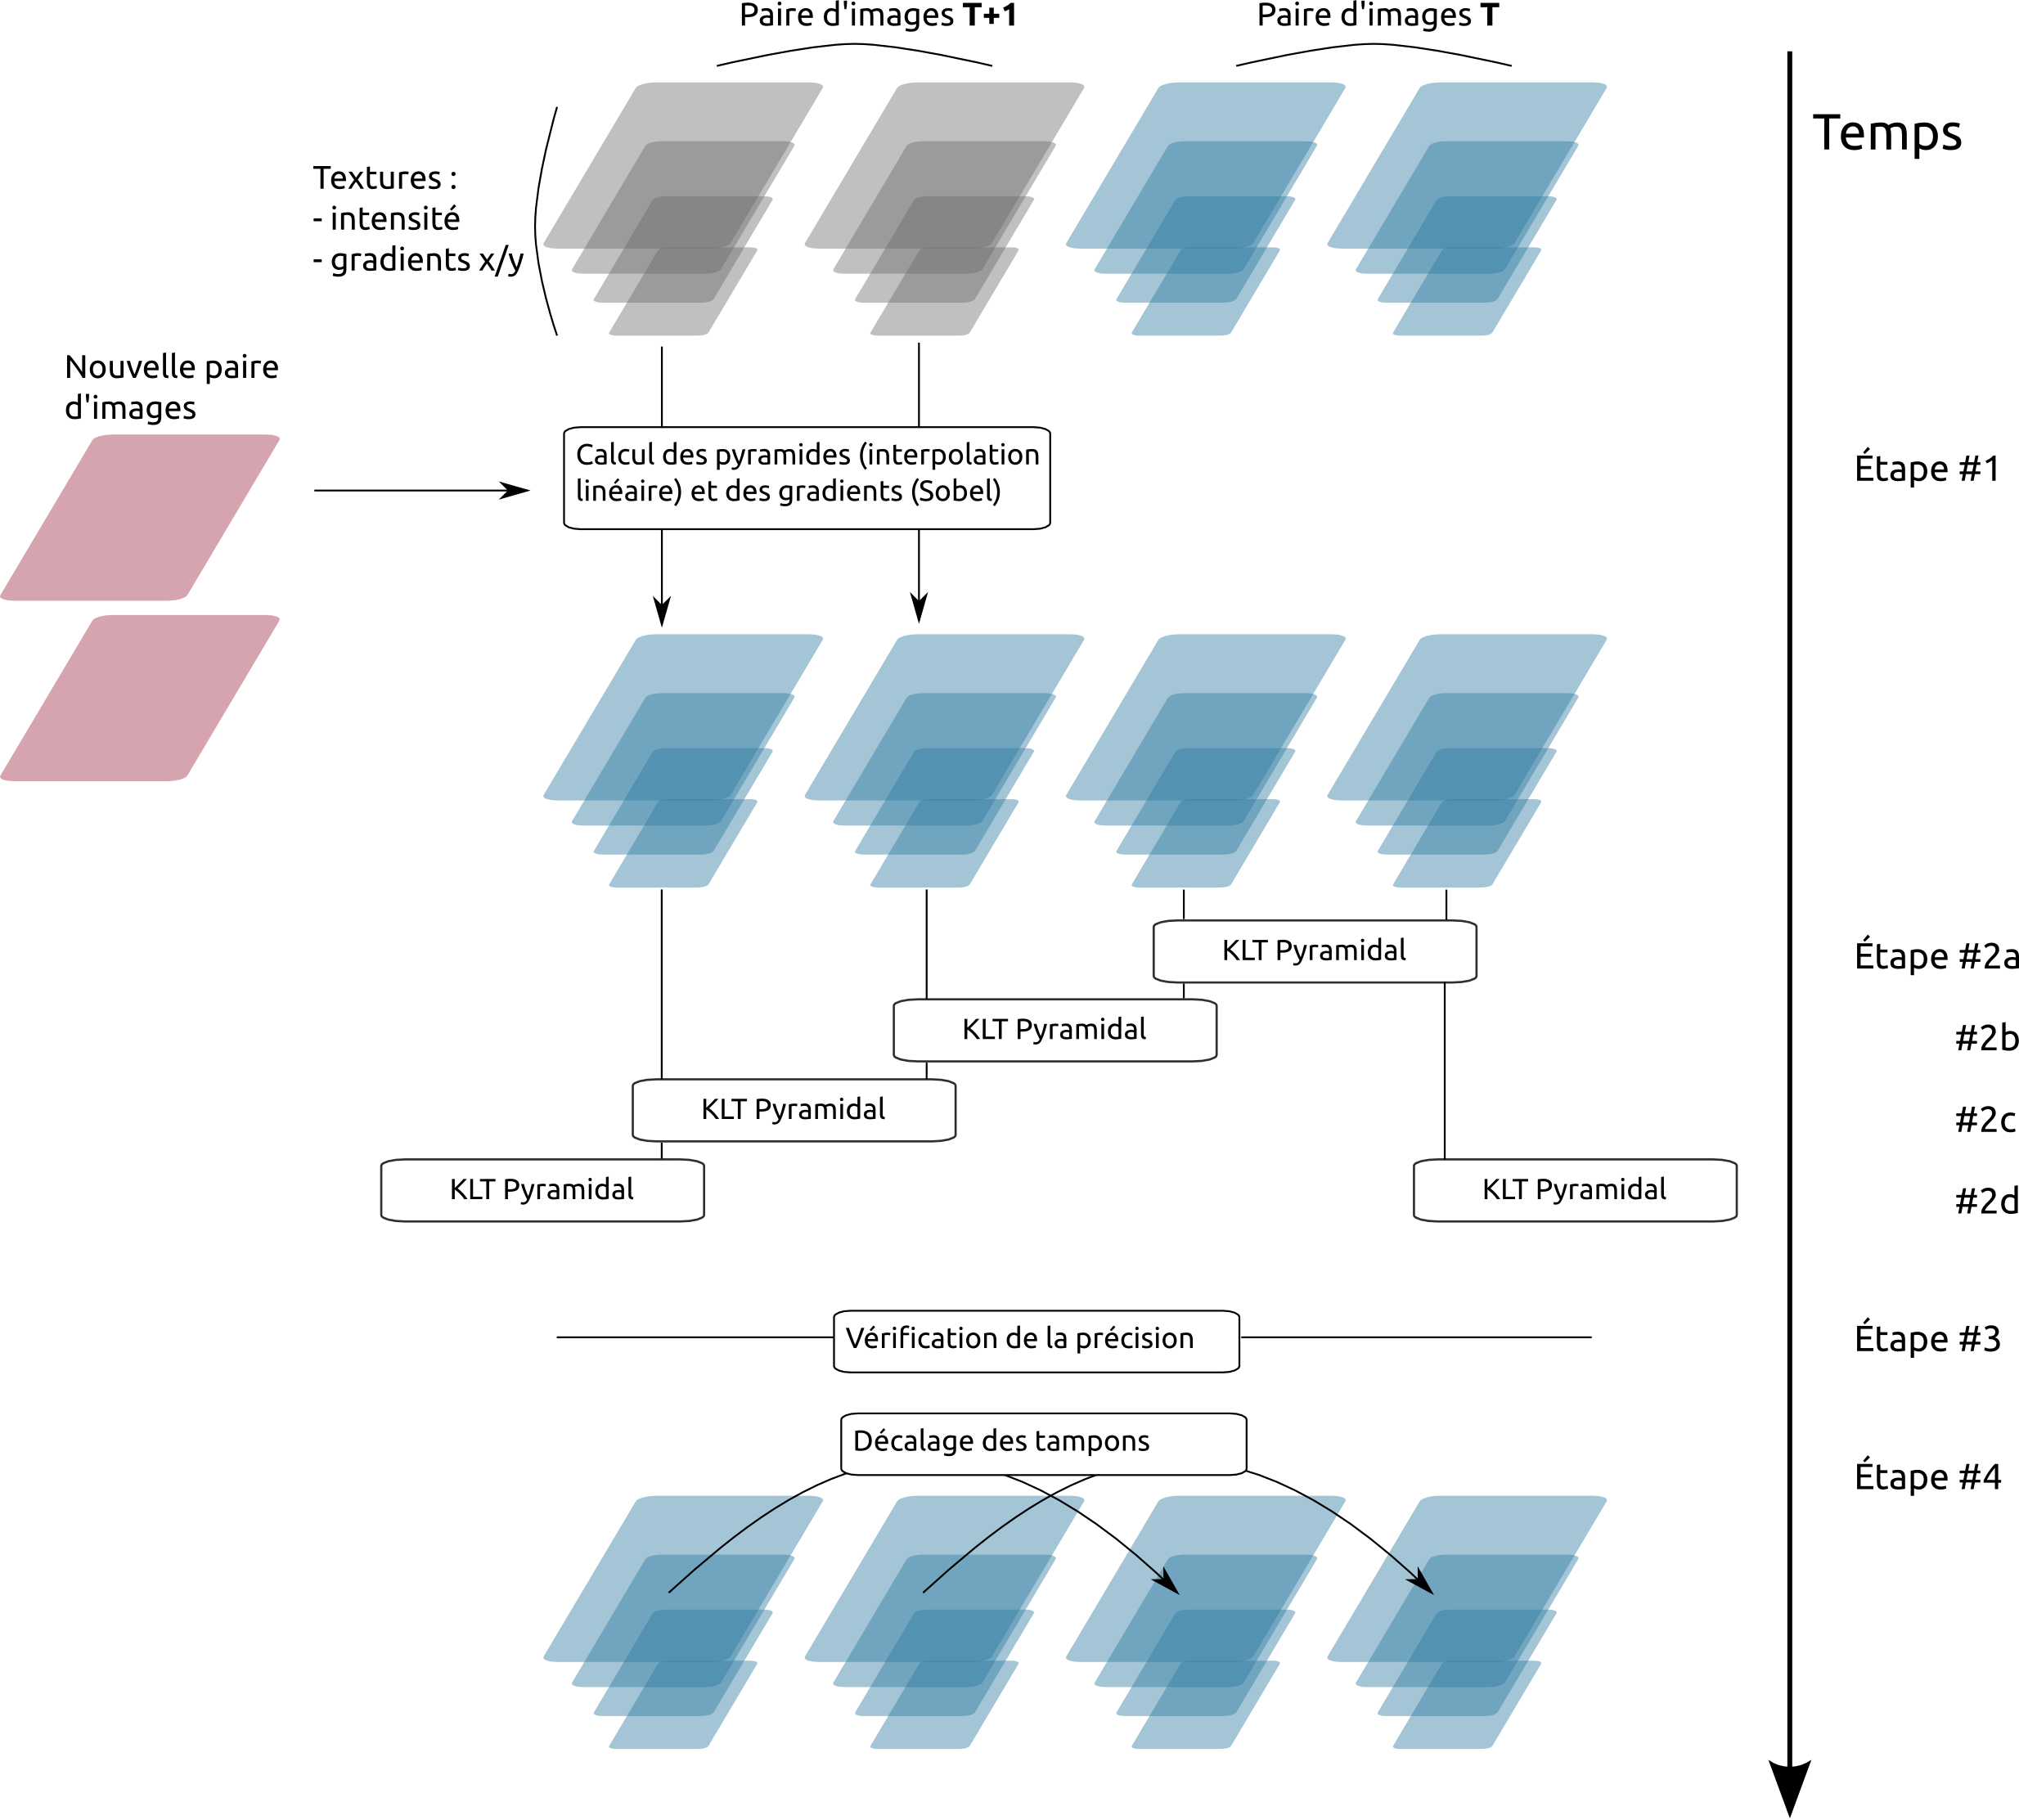
\includegraphics[width=1.3\textwidth]{Chapter3/graphics/4_Frames_implementation_diagram.png}
	}
	\caption{Vue d'ensemble de l'implémentation proposée pour un suivi redondant de points sur GPU. L'axe horizontal correspond à une exécution en parallèle, l'axe vertical correspond à une exécution séquentielle.}
	\label{fig:ch3_GPU_KLT}	
\end{figure}

\subsubsection{Comparaison : CPU/GPU}
Les performances en termes de robustesse et qualité du suivi sont équivalentes entre les différentes implémentations, comme attendu (s'agissant d'une application directe de \cite{Bouguet2001a} dans tous les cas). L'évaluation du temps de calcul est rendue délicate par sa dépendance à la plate-forme utilisée. On compare dans le tableau \ref{tab:ch3_comp_cpu_gpu} les performances obtenues par différents circuits présents dans le commerce, qui sont cependant en deçà de l'état de l'art en la matière (la GTX470 est sortie en 2010). Il s'agit donc de performances aisément accessibles en 2013, et un suivi de points plus ambitieux (quasi-dense) est sans doute possible. Le temps de calcul présenté vaut pour 4000 points, une taille d'image de 512 x 384, 5 étages de pyramide et un voisinage de 7x7 pixels. On note \emph{4Frame} notre implémentation purement CUDA conçue autour du suivi redondant sur 4 images. L'implémentation OpenCV-GPU présentée n'est pas spécialement optimisée pour notre tâche, il est sans doute possible de faire un peu mieux sans toutefois - à notre avis - atteindre les performances d'une implémentation dédiée. La version 2.4 de la librairie OpenCV est utilisée.

\begin{table}[H]
	\centerline {
		\begin{tabular}{| c | c | c | c | c | c |} 
			\hline
			Méthode & Support & Processeur & \pbox{5cm}{Unités \\ d'exécution} & \pbox{5cm}{Temps de \\ calcul (ms)} & Framerate\\
			\hline
			OpenCV & CPU & Intel Core i7 	& 4 	& 43 	& 23\\
			\hline
			OpenCV & GPU & nVidia GTX470	& 448 &	70 	& 14	\\
			\hline
			OpenCV & GPU & nVidia GTX460m & 192	& 115 & 9		\\
			\hline
			\textit{4Frame} & GPU & nVidia GTX470 	& 448 &\textbf{27} 	& \textbf{37}	\\
			\hline
			\textit{4Frame} & GPU & nVidia GTX460m & 192 & 42 	& 23	\\
			\hline
		\end{tabular}
	}
	\caption{Comparaison des temps de calculs selon différentes méthodes et unités de calcul. 4000 points sont suivis de manière redondante.}
	\label{tab:ch3_comp_cpu_gpu}
\end{table}

On pourra tout d'abord remarquer que le gain en performances attendu par une implémentation massivement parallèle (la GTX 470 dispose de 448 unités d'exécution, la GTX460m de 192 unités, contre 4 unités pour le CPU considéré) n'est pas directement observé en pratique. Les unités de calcul de type \og CPU\fg{} et \og GPU\fg{} ne sont tout d'abord par directement comparables, même si le nombre de processus exécutés simultanément est effectivement de l'ordre du nombre d'unités annoncées. Il est possible d'obtenir des performances significativement améliorées par l'implémentation très parallélisée, mais le caractère un peu aléatoire de la position des points à suivre est préjudiciable au cadre SIMD (\emph{Single Instruction Multiple Data} - Instruction Unique, Données Multiples) imposé par les GPU. Le facteur limitant du temps d'exécution d'un programme est par ailleurs beaucoup plus complexe que le seul nombre d'unités qui lui sont consacrées. \\

On pourra ensuite constater qu'une implémentation \og naïve\fg{} sur GPU n'est pas vraiment profitable dans cette application. Ceci peut s'expliquer par des transferts inutiles entre les espaces mémoire CPU/GPU, et par des tâches répétitives dans le cycle de suivi de point qui ne sont pas exploitées. On rejoint en cela une remarque précédente, signalant la grande disparité de performances possibles dans le cadre d'une implémentation massivement parallèle. On peut enfin remarquer que le gain obtenu entre les circuits \emph{470} et \emph{460m} est de l'ordre de 1.55, tandis que les unités d'exécution sont 2.3 fois plus importantes, ce qui laisse supposer que notre implémentation pourrait être améliorée.

\section{Conclusion}
On a présenté dans cette partie différentes méthodes de l'état de l'art pour extraire des informations à partir de flux d'images. Nous nous sommes concentrés sur le suivi de points singuliers dans une séquence d'images, bien que d'autres concepts puissent être mis en œuvre, et nous avons proposé un suivi de points redondant nous permettant d'évaluer en tout point la fiabilité du suivi. Une comparaison de différents algorithmes de détection de points d'intérêt nous a permis de sélectionner le détecteur de Shi et Tomasi comme étant le plus approprié pour notre application. Nous avons ensuite proposé une implémentation GPU du suivi redondant de points, et nous l'avons comparé à plusieurs implémentations de l'état de l'art. On peut finalement vérifier que le suivi fiable et en temps réel de plusieurs milliers de points est possible, ce qui nous amène à en proposer une exploitation dans le cadre de l'odométrie visuelle, de la reconstruction de l'environnement et de la détection d'objets mobiles.

\chapter{Odométrie visuelle, reconstruction 3D} 
\label{sec:ch4}
\vspace{10pt}

\minitoc
\clearpage

% % % % % % % % % % % % % % % % % % % % % % % % % % % % % % % % % % %
% Odométrie visuelle et reconstruction de l'environnement statique  %
% % % % % % % % % % % % % % % % % % % % % % % % % % % % % % % % % % %

\section{Introduction}
% On fait le constat que les informations obtenues précédemment ne sont pas suffisantes
Suite à l'étape précédente de perception visuelle par un dispositif de stéréo-vision, on dispose à cet étape d'un ensemble de points repérés dans le plan image et suivis dans le temps. On peut également le représenter comme une séquence de nuages de points positionnés en trois dimensions, et dont les associations temporelles individuelles sont connues. Ces informations ne sont pas de nature à répondre à certains de nos besoins, identifiés dans la section \ref{sec:ch1_besoins}, par exemple le positionnement du porteur dans son environnement ou la détection de l'espace navigable. Elles ne sont, par ailleurs, pas de qualité suffisante pour répondre précisément à d'autres tâches qui nous sont imputées, par exemple la détection des obstacles statiques, du fait d'un bruit de mesure très important.\\
% Conséquence : intégrer ces informations dans le temps -> on a besoin de déterminer l'ego-motion et de proposer un cadre pour la fusion des observations
Il est alors naturel de s'intéresser à l'intégration temporelle de ces mesures, afin d'améliorer leur précision par l'accumulation des observations, et d'obtenir les informations qui nous font défaut. Deux besoins sont immédiatement perceptibles : le mouvement du porteur doit être déterminé, afin de rendre ces observations cohérentes ; et une fusion de ces observations permettant d'obtenir des valeurs estimées doit être proposée. Ces deux problématiques sont intrinsèquement liées\footnote{Une erreur sur l'estimation du mouvement a en effet une incidence directe sur la qualité de l'accumulation des observations, tandis que ces observations sont elles-mêmes à la source de cette estimation.}, ce que leur estimation prend souvent en compte. On notera dans la suite \emph{ego-motion} le mouvement propre du porteur, comme il  est l'usage dans la littérature.\\
% Rapport au SLAM et résolution disjointe mouvement/position des points
Plusieurs méthodes présentes dans l'état de l'art proposent une résolution simultanée de ces deux problématiques, comme nous l'avons évoqué dans la section \ref{sec:ch2_Algo_total}, ce qui semble naturel du fait de leurs interactions. Cette approche est cependant intrinsèquement limitée dans le nombre de points qui peut alors être positionné, du fait de l'augmentation très rapide des dimensions du problème. Nous avons fait le choix d'une résolution disjointe, afin de pouvoir augmenter très nettement la densité de points traités par rapport à ces techniques, tout en conservant un temps de calcul raisonnable.\\
% Présentation du plan
On présentera quelques uns de ces enjeux dans une première partie, avec une revue de l'état de l'art dans les domaines de l'odométrie visuelle, et de la construction de nuages de points à partir d'observations multiples. On détaillera également quelques techniques parmi les plus utilisées en matière de filtrage et d'estimation robuste, ces techniques étant exploitées dans notre proposition. Une seconde partie nous permettra de présenter l'algorithme que nous proposons, pour estimer l'\emph{ego-motion} et la position des points observés, dont le fonctionnement général est décrit sur la figure \ref{fig:ch4_schéma_global}. Une troisième et dernière partie nous permettra d'aborder l'implémentation de notre proposition, ainsi que son évaluation sur des critères de précision ou de temps de calcul.

\begin{figure}
	\centering
	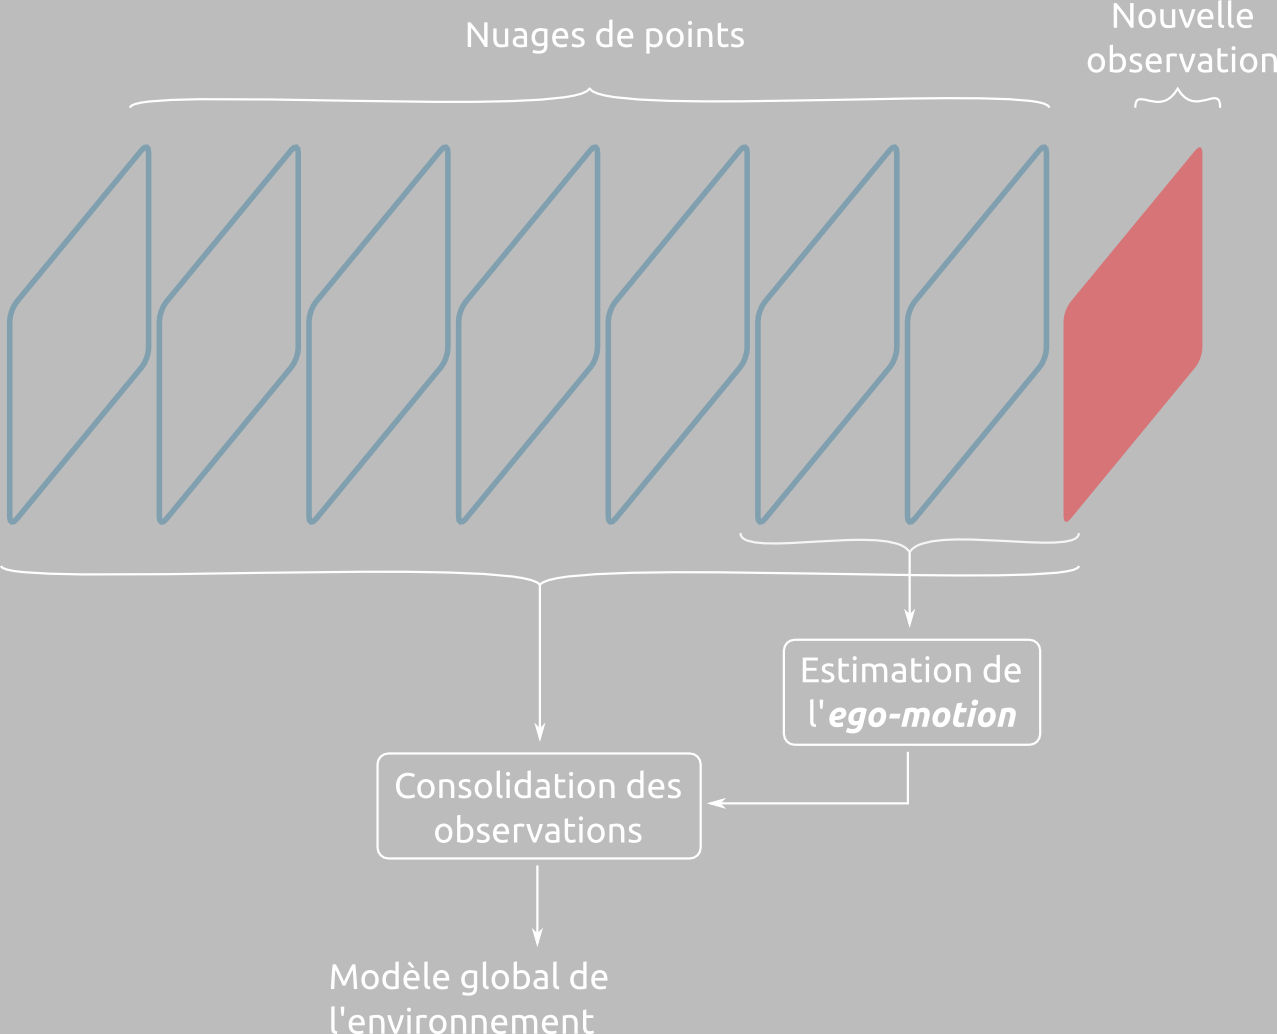
\includegraphics[width=0.8\textwidth]{Chapter4/graphics/overall_scheme.png}
	\caption{Représentation schématique du procédé proposé pour consolider les observations dans le temps et dans le référentiel du porteur. Les observations précédentes sont supposées  être dans un référentiel cohérent, la nouvelle observation étant associée à un nouveau référentiel.}
	\label{fig:ch4_schéma_global}
\end{figure}

\section{État de l'art} \label{sec:ch4_state_of_art}
On présente dans ce qui suit un état de l'art des méthodes répondant à tout ou partie de nos besoins. Il s'agit ainsi de recenser les techniques les plus efficaces en matière d'odométrie visuelle et de reconstruction de l'environnement à partir d'observations multiples, tout en conservant nos prérequis initiaux d'une exécution en temps réel et sur un grand nombre de points. On présente également quelques éléments de compréhension dans des domaines spécifiques, celui des estimateurs robustes et du filtrage, ces domaines étant mis à contribution dans l'approche  que nous proposons pour déterminer le mouvement du porteur.

\subsection{Odométrie visuelle} \label{sec:ch4_state_of_art_VO}
On distingue dans la suite les méthodes se situant dans l'espace image et les méthodes considérant l'espace en trois dimensions pour estimer l'ego-motion. Ces techniques peuvent être plus précisément classées selon l'espace dans lequel est reportée l'erreur d'estimation, c'est à dire l'erreur que l'on cherche à minimiser pour estimer le mouvement du porteur entre deux acquisitions. Ceci n'exclue pas nécessairement que l'une ou l'autre des représentations soit mise à contribution en tant qu'intermédiaire de calcul. On considère par ailleurs l'ensemble des techniques d'odométrie visuelle, qu'elles soient basées sur une configuration de type mono-vision ou stéréo-vision. \\
Il est souvent préférable de se situer pour cette estimation dans l'espace du capteur, c'est à dire dans le plan image dans notre cas. Changer de système de coordonnées (par exemple pour repasser dans l'espace en trois dimensions) peut en effet impliquer de faire intervenir des fonctions non-linéaires complexes, qui modifient notamment la forme de l'incertitude sur la mesure. Les traitements ultérieurs envisagés dans un système global de perception, en amont ou en aval de cette étape d'odométrie visuelle, peuvent cependant rendre une estimation dans l'espace 3D pertinente.
% Revenir sur la nécessité d'un suivi dans le temps -> suivi de point, de structure, d'une autre caractéristique (foyer d'expansion ?)

\subsubsection{Méthodes mono-caméra}
\paragraph{Approches classiques:\\}
% Première méthodes basées sur le déplacement d'éléments particuliers
L'estimation du mouvement à partir d'une séquence d'images est un problème ancien mais toujours étudié, et de nombreuses propositions sont présentes dans la littérature pour tenter d'y répondre. Notre synthèse de ce domaine ne sera sans doute pas exhaustive, mais on tentera d'en présenter les principales caractéristiques, ainsi que leur évolution historique. Les premières méthodes proposées se concentrent sur l'évolution de primitives dans l'image (lignes ou points dont l'identification est aisée), du fait des contraintes en termes de puissance de calcul alors prédominantes. L'utilisation de points plus flexibles (points saillants quelconques), ou du flux optique dans son intégralité est ensuite rapidement proposée. Plusieurs méthodes très diversifiées sont ainsi présentées par Tian \textit{et al} dans (\cite{Tian1996}).\\

La position du foyer d'expansion (point de convergence du flux optique) sert initialement de critère pour la détermination du mouvement rigide de translation entre deux images. Dans le cas d'un mouvement complet (translation et rotation), ces techniques déterminent tout d'abord le foyer d'expansion et la translation, avant de rechercher la composante de rotation du mouvement par minimisation du résidu entre flux optique calculé et observé. Ces considérations sont par ailleurs valables sur une surface planaire, le flux optique devant donc être initialement décomposé. La résistance au bruit de ces techniques repose enfin souvent sur un système de vote (\cite{Adiv1985}), qui privilégie le mouvement faisant consensus au détriment d'erreurs probables si de nombreux objets en mouvement sont observés. Cette dernière approche est toujours utilisée dans une technique plus récente basée sur les tenseurs d'orientation, pour le calcul du flux optique uniquement, la segmentation étant alors établie par croissance de région (\cite{Farneback2000}).\\

\paragraph{Approches globales:\\}
Des méthodes ont par ailleurs un statut particulier dans le domaine de l'odométrie visuelle, car elles résolvent ce problème conjointement avec la construction d'une carte de l'environnement. Il s'agit des approches de type SLAM, qui ont déjà été abordées dans la section \ref{sec:ch2_Algo_total} dans leur variante prenant en compte les objets mobiles de la scène. Deux approches principales sont présentes dans la littérature pour procéder à un SLAM, chacune disposant de points forts spécifiques : par optimisation, ou par filtrage.\\
Une approche par optimisation fonctionne, en général, en recherchant de manière itérative le déplacement minimisant une erreur de re-projection dans le plan image, à partir de points suivis dans le temps. Il s'agit par exemple du procédé proposé par Klein et Murray (\cite{Klein2007}, ou Zou dans une approche combinant si besoin plusieurs caméras (\cite{Zou}). Nister  (\cite{Nister2006}) propose cependant une méthode exploitant une optimisation robuste dans l'espace en trois dimensions. Les techniques suivies pour l'optimisation sont très différentes selon les propositions, une revue succincte pouvant notamment être lue dans \cite{Madsen2004}.\\

Plutôt qu'une estimation par optimisation, une approche par filtrage, souvent basée sur un filtre de Kalman étendu (EKF, \emph{Extended Kalman Filter}), est également possible. Les éléments du filtre sont alors des points singuliers de l'image, dont la position est initialement inconnue. Cette méthode permet notamment la prise en compte élégante d'un modèle de mouvement, qu'il est délicat d'inclure dans les méthodes par optimisation. Le filtrage autorise par ailleurs naturellement la prise en compte de l'historique des observations, dans l'hypothèse où le système est une chaîne de Markov de rang 1. Le nombre de points exploité pour l'estimation du mouvement est en revanche limité par les enjeux du traitement en temps réel. Le filtre de Kalman et ses dérivés nécessitent en effet l'inversion d'une matrice dont la taille est liée au nombres d'éléments du vecteur d'état, lequel croît avec le nombre de points pris en compte (cf. section \ref{sec:ch4_filtrage}). Cette inversion a un coût calculatoire de l'ordre de $O(d^{2.4})$ pour une matrice de dimension $d$, ce qui limite en pratique le nombre de points positionnés à quelques centaines d'unités. Cette méthode a été initialement proposée par Davison (\cite{Davison2003}), et a grandement été perfectionnée par la suite, notamment au niveau de l'initialisation de la covariance des points positionnés (\cite{Eade, Montiel, Ortega2007, Feraud2011}). La sélection des points utilisés doit alors faire l'objet d'une procédure robuste, par exemple grâce à un RANSAC (\emph{Random Sample Consensus}, Consensus à partir d'échantillons aléatoires, Fischler et Bolles \cite{Fischler1981}), pour éviter les erreurs liées au suivi de points mobiles. L'espace dans lequel se situe l'estimation du filtre dépend du modèle de mesure utilisé, mais il s'agit le plus souvent dans la littérature de l'espace image.\\

\subsubsection{Méthodes multi-caméras}
% Positions relative des caméras connue, ou non ?
D'autres techniques que celles présentées précédemment sont rendues possibles par l'utilisation de caméras supplémentaires, dont la configuration est connue ou non. La présence de ces points de vue disjoints permet de limiter les configurations mettant en défaut l'estimation du mouvement, bien que certains cas pathologiques soient toujours possibles (par exemple visible sur la figure \ref{fig:ch4_egomotion_vision_problem}).

\paragraph{Configuration des caméras inconnue:\\}
Ce cas de figure n'est pas courant dans le domaine de la stéréo-vision, mais il peut présenter un intérêt industriel ou expérimental, de part l'usage de caméras non-calibrées. Si la configuration relative des caméras est fixe, il est possible d'exploiter une détermination autonome du mouvement sur chacune des caméras, et d'estimer alors les paramètres de calibration de par les termes croisés induits par l'observation simultanée des mêmes éléments de la scène. Marquez-Gomez et Devy (\cite{Devy}) proposent ainsi d'utiliser un EKF  réparti sur deux caméras (BiCamSLAM) à même de répondre à cette problématique. Tout en conservant le formalisme de l'EKF dans un contexte de SLAM visuel, Bresson \textit{et al.} (\cite{Bresson2012}) proposent un algorithme décentralisé à même de positionner plusieurs entités indépendantes disposant chacune d'une unique caméra. \\
Il est par ailleurs toujours possible de confier à une optimisation globale la résolution des inconnues du système, parmi lesquelles les positions relatives des caméras présentes. Ces positions relatives peuvent alors varier dans le temps, au prix d'un coût calculatoire et d'une perte de précision importantes. Un positionnement collaboratif est alors possible, à partir de caméras individuelles \cite{Zou}, ou de paires de caméras calibrées \cite{Gil2010}.

\paragraph{Configuration des caméras connue au préalable:\\}
% - soit on minimise en 3D, soit on minimise l'erreur dans l'espace du capteur
La connaissance du changement de repère entre les plans image des différentes caméras permet d'obtenir une estimation directe de la position dans l'espace de points visibles simultanément sur chacun de ces plans. Deux approches sont alors possibles pour obtenir une estimation du mouvement, qui peuvent être dissociées par l'espace dans lequel l'erreur résiduelle se situe.\\
\begin{itemize}
	\item{} Dans le premier cas, il s'agit de minimiser par une technique robuste l'erreur dans l'espace en trois dimensions entre plusieurs observations de mêmes éléments, en déterminant ainsi la transformation rigide optimale. Ceci peut être réalisé selon des méthodes d'algèbre linéaire, comme c'est le cas avec d'autres capteurs (on peut ainsi se rapprocher de l'ICP (\emph{Iterative Closest Point}, itérations selon le point le plus proche), algorithme notamment utilisé pour le recalage de nuages de points obtenus par un télémètre laser, qui résout le problème de l'association des points dans le temps par une estimation itérative associant les points les plus proches, voir par exemple \cite{Rusinkiewicz}). Ces méthodes ont fait l'objet de nombreuses publications, et s'inscrivent plus généralement dans l'optimisation par moindres carrés (on pourra notamment voir \cite{Arun1987,Umeyama1991, Goryn1995, Eggert1997}). Une des méthodes de résolution, qui sera présentée dans la section \ref{sec:ch4_svd_pondérée}, exploite l'algèbre linéaire et la décomposition en éléments propres (SVD, \emph{Singular Value Decomposition}) d'une matrice de corrélation. Situant toujours l'erreur que l'on cherche à minimiser dans l'espace en trois dimensions, d'autres techniques permettent de prendre en compte plusieurs acquisitions consécutives dans une optimisation globale. Ces méthodes sont connues sous le nom de "Bundle Adjustment" (Ajustement de rayons), et de nombreux algorithmes sont utilisés dans ce cadre (\cite{Triggs2000}). Leur usage n'était historiquement pas temps réel, mais les progrès conjoints des algorithmes d'optimisation et des processeurs en font maintenant des solutions sérieuses pour l'estimation du mouvement (\cite{Niko2006, Konolige2008}). Une autre technique d'optimisation sur plusieurs observations consécutives est par ailleurs proposée par Lategahn et al. (\cite{Lategahna}), sans cependant prendre en compte (contrairement aux procédures de \emph{Bundle Adjustment}) la position des points observés dans l'espace. \\
	
	\item{} Ces méthodes situant l'optimisation dans l'espace cartésien en 3 dimensions décrivant le repère \og monde\fg{} ne sont en général pas optimales, dans le cas de l'utilisation d'un dispositif de stéréo-vision, comme nous l'avons notamment noté dans \ref{sec:ch2_Modèle Stéréovision} (une étude des conséquences de ce bruit anisotrope est notamment présente dans \cite{Blostein1987} et \cite{Sibley2007}, ce dernier considérant de plus les problèmes de biais liés à une mauvaise calibration). Il est donc souvent intéressant de minimiser une erreur dans le plan image. Celle-ci peut être dérivée explicitement à partir des équations de la stéréo-vision, tout en gardant un caractère linéaire (\cite{Demirdjian2001,Bak2011}). Cette optimisation peut également passer par une résolution non-linéaire à base de descente de gradient (méthodes de Levenberg-Marquardt ou Newton-Raphson), comme proposé dans de nombreuses publications ( \cite{Nister2006, Comport2010, Mei, Comport2010, Zou}). Dans une approche un peu différente, Agrawal\textit{ et al.} (\cite{Agrawal2007}) proposent d'associer l'estimation du mouvement à une fonction de coût robuste basée sur un algorithme de type RANSAC, dans le plan image. Le calcul des hypothèses de mouvement est linéaire et dans l'espace en trois dimensions, à partir des correspondances sélectionnées aléatoirement. Le score qui leur est associé est établi dans l'espace image et l'optimisation est dans ce cas non-linéaire (RANSAC).\\
\end{itemize}

\paragraph{Remarques sur une résolution linéaire adaptée à la stéréovision:\\} \label{ch4:méthode_bak}
Il est possible d'utiliser une méthode matricielle tout en prenant en compte les particularités du bruit de stéréo-vision. Une approche proposée par Bak (\cite{Bak2011}) autorise en effet une résolution élégante de cette problématique. A partir de l'expression des coordonnées des points dans le repère image d'un dispositif de deux caméras (en considérant donc les variables de position sur l'un des plans image, ainsi que la disparité), Bak en dérive l'effet d'une transformation rigide dans l'espace. Il réécrit alors l'équation \ref{eq:ch4_eq_to_minimize} dans le plan image, et obtient une équation linéaire pour laquelle beaucoup d'outils de résolution sont disponibles. Une méthode d'optimisation non-linéaire à base de RANSAC est par ailleurs utilisée pour rendre cette estimation plus robuste. \\
En reprenant les notations de Bak, les coordonnées des points dans l'espace image étendu s'écrivent :

\begin{equation}
	m_i = \left(  
		\begin{array}{c} 
			{x_m}_i		 \\ 
			 {y_m}_i	 \\ 
			{\delta_m}_i
		\end{array}
		\right) 
\end{equation}

Le problème à résoudre, reliant une transformation rigide $(R, T)$ dans l'espace 3D aux coordonnées projetées dans le système de stéréo-vision, s'écrit alors (avec $f$ la focale optique et $b_s$ la distance entre les deux caméras) :

\begin{align}
	\begin{split}
		&\left(
			\begin{array}{cccccc}
				-\frac{{x_m'}_1 \cdot {y_m}_1}{f} 		& -\frac{{x_m}_1 \cdot {x_m'}_1}{f} +f 	& -{y_m}_1 	& \frac{{\delta_m}_1}{b_s} & 0 & \frac{{\delta_m}_1 \cdot {x_m'}_1}{b_s}\\ 
				f -\frac{{y_m}_1 \cdot {y_m'}_1}{f} 	& \frac{{x_m}_1 \cdot {y_m'}_1}{f} 		& -{x_m}_1 	& 0 & \frac{{\delta_m}_1}{b_s} & \frac{{\delta_m}_1 \cdot {y_m'}_1}{b_s}\\ 
				\frac{{\delta'_m}_1 \cdot {y_m}_1}{f} 	& -\frac{{\delta_m'}_1 \cdot {x_m}_1}{f} & 0 & 0 & 0 & \frac{{\delta_m}_1 \cdot {\delta_m'}_1}{b_s}\\ 
				\cdots 									& \cdots 								& \cdots 	& \cdots 	& \cdots 	& \cdots\\ 
				-\frac{{x_m'}_N \cdot {y_m}_N}{f} 		& -\frac{{x_m}_N \cdot {x_m'}_N}{f} +f 	& -{y_m}_N 	& \frac{{\delta_m}_N}{b_s} & 0 & \frac{{\delta_m}_N \cdot {x_m'}_N}{b_s}\\ 
				f -\frac{{y_m}_N \cdot {y_m'}_N}{f} 	& \frac{{x_m}_N \cdot {y_m'}_N}{f} 		& -{x_m}_N 	& 0 & \frac{{\delta_m}_N}{b_s} & \frac{{\delta_m}_N \cdot {y_m'}_N}{b_s}\\ 
				\frac{{\delta'_m}_N \cdot {y_m}_N}{f} 	& -\frac{{\delta_m'}_N \cdot {x_m}_N}{f} & 0 & 0 & 0 & \frac{{\delta_m}_N \cdot {\delta_m'}_N}{b_s}
			\end{array} 
		\right) 
		\cdot  \lvert {
		\begin{array}{c}
			R\\ 
	 		T
		\end{array}
		} \\
		& \hspace*{5cm} = \left( {
		\begin{array}{c}
			{x_m}_1-{x_m'}_1			\\
			{y_m}_1-{y_m'}_1			\\
			{\delta_m}_1-{\delta_m'}_1	\\
			\cdots 						\\
			{x_m}_N-{x_m'}_N			\\
			{y_m}_N-{y_m'}_N			\\
			{\delta_m}_N-{\delta_m'}_N
		\end{array} }
		\right)
	\end{split}
\end{align}

Cette méthode est sans doute plus optimale que celle que nous proposons (section \ref{sec:ch4_robust_estimation}), mais ne profite pas de l'une des caractéristiques de la méthode par décomposition en éléments propres, à savoir sa dépendance très faible au nombre de points pris en compte. Le système à résoudre dans le cas d'une approche dite \og SVD\fg{} est de taille 3x3, quel que soit le nuage de points, tandis que cette approche conduit à un système dont la complexité est de l'ordre de $O(N^2)$. Les temps de calcul attendus sont donc relativement importants, ce que nous souhaitons éviter, au prix d'une perte de précision probable.

\subsubsection{Exploitation de capteurs tiers pour l'estimation de l'\textit{ego-motion}}
L'estimation de l'ego-motion à partir des informations visuelles peut ne pas être suffisante pour satisfaire tous les prérequis d'une navigation autonome. La vision peut ainsi être intrinsèquement mise en défaut (illumination problématique, vibrations, etc), tandis que la scène elle-même peut rendre l'odométrie impossible, sans que l'acquisition visuelle soit en faute (mouvement d'un élément tiers emplissant le champ visuel, voir la figure \ref{fig:ch4_egomotion_vision_problem} par exemple). Loin d'être des cas particuliers, ces phénomènes peuvent être couramment rencontrés dans des situations visées par un véhicule autonome au sein d'un cadre de vie propre aux humains, par exemple au sein d'une foule. \\

\begin{figure}
	\centering
	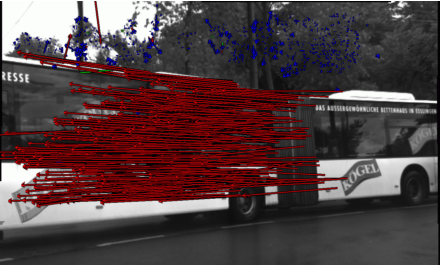
\includegraphics{Chapter4/graphics/problematic_scene.png}
	\caption{Exemple de situation problématique pour l'estimation purement visuelle de l'ego-motion. Les éléments statiques de la scène sont très minoritaires, du fait du masquage produit par un objet mobile. Illustration tirée de l'article \cite{Badino2008}}	
	\label{fig:ch4_egomotion_vision_problem}
\end{figure}

Il est donc assez naturel de chercher à corriger ce problème par la fusion d'informations de plusieurs capteurs complémentaires, comme un odomètre, un outil de positionnement satellitaire global (dit \emph{GNSS, Global Navigation Satellite System} dans la littérature anglo-saxonne, tel que le GPS, GLONASS ou Galiléo), ou encore un capteur de mouvent type IMU. L'utilisation d'un filtre de type EKF ou UKF fournit un cadre élégant pour la fusion de données, les différents capteurs étant associés à un modèle permettant la comparaison de leurs apports sur une base commune. Ce dispositif est particulièrement adapté au traitement temps réel, de part son caractère itératif, et la relative constance du temps de mise à jour. Leur couplage avec un algorithme de détermination de l’\emph{ego-motion} par indices visuels est présent dans la littérature (par exemple \cite{Singh2005,Bak2011}), mais l'utilisation d'autres capteurs est également possible, notamment les télémètres lasers (\cite{Weyers2011}). Une prise en compte par optimisation étant également possible (voir par exemple \cite{Martinelli2012}), même si sa mise en œuvre en temps réel est plus complexe.

\subsection{Génération de l'environnement à partir d'observations successives}
\paragraph{Approches récursives:\\}
La construction d'un nuage de points représentatif de la scène rentre explicitement dans les pré-requis du SLAM, on citera donc ici quelques exemples remarquables de la littérature à ce sujet. Ce sujet a déjà été abordé au point \ref{sec:ch4_state_of_art_VO}, et on pourra donc rapidement aborder la proposition initiale de Davison basée sur un filtre EKF (\cite{Davison2003}), et quelque unes des nombreuses évolutions ont été proposées. Montiel \textit{et al.} (\cite{Montiel}) ont ainsi proposé une paramétrisation améliorée de l'incertitude sur la position des amers visuels lors de leur introduction dans le filtre, afin de mieux gérer la non-linéarité dans l'estimation de la position liée à la distance au capteur (\emph{Inverse Depth Parametrization}). La covariance sur la position de l'amer est liée à l'inverse de sa distance au centre optique, cette paramétrisation étant modifiée pour revenir à une estimation directe dès que l'amer est suffisamment bien localisé). Tout en conservant une estimation par un filtre, Eade et Drummond (\cite{Eade}) proposent un algorithme autorisant la perception d'une carte de dimension beaucoup plus importante : dans la proposition de Davison, le filtre conserve à tout moment les covariances de chacun des amers estimés dans une unique matrice, ce qui rend le processus de mise à jour de l'ordre de O($N^2$) avec $N$ le nombre de points\footnote{Ce coût optimal était jusqu'à 2010 de très exactement $N^{2.376}$ pour l'algorithme de Coppersmith-Winograd (\cite{Coppersmith1990}). Stothers (\cite{Stothers2010}) en proposa alors une amélioration ramenant ce coût à $N^{2.374}$. Ce chiffre a été très légèrement amélioré depuis.}. Eade propose d'utiliser un filtre particulaire (se basant en cela sur les travaux de FastSLAM \cite{Thrun2004a}) à même de gérer le problème de l'association des observations, tandis que les covariances des points estimés sont dissociées. Pollefeys \textit{et al.} montrent par ailleurs (\cite{Pollefeys2007}) qu'il est possible de reconstruire un environnement très dense en accumulant les informations de cartes de profondeur, recalées par une estimation indépendante du mouvement. Les points positionnés ne sont dans ce cas pas suivis dans le temps, mais l'environnement statique convient très bien à cette approche. De même, Lategahn \textit{et al.} (\cite{Lategahn2011}) propose une approche relativement similaire, à ceci près que la disparité est dans ce cas filtrée dans le temps par un filtre de Kalman (individuel, au niveau de chaque pixel).\\

\paragraph{Approches par optimisation:\\}
L'estimation peut également se baser sur une optimisation (qui peut alors prendre en compte plusieurs observations consécutives) pour estimer la position des points observés. Mouragnon (\cite{Mouragnon2006}) propose le premier cette approche, suivi de Klein et Murray qui proposèrent un algorithme connu sous le nom de PTAM (\cite{Klein2007}), dissociant dans ce cas l'estimation de l’ego-motion et l'estimation de la position des points en deux processus différents. De même, Strasdat \textit{et al.} (\cite{Strasdat}) montrent que l'optimisation sur plusieurs acquisitions est nécessairement plus performante en termes de précision par rapport à une approche par filtrage (au prix d'une possible perte de généralité), et proposent un algorithme combinant une estimation initiale des positions des amers par filtrage (compatible avec l'usage de mono-vision), complétée par une optimisation postérieure. Dans le cas d'un dispositif de stéréovision, l'estimation de la position des amers peut assez naturellement faire l'objet d'un processus par optimisation, comme proposé par Konolige et Agrawal (\cite{Konolige2008}). On pourra remarquer que cette problématique d'estimation de la structure de l'environnement à partir d'images n'est pas nouvelle, et est présente sous le nom de photogrammétrie dans la littérature. Son utilisation en temps réel et dans le cadre de la robotique est plus récente, mais de nombreuses études sont d'ores et déjà disponibles et exploitables dans le domaine du SLAM. On pourra citer à cet effet la très complète revue de Triggs \textit{et al.} (\cite{Triggs2000}).

\section{Filtrage}  \label{sec:ch4_filtrage}
On décrit ici quelques algorithmes parmi les plus utilisés pour répondre à des besoins de filtrage, c'est à dire d'estimation de variables à partir d'observations stochastiques. Cet état de l'art est ici nécessaire de part l'algorithme que nous proposons, qui en fait usage, bien que d'autres approches s'attachent à la problématique de l'odométrie visuelle sans y recourir. Le lecteur souhaitant une synthèse plus avancée de quelques uns des filtres présentés ci-dessous pourra notamment se référer à la revue \cite{Chen2003}. On ne rappelle pas dans la suite la formulation du filtre de Kalman, qui est présente en annexe de ce manuscrit (\ref{sec:Annexe_kalman}), mais on s'attachera à en présenter deux variantes qui permettent son utilisation dans notre domaine.

\subsection{Filtre de Kalman étendu}
\subsubsection{Introduction:}
Comme de nombreux filtres Bayésiens, cet algorithme fonctionne en deux étapes : l'état futur du filtre est prédit, puis comparé à la nouvelle mesure, ce qui permet finalement d'en estimer un état corrigé. Il se restreint cependant à des prédictions et mesures linéaires, du fait de sa formulation matricielle. Cette restriction est importante, car elle limite beaucoup son usage en pratique. De nombreuses applications intègrent en effet une composante non-linéaire, du fait d'un changement de repère par exemple (coordonnées polaires/cartésiennes), ou d'un modèle de capteur complexe. Il est heureusement possible d'étendre l'usage du filtre de Kalman en linéarisant localement les fonctions de propagation ou de mesure, selon les principes posés par le développement de Taylor de fonctions non-linéaire. L'algorithme est alors nommé filtre de Kalman étendu, ou encore \emph{EKF} (Extended Kalman Filter) dans la littérature. 

\subsubsection{Propagation:}
On approxime localement les fonctions de propagation et de mesure par la première composante de leur développement de Taylor, ce calcul étant à renouveler dès que le point de fonctionnement ou de mesure est modifié. Les calculs sont alors essentiellement les mêmes que pour le filtre de Kalman classique, si l'on excepte l'usage dans l'étape de prédiction de fonctions non-linéaires quelconques, et l'apparition des matrices Jacobiennes (matrice des dérivées partielles) modélisant la contribution linéarisable de ces fonctions dans le calcul du gain de Kalman et de la mise à jour de la covariance. On note $G$ la matrice jacobienne de la fonction de propagation $g$, et de même $H$ la matrice jacobienne de la fonction de mesure $h$. 
\begin{enumerate}
	\item{\textbf{Prédiction:}}
	\begin{align}
		\bar{\mu}_t    	&= g(u_t, \mu_{t-1}) \label{eq:EKF_pred1} \\ 
		\bar{\Sigma}_t 	&= G_t \Sigma_t G_t^T + R_t \label{eq:EKF_pred2}\\ \nonumber
	\end{align}
	
	\item{\textbf{Calcul du gain $K_t$:}}
	\begin{align}
		K_t	&= \bar{\Sigma}_t H_t^T \left( H_t \bar{\Sigma}_t  H_t^T  + Q_t\right)^{-1}	\label{eq:EKF_KG}\\	\nonumber
	\end{align}
	
	\item{\textbf{Mise à jour:}}
	\begin{align}
		\mu_t 			&= \bar{\mu}_t + K_t \left(z_t - h(\bar{\mu_t}) \right) \label{eq:EKF_up1}\\
		\Sigma_t		&= \left( I - K_t H_t \right) \bar{\Sigma}_t \label{eq:EKF_up2}
	\end{align}
\end{enumerate}
Ces équations sont bien sûr à rapprocher des équations du filtre de Kalman original (\ref{eq:KF_pred1} à \ref{eq:KF_up2}). L'estimation du premier moment ($\mu$) fait appel aux fonctions de propagation et de mesure sous leur forme \og native\fg{} (non-linéaire), tandis que l'estimation de la covariance $\Sigma$ fait appel à une forme linéarisée de ces mêmes fonctions. Ce procédé est très utilisé, du fait de bonnes performances et de son coût calculatoire qui reste mesuré (les matrices jacobiennes n'étant pas nécessairement calculées à chaque itération, ce coût peut se rapprocher de celui d'un filtre \og classique\fg{}). \\

\subsubsection{Remarques:}
Le filtre de Kalman étendu, s'il est sans doute le moyen le plus utilisé de nos jours pour estimer l'état de systèmes complexes, n'est théoriquement utilisable que dans les approximations du développement de Taylor. Ces dernières engendrent deux types de limitations restreignant l'efficacité de l'EKF : les fonctions développées ($g$ et $h$) doivent être linéarisables (les termes d'ordre supérieur à 1 de leur développement de Taylor sont localement négligeables), et la distribution de l'état estimé doit être restreinte par rapport à la zone de validité du développement de Taylor. Cette dernière limitation est certainement la moins évidente, mais elle doit être prise en compte notamment dans les estimations non-consistantes des EKF dans certains cas pathologiques (l'estimation de la covariance devient inférieure à la covariance réelle, la confiance accordée à l'état de sortie du filtre est surestimée).

\subsection{Filtre de Kalman inodore}
Proposé par Julier et Uhlmann (\cite{Julier1997}), le Filtre de Kalman Inodore (ou UKF - \emph{Unscented Kalman Filter}) adopte une approche différente pour prendre en compte les problématiques de linéarisation inhérentes à la formulation matricielle du filtre de Kalman. Ce filtre se base sur la transformation dite inodore, qui modélise une gaussienne par un nombre fini de particules $\chi$ (aussi appelés \emph{points sigma}). Une transformation réciproque est possible pour obtenir les deux premiers moments de la distribution à partir de ces particules, cette transformation étant exacte dans le cas d'une gaussienne. Elle est décrite dans \ref{eq:ch4_transformation_inodore}, la transformation inverse étant décrite dans \ref{eq:ch4_transformation_inodore_inverse}. 

\subsubsection{Transformation Inodore (\emph{UT}):}
Le nombre de dimensions de notre vecteur d'état est noté $n$, la transformation inodore génère donc $2n+1$ points. Les poids associés à ces particules (utilisés dans la transformation inodore inverse) sont différents pour le calcul de la moyenne et de la covariance, et sont respectivement notés $\omega_\mu$ et $\omega_\Sigma$.

\begin{enumerate}
	\item{\textbf{Calcul des points sigma:}}\\
	Avec $\left( \sqrt{(n+\lambda) \Sigma }\right)_i$ la colonne (ou ligne) $i$ de la matrice racine de $(n+\lambda) \Sigma$.
	\begin{align} \label{eq:ch4_transformation_inodore}
		\begin{split}
			\chi{[0]} &= \mu \\
			\forall i \in {1,..,n} \qquad \chi{[i]} &= \mu + \left( \sqrt{(n+\lambda) \Sigma }\right)_i \\
			\forall i \in {n+1,..,2n} \qquad  \chi{[i]} &= \mu - \left( \sqrt{(n+\lambda) \Sigma }\right)_i \\
		\end{split}
	\end{align}
	
	\item{\textbf{Calcul des poids correspondants:}}
	\begin{align}
		\begin{split}
			\omega_\mu^{[i]} &= \frac{\lambda}{n+\lambda} \\
			\omega_\Sigma^{[i]} &= \frac{\lambda}{n+\lambda} (1 - \alpha^2 +\beta)
		\end{split}
	\end{align}
\end{enumerate}

$\lambda$ est ici un paramètre d'échelle, qui vaut \emph{n-3} dans le cas d'une distribution Gaussienne. L'estimation n'est cependant pas limitée aux variables aléatoires distribuées selon la loi normale, la répartition des points sigma pouvant être choisie pour prendre en compte des distributions légèrement différentes. On peut alors modéliser le paramètre $\lambda$ par :
\begin{equation}
\lambda = \alpha^2(n + \kappa) -n % //REVENIR SUR LES DEFINITIONS DE ALPHA/BETA/GAMMA..
\end{equation}

avec $\alpha$, $\beta$ et $\kappa$ des paramètres de dispersion pouvant être arbitrairement choisis pour mieux estimer différentes distributions ($\beta = 2$  pour une distribution gaussienne). Cette adaptation à des distribution autres que gaussiennes est l'un des intérêts l'UKF, bien que l'EKF soit lui même relativement résistant à l'estimation de variables aléatoires dont la distribution diffère légèrement de la loi normale.\\

\subsubsection{Transformation Inodore inverse:}
La transformation inverse s'écrit comme un calcul de moyenne et de covariance pondérés par les points sigma propagés, notés ici $\mathcal{Y}^{[i]}$ :
\begin{align} \label{eq:ch4_transformation_inodore_inverse}
	\begin{split}
		\hat{\mu} &= \sum\limits_{i=0}^{2n} \omega_m^{[i]} \mathcal{Y}^{[i]} \\
		\hat{\Sigma} &= \sum\limits_{i=0}^{2n} \omega_c^{[i]} \left( \mathcal{Y}^{[i]} - \hat{\mu} \right) \left( \mathcal{Y}^{[i]} - \hat{\mu} \right)^T
	\end{split}
\end{align}

\subsubsection{Propagation:}
La propagation du filtre dans son intégralité s'écrit enfin :
\begin{enumerate}
	\item{\textbf{Prédiction:}}\\
	Des points sigma sont générés, décrivant l'état précédent du filtre, ils sont propagés par la fonction \emph{g} puis la distribution de l'état propagé est modélisée par les paramètres de moyenne et de covariance.
	\begin{align}
		\chi_{t-1}{[i]}, \omega_m^{[i]}, \omega_c^{[i]} &= UT(\mu_{t-1}, \Sigma_{t-1}) 			\label{eq:UKF_pred1}\\
		\chi_{t-1, t}{[i]}								&= \left\lbrace g(u_t, \chi_{t-1}{[i]})	\right\rbrace  	\label{eq:UKF_pred2}\\
		\left(\bar{\mu_t}, \bar{\Sigma_t} \right) 		&= UT^{-1}(\chi_{t-1, t}{[i]}, \omega_m^{[i]}, \omega_c^{[i]} ) + R_t \label{eq:UKF_pred3}\\	\nonumber
	\end{align}
	
	\item{\textbf{Mesure:}}\\
	Un nouvel ensemble de points sigma est généré à partir de l'état propagé, cet état est \og projeté\fg{} sur l'espace de mesure en utilisant la fonction \emph{h} (\ref{eq:UKF_meas2}), la mesure prédite (avec sa covariance) est capturée par \ref{eq:UKF_meas3}, tandis que la covariance liée à l'action de mesurer est capturée par $\bar{\Sigma}_t^{x,z}$ (\ref{eq:UKF_meas4}). 
	\begin{align}
		\hat{\xi_{t}{[i]}}, \omega_{m,z}^{[i]}, \omega_{c,z}^{[i]}	&= UT(\hat{\mu_t}, \hat{\Sigma_t})	\label{eq:UKF_meas1}\\
		\hat{\mathcal{Z}_{t}{[i]}}	&= h(\hat{ \xi_{t}{[i]} }) \label{eq:UKF_meas2}\\
		\left(\hat{z_t}, \bar{S_t} \right) &= UT^{-1}( \mathcal{Z}_{t}{[i]}, \omega_{m,z}^{[i]}, \omega_{c,z}^{[i]} ) + Q_t 		\label{eq:UKF_meas3}\\
		\bar{\Sigma}_t^{x,z} &= \sum\limits_{i=0}^{2n} \omega_c^{[i]} \left( \xi_{t}{[i]} - \bar{\mu_t} \right) \left( \mathcal{Z}_{t}{[i]} - \hat{z_t}\right)^T	\label{eq:UKF_meas4}\\	\nonumber
	\end{align}
	
	\item{\textbf{Calcul du gain:}}\\
	Le gain de Kalman est calculé en prenant en compte la covariance de la mesure prédite, et celle intrinsèque à la fonction de mesure $h$.
	\begin{align}
		K_t &= \bar{\Sigma}_t^{x,z} \bar{S_t}^{-1} 		\label{eq:UKF_prop1}\\ \nonumber
	\end{align}
	
	\item{\textbf{Mise à jour:}}\\
	Comme dans un filtre de Kalman classique, l'état corrigé est relatif à l'innovation $z_t - \hat{z_t}$ et au gain $K_t$ calculé préalablement.
	\begin{align}
		\mu_t &= \bar{\mu_t} + K_t(z_t - \hat{z_t}) 	\label{eq:UKF_prop2}\\
		\Sigma_t &= \bar{\Sigma_t} - K_t S_t K_t^T		\label{eq:UKF_prop3}\\ \nonumber
	\end{align}
\end{enumerate}

La gestion des transformations non-linéaires (propagation comme mesure) est immédiate, celles-ci étant appliquées sur les points sigma, avant d'utiliser la transformation inodore inverse. Contrairement à l'EKF, la linéarisation des transformations n'est donc ici pas nécessaire, pas plus que le calcul (parfois coûteux) de son jacobien. Dans le cas de fonctions linéarisables, et d'états estimés dont la covariance est restreinte par rapport à cette hypothèse de linéarisation, les performances respectives des filtres EKF et UKF sont identiques. L'augmentation de la covariance des états estimés, ou le besoin d'utiliser des fonctions fortement non-linéaires introduit cependant un avantage compétitif de l'UKF, comme très bien mis en avant dans l'article fondateur de Julier et Uhlmann (\cite{Julier1997}). Le coût calculatoire de l'extension inodore de l'UKF reste par ailleurs très modestes par rapport à un KF ou à un EKF, la gestion de particules supplémentaires étant en général très rapide devant les coûts liés au calcul matriciel de grande dimension.\\

Bien que la génération de particules les rapproche, l'UKF est bien différent d'un filtre dit \og à particules\fg{} (voir section \ref{sec:ch4_filtre_particule}). Il modélise tout d'abord, comme le KF et l'EKF, la distribution des variables par leur deux premiers moments statistiques ; ce qui le restreint à la prise en compte de distributions mono-modales et symétriques. La transformation entre l'état du filtre et les particules (\og points sigma\fg{} donc) est par ailleurs déterministe dans le cas de l'UKF, et nécessite peu de particules, tandis qu'un filtre particulaire se base sur un grand nombre de tirages aléatoires pour modéliser la distribution de la variable estimée.

\subsection{Filtre à particules} \label{sec:ch4_filtre_particule}
Ce filtre exploite une méthode introduite dans les années 1940, et dont le développement plus récent est notamment lié à l'accroissement de la puissance de calcul disponible (et à sa simplicité pour évaluer le résultat numérique de calculs non-résolubles analytiquement). Il s'agit de la méthode dite de \emph{Monte Carlo}, qui consiste à estimer, selon la loi des grands nombres, un calcul fonction d'une distribution de probabilité initiale par l'étude du résultat d'un grand nombre de tirages. Cette méthode ne souffre d'aucune des limitations couramment associées au filtres numériques (transformation quelconque, fonction de distribution potentiellement quelconque - si tant est que l'on sache produire un grand nombre d'échantillons selon cette distribution -), la précision obtenue étant cependant fonction du nombre de tirages et de l'adéquation entre la distribution initiale et celle que l'on souhaite observer.\\
Une explication précise de ce phénomène est notamment disponible dans le livre de S. Thrun (\cite{Thrun2005}). L'étude de cette problématique explique notamment le développement de la technique dite d'\emph{importance sampling}, et peut sommairement s'expliquer par la compression et la dilatation de la distribution initiale le long des non-linéarités de la fonction de propagation ou de mesure du filtre.

\subsection{Comparaison : estimation d'une variable aléatoire propagée par une fonction non-linéaire}
On illustre dans la Figure \ref{fig:ch4_transformation_evaluation} certains des mécanismes à l’œuvre dans les différentes implémentations des filtres de Kalman décrits précédemment. L'enjeu de ces différentes implémentations est le suivant : on dispose initialement d'une variable aléatoire dont la distribution est gaussienne, ce qui correspond à un cas pratique relativement courant. Cette variable est soumise à une transformation non-linéaire, qui peut correspondre à une fonction de propagation ou à une fonction de mesure, et il s'agit de prédire la distribution attendue. On illustre ici les conséquences des approximations à l’œuvre dans l'EKF (la transformation est linéarisée selon sa matrice jacobienne à la valeur moyenne de la distribution incidente), et dans l'UKF (des points sigma sont générés selon la distribution initiale, propagés selon la fonction non-linéaire connue, et une nouvelle distribution est déduite de ces points propagés). Les autres étapes du filtre (gain de Kalman et correction) sont par ailleurs très similaires entre ces différents algorithmes, ce qui souligne l'importance de cette étape de propagation de l'état d'une variable aléatoire.\\

\subsubsection{Cas pratique:}
Dans la Figure \ref{fig:ch4_transformation_evaluation}, on représente la distribution initiale de la variable aléatoire selon l'axe des abscisses. La transformation retenue est exponentielle (donc fortement non-linéaire), elle est représentée dans le même repère. On reporte les éléments transformés sur l'axe des ordonnées, de sorte que cette figure pourrait être construite à la main par simple report de valeurs relativement à la fonction de transformation. Autrement dit, l'espace initial est selon l'abscisse, l'espace final est selon l'ordonnée. Cette représentation est assez commune dans la littérature, étant par exemple reprise par Thrun dans \cite{Thrun2000}.\\
La distribution exacte de la variable aléatoire dans l'espace d'arrivée est obtenue par une simulation \og Monte-Carlo\fg{}, impliquant plusieurs millions de tirages. Elle représente la distribution propagée exacte. On représente les points sigma initiaux, projetés sur l'espace d'arrivée, ainsi que la gaussienne qui en est obtenue. On représente par ailleurs la distribution obtenue lorsqu'on linéarise la transformation, comme c'est le cas dans un filtre EKF. Les différentes valeurs moyennes (exacte, obtenues par transformée inodore et par linéarisation) sont par ailleurs représentées avec une notation similaire.

\begin{figure} 
	\centering
	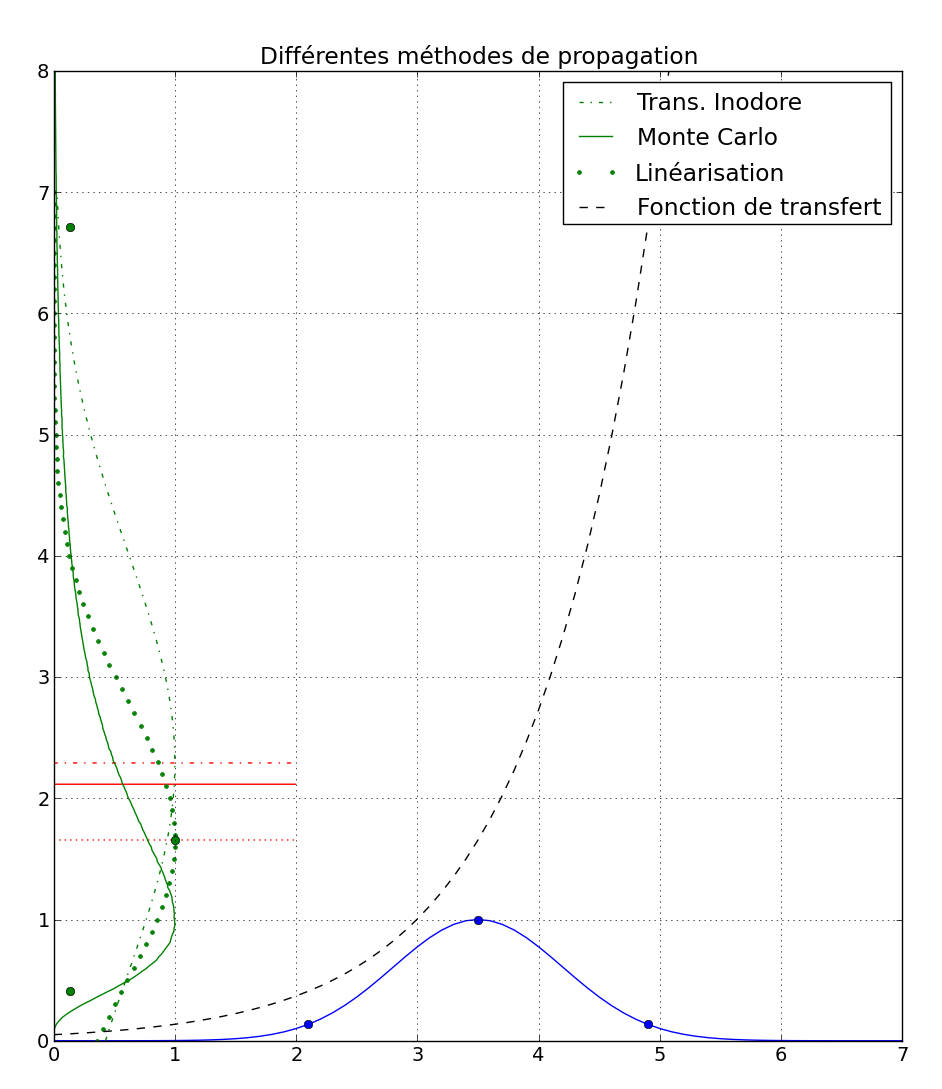
\includegraphics[width=0.7\textwidth]{Chapter4/graphics/unscented_transform.png}
	\caption{Illustration de différents procédés de propagation d'une variable aléatoire. La courbe bleue représente la distribution initiale. Les courbes vertes représentent les distributions propagées, de manière exacte (continue) ou approximatives. Les lignes rouges représentent les valeurs moyennes estimées de la variable propagée}
	\label{fig:ch4_transformation_evaluation}
\end{figure}

\subsubsection{Remarques:}
Plusieurs éléments sont à remarquer sur la Figure \ref{fig:ch4_transformation_evaluation}, très dense en informations. La transformation utilisée étant non-linéaire et non-symétrique par rapport à la valeur moyenne de la variable initiale, la distribution de la variable aléatoire dans l'espace d'arrivée est fortement dissymétrique, elle ne correspond pas à une gaussienne (son troisième moment statistique, le \og \emph{skew}\fg{}, n'est pas nul. Ce troisième moment est par construction nul pour une loi normale). On peut remarquer que l'usage de la transformée inodore permet de capturer une partie de cette dissymétrie (les points sigma ne sont pas non plus symétriques dans l'espace d'arrivée), mais l'estimation d'une gaussienne à partir de ces points perd cette information. La transformée inodore inverse consiste en effet à calculer les deux premiers moments modélisés par les points sigma. Dans cet exemple (les performances des différentes approches varient avec la transformation choisie, notre cas n'en est qu'une illustration), les paramètres estimés sont présentés dans le tableau \ref{tab:ch4_comparaisons_linéarisation}.

\subsubsection{Quelques résultats:}
On recense dans le tableau \ref{tab:ch4_comparaisons_linéarisation} les résultats des estimations des deux premiers moments statistiques de la variable propagée, selon les méthodes de linéarisation et de transformation inodore. On pourra retenir que la linéarisation est efficace si la variance de l'état d'entrée est faible devant la non-linéarité de la fonction approximée, mais qu'elle peut être mise en défaut quand la variance s'accroît. Dans cet exemple (le plus souvent, d'après Julier ou Kraft \cite{Julier1997, Kraft2003}), la linéarisation de la transformation conduit à une sous-estimation de la variance, ce qui peut être problématique dans le cas d'un filtre. \\

On peut comprendre ce phénomène assez simplement : on suppose dans cette approximation que la pente de la transformation est constante, mesurée au niveau de la moyenne de la variable initiale. Dans notre cas, cette pente est très inférieure à celle à laquelle est potentiellement soumise la variable sur l'ensemble de ses valeurs probables. La covariance de l'état de sortie est alors sous-estimée. L'inverse est bien sûr possible, si la pente de la transformation est maximale au niveau de la valeur moyenne. L'efficacité de la linéarisation opérée dans le filtre EKF est donc relative à la variance de l'état propagée \textit{et} à la linéarité initiale de la fonction de transfert, tandis que cette dernière est souvent la seule prise en compte intuitivement. Le problème de la sous-estimation de la variance propagée est souvent mitigé en pratique par l'ajout d'un bruit constant ($R$ dans l'équation \ref{eq:EKF_pred2}).

\begin{figure}
	\begin{equation}
	\begin{array} {| c | c | c |}
	\hline
	& & \\
	\textnormal{\emph{Procédé}} & \textnormal{\emph{Moyenne}} &	\textnormal{\emph{Écart-type}}\\
	\hline
	& & \\
	\textnormal{Monte-Carlo	(exact)}	& 2.12  &	1.68 \\
	\hline
	& & \\
	\textnormal{Linéarisation} & 1.66	& 1.16 \\
	\hline
	& & \\
	\textnormal{Transformation inodore}	& 2.29	&	1.76 \\
	\hline
	\end{array}	
	\end{equation}
	\caption{Quelques chiffres illustrant les différents procédés}
	\label{tab:ch4_comparaisons_linéarisation}
\end{figure}


\section{Algorithme proposé}
Dans le cadre de notre application, nous devons être capables de suivre dans le temps et de positionner le plus de points possibles, afin d'augmenter la densité de l'échantillonnage de la scène et ainsi de pouvoir détecter d'éventuels obstacles. Nous proposons donc une approche (\cite{Lefaudeux2012}) dissociant l'estimation du mouvement de celle de la position des points, similaire en cela à la proposition faite dans l'algorithme \emph{PTAM} (\cite{Klein2007}). Ces deux problématiques sont intrinsèquement liées, et il semble \textit{a priori} relativement naturel d'en lier la résolution. Toutefois, cela limite en pratique le nombre de points que nous sommes capables de positionner simultanément. En outre, les contraintes de précision sur l'estimation du mouvement et sur la position des éléments détectés sont dans notre cas bien distinctes, la seconde n'étant pas nécessairement très grande. Enfin, l'exhaustivité des informations disponibles au sortir de notre étape de suivi de points, qui est à la fois plus robuste (du fait du mécanisme de rejet des points non fiables) et plus dense que la plupart des approches présentes dans la littérature présentant un SLAM visuel, nous assure un résultat satisfaisant. La détermination de l’ego-motion en est grandement simplifiée, et l'approche que nous proposons, bien qu'assez simple au regard d'autres stratégies possibles, est suffisamment précise pour nos besoins tout en étant très rapide.

\subsection{Détermination de l'Ego-Motion}
\subsubsection{Transformation rigide à partir de nuages de points appariés} \label{sec:ch4_ego_motion}
% suite à nos observations visuelles, et des correspondances entre chacun de ces points. La mise en correspondance de points entre deux plans image dont les référentiels relatifs sont connus se traduit ainsi en une position dans l'espace du point observé, par rapport à l'un de ces référentiels, et notre suivi de points dans le temps nous fournit ces correspondances. Il est alors possible d'utiliser une des nombreuses méthodes proposées au paragraphe précédent, qui n'utilisent pas ces nuages de points connectés, ou bien de se rapprocher des techniques développées à cet effet, le plus souvent en dehors du cadre spécifique de la stéréovision. \\

On dispose tout d'abord de deux nuages de points issus de notre paire stéréoscopique, et mis en correspondance (Chapitre 3). Le suivi des points entre les deux caméras permet de les traduire en autant de positions en trois dimensions (cf. \ref{sec:ch2_Modèle Stéréovision}), tandis que le suivi dans le temps assure une correspondance point-à-point des deux nuages obtenus. Ce suivi dans le temps est important, car il nous évite d'appliquer les algorithmes de filtrage et d'optimisation classiques (par exemple de type \textit{ICP}). Il est ainsi possible de rechercher directement la transformation rigide permettant de passer d'un nuage de points à un autre.\\
Nous avons retenu une méthode par décomposition en éléments propres pour estimer initialement la transformation. Cette méthode n'est pas utilisée tel quel, l'estimation obtenue dans un cadre de stéréo-vision et dans un environnement contenant des objets mobiles ou mal appariés n'étant pas satisfaisante. Nous en proposons au paragraphe suivant une application itérative et par pondération qui permet d'obtenir des performances satisfaisantes pour notre application, à un coût calculatoire très faible.\\

L'approche de Bak (section \ref{ch4:méthode_bak}), est très intéressante dans notre problématique, et très exactement adaptée à l'estimation du mouvement par un système de stéréo-vision. Cependant le système dans cette méthode est $O(N^2)$, ce qui limite le nombre de points pouvant être pris en compte (à temps de calcul donné), ou encore le nombre d'itérations possible pour estimer de manière robuste les points aberrants (cf. \ref{sec:ch4_robust_estimation}). Nous avons considéré, au vu des résultats obtenus par une approche moins optimale mais itérée et pondérée (\ref{sec:ch4_eval_ego_motion}), que la prise en compte robuste des points aberrants était satisfaisante.

\paragraph{Méthode par décomposition en éléments propres:\\} \label{sec:ch4_estimation_transformation_rigide}
On détaille ici l'une des méthodes utilisées pour estimer le mouvement entre deux acquisitions, lorsque l'on dispose de plusieurs caméras dont la configuration spatiale est connue. La méthode que nous proposons (section \ref{sec:ch4_ego_motion}) reprend beaucoup d'éléments d'une approche de l'état de l'art, dite \og SVD\fg{} (\emph{Singular Value Decomposition}, Décomposition en Éléments Propres).\\

La connaissance de la correspondance entre plusieurs points d'un nuage ayant subi une transformation géométrique rigide rend possible l'estimation très rapide de cette transformation, ce problème étant par ailleurs connu depuis plusieurs décennies, sous le nom du problème de \emph{Procuste}. \footnote{Ce nom fait référence au bandit de la mythologie grecque, qui parvenait tant bien que mal à adapter ses victimes à la taille de son lit. La transformation nécessaire était appliquée de manière quelque peu sommaire (par la coupe des pieds de sa victime). La correction à appliquer était dans ce cas maximisée par l'utilisation de deux modèles de lit différents, de sorte que les victimes ne soient jamais dans un lit adapté. Ce nom est resté pour s'appliquer à de nombreux problèmes liés à une estimation d'échelle ou de transformation rigide. Il est souvent utilisée sous sa forme originale (Procruste) dans la littérature anglo-saxonne, tandis que la littérature francophone utilise le nom Procuste.} Il existe au moins 4 approches répondant à ce problème, détaillées dans \cite{Eggert1997}. Les deux premières approches sont similaires, et paramètrent la transformation rigide de manière matricielle. On cherche alors à minimiser l'erreur moyenne dans la norme $L_2$. Deux autres méthodes sont proposées, modélisant la transformation rigide par des quaternions, qui ont la propriété de ne pas être soumis aux singularités présentes dans les rotations telles que représentées par des matrices. La minimisation de l'erreur est dans tous les cas obtenue par une décomposition en éléments propres d'une matrice de corrélation, de dimension très réduite. \\

Cette méthode est très utilisée dans le domaine du recalage de nuages de points obtenus par télémètre laser, au travers de l'algorithme \emph{ICP} dont elle constitue l'une des étapes. Elle est par ailleurs très facilement exploitable de part son caractère matriciel et linéaire, et son temps d'exécution varie peu en fonction du nombre de points utilisés. L'erreur minimisée dans cette procédure n'est cependant pas exactement adaptée aux problématiques de la stéréo-vision, et nous en proposons dans \ref{sec:ch4_robust_estimation} un usage itératif et pondéré qui la rend plus robuste et plus fiable dans ce contexte. \\

Sa présentation initiale est le fait de Arun (\cite{Arun1987}), un cas de rotation problématique ayant ensuite été précisé par Umeyama \cite{Umeyama1991}. Les notations employées par la suite sont celles de \cite{Eggert1997}. Considérons les nuages de points ${m_i}$ et ${n_i}$ ($i=1,..,N$), et la transformation recherchée (composée d'une rotation et d'une translation) $[\hat{R}, \hat{T}]$ qui permet de recaler les deux nuages de points. Ceci équivaut à minimiser l'erreur $\Sigma$ telle que :

\begin{equation} \label{eq:ch4_l2_norm}
\Sigma^2 = \sum\limits_{i=1}^{N} {\| n_i - \hat{R} m_i - \hat{T} \|}^2
\end{equation}

On suppose ici une correspondance parfaite entre les nuages dans le jeu de données, et un bruit isotrope et uniforme sur la position de chacun des points (ces deux caractéristiques étant discutées par la suite). L'estimation de la rotation et de la translation peut être faite en deux temps, par le biais de la position moyenne de chacun des nuages de points. On ramène chacun des nuages à son centre de masse pour estimer la rotation permettant de ramener les deux nuages dans le même référentiel. On calcule les centres de masse $\overline{m}$ et $\overline{n}$:

\begin{align}
	\begin{split}
		\overline{m} =& \frac{1}{N} \sum\limits_{i=1}^{N} m_i \\
		\overline{n} =& \frac{1}{N} \sum\limits_{i=1}^{N} n_i
	\end{split}
\end{align}

puis les vecteurs ${m_c}$ et ${n_c}$ décrivant les points relativement à leur centre de masse respectifs :

\begin{align}
	\begin{split}
		{m_c}_i =& m_i - \overline{m} \\
		{n_c}_i =& n_i - \overline{n}
	\end{split}
\end{align}

L'équation \ref{eq:ch4_l2_norm} s'écrit alors :

\begin{align} \label{eq:ch4_eq_to_minimize}
	\begin{split}
		\Sigma^2 =& \sum\limits_{i=1}^{N} {\| {n_c}_i - \hat{R} {m_c}_i \|}^2 \\
		=& \sum\limits_{i=1}^{N} {{n_c}_i}^T {n_c}_i + {{m_c}_i}^T {m_c}_i - 2 {{n_c}_i}^T \hat{R} {m_c}_i
	\end{split}
\end{align}

Les termes liés au produit scalaire de ${n_c}_i$ et ${m_c}_i$ étant constants, la minimisation de $\Sigma^2$ conduit donc à maximiser ${{n_c}_i}^T \hat{R} {m_c}_i$. On introduit pour ce faire la matrice $H$, matrice de corrélation, définie par :

\begin{equation}
H \stackrel{def}{=} \sum\limits_{i=1}^{N} {{m_c}_i}^T {n_c}_i
\end{equation}

On pourra remarquer que cette matrice est de dimension 3x3, quelque soit la taille du nuage de points. Minimiser l'équation \ref{eq:ch4_eq_to_minimize} est alors équivalent à maximiser la trace $Tr(\hat{R} H)$. Une solution pour maximiser $Tr(\hat{R} H)$ consiste à utiliser la décomposition en éléments propres de $H$, que l'on note traditionnellement $H = U \Lambda V^T$. $U$ et $V$ sont ici des matrices de passage, orthogonales ($V^{-1} = V^T$), tandis que $\Lambda$ est une matrice diagonale contenant les valeurs propres de $H$. La matrice maximisant la trace désirée est alors :

\begin{equation}
\hat{R} = V U^T
\end{equation}

On obtient finalement la translation nécessaire à l'alignement des nuages $m_i$ et $n_i$ par la distance entre les centres de masse après application de la rotation estimée :

\begin{equation}
\hat{T} = \overline{n} - \hat{R} \overline{m}
\end{equation}

Umeyama (\cite{Umeyama1991}) a toutefois montré que cette procédure pouvait conduire à une rotation estimée inversée, et en a proposé une correction très simple. Si le produit $det(U) \cdot det(V)$ est négatif, $\hat{R}$ devient égale à $V S U^T$ avec $S$ une matrice diagonale $diag(1,1,..., 1, -1)$. \\

Plusieurs limitations sont cependant à soulever quant à l'utilisation de cette procédure pour calculer l’ego-motion avec un dispositif de type stéréo-vision. On suppose tout d'abord que les deux nuages de points sont \og parfaits\fg{}, c'est-à-dire que l'on ne prend ni bruit ni erreur d'appariement en compte. Goryn et Hein (\cite{Goryn1995}) ont montré que cette solution était conservée en présence de bruit de moyenne nulle, mais cela ne prend pas en compte d'éventuelles erreurs d'appariement. On recherche par ailleurs la transformation rigide optimale entre ces deux nuages de points, mais ceux-ci peuvent contenir des objets mobiles, dont le déplacement ne peut alors pas être modélisé par un couple rotation-translation. On détaillera dans \ref{sec:ch4_robust_estimation} l'algorithme proposé pour se prémunir de ces deux sources d'erreur possibles. 

\subsubsection{Estimation robuste et détermination des outliers} \label{sec:ch4_robust_estimation}
La méthode par décomposition en éléments propres calcule la transformation rigide minimisant l'erreur dans la norme $L_2$ de recalage de deux nuages de points. Nous avons vu que cela n'était pas nécessairement optimal dans le cas de nuages de points issus d'un dispositif de stéréo-vision, et que cette formulation n'était pas robuste aux points marginaux correspondant par exemple aux éléments en mouvement de la scène. On propose donc une amélioration de cette méthode, qui nous permettra d'appliquer des principes de pondération et de calcul itératif présents dans les calculs robustes de statistiques. Ceux-ci sont sommairement introduits en annexe (\ref{sec:Annexe_robust}), une présentation plus complète étant hors de portée dans le cadre de ce manuscrit. Les positions des points utilisées dans le nuage \textit{passé} sont, lorsque cela est possible (si ce point a été observé plusieurs fois consécutivement), des positions filtrées. Ce filtrage est détaillé dans \ref{sec:ch4_filtrage_nuage}.

\paragraph{Pondération de la méthode \og SVD\fg{}:\\} \label{sec:ch4_svd_pondérée}
On propose tout d'abord de conserver la minimisation d'une fonction de coût basée sur la norme $L_2$, telle que présentée dans l'équation \ref{eq:ch4_l2_norm}. Ceci nous permet en effet de conserver la résolution à base de SVD très rapide, et commode de part sa complexité faible par rapport au nombre de points prise en compte. On propose cependant d'y associer une pondération individuelle déterminée de manière robuste, afin de mieux prendre en compte la fiabilité de chacun des points. On note ${n_c}_i$ et ${m_c}_i$ les coordonnées des points du premier et du second nuage respectivement, centrées par rapport à leur centre de masse respectif et $N$ le nombre de points. La valeur que l'on cherche à minimiser devient alors, en supposant que l'on puisse identifier une pondération $\alpha$ efficace:
\begin{align} \label{ch4:eq_to_minimize_weighted}
	\begin{split}
		&\forall_i \in [1,N], \: \alpha_i \in R_{+}^{*} \\
		&\Sigma^2 = \sum\limits_{i=1}^{N} \alpha_i {\| {n_c}_i - R {m_c}_i \|}^2 \\
		&\hat{R} = \min_R \Sigma^2
	\end{split}
\end{align}
Comme précédemment, cela est équivalent à maximiser la trace (en utilisant les propriétés de symétrie de la matrice de rotation recherchée)
\begin{equation} \label{ch4:trace_maximize}
Tr(\hat{R} \cdot (\sum\limits_{i=1}^{N} \alpha_i \; {{m_c}_i}^T \cdot {n_c}_i ))
\end{equation}

ce qui nous permet d'introduire la nouvelle matrice de corrélation $H_\alpha$ :
\begin{equation}
	H_\alpha \stackrel{def}{=} \sum\limits_{i=1}^{N} { \alpha_i \; {m_c}_i}^T \cdot {n_c}_i
\end{equation}

On peut alors reprendre un lemme, notamment dérivé dans \cite{Arun1987}, stipulant que pour toute matrice $AA^T$ définie positive, pour toute matrice $B$ orthonormale:
\begin{equation}
	Trace(AA^T) \geq Trace(BAA^T)
\end{equation}

La démonstration utilisée dans le cas classique d'une matrice $H$ non pondérée s'applique ici, à condition que la matrice $H_\alpha$ soit bien de rang 3. Les coefficients $\alpha_i$ étant positifs et non tous nuls, il suffit que les vecteurs $n_i$ et $m_i$ ne soient pas tous simultanément orthogonaux pour garantir le rang de $H_\alpha$. Ceci est évité avec des points non coplanaires, ce qui n'est pas vraiment contraignant en pratique. On peut donc proposer une décomposition en éléments propres de $H_\alpha$, dénotée par :
\begin{equation}
	H_\alpha = U \Lambda V^T
\end{equation}
avec $U$ et $V$ des matrices orthonormales 3x3 (matrices de passage) et $\Lambda$ la matrice diagonale 3x3 des valeurs propres. En multipliant $H_\alpha$ par la matrice $X = VU^T$, orthonormale ($U$ et $V$ étant orthonormales), de sorte que :
\begin{align}
	\begin{split}
		X H_\alpha	&= V U^T U \Lambda V^T \\
			&= V \Lambda V^T
	\end{split}
\end{align}

$XH_\alpha$ est donc définie positive de taille 3x3, ce qui implique, avec le lemme précédent, que pour toute matrice B orthonormale de taille 3x3 :
\begin{equation}
	Tr(X H_\alpha) \geq Tr(B X H_\alpha)
\end{equation}

La matrice X proposée maximise bien la trace voulue, et nous fournit alors la matrice orthogonale minimisant l'équation \ref{ch4:eq_to_minimize_weighted}.

\paragraph{Recherche itérative:\\} \label{sec:ch4_iterative_ego_motion}
Il s'agit maintenant de proposer une pondération pertinente de chacune des contributions à la matrice de corrélation $H_\alpha$. On se base pour cela sur le domaine dit des \og statistiques robustes\fg{}, présenté au moins partiellement en annexe (cf. section \ref{sec:ch4_estimateurs_robustes}). Contrairement à la méthode retenue pour un RANSAC (\cite{Fischler1981}), on choisit dans notre approche de se baser sur une pondération itérative des différentes contributions à la matrice $H_\alpha$, pour deux raisons : on ne sait \textit{a priori} pas quels seront les points fiables parmi les milliers de points suivis (une sélection aléatoire sur l'ensemble des points serait coûteuse en temps de calcul), et on suppose que les points sont majoritairement corrects, justifiant une approche plus déterministe. Une représentation schématique du processus suivi est visible sur la figure \ref{fig:ch4_estimation_ego_motion}. L'algorithme proposé pour déterminer le mouvement peut s'écrire :

\begin{enumerate}
	\item {\emph{Initialisation}}\\
	La contribution de chacun des points à la matrice $H_\alpha$ est pondérée par l'inverse de la distance entre le plan image et ce point, poids initial en accord avec une modélisation rapide du bruit d'un nuage de points issu de stéréo-vision (cf. \ref{sec:ch2_Modèle Stéréovision}). On pourra remarquer qu'il s'agit également de la covariance initiale des points dans le modèle proposé par Montiel \textit{et al.} (\cite{Montiel}), SLAM visuel très largement utilisé. La distance est seuillée pour éviter toute singularité (et une trop forte confiance dans les points proches).
	\begin{equation}
		\alpha_{i,0} = \frac{1}{min(d_i, d_{min})}
	\end{equation}

	\item {\emph{Itérations}}
	\begin{itemize}
		\item{\textbf{Calcul de la transformation}}\\
		À l'itération $k$, la transformation est calculée avec les poids ${\alpha_{i,k}}k$ et par une décomposition en éléments propres, comme présenté dans \ref{sec:ch4_svd_pondérée}. Cette étape prend en compte l'intégralité des points suivis, mais reste extrêmement rapide du fait de l'accumulation mise en œuvre.\\
		
		\item{\textbf{Actualisation des poids}}\\
		On calcule, tout d'abord, des indicateurs robustes décrivant la distribution des points après recalage. On considère ici les estimateurs médiane (cette dernière étant calculée par l'algorithme de Hoare connu sous le nom de \emph{Quick Select}, de complexité linéaire) et MAD (\ref{eq:ch4_MAD}), que l'on note ci-dessous $\mu_{median,k}$ et $\sigma_{MAD,k}$. Ces estimateurs s'appliquent sur l'erreur de position entre les deux observations d'un même point, ramenées dans un même référentiel. La statistique est alors effectuée sur l'ensemble du nuage. \\
		On calcule ensuite les nouveaux poids $\alpha_{i,k+1}$ , en utilisant une fonction $\rho$ qui est dérivée de la fonction de Tukey \emph{biweight} (\cite{Huber1981}, voir par ailleurs section \ref{sec:Annexe_robust}).
		\begin{align}
			\begin{split}
				\forall i \in [1,N], d_{i,k}^2 &= \| {n_c}_{i,k} - \hat{R}_k {m_c}_{i,k}\|^2 \\
				\delta &= \frac{\lvert d_i - \mu_{median, k}\rvert}{\sigma_{MAD, k}} \\
				\alpha_{i,k+1} &= \rho(\delta)
			\end{split}
		\end{align}
		La variable $\delta$ correspond à l'erreur de recalage du point considéré, c'est-à-dire à la distance résiduelle sur ce point après avoir appliqué sur le premier nuage la rotation $R_k$. Cette erreur est relative à l'erreur médiane sur le nuage, et à sa dispersion. La fonction de coût $\rho$ est celle dite de \emph{Tukey Biweight} sur $\mathbb{R}^+$, et 0 sur $\mathbb{R}^-$.\\
		
		\item{\textbf{Test de la condition d'arrêt}}\\
		Trois critères sont utilisés pour continuer ou non les calculs : le nombre d'itérations maximal $k_max$ (on souhaite travailler en temps de calcul borné), la qualité du recalage des nuages de points (par rapport à une erreur médiane souhaitée $\mu_{min]}$) et l'amélioration obtenue après la dernière itération (avec $r_min$ décrivant le ratio d'amélioration du recalage en deçà duquel les itérations sont arrêtées):
		\begin{align}
			\begin{split}
				k &< k_{max} \\
				\mu_{median} &> \mu_{min} \\
				\frac{\lvert \mu_{median, k} - \mu_{median, k-1} \rvert}{\mu_{median, k}} &> r_min
			\end{split}
		\end{align}\\
	\end{itemize}
\end{enumerate}

\begin{figure}
	\centering
	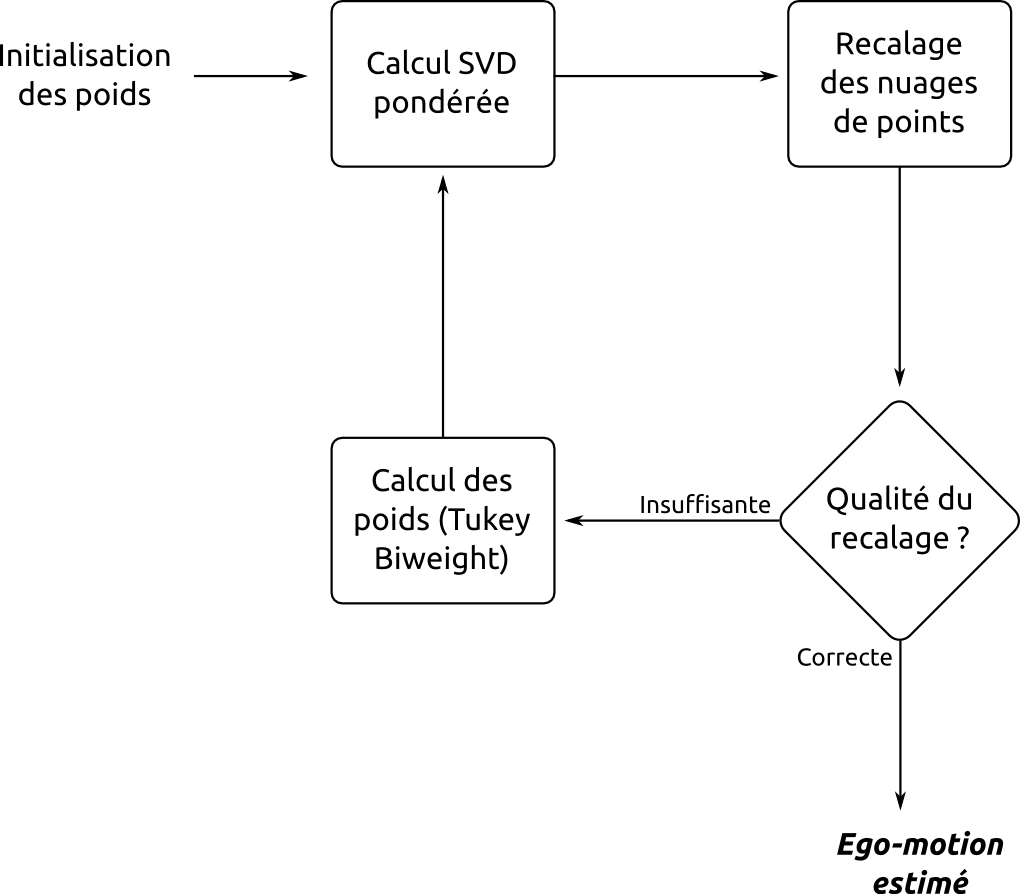
\includegraphics[width=0.7\textwidth]{Chapter4/graphics/overall_scheme_ego.png}
	\caption{Algorithme proposé pour estimer l'\textit{ego-motion} à partir des nuages de points}
	\label{fig:ch4_estimation_ego_motion}
\end{figure}

\subsubsection{Filtrage de l'ego-motion par UKF}
\paragraph{Pourquoi filtrer ?\\}
L'estimation de l'ego-motion présentée dans \ref{sec:ch4_robust_estimation} consiste en une optimisation locale, dans le sens où elle ne prend en compte que les deux dernières acquisitions pour calculer le déplacement. Nous avons vu précédemment (section \ref{sec:ch4_state_of_art_VO}) que plusieurs méthodes étaient possibles. Une optimisation sur plusieurs acquisitions consécutives \cite{Nister2006, Lategahna, Konolige2008} est une possibilité, mais il est également possible d'envisager un filtrage de nos observations pour obtenir la prise en compte de notre historique de mesure dans chaque nouvelle estimation (cf. figure \ref{fig:ch4_pourquoi_filtrer}). Nous retrouvons ici la dualité filtrage/optimisation présente dans de nombreuses approches de SLAM. Dans l'hypothèse où notre système est Markovien de rang 1 (hypothèse forte qui n'est pas nécessaire pour une approche d'optimisation multi-acquisitions), la littérature consacre de nombreux filtres à même d'estimer un ego-motion optimal.\\

Il s'agit de l'approche que nous avons retenue, du fait de la légèreté des nombreux filtres disponibles, de son intégration efficace dans un environnement multi-capteurs, et des performances obtenues qui nous ont semblé suffisantes. Une approche par optimisation est toujours possible, et serait peut-être à développer dans des travaux futurs, notamment en fonction de la puissance de calcul disponible sur la plate-forme embarquée choisie.\\

Il ne s'agit pas ici de réaliser un état de l'art des différents algorithmes de filtrage présents dans la littérature, tant ceux-ci sont nombreux et complexes. On introduit cependant dans les prochains paragraphe la solution que nous avons retenue, tout en présentant quelques éléments de choix qui ont prévalu.

\begin{figure}
	\centering
	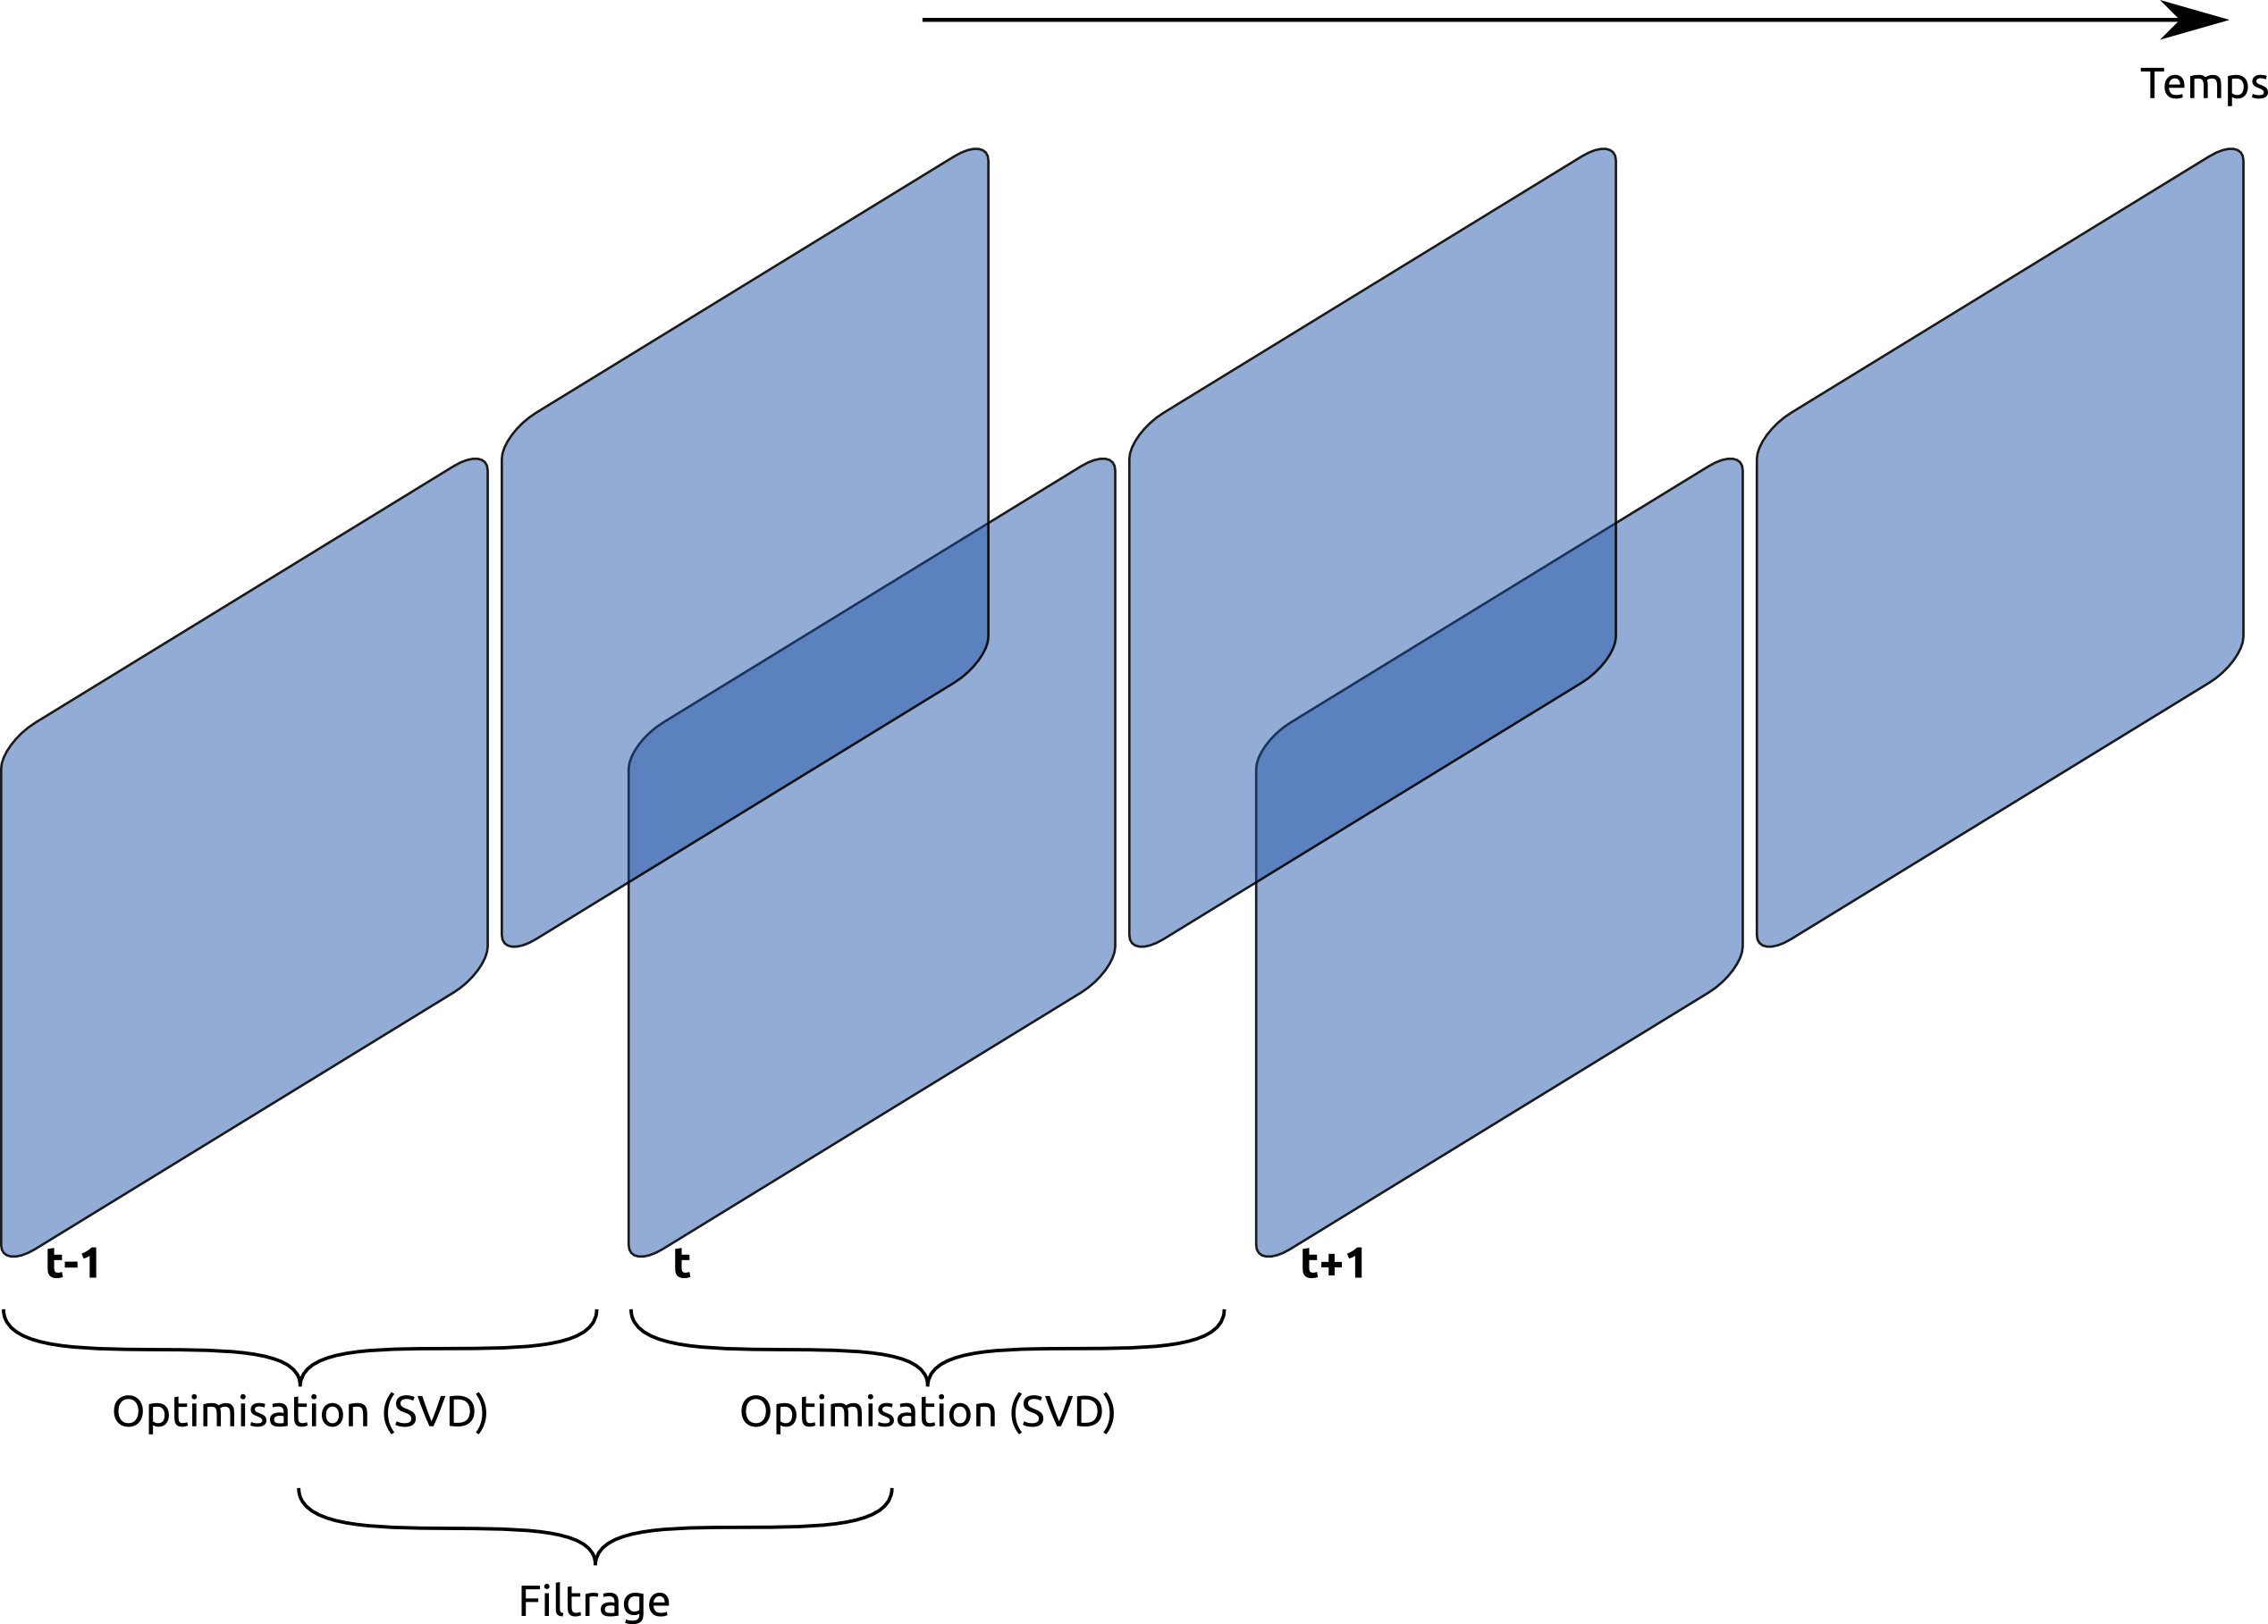
\includegraphics[width=0.8\textwidth]{Chapter4/graphics/why_filter.png}
	\caption{Illustration de l'apport du filtrage en termes de nombre d'acquisitions prises en compte}
	\label{fig:ch4_pourquoi_filtrer}
\end{figure}

\paragraph{Quel type de filtre choisir ?\\}
Comme nous l'avons détaillé dans \ref{sec:ch4_filtrage}, de nombreux algorithmes de filtrage sont présents dans la littérature, parmi lesquels le filtre de Kalman et quelque unes de ses variantes. Celui-ci est tout d'abord limité à des fonctions de propagation et de mesure linéaires, ce qui est en pratique très contraignant dans de nombreuses utilisations. L'estimation de la position courante à partir d'odométrie visuelle couplée à un système GPS ou à une centrale inertielle implique par exemple des fonctions non-linéaires lors des changements de référentiel. La fusion de données de positions relatives dans le cadre d'une collaboration entre véhicules est un autre exemple de mesure potentiellement non-linéaire.\\

Nous n'avons pas mis en œuvre de tel couplage dans le cadre de cette thèse, mais avons néanmoins choisi d'implémenter une solution l'autorisant dans un avenir proche. Ceci implique donc d'envisager les extensions EKF et UKF au filtre de Kalman, toutes deux capables de prendre en compte des fonctions de mesure linéarisables.\\

L'estimation de la position angulaire est ensuite rendue complexe par des singularités, si les angles sont paramétrés par les angles d'Euler. Les quaternions (introduits dans la section suivante) offrent une représentation plus simple à cet égard, et leur implémentation est rendue plus facile dans un UKF de par les points Sigma et l'absence du calcul de Jacobien (voir notamment \cite{Kraft2003}).\\

Nous avons choisi de nous concentrer sur le filtre de Kalman inodore, pour sa (relative) simplicité dans la gestion de fonctions de mesure et de propagation fortement non-linéaires, et ses performances supérieures à l'EKF dans ces cas de figure. 

\paragraph{Filtrage par Kalman inodore:\\}
Nous avons donc implémenté un algorithme de type UKF, avec un modèle de mouvement à vitesse constante (qui ne tient donc pas compte du mouvement non-holonomique des véhicules roulants usuels). Ce filtre utilise une représentation des angles par quaternions, qui permet de se prémunir simplement des singularités présentes dans une représentation eulérienne. Les quaternions sont une extension des nombres complexes classiques (qui autorisent notamment le paramétrage d'une rotation dans un plan), présents dans l'ensemble $\mathbb{H}$ homogène à $\mathbb{R}^4$, souvent représentés par leurs éléments de base \emph{(1,i,j,k)}, qui vérifient :

\begin{align}
	i^2 &= j^2 = k^2 = ijk = -1 \\
	q &= q_0 + q_1 \cdot i + q_2 \cdot j + q_3 \cdot k \qquad | \qquad \{q_k\}_{k \in [0..3]} \in \mathbb{R}
\end{align}

Les quaternions représentant une rotation sont restreints à $\mathbb{H}_1$, qui décrit les quaternions unitaires :

\begin{equation}
	\lVert q \rVert = \sqrt{q_0^2 + q_1^2 + q_2^2 + q_3^2} = 1
\end{equation}

La représentation des rotations en trois dimensions dans l'espace des quaternions unitaires ne souffre pas de singularités, ce qui simplifie grandement les étapes de propagation ou de mise à jour de l'estimation angulaire. La génération des points sigma de la transformation inodore est cependant un peu plus complexe, un exemple de procédé étant par exemple décrit dans \cite{Kraft2003}. \\
On pourra retenir que cette représentation n'est pas à proprement parler nécessaire dans le cas d'un filtrage du mouvement seul, les vitesses angulaires n'étant \textit{a priori} jamais proches des points $\pi$ ou $-\pi$. Cette représentation devient cependant très commode dès lors que l'on couple notre estimation avec un capteur de position angulaire, et que l'on cherche à estimer la position courante.


\subsection{Filtrage du nuage de points statiques échantillonné dans le temps} \label{sec:ch4_filtrage_nuage}
\subsubsection{Matrice de visibilité} \label{sec:ch4_matrice_visibilité}
On définit tout d'abord une matrice de visibilité, permettant de gérer les apparitions et disparitions successives des points observés. On se place ici dans une approche différente de la plupart des techniques présentées précédemment : l'enjeu, pour nous, est d'être capable de gérer en temps réel un nombre sensiblement constant de points d'intérêt répartis sur l'image, afin d'être à tout moment capable de détecter d'éventuels obstacles. La matrice de visibilité nous permet de rendre compte de l'observabilité des points lors des acquisitions successives, un point perdu lors d'une étape de suivi n'étant par ailleurs jamais réintroduit sous la même forme. La visibilité $V_{i,k}$ du point $i$ lors de l'acquisition $k$ vaut 1 lorsque ce point est le même que lors de l'acquisition $k-1$. S'il est perdu au cours de l'acquisition $k$, $V_{i,k}$ vaut 0 et un nouveau point est introduit avec la procédure décrite dans \ref{sec:ch3_Sélection dynamique des points d'intérêt}. De plus, chaque nouvelle acquisition conduit à un décalage de la matrice de visibilité, les acquisitions trop anciennes ne sont plus prises en compte. Une illustration de cette indexation est présentée sur la figure \ref{fig:ch4_visibility_matrix};

\begin{figure}
	\centering
	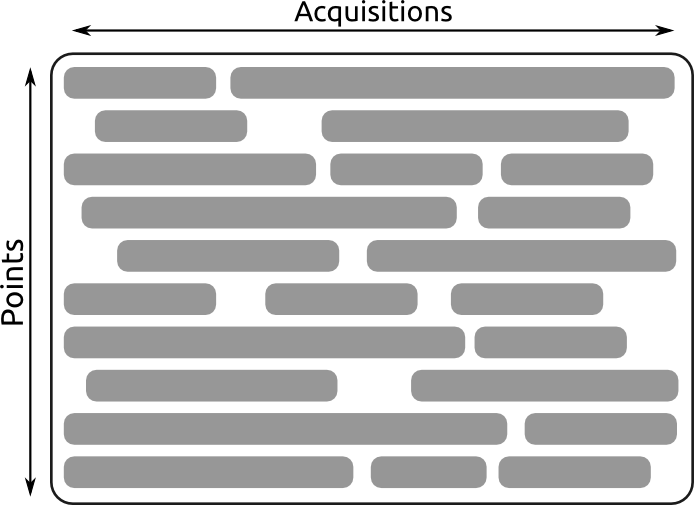
\includegraphics[width=0.6\textwidth]{Chapter4/graphics/visibility_matrix.png}
	\caption{Représentation schématique de la matrice de visibilité}
	\label{fig:ch4_visibility_matrix}
\end{figure}

\subsubsection{Filtrage des points} \label{sec:ch4_filtrage_des_points}
% Plusieurs observations du même point
\paragraph{Observations multiples:\\}
Chaque paire d'image conduisant à l'acquisition d'un nuage de points dans le référentiel du porteur, la détermination de l'ego-motion permet de s'affranchir de ces différences et de ramener toutes les acquisitions dans le même repère. Le suivi de points s'étant par ailleurs effectué dans le temps, on dispose potentiellement pour chaque élément physique observé de nombreuses observations. Le nombre de nuages de points conservés en mémoire tampon (de l'ordre de 200 nuages pour une fenêtre d'intégration de 10 s dans le cas de caméras à 20 images/s) reste le facteur limitant. Il s'agit alors d'obtenir un unique modèle décrivant l'environnement, et d'estimer la meilleure position de chacun de ces éléments.\\

% Optimisation ou filtrage ?
\paragraph{Optimisation ou filtrage:\\}
Deux approches sont alors possibles, comme présenté dans la section \ref{sec:ch4_state_of_art}. Nous pouvons exploiter un algorithme d'optimisation globale appliqué sur une fenêtre glissante (appelé \textit{ajustement de rayons} dans la littérature), ou bien utiliser un estimateur approprié pour obtenir la position de chacun des points. Strasdat \textit{et al.} (\cite{Strasdat2012}) préconisent une approche par filtrage, ce mécanisme assurant pour un coût constant au cours du temps (à nombre de points positionnés égal) la prise en compte de l'ensemble des observations. Une approche par optimisation ne peut prendre en compte l'ensemble des observations et fonctionner en temps constant. Les algorithmes proposés dans la littérature fonctionnent donc souvent sur une fenêtre glissante (seules les observations les plus récentes sont prises en compte, ou bien par sélection d'observations principales (voir par exemple Klein et Murray \cite{Klein2007}, Strasdat \textit{et al}. \cite{Strasdat}, Mei \textit{et al.} \cite{Mei2010})). L'usage d'un estimateur par point apparaissant comme moins coûteux et suffisant en termes de performances, il s'agit de l'approche que nous avons retenue. Il serait cependant possible d'implémenter une solution basée sur un ajustement de rayons pour améliorer la reconstruction de l'environnement à grande échelle, dans un futur développement.

\paragraph{Choix d'un estimateur:\\}
% Filtrage : quel estimateur choisir ? 
Lategahn \textit{et al.} \cite{Lategahn2011} proposent d'utiliser un filtre de Kalman pour estimer individuellement la position des points observés. Les mesures par stéréo-vision sont alors la seule entrée de cet algorithme, qui suppose le point statique et le bruit de position indépendant sur les trois dimensions considérées. Ce filtre revient, dans ce cas, à positionner les points au prorata de la variance de l'estimation et des mesures. Cette approche est relativement coûteuse, eût égard au nombre de points à positionner, et nous avons choisi une estimation plus rapide, que nous supposons suffisante et finalement assez proche en termes de performances. On considère en effet que l'estimation précise du bruit de mesure est de fait un élément difficile des algorithmes de stéréo-vision (fonction du bruit de corrélation entre deux éléments visuels, il n'est pas nécessairement constant et dépendra sans doute de l'environnement visuel du point positionné). Dans ce cadre, nous avons supposé que la plus-value apportée par un filtre de Kalman individuel n'était pas pertinente, et qu'un estimateur plus simple était possible.

\paragraph{Algorithme proposé:\\}
% Notre proposition
L'estimation de la position des points diffère selon deux critères : le points est-il statique ou mobile, est-il encore visible ou non ? Dans le premier cas, on propose d'estimer la position des points par une moyenne pondérée par la distance entre l'élément physique et le plan image lors de l'observation (formulation détaillée dans \ref{eq:ch4_filtrage_pose_points}). Dans ce cas, les points encore visibles sont constamment ré-estimés à chaque nouvelle acquisition, tandis que les points qui ne sont plus visibles sont figés dans un nuage de point statique, que l'on ramène à chaque itération dans le référentiel courant. Si le point est détecté comme un point mobile, selon la méthode précisée dans \ref{sec:ch5_Détection_candidats}, on reporte seulement la position moyennée selon les trois dernières observations. La pondération par la distance lors de l'observation ne rend pas exactement compte de l'ellipse d'incertitude liée au passage dans l'espace en trois dimensions, mais elle nous permet d'en approximer l'amplitude à moindre coût.\\

% Algo
On note dans ce qui suit $X_i^k = (x_i^k, y_i^k, z_i^k)$ le vecteur décrivant la position du point $k$ à l'itération $i$ dans son référentiel courant. On note $X_{j,i}^k$ la position du même point telle qu'observée lors de l'itération $j$ mais ramenée dans le référentiel du porteur lors de l'itération $i$. On note enfin $R_{i,j}$ et $T_{i,j}$ les matrices de transformation permettant de passer du référentiel du porteur lors de l'itération $j$ à celui de l'itération $i$. L'estimation de la position observé depuis l'itération $j$ lors de l'itération $i$ s'écrit alors :

\begin{align}
	X_{j,i}^k	 	&= [R_{i,j} | T_{i,j}] X_j^k \\
	{\hat{X^k}} &= \frac{1}{\nabla} \sum\limits_{l = j}^{i} \frac{X_{l,i}^k}{z_{l}^k}  \label{eq:ch4_filtrage_pose_points}\\
	\nabla 			&= \sum\limits_{l = j}^{i} \frac{1}{z_{l}^k}
\end{align}

La méthode proposée implique de parcourir, pour chaque nouvelle acquisition, l'ensemble des observations passées des points encore visibles pour calculer leur nouvelle position estimée. Ces calculs sont redondants, et le choix d'un estimateur récursif tel qu'une moyenne exponentielle\footnote{Moyenne exponentielle : pour une fenêtre d'intégration de taille $l$, sa valeur est calculée récursivement par: $\hat{X_{l,k}} = \alpha X_k + (1-\alpha) \hat{X_{l,k-1}}$. Le coefficient $\alpha$ est fixe, et vaut: $\alpha = \frac{2}{l + 1}$ } pourrait améliorer le temps de calcul. Le problème de cette méthode serait d'accorder une confiance aux observations fonction du temps, qui n'est pas nécessairement corrélée au réel bruit d'observation (si le porteur s'écarte d'un élément fixe par exemple, le bruit d'observation va croissant). L'utilisation d'un autre estimateur récursif serait peut être possible, bien que la sortie des observations de la mémoire tampon soit à prendre en compte. Ce sujet mériterait certainement des travaux complémentaires.

\section{Implémentation et évaluation} 
\subsection{Ego-Motion}\label{sec:ch4_eval_ego_motion}
Le calcul de l'ego-motion a été implémenté en C++, en utilisant la librairie Eigen\footnote{librairie open-source de calcul matriciel. Pour plus d'informations voir http://eigen.tuxfamily.org} pour le calcul matriciel et l'usage des quaternions. Le temps de calcul est très faible par rapport au reste de notre algorithme, comme présenté dans \ref{sec:ch4_temps_de_calcul}, et approximativement constant.

\subsubsection{Base de données utilisée}
On se base dans la suite sur les données du jeu de données KITTI (\cite{Geiger2012}), qui fournit une vérité terrain à base de centrale inertielle et de GPS. Les acquisitions d'images sont réalisées par des caméras \textit{Point Grey}, à la cadence relativement basse de 10 paires d'images par seconde. La plate-forme d'enregistrement est un véhicule automobile, ce qui explique les vitesses de déplacements relativement élevées pour notre méthode, pouvant monter jusqu'à 10m/s. Les acquisitions représentent un environnement urbain (dans la ville de Karlsruhe) mais aussi des voies rapides.

\subsubsection{Apport de l'UKF}
On évalue tout d'abord l'apport de l'algorithme de filtrage UKF dans la détermination de l'ego-motion, en représentant tout d'abord sur la figure \ref{fig:ch4_egomotion_ukf_raw} les estimations incrémentales du déplacement sur un axe au fil du temps, obtenues de manière brute et après le filtrage proposé comme intégration temporelle.

\begin{figure} 
	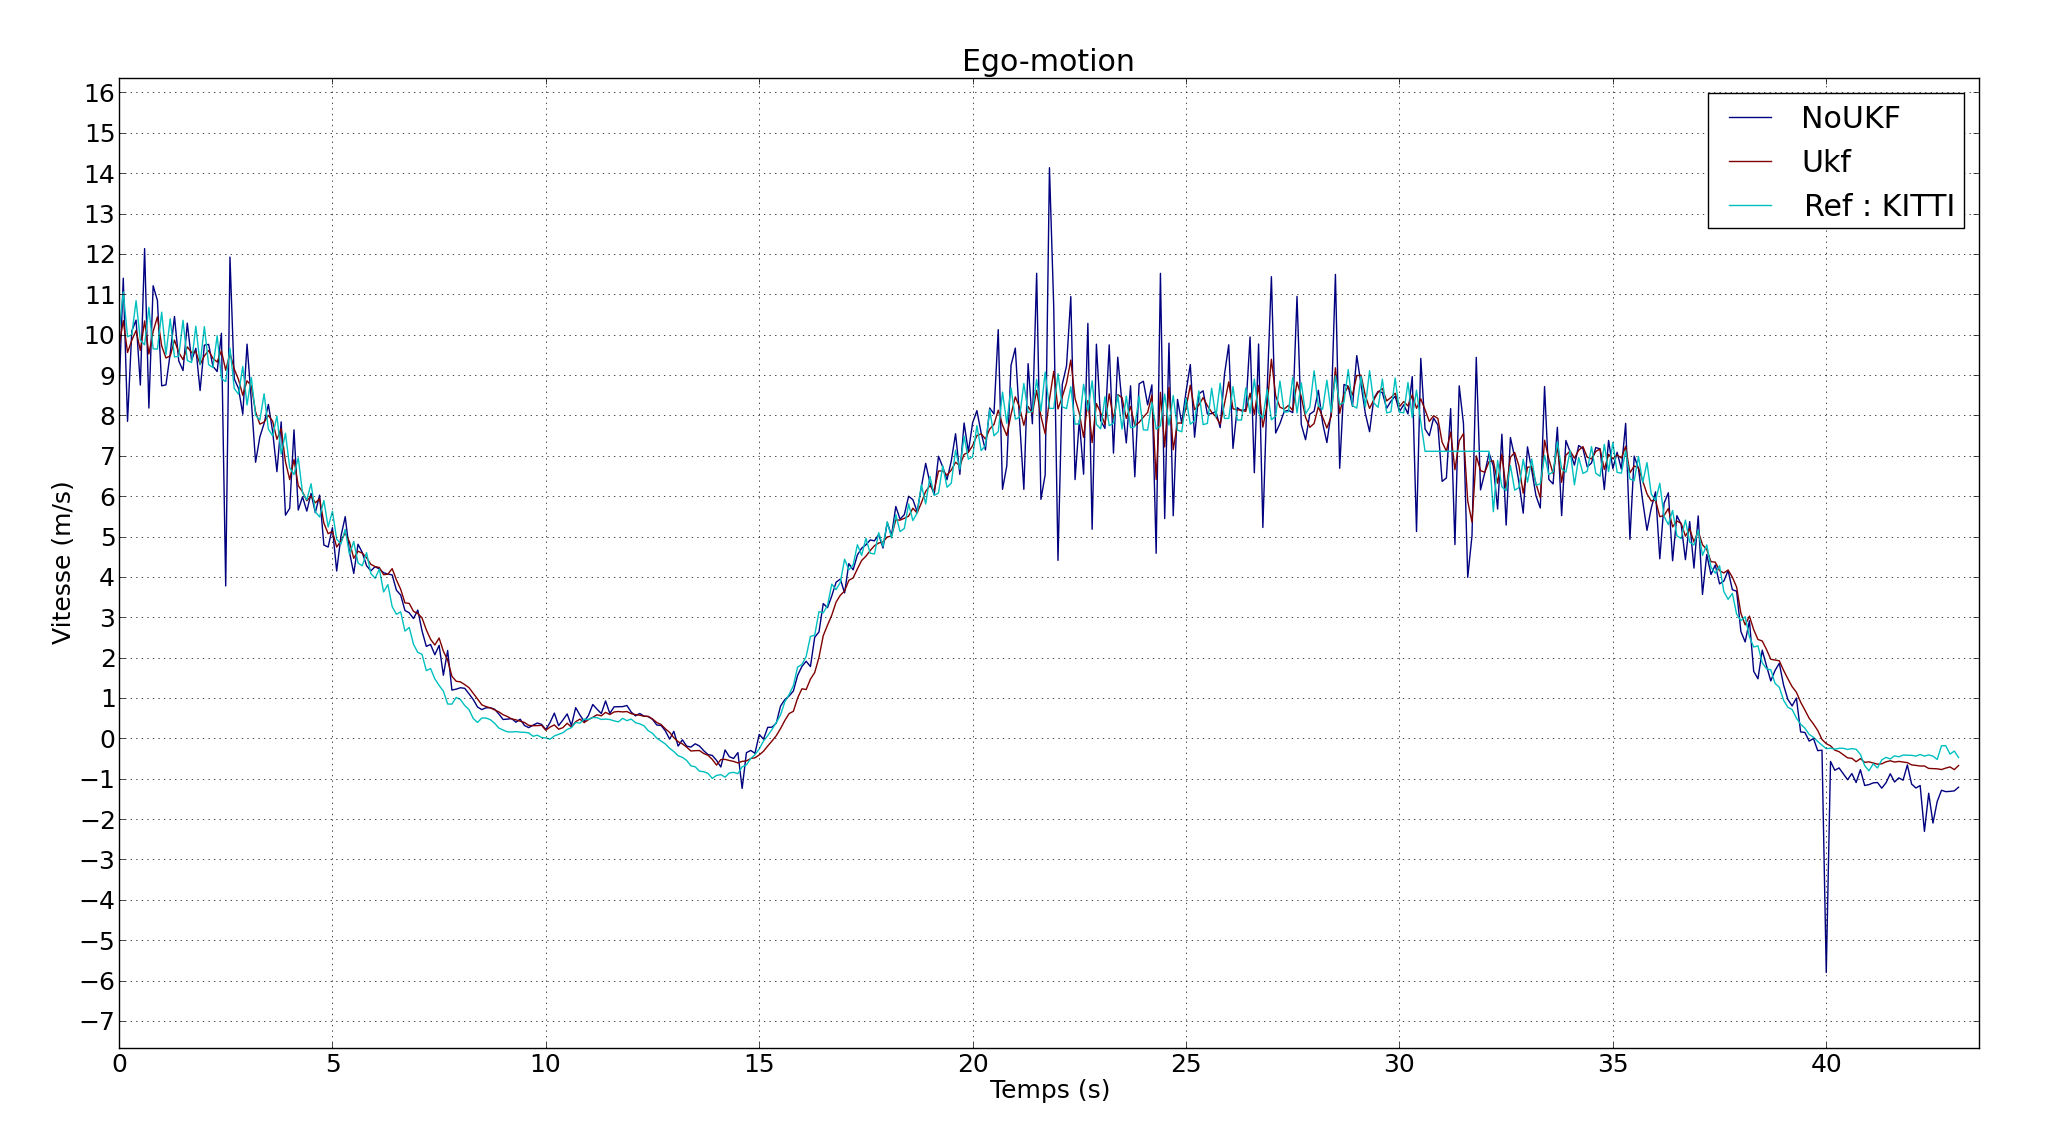
\includegraphics[width=\textwidth]{Chapter4/graphics/ego_motion_UKF_RAW.png}
	\caption{Précision de la détermination de l'ego-motion - comparaison des performances brutes et filtrées. La vitesse est mesurée sur un axe fixe (référentiel initial).}
	\label{fig:ch4_egomotion_ukf_raw}
\end{figure}

On constate aisément que l'estimation du mouvement bénéficie grandement du filtrage proposé en termes de bruit, son coût calculatoire étant, par ailleurs, très faible dans notre implémentation. Les erreurs d'estimation très importantes liées à des mouvements brusques, visibles sur les estimations \og brutes\fg{} sont bien pris en compte par le filtrage, et l'\textit{ego-motion} filtré est qualitativement de qualité très supérieure.\\

\subsubsection{Qualité de l'estimation : comparaison avec l'état de l'art}
On évalue ensuite les performances de notre approche de détermination du mouvement en termes de qualité de positionnement. On se place dans les conditions d'une navigation à l'estime, c'est-à-dire que l'estimation du mouvement propre est la seule information utilisée pour reconstruire les positions successives. \\
Les erreurs de détermination d'angle de rotation conduisent à une erreur de position s'accroissant avec la distance parcourue, phénomène connu sous le nom d'erreur d'Abbe. Les erreurs dans la détermination de la translation sont en général moins influentes, car elles conduisent à une erreur dans le positionnement qui se répartit comme le résultat d'une marche aléatoire, de moyenne nulle dans le cas d'erreurs non-biaisées et qui augmente au fil du temps la largeur de la distribution des positions. \\

\paragraph{Trajectoire obtenue par une marche à l'estime:\\}
La méthode proposée ne comporte pas d'optimisation globale de la trajectoire, qui serait notamment à même d'exploiter une détection des fermetures de boucles. La dérive de la position estimée augmente donc constamment, comme on peut le constater sur la figure \ref{fig:ch4_deadreckoning_overall}. La trajectoire représentée est longue d'environ 1,6 km, très au delà de nos besoins en termes de fenêtre d'intégration (elle représente la trajectoire cumulée observée sur 1900 paires d'images). On utilise un repère orthonormé dont l'origine est le point de départ de la navigation à l'estime.

\begin{figure}[h]
		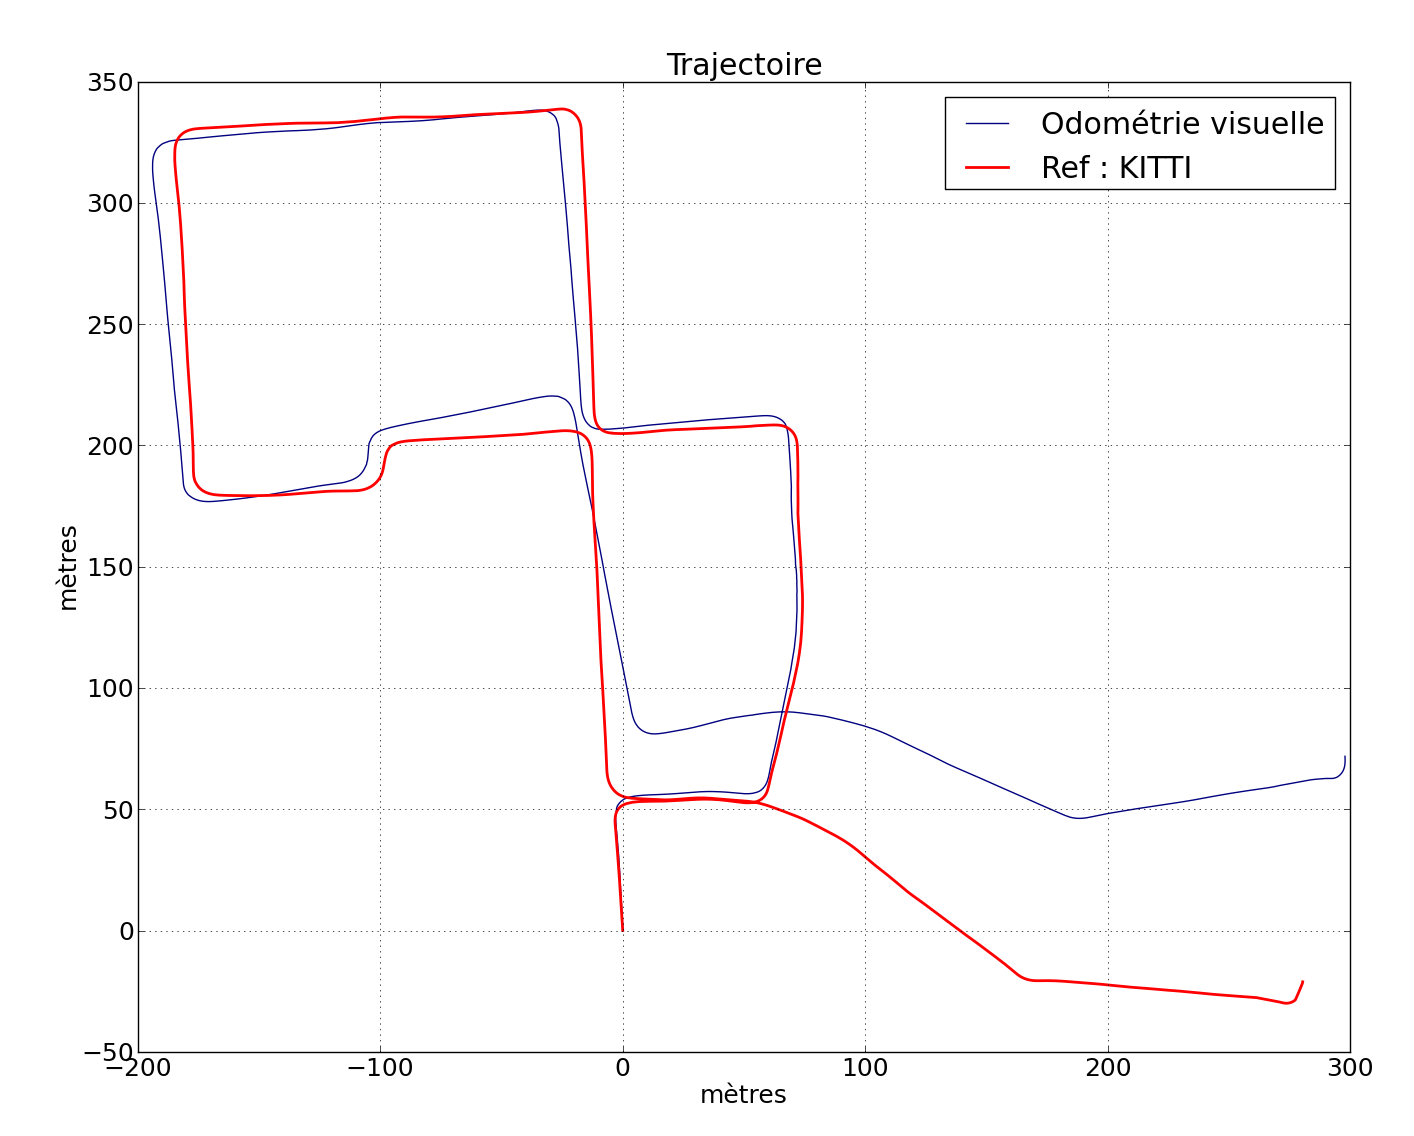
\includegraphics[width=\textwidth]{Chapter4/graphics/dead_reckoning_overall.png}
		\caption{Exemple de navigation à l'estime et de sa dérive cumulée (KITTI - séquence 1). Le point (0,0) constitue le point de départ de la marche à l'estime.}
		\label{fig:ch4_deadreckoning_overall}
\end{figure}

\paragraph{Évaluation quantitative:\\}
L'estimation de la qualité de l'ego-motion demande cependant une représentation plus complète, les résultats obtenus par une comparaison directe des trajectoires de deux méthodes pouvant être trompeurs. L'erreur d'Abbe n'étant pas uniformément répartie en fonction de la distance parcourue, différents points de départ peuvent en effet conduire à des performances \emph{a priori} très différentes. Il est ainsi d'usage de représenter l'erreur en fonction de la distance parcourue, mais en considérant un grand nombre de points de départs possibles sur une séquence donnée, et en moyennant les résultats. On présente donc sur la figure \ref{fig:ch4_error_over_distance} l'erreur de position obtenue par une navigation à l'estime, fonction de la distance parcourue, moyennée sur l'ensemble des tronçons de 400 mètres présents sur la première séquence de la partie \og odométrie\fg{} du jeu de données KITTI (par pas de 10 m, soit environ 150 tronçons). Les interpolations nécessaires sont réalisées de manière linéaire. Le profil observé s'explique par les erreurs de translation et de rotation, qui n'ont pas la même évolution en fonction de la distance parcourue. L'erreur de translation est en effet immédiatement visible, tandis qu'une erreur de rotation n'a initialement qu'un effet limité. L'accumulation des déplacements dans un référentiel erroné en termes de rotation conduit cependant à une erreur fonction croissante de la distance, qui devient donc à terme dominante.

\begin{figure} 
	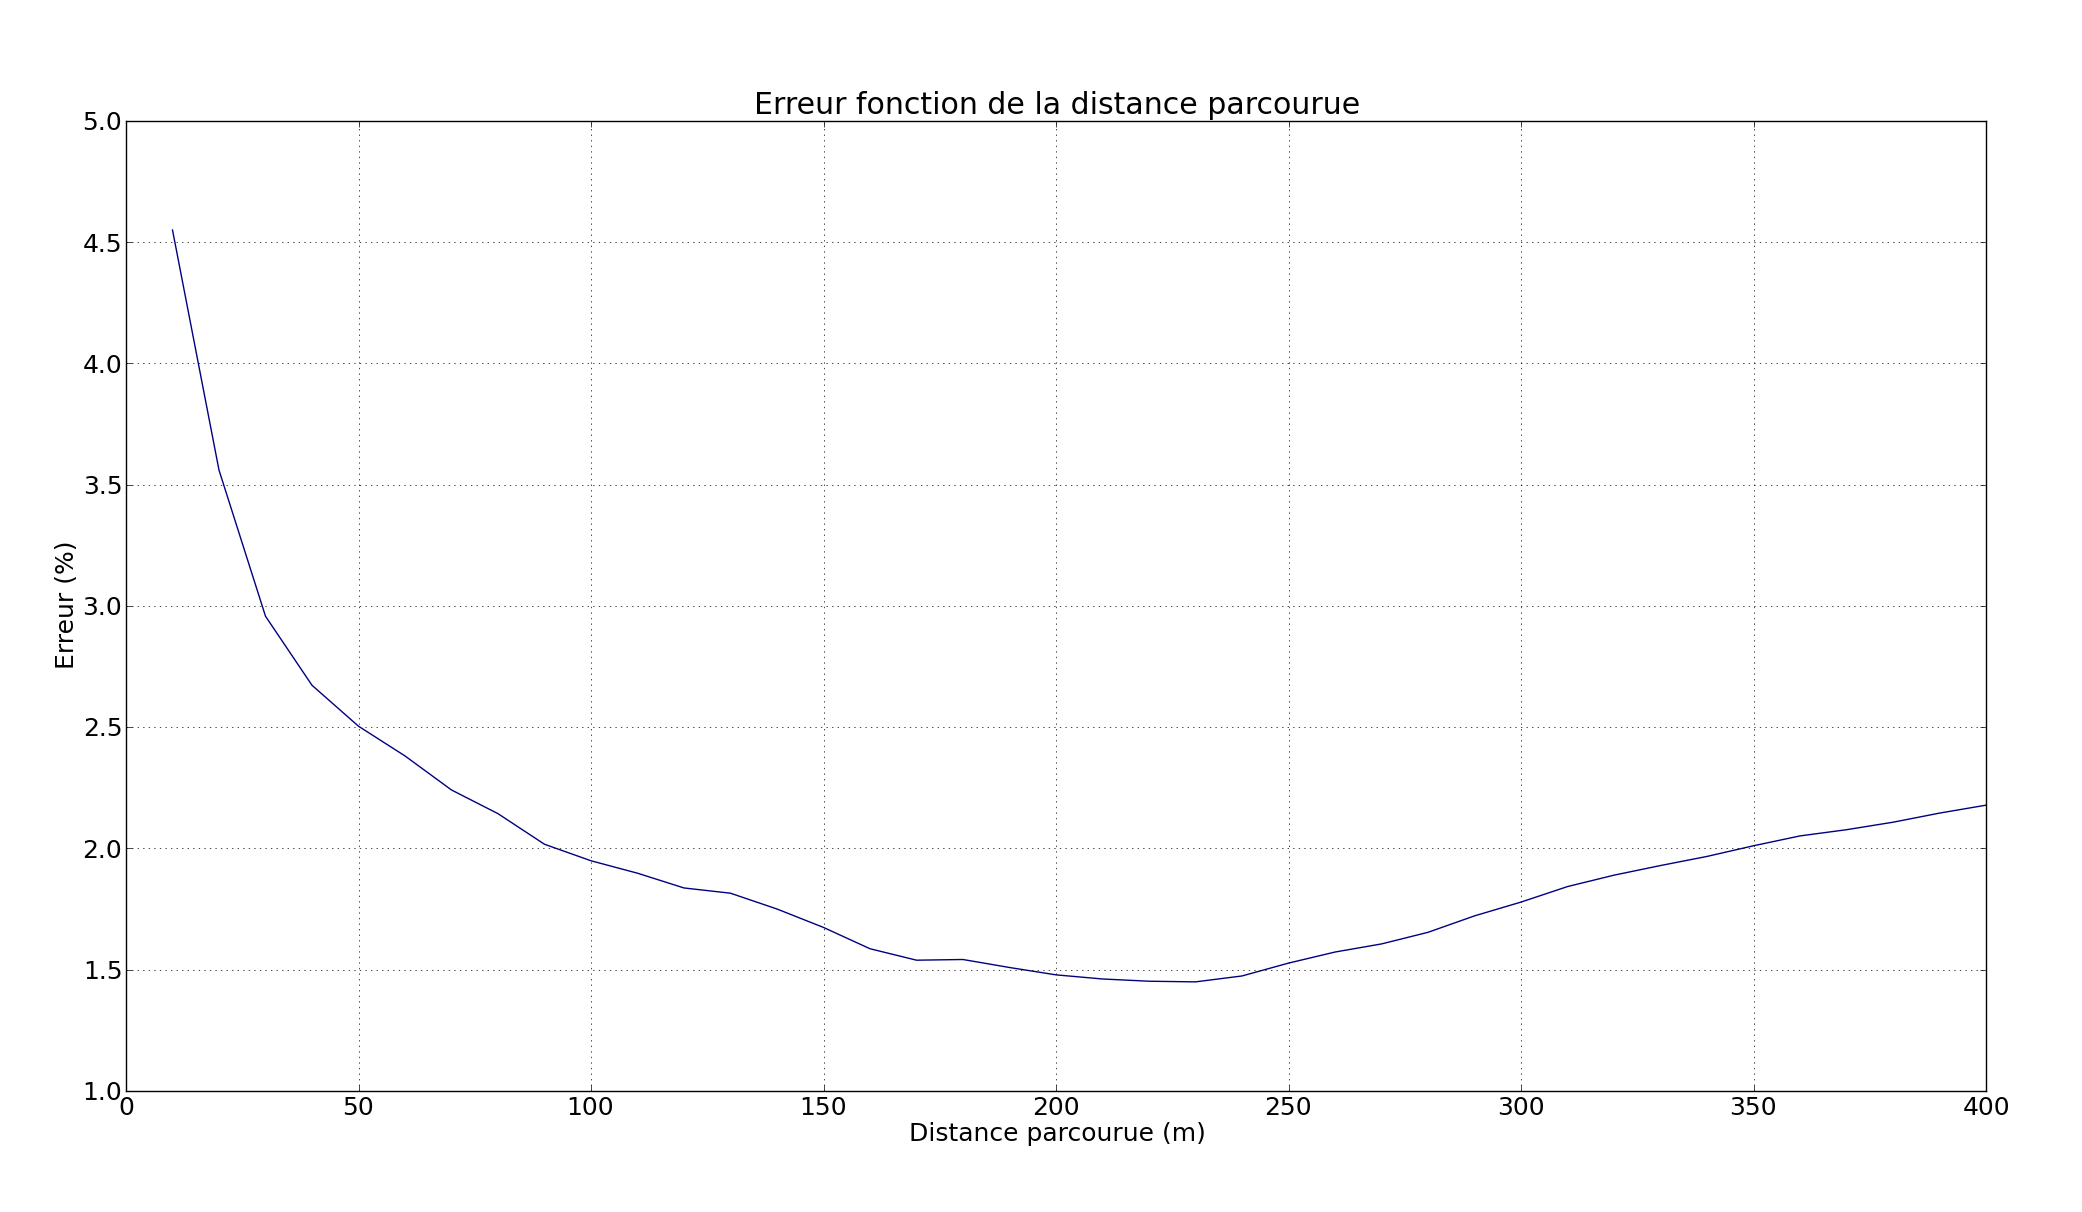
\includegraphics[width=0.8\textwidth]{Chapter4/graphics/error_over_distance_-_sliding_window.png}
	\caption{Erreur de positionnement fonction de la distance parcourue sur l'ensemble des tronçons de 450m possibles (KITTI - séquence 1)}
	\label{fig:ch4_error_over_distance}
\end{figure}

Ces performances sont à comparer à l'état de l'art, et l'on reprend dans le tableau \ref{tab:ch4_résultats_kitti} les résultats présents sur le site de KITTI (\cite{KIT}). Le temps de calcul doit prendre en compte le suivi de points présenté dans le chapitre précédent, et la détermination de l'egomotion que nous présentons ici. Cette dernière est très rapide, comme attendu, puisque qu'elle demande environ 2 ms sur un processeur Intel Core i7 à 2GHz (un seul coeur étant nécessaire). Le suivi de 4000 points sur une plate-forme comparable (CPU donc) demande quant à lui de l'ordre de 45 ms dans les mêmes conditions (suivi de 4000 points).\\

On ne considère cependant ici que la première des séquences proposées par ce jeu de données, contrairement aux autres évaluations présentes dans le tableau, le classement présenté l'étant à titre indicatif. La méthode proposée n'a pas vocation à améliorer l'état de l'art en matière d'odométrie visuelle, ce problème dépassant de loin la problématique de cette thèse qui est axée sur la perception de l'environnement. \\

\begin{table}
	\resizebox{13cm}{!}{
		\centering {
			\begin{tabular}{c | c | c | c | c | c}
				{\bf Classement} & {\bf Méthode} & {\bf Err. Translation} & {\bf Err. Rotation} & {\bf Temps de calcul} & {\bf Plate-forme}\\ \hline
				1 & VoBa 												& 1.77 \% 	& 0.0066 [deg/m] & 0.1 s 	& 1 core @ 2.0 Ghz (C/C++)\\
				2 & VISO2-SAM 									& 1.83 \% 	& 0.0152 [deg/m] & 0.05 s 	& 1 core @ 3.5 Ghz (C/C++)\\
				3 & MFI 												& 1.84 \% 	& 0.0070 [deg/m] & 0.1 s 	& 4 cores @ 3.0 Ghz (C/C++)\\
				4 & eVO 												& 1.93 \% 	& 0.0076 [deg/m] & 0.05 s 	& 2 cores @ 2.0 Ghz (C/C++)\\
				-- & \textbf{Solution proposée} 	& \textbf{1.9 \%} & \textbf{0.015} &  \textbf{0.05s}		&  \textbf{4 cores @ 2.0GHz (C++)}\\
				5 & D6DVO 											& 2.10 \% 	& 0.0083 [deg/m] & 0.03 s 	& 1 core @ 2.5 Ghz (C/C++)\\
				6 & GT\_VO3pt 									& 2.21 \% 	& 0.0117 [deg/m] & 1.26 s 	& 1 core @ 2.5 Ghz (C/C++)\\
				7 & VISO2-S 	& 2.27 \% 				& 0.0152 [deg/m] & 0.05 s 	& 1 core @ 2.5 Ghz (C/C++)\\
				8 & BoofCV-SQ3 	& 2.27 \% 			& 0.0111 [deg/m] & 0.14 s 	& 1 core @ 2.5 Ghz (Java)\\
				9 & TGVO 		& 2.44 \% 					& 0.0105 [deg/m] & 0.06 s 	& 1 core @ 2.5 Ghz (C/C++)\\
				10 & SVO 		& 2.45 \% 					& 0.0109 [deg/m] & 0.05 s 	& 2 cores @ 2.5 Ghz (C/C++)\\
				11 & VO3pt 		& 2.93 \% 				& 0.0116 [deg/m] & 0.56 s 	& 1 core @ 2.0 Ghz (C/C++)\\
				12 & VO3ptLBA 	& 3.17 \% 			& 0.0180 [deg/m] & 0.57 s 	& 1 core @ 2.0 Ghz (C/C++)\\
				13 & KPnP 		& 3.46 \% 				& 0.0144 [deg/m] & 0.2 s 		& 1 core @ 2.5 Ghz (Matlab)\\
				14 & MSD VO 	& 3.50 \% 				& 0.0166 [deg/m] & 0.07 s 	& 1 core @ 2.8 Ghz (C/C++)\\
				15 & MLM-SFM 	& 4.07 \% 				& 0.0104 [deg/m] & 0.03 s 	& 5 cores @ 2.5 Ghz (C/C++)\\
				16 & VOFS 		& 4.21 \% 				& 0.0158 [deg/m] & 0.51 s 	& 1 core @ 2.0 Ghz (C/C++)\\
				17 & VOFSLBA 	& 4.35 \% 				& 0.0189 [deg/m] & 0.52 s 	& 1 core @ 2.0 Ghz (C/C++)\\
				18 & VISO2-M 	& 13.79 \% 				& 0.0372 [deg/m] & 0.1 s 		& 1 core @ 2.5 Ghz (C/C++)\\
			\end{tabular}
		}
	}	
	\caption{Résultats de différentes méthodes sur le jeu de données KITTI. Notre méthode n'est évaluée que sur la première séquence, contrairement aux autres résultats (11 séquences)}
	\label{tab:ch4_résultats_kitti}
\end{table}

\subsection{Reconstruction 3D}
La reconstruction de l'environnement a été également implémentée en C++, en utilisant là encore la librairie Eigen pour les calculs matriciels, et la structure \emph{PointCloud} de la librairie PCL (\emph{Point Cloud Library}, \cite{Rusu2011}) pour le stockage des nuages de points. Cette étape est également très rapide, étant essentiellement limitée dans le nombre de points traités par leur stockage en mémoire courante. \\
Une évaluation quantitative de la reconstruction est difficile, faute de vérité terrain aisément comparable, nous présentons donc une comparaison avec l'environnement obtenu par un capteur de type \emph{Velodyne}, le HDL64. La qualité de la reconstruction en trois dimensions est difficile à appréhender sur une projection, d'autant plus que la répartition des points diffère entre les deux procédés, mais on peut notamment remarquer que les plus gros obstacles (voitures, éléments de voirie) sont bien visibles sur le squelette reconstitué. Les nuages de points obtenus par ces deux procédés sont présentés sur la figure \ref{fig:ch4_comparaison_velodyne}. Le nuage de point \emph{Velodyne} correspond à une unique acquisition tandis que le nuage de points que nous présentons correspond à une intégration temporelle, l'objectif n'est donc pas d'évaluer les mérites respectifs de ces approches mais bien plus d'exploiter une vérité terrain obtenue par le télémètre laser.\\

\begin{figure}[h]
	\begin{center}
		\begin{subfigure}{1.0\textwidth}
			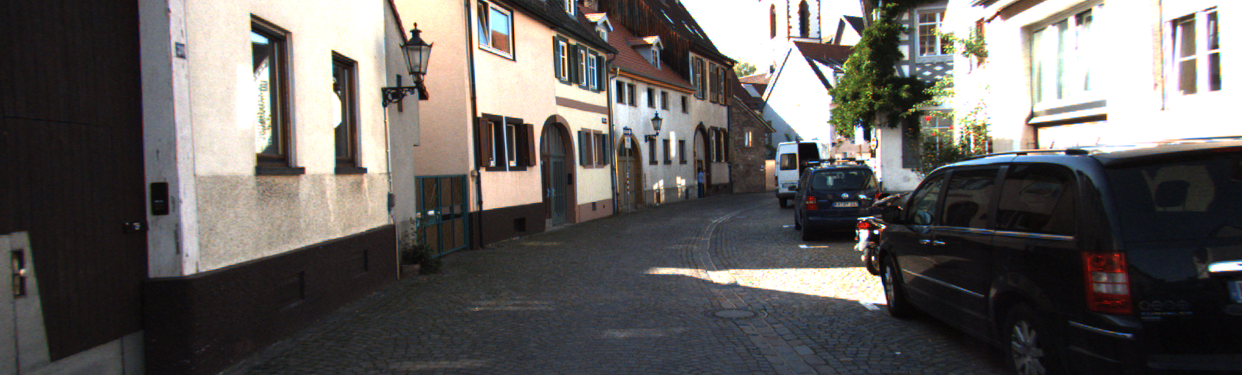
\includegraphics[width=\textwidth]{Chapter4/graphics/KITTI_pict.png} 
			\caption{Vue de la caméra}
		\end{subfigure}	
		\newline
		\begin{subfigure}[t]{0.48\textwidth}
			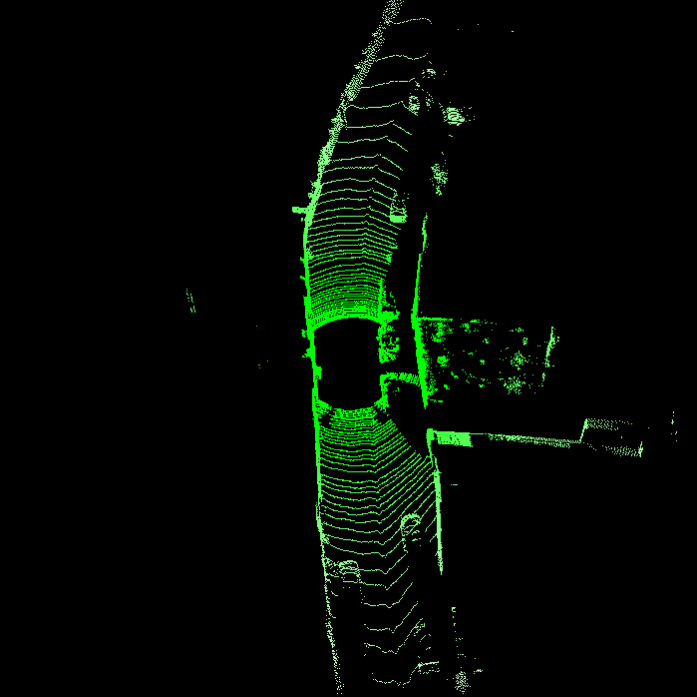
\includegraphics[width=\textwidth]{Chapter4/graphics/KITTI_Velodyne.png} 
			\caption{Nuage de points instantané du capteur HDL64. Vue aérienne}
		\end{subfigure}	
		~
		\begin{subfigure}[t]{0.48\textwidth}
			\includegraphics[width=\textwidth]{Chapter4/graphics/KITTI_SLAM_1.png} 
			\caption{Nuage de points obtenu par notre méthode, et trajectoire estimée du véhicule. Vue aérienne}
		\end{subfigure}	
		
		\caption{Comparaison des nuages de points obtenus par un télémètre laser Velodyne HDL64 (b) et par notre proposition (c)(Données issues de KITTI). Le temps de calcul décrit la période minimale entre deux acquisitions, et comprend l'ensemble des étapes  de l'algorithme (suivi de points dans l'image, estimation de l'ego-motion et reconstruction 3D dans notre cas).}
		\label{fig:ch4_comparaison_velodyne}
	\end{center}
\end{figure}

\subsection{Temps de calcul} \label{sec:ch4_temps_de_calcul}
La problématique du calcul temps réel est respectée sans trop de difficultés par cette étape de notre algorithme. Cette étape rajoute une latence qui reporte les étapes suivantes, mais ne restreint pas la cadence de traitement, dans la mesure où le suivi de points dans l'image reste le facteur limitant (cf. section \ref{sec:ch6_temps_reel}). Notre implémentation est réalisée en C++, avec l'aide de la librairie Eigen pour le calcul matriciel, et exploite plusieurs processus parallèles. La plate-forme de test utilise un processeur de type Intel Core i7 à 2GHz, les quatres unités d'exécution présentes étant utilisées.\\
On représente à la fois sur la figure \ref{fig:ch4_temps_de_calcul} l'évolution du temps de calcul et celle du nombre de points présents dans l'environnement modélisé. Le jeu de données utilisé est celui de KITTI (\cite{Geiger2012}), acquis depuis une plate forme automobile dans un environnement urbain. On maintient un ensemble de 4000 points suivis sur les paires d'images stéréoscopiques exploitées, 100 acquisitions étant ensuite prises en compte dans la construction du squelette représentatif de l'environnement. Du fait de la cadence d'acquisition de 10 images par seconde sur ce jeu de données, les 10 dernières secondes d'observation sont donc prises en compte dans l'environnement représenté.\\

\begin{figure}[h] 
	\centering
	\includegraphics[width=0.98\textwidth]{Chapter4/graphics/computing_time.png}
	\caption{Exemple d'évolution du temps de calcul global de cette étape (ego-motion et reconstruction de l'environnement). Les fluctuations s'expliquent en partie par une variation du nombre de points observés ou en mémoire.}
	\label{fig:ch4_temps_de_calcul}
\end{figure}

On peut remarquer sur la figure \ref{fig:ch4_temps_de_calcul} que le temps de calcul augmente en fonction du nombre de points présents, comme attendu. Tous les points présents n'ont cependant pas le même coût de propagation, la position des points encore visibles étant réévaluée à chaque nouvelle observation, tandis que les points qui ne sont plus visibles sont représentés par leur dernière position estimée, et simplement ramenés dans le référentiel courant (section \ref{sec:ch4_filtrage_des_points}). Les fluctuations constatées dans le temps de calcul sont alors liées à la sortie des points observés du champ de vision. Certains déplacements peuvent ainsi influer rapidement sur le nombre de points sortant du champ de vision (virages brusques par exemple), ce qui explique, au moins partiellement, les variations du temps de calcul observées. Le nombre de points présents dans le squelette est borné par le nombre de nuages conservés en mémoire tampon, de même que le temps de calcul. On constate aisément que celui-ci est compatible avec une cadence d'acquisition élevée (cette étape pouvant traiter plus de 30 acquisitions par seconde en moyenne).\\

\subsection{Quelle fenêtre d'intégration ?}
Nous souhaitons ici améliorer notre perception de l'environnement en cumulant les observations selon une fenêtre temporelle d'intégration, dont l'étendue est de l'ordre de 100 paires d'images. Cette fenêtre d'intégration est limitée par deux facteurs : une contrainte d'implémentation (augmenter sa taille a un impact - assez faible relativement à l'ensemble du procédé - sur le temps de calcul, et demande plus de place en mémoire), et une contrainte environnementale. Il est ainsi inutile de cumuler les observations sur une échelle de temps très supérieure au temps de présence des éléments suivis dans le champ de vision. Celui-ci varie en fonction du déplacement du véhicule et du déplacement des objets de la scène, son estimation est délicate, mais on constate empiriquement qu'une fenêtre temporelle de 10 secondes est bien supérieure au temps de présence effectif de la majorité des éléments du champ de vision.\\

Une remarque peut être faite en termes d'ordre de grandeur, pour valider notre accumulation temporelle d'informations. On peut en effet comparer l'erreur introduite dans la reconstruction de l'environnement par la marche à l'estime le long de la fenêtre d'intégration, par rapport aux erreurs typiques liées à une observation de stéréo-vision. En supposant une vitesse d'environ 10 m/s et une cadence d'acquisition de 10 im/s, pour rester dans les conditions de l'évaluation ci-dessus, l'erreur attendue par la navigation à l'estime pendant l'accumulation est de l'ordre de 2m\footnote{Il s'agit d'un cas extrême, et l'erreur est dans ce cas concentrée sur les points les plus lointains.}. Une erreur de 0.5 pixels dans la détermination de la position d'un élément de la scène sur le plan image, pour un point dont la disparité initiale est de 3 pixels et avec les conditions des mesures précédentes, conduit à une erreur dans son positionnement dans l'espace de 15m. Il s'agit bien sûr d'un  calcul très grossier, mais il illustre l'intérêt du filtrage dans le temps des observations, en dépit de l'erreur réalisée sur la compensation du mouvement.

\section{Conclusion}
On a présenté dans ce chapitre une solution originale de détermination de l'\textit{ego-motion} à partir de points suivis sur une paire stéréo-vision, à un coût calculatoire très faible. Cette solution est suffisamment précise pour l'intégration temporelle que nous effectuons, qui nous permet de reconstruire la position des points suivis au fil du temps et de réduire un bruit d'observation très important dans un dispositif de stéréo-vision. \\
Du fait de la séparation entre ces deux tâches, nous montrons également que le nombre de points traités  en temps réel peut être très important, de l'ordre de plusieurs dizaines de milliers de points sur une plate-forme mobile grand public. Un récapitulatif de ces différentes étapes est visible sur la figure \ref{fig:ch4_vue_ensemble_algo}.\\

On dispose à ce moment d'un modèle de la scène environnant le porteur, grâce à des points positionnés dans l'espace. Ce modèle ne vaut que pour les points statiques, les points détectés comme mobiles nécessitant alors un traitement plus approfondi.

\begin{figure}[h] 
	\centering
	\includegraphics[width=0.98\textwidth]{Chapter4/graphics/detailled_scheme.png}
	\caption{Vue d'ensemble de l'algorithme proposé.}
	\label{fig:ch4_vue_ensemble_algo}
\end{figure}


\chapter{Détection, localisation, suivi des objets mobiles} 
\label{sec:ch5}
\vspace{10pt}

\minitoc
\clearpage

% % % % % % % % % % % % % % % % % % % % % % % % % % % % %
% Détection, localisation et suivi des objets mobiles   %
% % % % % % % % % % % % % % % % % % % % % % % % % % % % %

\section{Introduction}
La détection, la localisation et le suivi des objets mobiles sont une évolution naturelle de la perception \og instantanée\fg{} de l'environnement ; et sont capitaux pour la navigation de véhicules autonomes. Considérer les obstacles sans prendre en compte leur caractère dynamique n'est en effet possible que lorsque leur vitesse est négligeable devant celle du porteur automatisé, ou à l'inverse si la vitesse de ce dernier est suffisamment faible pour réagir aux erreurs de planification de trajectoire qui peuvent survenir dans un environnement dynamique mal évalué.\\

Une des singularités de notre approche, découlant des procédés précédents (Chapitres \ref{sec:ch3} et \ref{sec:ch4}), est de disposer à cette étape d'un ensemble de points de vue important (lié à notre fenêtre d'intégration temporelle) décrivant les observations successives d'éléments quasi-ponctuels de la scène. Ces éléments sont par ailleurs nombreux à être observés, de l'ordre de plusieurs milliers.\\
Ces observations sont dépendantes du bruit d'observation et des positions effectives des obstacles, une première étape consiste donc à détecter parmi elles les points en mouvement. En supposant que les éléments mobiles de la scène sont supportés par des objets distincts, on s'attache ensuite à segmenter ces éléments individuels en ensembles dont le déplacement et la configuration spatiale sont cohérents. Afin d'approfondir la connaissance de la scène, nous essayons ensuite de rattacher cette segmentation aux objets mobiles précédemment suivis, afin d'en déduire une trajectoire suivie dans le temps. Cette dernière peut être une information importante pour les étapes ultérieures de contrôle et de planification de trajectoire, qui ne seront cependant pas traitées dans ce manuscrit. Une illustration du réseau bayésien sous-jacent est visible sur la figure \ref{fig:ch5_intro_bayesian_network}.

\begin{figure}
	\begin{center}
		\includegraphics[width=0.4\textwidth]{Chapter5/graphics/intro_bayesian_network.png}
	\end{center}
	\caption{Schéma du réseau bayésien permettant, à partir des points mobiles détectés (\textbf{Z}) et des objets segmentés qui en découlent (\textbf{B})} d'estimer itérativement les objets mobiles présents (\textbf{T}).
	\label{fig:ch5_intro_bayesian_network}	
\end{figure}

\section{État de l'art}
\subsection{Détection d'objets mobiles au sein d'un nuage de points}
La détection d'objets mobiles au sein d'un nuage de points est le plus souvent présente dans la littérature dans le cadre d'acquisitions par un télémètre laser. Les nuages des points alors obtenus n'ont pas les mêmes caractéristiques que ceux dont nous disposons à cette étape, étant plus précis et plus denses, au sens de notre définition initiale de la densité de perception (section \ref{sec:ch3_densité_informations}). Ces nuages ne contiennent cependant pas d'information d'association dans le temps, c'est-à-dire que les liens entre plusieurs observations d'un même point de l'espace ne sont pas connues. Cette correspondance peut être retrouvée dans sa globalité, dans le sens où on peut ramener différentes observations dans le même référentiel, par la connaissance exacte du mouvement entre deux acquisitions (ce qui implique souvent la présence d'une centrale inertielle et d'un système de type GPS), ou par le calcul de la correspondance la plus probable (par exemple en utilisant un algorithme de type \emph{ICP}). Ceci n'assure cependant pas de correspondance point-à-point.\\
Kalyan \textit{et al.} (\cite{Kalyan2010}) proposent de ne considérer que la composante de distance au capteur des observations, puis d'utiliser l'algorithme \emph{Mean-Shift}, proposé par Fukunaga et Hostetler \cite{Fukunaga1975}) pour segmenter les différentes régions de l'image obtenue. Les changements de distance au capteur pour un azimut donné sont alors détectés comme des objets mobiles. Les cibles segmentées sont ensuite introduites dans un algorithme de filtrage, le GM-PHD, que nous détaillerons par la suite (section \ref{sec:ch5_filtrage_des_cibles}). Azim et Aycard proposent de se baser sur une grille d'occupation, alimentée par un télémètre laser, pour y détecter les inconsistances dans le temps \cite{Azim}. Celles-ci sont supposées provenir d'objets mobiles, et représentent des cibles qui sont ensuite suivies dans le temps. \\
D'autres approches intégrées avec la reconstruction de l'environnement sont aussi présentes dans la littérature, sous le nom de SLAMMOT (voir notamment \cite{Wang2007, Vu2009}), et ont déjà été introduites dans la section \ref{sec:ch2_SLAMMOT_stereo}.

\subsection{Détection d'objets mobiles dans l'espace image, sur une plate-forme mobile}
De nombreux algorithmes existent pour détecter des objets mobiles à partir d'images acquises depuis une plate-forme statique, souvent basés sur une soustraction préalable de la partie constante de l'image \cite{Piccardi2004}. La détection d'objets mobiles à partir d'une plate-forme elle même en mouvement est bien sûr plus complexe, car il faut dissocier dans les variations de l'image la partie induite par le déplacement d'un mouvement autonome. Une étape préalable consiste donc souvent à estimer l'\emph{ego-motion}, à partir d'un flux optique dense ou du suivi de points clefs. Cette donnée n'est cependant pas suffisante pour dissocier les éléments de la scène ayant un mouvement indépendant des éléments statiques. Le flux optique d'éléments statiques de la scène dépend en effet de leur distance au plan image de la caméra, qui est \textit{a priori} inconnue.\\

Dumortier \textit{et al.} proposent de détecter tout d'abord dans l'image le plan sur lequel le véhicule se déplace, et d'en déduire le mouvement effectué par le véhicule \cite{Dumortier}. Ce mouvement est alors utilisé pour coupler des observations dans le temps, et permet de calculer une carte de profondeur (stéréo-vision temporelle), à partir de laquelle les obstacles peuvent être détectés. Agrawal \textit{et al.} proposent une détermination robuste de l'ego-motion à partir de mesures effectuées sur un dispositif de stéréo-vision, et en déduisent d'une acquisition sur l'autre une carte de disparité propagée. La disparité mesurée et la disparité propagée sont alors comparées, ce qui permet de détecter les objets en mouvement \cite{Agrawal2007}. Bak (\cite{Bak2011}) propose une estimation du mouvement très adaptée aux acquisitions par un dispositif de stéréo-vision, détaillée précédemment (section  \ref{ch4:méthode_bak}). La détection des objets mobiles est ensuite similaire à la proposition de Agrawal \textit{et al.}, s'agissant de détecter les éléments de la scène dont les disparités prédites et constatées diffèrent. Bak propose cependant de prendre également en compte les déplacements dans le plan image, et considère ainsi l'ensemble des informations accessibles à un système de stéréo-vision (plan image et disparité). Badino \textit{et al.} (\cite{Badino2008}) proposent enfin, après une estimation du mouvement propre, de détecter les objets par leur mouvement dans l'espace "réel". Leur position est pour cela estimée lors de chaque acquisition, un objet étant considéré comme mobile dès que sa vitesse est au dessus d'un seuil. De manière relativement similaire, Lenz \textit{et al.} (\cite{Lenz2011}) proposent d'estimer la position des points suivis lors de chaque acquisition, et d'en déduire leur vitesse éventuelle. Ils proposent ensuite de segmenter la scène en éléments de vitesse similaire, afin d'isoler les objets indépendants et de les suivre dans le temps.\\

De même que dans le cas d'une détection au sein d'un nuage de points, des approches intégrées avec l'estimation du mouvement et d'une carte de l'environnement sont présentes dans la littérature, sous le nom de SLAMMOT. Elles ont été introduites dans la section \ref{sec:ch2_SLAMMOT_stereo}. 

\subsection{Segmentation}
Cette tâche consiste, à partir d'échantillons, à déterminer un partitionnement de ceux-ci en un nombre fini d'ensembles. En pratique, cela implique dans notre cas d'associer à un même objet les observations de points mobiles cohérents, sur des critères de proximité ou de vitesse par exemple. Cette tâche présente plusieurs difficultés : le nombre de partitions n'est pas nécessairement connu \emph{a priori} (on ne connaît pas le nombre d'objets mobiles dans la scène), les critères décidant de l'appariement de points au sein d'un même objet sont à déterminer, et la méthode permettant de retrouver la partition optimale selon ces critères doit être performante dans un environnement bruité.\\
Différentes approches sont présentes dans la littérature, dont on pourra trouver une revue dans \cite{Jain1988}. Une classification simple des méthodes est présentée sur la figure \ref{fig:ch5_segmentation_classification}, reprenant les distinctions faites dans le livre de Jain et Dubes. La notion de classification non-supervisée se rapporte à une méthode non paramétrique, à même de détecter le partitionnement intrinsèque de chaque jeu de données, par opposition à une méthode qui chercherait à segmenter un nombre connu de partitions à la forme déterminée. Par ailleurs, la segmentation hiérarchique se rapporte à un type de segmentation spécifique, décrivant les partitions d'un jeu de données comme un arbre régissant, à différents niveaux, les relations entre des points de l'image. Une segmentation cherchant à estimer les extrema de la fonction de densité permet au contraire d'obtenir une partition \og absolue\fg{} des données. Toutes ces techniques ne seront pas abordées dans ce manuscrit, mais nous tenterons de présenter celles les mieux à même de répondre à notre problématique.

\begin{figure}[h]
	\begin{center}
		\includegraphics[width=\textwidth]{Chapter5/graphics/segmentation_classification.png}		
		\caption{Classification des méthodes de segmentation}
		\label{fig:ch5_segmentation_classification}
	\end{center}
\end{figure}

\subsubsection{Algorithme \textit{Mean-Shift}}
Cet algorithme, simple dans son principe (on associe de manière itérative à chaque échantillon un barycentre des échantillons proches), a été initialement proposé par Fukanaga et Hostetler (\cite{Fukunaga1975}), pour estimer le gradient d'une fonction de densité. Son application dans le domaine de la segmentation n'était alors pas mise en avant. Un article plus récent de Cheng (\cite{Cheng1995}) proposa de généraliser cette procédure, et démontra son intérêt dans le domaine de la segmentation. Il s'agit d'une méthode non-supervisée, qui cherche à estimer les maxima de densité.\\
Cette procédure implique tout d'abord de définir un \og noyau\fg{} paramétrant l'influence des points voisins d'un échantillon sur son déplacement. De nombreuses formules sont possibles, notamment un noyau Gaussien, une boule, ou encore un noyau suivant la formule bicarrée de Tukey (\ref{sec:ch4_exemples_statitistiques}). Cheng montre ensuite qu'à chaque itération les points estimés se déplacent vers la densité la plus élevée, ce qui fait de l'algorithme Mean-Shift une ascension de gradient. La preuve de la convergence est aisée dans le cas où la propagation des points invoque les échantillons initiaux, mais devient plus complexe si l'algorithme est récursif, c'est-à-dire si les positions estimées par l'itération $k$ servent de base au calcul de la moyenne locale de l'itération $k+1$. La procédure est dans ce cas notée \og floue\fg{} dans cette publication fondatrice, qui montre que la taille du noyau choisi conditionne alors la convergence. \\
Bien que cette méthode ne requière pas de connaissance préalable du nombre d'objets à observer, sa mise en œuvre dans sa forme la plus générale est complexe, la taille des objets devant être initialisée de manière appropriée pour obtenir une convergence. L'algorithme K-Means, présenté dans ce qui suit, en est une variante intéressante, qui ne présente pas cette difficulté.

\subsubsection{Algorithme \textit{K-Means}} \label{sec:ch5_kmeans}
L'un des algorithmes de segmentation les plus utilisés de nos jours est le K-Means (\og K-Moyennes\fg{}), qui exploite un mécanisme itératif proposé en 1982 par Lloyd dans un domaine très particulier \cite{Lloyd1982} \footnote{Il s'agissait en effet du domaine de la PCM (\emph{Pulse Code Modulation}), une méthode utilisée pour l'échantillonnage discret d'un signal continu. Dans cette méthode, la valeur de la fonction continue est évaluée selon un pas de temps régulier, chacune des valeurs relevées étant ensuite rapportée à nombre fini de valeurs possibles. Loyd nomme ces valeurs discrètes décrivant l'amplitude de la fonction \emph{quanta}, et discute de la meilleure répartition possible de ces quanta pour un signal donné. Cette répartition n'est pas triviale, s'agissant de signaux dont l'amplitude n'est bien sûr pas uniformément répartie. Il propose donc un algorithme permettant de trouver de manière itérative la meilleure partition, au sens des moindres carrés (la partition minimise la somme des erreurs de quantification). Cet algorithme a plus tard trouvé un champ d'application inattendu, étant maintenant très souvent utilisé pour la segmentation.}. Le problème auquel K-Means tente de répondre peut être formalisé par l'équation suivante, avec $\Phi$ la fonction de potentiel que l'on tente de minimiser, et $\chi \subset \mathbb{R}^d$ l'ensemble des points de mesure (avec $d$ une dimension quelconque) que l'on souhaite segmenter, et $\mathcal{C}$ l'ensemble des quanta:
\begin{equation}
	\Phi = \sum\limits_{x \in \chi} \min_{c \in \mathcal{C}} \lVert x - c \rVert^2
\end{equation}
On note par ailleurs $c_i$ les centres des partitions $C_i$, et $\mathcal{C}$ l'ensemble des centres :
\begin{equation}
	\mathcal{C} = \{c_i \}_{i=1..k} \\
\end{equation}

Le principe de fonctionnement est conforme aux principes d'\emph{Expectation-Maximisation} (Espérance-Maximisation dans son nom francisé, introduit par l'article dit \og DLR\fg{} de Dempster, Laird et Rubin)(\cite{Dempster1977, McLachlan1997}, noté \emph{EM} dans la suite), avec deux étapes se répétant jusqu'à convergence.\\
Partant de \og graines\fg{} (\emph{quanta} dans l'article fondateur de Lloyd) connues, on segmente le jeu de données en associant à chacune d'entre elles les éléments du jeu de données qui en sont les plus proches, selon le critère des moindres carrés. Ceci revient à calculer le diagramme de Voronoi des échantillons relatif aux graines choisies. On calcule ensuite le centre de gravité de chacune des partitions, ce qui permet de définir les nouveaux quanta, et donne son nom à cette méthode (K-Moyenne). Conformément à l'étape "E" des algorithmes EM, on définit bien, avec le diagramme de Voronoi, un maximum  (respectivement minimum de $-log(\Phi)$) atteint localement par la fonction $Phi$, il s'agit bien d'une borne supérieure (respectivement inférieure) de notre fonction de coût.\\

On peut remarquer que cet algorithme suppose de connaître le nombre de partitions recherchées, ainsi qu'un point de départ de leur distribution. La problématique du nombre de groupes est souvent résolue en considérant un ensemble de nombre de groupes possibles, et en se basant sur un critère tiers (par exemple la densité de la segmentation obtenue) pour en déterminer le nombre optimal. La problématique de l'initialisation peut être résolue par une répartition arbitraire (par exemple uniforme), mais la légèreté de cet algorithme autorise le plus souvent de nombreuses exécutions associées à un point de départ aléatoire, ce qui peut permettre d'éviter une segmentation piégée par des minima locaux. L'initialisation s'écrit alors le plus souvent, avec \emph{random} un tirage aléatoire selon une loi de probabilité uniforme $\mathbf{U}$ sur $\chi$:\\
\begin{equation}
	\forall i \in [1..k], c_i = random( x \in \chi \backslash \{ c_j \}_{j<i}, \mathbf{U})
\end{equation}

La récurrence de cet algorithme peut alors s'écrire formellement, avec $C_l$ les classes décrivant la segmentation, tant que les nouveaux centres diffèrent des précédents:
\begin{enumerate}
	\item{\emph{Calcul de la nouvelle segmentation:}}
	\begin{equation}
		\forall x \in \chi, \quad x \in C_l \quad \arrowvert \quad  \lVert x_n - c_l \rVert^2 = \min_{i=1..k} \lVert x_n - c_i \rVert^2 
	\end{equation}
	
	\item\emph{{Mise à jour des centres des partitions:}}
	\begin{equation} \label{eq:ch5_kmeans_recurrence}
		c_i = \frac{1}{card(C_i)} \sum\limits_{x \in C_i} x
	\end{equation}
\end{enumerate}

On peut, par ailleurs, vérifier que K-Means converge de façon strictement uniforme, chaque itération étant inférieure à la précédente au sens de la fonction de potentiel. Il s'arrête en outre nécessairement, l'ensemble des segmentations possibles étant un ensemble de cardinal fini. Comme tous les algorithmes basés sur les itérations EM, la convergence de K-Means est influencée par les minimums locaux, et les conditions initiales sont donc très importantes. L'usage est, dans ce cas, de répéter de nombreuses segmentations, les points de départs étant à chaque fois régénérés, et de ne conserver que l'état de convergence la plus probable.\\

\paragraph{K-Means++:\\}
Une variante de cet algorithme a été proposée plus récemment par Arthur \textit{et al.}(\cite{Arthur}), sous le nom de K-Means++. La problématique des points de départ lors de la première récurrence est traitée de manière légèrement différente, Arthur proposant un tirage aléatoire non-uniforme des positions initiales des quanta. On note dans la suite, en reprenant ses conventions, $D(x)$ la distance la plus courte entre $x \in \chi$ et le plus proche des centres déjà choisis. En reprenant la description précédente de l'algorithme K-Means, l'étape initiale devient:

\begin{equation}
	\forall i \in [1..k], c_i = random(x \in \chi \backslash \{ c_j \}_{j<i}, \frac{D(x)^2}{\sum\limits_{x \in \chi} D(x)^2 })
\end{equation}

La distribution utilisée pour le tirage aléatoire initial des centres des partitions prend donc en compte les tirages précédents, de sorte qu'il devient improbable que ces centres soient localisés de manière trop proche les uns des autres. La sélection du premier centre reste, bien sûr, uniformément répartie. Arthur montre que cette méthode est toujours plus performante que l'algorithme initial, pour un coût calculatoire très faible. Il montre par ailleurs que la segmentation obtenue est nécessairement compétitive avec un ratio $O(log(k))$ par rapport à une segmentation optimale, s'agissant de l'efficacité du premier tirage (la récurrence s'assure que $\Phi$ ne peut ensuite que décroître jusqu'à convergence). On pourra par ailleurs remarquer que cet algorithme ne permet pas d'introduire de \emph{prior} dans la forme des partitions attendues, toutes les dimensions étant notamment considérées de la même manière (la covariance des échantillons est supposée de la forme $\sigma^2 I$). 

\subsubsection{Segmentation floue}
Ce domaine de recherche, connu sous le nom de \og Fuzzy Clustering\fg{} dans la littérature, peut être introduit par une observation : dans le cas d'une segmentation \og binaire\fg{}, les partitions obtenues peuvent notamment être décrites par autant de fonctions d'appartenance, qui prennent la valeur 1 ou 0 selon la présence ou non de cet échantillon dans la partition considérée. Les échantillons sont cependant soumis à un bruit de mesure, et les critères de segmentation peuvent par ailleurs ne pas correspondre exactement à la situation observée, auquel cas la segmentation binaire proposée par ces deux valeurs {0,1} n'est pas nécessairement optimale. Le domaine de la segmentation floue ouvre les valeurs possibles à l'intervalle [0,1], différents algorithmes étant ensuite possibles pour déterminer la partition optimale. La première définition d'une segmentation floue date de 1965, dans une publication fondatrice de Zadeh (\cite{Zadeh1965}), qui a ouvert le champ à de nombreux travaux depuis lors. La revue de Yang \textit{et al.} \cite{Yang1993} détaille les techniques alors utilisées.\\
L'un des algorithmes les plus utilisés est le \og Fuzzy C-Mean\fg{}, dans lequel la fonction à minimiser pour déterminer les appartenances $\mu_{ij}$ (modélisant le degré d'appartenance de l'échantillon $j$ à la partition $i$) s'écrit comme une généralisation de la fonction usuelle des moindres carrés présente dans le K-Means (avec $a_i$ le centre des partitions, et $\underline{a}$ le vecteur des centres, pour reprendre les notations de \cite{Yang1993}) :

\begin{equation}
	J_{FCM}(U,\underline{a}) = \sum\limits_{j=1}^{n} \sum\limits_{i=1}^{c} \mu_{ij}^m \lVert x_j - a_i \rVert^2
\end{equation}

La variable $m$ représente, dans cette équation, le degré de \emph{flou} recherché (plus important si $m$ augmente). Différentes variantes de cette équation existent afin, par exemple, de prendre en compte les formes des partitions recherchées, de part l'intégration de matrices de covariance dans le calcul de la norme. Dans l'équation \ref{eq:ch5_fcm_norm}, la matrice A peut ainsi prendre notamment les valeurs $I$ (norme euclidienne), $D$ (matrice diagonale), ou encore une matrice de poids C définie positive quelconque (norme de Mahalanobis par rapport à cette matrice). La forme des partitions identifiées dépend alors de la matrice utilisée, la matrice identité conduisant à des hypersphères (norme $L_2$) et la matrice $D$ à des ellipses.

\begin{equation} \label{eq:ch5_fcm_norm}
	d_{ij}^2 = \lVert x_j - a_i \rVert_A^2 = (x_j - a_i)^T A (x_j - a_i)
\end{equation}

De manière similaire au K-Means, la partition optimale peut être approchée par une méthode de type Espérance-Maximisation. La première proposition d'exploitation du processus utilisé par le K-Means dans un contexte \og flou\fg{} a été proposée par Dunn \cite{Dunn1973}, approche généralisée par Bezdek \textit{et al.} dans une description complète du \og Fuzzy C-Mean\fg{} (\cite{Bezdek1981,Bezdek1984}). Cet algorithme peut être vu comme une généralisation directe de celui présenté dans \ref{sec:ch5_kmeans}, l'étape de calcul de l'appartenance des points (selon le diagramme de Voronoi dans K-Means) étant cette fois dans l'intervalle [0,1] selon l'équation \ref{eq:ch5_fcm_appartenance}, la norme étant choisie comme présenté ci-dessus.
\begin{equation}
	\tilde{\mu_{ij}} = \lbrace \sum\limits_{c=1}^{k} \lbrace \frac{d_ij}{d_cj} \rbrace^{\frac{2}{m-1}} \rbrace^{-1}
	\label{eq:ch5_fcm_appartenance}
\end{equation} % From FCM: Bezdek
Les intérêts et limites de cet algorithme sont assez semblables au K-Means étudié précédemment, la convergence étant localement assurée, tandis que de nombreux minima locaux sont possibles. Plusieurs métriques sont couramment utilisées pour évaluer la qualité du partitionnement proposé, notamment son entropie.
% Duda Hart 1973, Pattern classification and scene analysis \cite{Duda1973}

\subsubsection{Segmentation par mixture de Gaussiennes}
Il est également possible d'effectuer une segmentation en supposant la présence d'un ou plusieurs modèles cachés, définissant la fonction de distribution sous-jacente des échantillons observés. Cette hypothèse est intuitive et théoriquement satisfaisante dans de nombreux cas. Elle s'applique aisément au cas d'une loi normale, qui est une bonne approximation de nombreux phénomènes physiques. La connaissance de l'ensemble des distributions présentes, et de l'appartenance des échantillons à chacune d'entre elles, est alors un cas particulier de segmentation qui peut s'avérer très efficace. La segmentation dite par \og mixtures de Gaussiennes\fg{} est ainsi devenue très populaire ces dernières années dans le domaine du traitement d'image. D'autres fonctions de densité sont bien sûr possibles.\\

La problématique n'est pas simple, et est très proche des définitions initialement mises en avant pour justifier le développement des algorithmes EM, notamment dans l'article fondateur DLR. Les observations ne sont en effet pas complètes, ne connaissant pas pour chacun des échantillons observés la distribution sous-jacente, mais l'on peut en trouver \textit{a posteriori} les distributions les plus probables. L'utilisation de l'algorithme EM classique, et de certaines de ses nombreuses variantes, pose cependant problème dans beaucoup de tâches de segmentation par mixture de Gaussiennes. Les minima locaux sont en effet nombreux, et la convergence de ces outils est alors très influencée par le choix des points d'initialisation. Une technique spécifique à ce type de segmentation a été développée pour répondre à ce problème, connue sous le nom de \og Split and Merge\fg{} (séparer et fusionner),
proposée par Ramer (\cite{Ramer1972}) et Douglas et Peucker (\cite{Douglas1973}) pour simplifier les représentations numériques de courbes. Une application de cet algorithme au domaine des mixtures de gaussiennes a été proposée par Ueda \textit{et al. }(\cite{Ueda2000}). Cette technique a depuis été perfectionnée et popularisée (\cite{Zhang2003} par exemple), et est couramment associée à la segmentation dans le traitement d'image.\\

Ueda postule, tout d'abord, qu'une situation courante de mauvaise segmentation est obtenue lorsqu'un domaine est sur-segmenté; c'est-à-dire que de multiples distributions spécifiques sont associées à des observations qui proviennent d'une même distribution, tandis qu'à l'inverse une partie des échantillons est sous-segmentée. Cette situation peut s'expliquer par un minimum local de la fonction de coût qui compromet la suite de la convergence. Il propose donc d'alterner une itération de type EM avec une étape de séparation-fusion, dans laquelle deux partitions très proches sont fusionnées tandis qu'une partition isolée est séparée en deux partitions. Les conditions de fusion de deux mixtures, linéaires et approximatives dans la proposition initiale de Ueda sont précisées par Zhang, de manière à tenir compte notamment de la forme (matrice de covariance) des partitions fusionnées.

\subsection{Filtrage des cibles détectées} \label{sec:ch5_filtrage_des_cibles}
\subsubsection{Introduction}
Ce besoin est moins simple qu'il n'y paraît, eût égard aux algorithmes de filtrage présentés dans une partie précédente (\ref{sec:ch4_filtrage}). Il s'agit d'établir un cadre probabiliste permettant d'améliorer les observations précédentes. Celles-ci ne portent pas uniquement sur des variables continues (la dynamique des cibles observées par exemple), mais également sur leur existence même, ces observations pouvant être prises en défaut sous la forme de fausses détections.\\
On comprend ainsi rapidement qu'une telle estimation ne peut être réalisée par un algorithme tel que le filtre de Kalman (ou ses dérivés). Ce dernier vise en effet l'estimation de variables réparties selon une loi essentiellement gaussienne, donc uni-modale. Si la représentation des fausses détections comme une probabilité continue est en soi possible, la gestion des hypothèses multiples liées aux apparitions et disparitions éventuelles ne l'est pas dans ce cadre, et d'autres algorithmes sont donc nécessaires. Par ailleurs, le problème de l'association d'observations multiples avec les éléments déjà connus n'est pas immédiat, et diverses réponses sont présentes dans la littérature pour tenter d'y répondre.

\subsubsection{Estimation des associations, et filtrage des fausses détections}
Un état de l'art de ce domaine a été abordé dans la section \ref{sec:ch2_suivi_objets_mobiles}, mais nous en précisons ici certains éléments. Une première approche, dans l'ensemble des associations envisageables (il est courant de limiter arbitrairement les associations à un voisinage), est d'associer chacune des observations avec la cible (au sens large) qui en est la plus proche, dans la limite de l'unicité des associations. Cette approche est dénommée \emph{Global Nearest Neighbour} dans la littérature, et peut alors être suivie d'un algorithme de filtrage \og classique\fg{}, par exemple sur la base d'un filtre de Kalman \cite{Blackman2004}. L'existence réelle de chacune des cibles détectées n'est dans ce cas pas évaluée, il ne s'agit que d'une association de proche en proche.\\

Une autre approche possible est de considérer pour chacune des cibles une contribution pondérée de chacune des observations, la pondération étant alors calculée selon un critère de vraisemblance de chacune des associations. Cette approche est connue sous le nom de JPDAF (\emph{Joint Probabilistic Data Association Filter}). Dans cette proposition, une observation peut donc contribuer à plusieurs cibles simultanément, ce qui semble le plus souvent improbable. Le MHT (\emph{Multiple Hypothesis Tracker}) répond à cette problématique en générant des hypothèses d'associations dissociées dès lors qu'un conflit est possible, cet algorithme fut initialement proposé par Reid \cite{Reid1979}. Dans ce cadre, les cibles (A,B) et les observations (1,2) dans une situation conflictuelle peuvent donc générer deux hypothèses d'associations (A-1/B-2, A-2/B-1), hypothèses qui seront confirmées ou infirmées ultérieurement (voir là encore \cite{Blackman2004}). Le coût calculatoire peut rapidement croître avec ce modèle, selon le nombre de cibles et d'observations présentes, et le nombre de propagations possibles des hypothèses multiples.\\

Le filtrage postérieur aux associations peut enfin être complexifié, par exemple en exploitant les principes d'IMM (\emph{Interactive Multiple Model}), qui envisagent plusieurs modèles de mouvements possibles pour chacune des cibles, par exemple dans le cadre d'un filtrage de Kalman \cite{Mazor}. L'utilisation des filtres à particules pour tenter de résoudre les multiples hypothèses d'association est enfin possible, bien que le grand nombre de dimensions à explorer (fonction du nombre de cibles et d'observations) rende la complexité d'un tel type de filtre rapidement rédhibitoire. Il est cependant possible de combiner ce principe avec d'autres représentations, par exemple dans le cadre de grilles d'occupation \cite{Danescu}.\\
Un mécanisme très différent est finalement possible, en se basant sur une estimation dense dans l'espace de variables telles que l'occupation ou la vitesse. Ce domaine est introduit dans la section \ref{sec:ch2_suivi_objets_mobiles}, et repris dans la section \ref{sec:ch5_Bayésien_2D} ci-dessous.

\subsubsection{GM-PHD} \label{sec:ch5_GMPHD}
\paragraph{Introduction:\\}
Cette dénomination est l'acronyme de \emph{Gaussian Mixture Probability Hypothesis Density}, qui décrit quelques uns des principes mis en œuvre dans ce filtre. Celui-ci se destine à l'estimation conjointe du nombre de cibles présentes et de leurs paramètres d'évolution, en présence de sources de bruit multiples : bruit d'association des cibles dans le temps, incertitude quant à la détection même des cibles (non-détections et fausses alarmes), bruit dans l'évaluation des différents paramètres décrivant les cibles (position, dimension, vitesse par exemple). \\

Un des principes fondateurs de cet algorithme, initialement proposé par Vo (\cite{Vo2006a}), est de modéliser les cibles et les observations comme des ensembles finis de variables aléatoires, nommés RFS (\emph{Random Finite Set}) dans la suite, selon l'usage. La propagation de l'état du filtre, qui conduit à une nouvelle estimation du RFS décrivant l'ensemble des cibles présentes, utilise l'évaluation des densités de probabilités des différentes hypothèses envisageables, expliquant ainsi l'appellation PHD (\emph{Probability Hypothesis Density}). Cette récursion a été initialement proposée par Mahler (\cite{Mahler2003}), et ne prend en compte que la propagation du premier moment de chacun des états. Chacune des hypothèses d'associations est, par ailleurs, évaluée en considérant individuellement les différentes cibles, approximation qui évite le calcul insoluble des termes croisés qui surviennent lors d'une propagation entre états et cibles multiples.\\

La propagation du filtre PHD dans le cas de densités de probabilité quelconques implique par ailleurs le calcul formel d'intégrales sur l'espace des densités de probabilité des états du filtre, ce qui doit être approximé en pratique. Il est possible de la faire en suivant une stratégie de Monte-Carlo (voir par exemple cette autre publication de Ba-Ngu Vo \cite{Vo2003}), mais cette méthode est coûteuse et peut être prise en défaut. Les cibles présentes dans l'état estimé sont en effet extraites par des techniques de segmentation (K-Means par exemple), et le nombre de particules nécessaires est très élevé. Il est donc proposé de modéliser les densités de probabilités par des combinaisons linéaires de gaussiennes, en nombre fini (et en pratique limité pour limiter les contraintes combinatoires). On nomme cette représentation \og Mixtures de Gaussiennes\fg{}, ce qui achève d'expliquer notre acronyme initial. La restriction intelligente du nombre de Gaussiennes utilisées pour représenter chacun des états fait partie intégrante du filtre proposé, et nous verrons que cette opération est indispensable pour que la propagation reste possible.\\

L'adéquation d'un tel filtre à des problématiques de suivi de cibles a notamment été établie dans \cite{Pollard2009a}, dans le cas d'un suivi en deux dimensions à partir d'images aériennes, ou encore dans \cite{Ivekovic2009, Chen2011} dans le cas d'un dispositif de stéréo-vision statique. Nous tentons, dans ce qui suit, d'en faire une présentation exhaustive; ce filtre ayant par ailleurs été utilisé dans le cadre de cette thèse.

\paragraph{Description des notations et hypothèses:\\}
Cette récursion peut être rapprochée, de part les mixtures de Gaussiennes représentant les différents RFS, au filtre dit par \og Somme de Gaussiennes\fg{} présenté notamment dans \cite{Alspach1972}. Il en diffère cependant en cela que la propagation fait dans notre cas appel à la récursion PHD, qui considère de multiples associations, tandis que le filtre proposé par Alspach propage chacune des Gaussiennes individuellement selon la règle de Bayes. On définit dans la suite, en suivant les conventions de Vo, les éléments suivants : 
\begin{align}
	M(k) 	&: \textnormal{Nombre de cibles estimées lors de l'itération k} \\
	\chi	&: \textnormal{Espace des états estimés} \\
	N(k) 	&: \textnormal{Nombre de cibles mesurées lors de l'itération k} \\
	\mathcal{Z} &: \textnormal{Espace des états mesurés}
\end{align}
les RFS du filtre sont alors descriptibles par :
\begin{align}
	X_k &= \{ x_{k,1}, ..., x_{k,M(k)} \} \in \mathcal{F} ( \chi 				) \\
	Z_k &= \{ z_{k,1}, ..., z_{k,N(k)} \} \in \mathcal{F} ( \mathcal{Z} )
\end{align}
avec $\mathcal{F}$ désignant l'ensemble des sous-ensembles possibles des espaces correspondants. Différentes probabilités arbitraires peuvent être définies pour modéliser les phénomènes qui doivent être pris en compte : la probabilité qu'une cible disparaisse, apparaisse, qu'elle donne naissance à plusieurs cibles dans la récursion suivante, ou au contraire qu'elle fusionne avec des cibles environnantes.\\

On note tout d'abord $p_{S,k}(x_{k-1})$ la probabilité qu'un élément $x_{k-1}$ du RFS $X_{k-1}$ représentant les cibles estimées survive lors de l'itération k. Ceci nous permet de définir un nouvel RFS, $S_{k | k-1}(x_{k-1})$, qui vaut $x_{k}$ si la cible correspondante survit, et 0 sinon. On note par ailleurs $B_{k| k-1}(\xi)$ le RFS correspondant à l'apparition d'une nouvelle cible dans le voisinage de $\xi$, et $\Gamma_k$ le RFS décrivant les apparitions spontanées de cibles\label{def:gamma_k}, de sorte que le RFS décrivant les cibles présentes à l'itération $k$ peut s'écrire :
\begin{equation}
	X_k = \lbrack \bigcup_{\xi \in X_{k-1}} S_{k | k-1}(\xi) \rbrack \cup \lbrack \bigcup_{\xi \in X_{k-1}} B_{k| k-1}(\xi) \rbrack \cup \Gamma_k
\end{equation}
On suppose ici que les différents ensembles ainsi cumulés sont indépendants les uns des autres.\\

On peut maintenant décrire le modèle de mesure, et introduire la probabilité $p_{D,k}(x_{k-1})$ qu'une cible existante soit à nouveau détectée. De manière similaire à la définition de $S_{k | k-1}(x_{k-1})$, qui rendait compte de la survie ou non d'une cible, on définit le RFS $\Theta_k(x_k)$. Celui-ci décrit à partir de tous les états $x_k \in X_k$ leur détection éventuelle. On introduit par ailleurs le RFS $K_k$ qui décrit les fausses détections, de sorte que la "projection" de $X_k$ sur l'espace des mesures peut finalement être décrite par le RFS $Z_k$, définit comme :
\begin{equation}
	Z_k = K_k \cup \lbrack \bigcup_{x \ in X_k} \Theta_k (x) \rbrack
\end{equation}
On suppose là encore que les ensembles cumulés sont indépendants les uns des autres, autrement dit que la présence des cibles détectées précédemment n'influence pas les fausses détections, et que les détections de cibles ne s'influencent pas entre elles. Cette supposition n'est pas strictement exacte selon les capteurs utilisés, mais il s'agit d'une approximation courante et qui conduit en général à de bons résultats. Lamard \textit{et al.} \cite{Lamard2012} proposent cependant de prendre en compte les observations précédentes pour altérer le modèle de capteur, et modéliser les occultations probables. L'algorithme global du GM-PHD peut être conservé (leur proposition s'applique également au filtre MHT par exemple), il s'agit donc d'un développement intéressant et qui devrait être envisagé.\\

La propagation du RFS $X_k$ décrit précédemment peut être problématique, si l'on essaie de calculer la densité de probabilité exacte qui y est associée. Le PHD approxime ce calcul en ne propageant que son premier moment, c'est-à-dire la moyenne de la densité de probabilité. Une densité de probabilité quelconque n'est bien sûr pas complètement décrite par sa moyenne, une gaussienne et une loi uniforme sur un intervalle pouvant, par exemple, conduire à une moyenne comparable tout en étant très largement différentes. La loi de Poisson est en revanche complètement décrite par sa moyenne. Sa densité de probabilité de cette loi s'écrit :
\begin{align}
	k \in& \mathbb{N} \\
	P(\lambda, k) =& \frac{\lambda^k}{k !} e^-\lambda
\end{align}

Une variable aléatoire distribuée selon une loi de Poisson ne peut prendre qu'une valeur entière, sa densité de probabilité étant également évaluée sur $\mathbb{N}$. Cette distribution est souvent utilisée pour décrire les probabilités associées à des événements discrets, tels que le nombre de photons présents dans une cavité. Elle est également communément utilisée dans le domaine du suivi de cibles pour modéliser la densité de probabilité liée aux fausses détections et aux apparitions spontanées de cibles.

\paragraph{Récursion:\\}
Le calcul de la récursion peut être développé pour un cas particulier de modèles, exploités dans le cadre du filtre PHD, les modèles linéaires de Gaussiennes. S'agissant d'un état de l'art, on présente ici l'algorithme proposé par Vo \textit{et al.} dans l'article fondateur \cite{Vo2006a}.\\ 
L'usage de Gaussiennes étant par la suite répété, on définit tout d'abord la notation $\mathcal{N}(x; m, P)$ comme représentant une densité de probabilité normale (évaluée en $x$) de moyenne $m$ et de covariance $P$ (\ref{eq:ch5_gaussian_multivariable} pour une dimension $k$). 

\begin{equation}
	\mathcal{N}(x; m,p) = \frac{1}{\sqrt{ (2 \Pi)^k \| P \| }} e^{-\frac{1}{2} (x-m)^T P^{-1} (x-m)}
	\label{eq:ch5_gaussian_multivariable}
\end{equation}

Les prérequis rendant possible le calcul de la récursion PHD sont les suivants :

\begin{itemize}
	\item{\emph{RFS modélisés comme des mixture de Gaussiennes:}\\}
	On rappelle ici (ce point ayant déjà été abordé) que les différents RFS sont modélisés par l'union de combinaisons linéaires de Gaussiennes.\\

	\item{\emph{Modèles linéaires:}\\}
	La dynamique des cibles peut être modélisée par un processus linéaire, et le modèle de capteur est lui aussi linéaire, de sorte que les probabilités de transition $f_{k|k-1}(x, \chi)$ (propagation d'un état) et $g_k(z|x)$ (projection d'un état sur l'espace de mesure) peuvent s'écrire :
	\begin{align} \label{eq:ch5_linear_model}
		f_{k|k-1}(x, \chi) 	&= \mathcal{N}(x; F_{k-1}\chi, Q_{k-1}) \\
		g_k(z|x) 						&= \mathcal{N}(x; H_{k} x, R_{k})
	\end{align}
	Avec dans \ref{eq:ch5_linear_model} les significations suivantes : $F_{k-1}$ est la matrice de transition entre l'état $k-1$ et l'état $k$ (caractérisant la dynamique du modèle), $Q_{k-1}$ la covariance du bruit associé à cette propagation, $H_k$ la matrice d'observation et $R_k$ la covariance associée à cette observation \footnote{Ces définitions ne surprendront pas les personnes familières du filtre de Kalman, s'agissant d'équations de propagation et de mesure qui en sont très proches (voir par exemple \ref{eq:KF_pred1} et  \ref{eq:KF_pred2}).}.\\
	
	\item{\emph{Les probabilités de survie et de détection sont indépendantes de l'état estimé:}}
	\begin{align}
		p_{S,k}(x) &= p_{S,k} \\
		p_{D,k}(x) &= p_{D,k} 
	\end{align}
	Ces probabilités ne sont pas, pour autant, nécessairement uniformes dans l'espace.\\
	
	\item{\emph{Les intensités des apparitions spontanées de cibles sont des mixtures de Gaussiennes:}\\}
	Ces mixtures sont paramétrées selon des modèles arbitraires, à adapter à la problématique dans laquelle le filtre est utilisé. Les cibles apparaissant spontanément (RFS $\Gamma_k$ défini plus tôt \ref{def:gamma_k}) sont paramétrées par $J_{\gamma, k}$ (nombre de modèles d'apparition), $\omega_{\gamma,k}$ (poids associé à la Gaussienne, ce qui correspond au nombre de cibles attendues), $m_\gamma$ et $P_\gamma$. De même, le RFS décrivant les cibles apparaissant dans le voisinage de cibles existantes ($B$) est paramétré par $J_\beta$, $\omega_\beta$, $m_\beta$ et $P_\beta$ ; mais aussi par le modèle de dynamique $F_\beta$, $d_\beta$ (décalage en position entre la cible existante et le point d'apparition d'une nouvelle cible) et $Q_\beta$ \footnote{On peut constater que les modèles utilisés, s'ils se restreignent à des processus linéaires et à des mixtures de Gaussiennes, offrent de nombreuses possibilités d'adaptation du filtre GM-PHD à son contexte}. Les RFS $\Gamma$ et $B$ se définissent finalement par :
	\begin{align}
		\gamma_k(x) 								&= \sum\limits_{i=1}^{J_{\gamma, k}} \omega_{\gamma, k}^{(i)} \mathcal{N} (x; m_{\gamma, k}^{(i)}, P_{\gamma, k}^{(i)} ) \\
		\beta_{k | k-1} (x | \chi) 	&= \sum\limits_{j=1}^{J_{\beta, k}}  \omega_{\beta, k}^{(i)} 	\mathcal{N} (x; F_{\beta, k-1}^{(j)} \chi + d_{\beta, k-1}^{(i)}, Q_{\beta, k-1}^{(i)} )
	\end{align}
\end{itemize}

Avec ces hypothèses, Vo montre que la description des états, en tant que mixtures de Gaussiennes, est conservée avec la récursion PHD, laquelle peut s'écrire formellement en quatre étapes. $\oplus$ représente, dans la suite, l'opérateur ajoutant un élément à un ensemble existant ($ X \oplus e \Leftrightarrow \lbrace X \leftarrow X \cup e \rbrace$), et $J_k$ le nombre de cibles présentes dans le RFS estimé par l'itération $k$. Pour simplifier les notations utilisées pour décrire la récursion, l'ensemble des poids des Gaussiennes présentes lors de l'itération $k$ est noté $\mathbf{m_k}$  ($\mathbf{m_k} \Leftrightarrow \lbrace m_k^{(i)}\rbrace_{i=1..n}$), de même pour $\mathbf{\omega_k}$ et $\mathbf{P_k}$.\\

\begin{enumerate}
	\item{\emph{Prédiction d'apparitions de cibles:}}
		\begin{align}
			\forall j \in [1 .. J_{\gamma, k}]& 							\notag 	\\
					\mathbf{\omega_{k|k-1}} 	&\oplus \omega_{\gamma, k}^{(j)}	\label{eq:gmphd_pred_spontaneous_1}\\
					\mathbf{m_{k|k-1}} 			&\oplus m_{\gamma, k}^{(j)} 		\label{eq:gmphd_pred_spontaneous_2}\\
					\mathbf{P_{k|k-1}} 			&\oplus P_{\gamma, k}^{(j)} 		\label{eq:gmphd_pred_spontaneous_3}\\ 
					\notag \\
			\forall j \in [1 .. J_{\beta, k}]& 		\notag	\\
				\forall l \in &[1 .. J_{k-1}] 		\notag	\\
						&\mathbf{\omega_{k|k-1}} 	\oplus \omega_{k-1}^{(l)} \omega_{\beta, k}^{(j)}					\label{eq:gmphd_pred_spawn_1}\\
						&\mathbf{m_{k|k-1}} 		\oplus d_{\beta, k-1}^{(j)} + F_{\beta, k-1}^{(j)} m_{k-1}^{(l)} 	\label{eq:gmphd_pred_spawn_2}\\
						&\mathbf{P_{k|k-1}} 		\oplus Q_{\beta, k-1}^{(j)} + F_{\beta, k-1}^{(j)} P_{k-1}^{(l)} (F_{\beta, k-1}^{(j)})^T \label{eq:gmphd_pred_spawn_3}
		\end{align}
		
		Ces étapes peuvent s'expliquer relativement simplement : les équations \ref{eq:gmphd_pred_spontaneous_1}, \ref{eq:gmphd_pred_spontaneous_2} et \ref{eq:gmphd_pred_spontaneous_3} permettent de rajouter aux cibles attendues les cibles apparaissant spontanément. Ces cibles sont décrites par leur nombre $\omega_{\gamma, k}$ ainsi que par la forme de leur distribution, caractérisée par $m_{\gamma, k}$ (position du maximum de probabilité de présence) et $P_{\gamma, k}$ (étendue de la distribution, covariance de la gaussienne). 
		De même, la seconde étape (correspondant aux équations \ref{eq:gmphd_pred_spawn_1}, \ref{eq:gmphd_pred_spawn_2}, \ref{eq:gmphd_pred_spawn_3}) peut s'expliquer rapidement. Il s'agit, en effet, d'ajouter aux cibles attendues celles découlant d'une apparition à proximité de cibles existantes (par exemple dans le cas d'un groupe de piétons se séparant). Ces nouvelles cibles sont caractérisées par une dynamique paramétrée par $F_\beta$ et $d_\beta$, relativement à la cible d'origine, tandis que la forme de la Gaussienne (relative à l'incertitude sur l'état de cette cible) est paramétrée par $Q_{beta}$ et relativement à la cible originale. \newline
		
	\item{\emph{Propagation des cibles déjà présentes:}}
		De même que précédemment, on peut aisément fournir quelques éléments de compréhension rapide relatifs à cette étape. Il s'agit de propager les cibles déjà connues, les équations de propagation étant littéralement celles utilisées pour le filtre de Kalman. Tous les éléments du RFS contenant les cibles précédemment estimées sont propagés par cette méthode, selon le modèle de mouvement paramétré par $F_{k-1}$ (dynamique, utilisé pour la propagation du vecteur $m$ et l'évolution de la covariance) et $Q_{k-1}$ (incertitude supplémentaire liée à la propagation). \newline
		\begin{align}
	 		\forall j \in [1 .. J_{k-1}]& \notag \\
	 			\mathbf{\omega_{k|k-1}} &\oplus p_{S,k} \omega_{k-1}^{(j)}					\\
	 			\mathbf{m_{k|k-1}} 		&\oplus F_{k-1} m_{k-1}^{(j)} 						\\
	 			\mathbf{P_{k|k-1}}		&\oplus Q_{k-1} + F_{k-1} P_{k-1}^{(j)} F_{k-1}^T
%	 		J_{k|k-1} = card(\lbrace \omega_{k|k-1} \rbrace)&
		\end{align}

	\item{\emph{Construction des paramètres de mise à jour:}}
		On pourra là encore se rapprocher des équations du filtre de Kalman pour mieux comprendre cette étape. $\eta_k$ et $S_k$ (équations \ref{eq:gmphd_measure_1}, \ref{eq:gmphd_measure_2}) correspondent à la projection des cibles propagées sur l'espace des mesures, de part la matrice d'observation $H_k$. L'équation \ref{eq:gmphd_gain_1} correspond au calcul du gain de Kalman, qui prend en compte la covariance des estimations et celle des mesures.\newline
		\begin{align}
			\forall j \in [1 .. J_{k|k-1}]& 							\notag \\
				\eta_{k|k-1}^{(j)} 	&= H_k m_{k|k-1}^{(j)} 					 		\label{eq:gmphd_measure_1}\\
				S_k^{(j)} 					&= R_k + H_k P_{k|k-1}^{(j)} H_k^T 	\label{eq:gmphd_measure_2}\\
				K_k^{(j)} 					&= P_{k|k-1}^{(j)} H_k^T [S_k^{(j)}]^{-1} \label{eq:gmphd_gain_1}\\
				P_{k|k}^{(j)}	 			&= [ I - K_k^{(j)} H_k ] P_{k|k-1}^{(j)}	\label{eq:gmphd_gain_2}
		\end{align}
		
	\item{\emph{Mise à jour des RFS:}}
		Cette étape s'écrit formellement de la manière suivante :
		\begin{align}
			\forall j \in [1 .. J_{k|k-1}]& 								\notag \\
				\omega_k^{(j)} 	&= (1 - p_{D,k}) \omega_{k|k-1}^{(j)} \label{eq:gmphd_detect_1}\\
				m_k^{(j)}				&= m_{k|k-1}^{(j)} 										\label{eq:gmphd_detect_2}\\
				P_k^{(j)}				&= P_{k|k-1}^{(j)}										\label{eq:gmphd_detect_3}\\ 
			\notag \\
			\forall z \in Z_k& 								\notag 	\\
				\forall j \in &[1 .. J_{k|k-1}] \notag 	\\
					\mathbf{\omega_k} &\oplus p_{D,k} \omega_{k|k}^{(j)} \mathcal{N} (z; \eta_{k|k-1}^(j), S_k^{(j)}) \label{eq:gmphd_update_1}\\
					\mathbf{m_k}			&\oplus m_{k|k-1}^{(j)} K_k^{(j)} (z - \eta_{k|k-1}^{(j)}) 											\label{eq:gmphd_update_2}\\
					\mathbf{P_k}			&\oplus P_{k|k}^{(j)} 																													\label{eq:gmphd_update_3}\\ 
				\notag \\
				\forall j \in &[1 .. J_{k|k-1}] \notag 	\\
					\omega_k^{(l J_{K|k-1} +j)} &= \frac{\omega_k^{(l J_{K|k-1} +j)}}{ \kappa_k(z) + \sum\limits_{i=1}^{J_{K|k-1}}\omega_k^{(l J_{K|k-1} +i)} } \label{eq:gmphd_update_4}\\
				J_k = (l+1)& \cdot J_{k|k-1} \label{eq:gmphd_update_5}
		\end{align}
		
		Les équations \ref{eq:gmphd_detect_1}, \ref{eq:gmphd_detect_2}, \ref{eq:gmphd_detect_3} correspondent simplement à la prise en compte de la probabilité de non-détection, c'est-à-dire l'hypothèse dans laquelle ces cibles seraient toujours présentes mais ne correspondraient à aucune mesure. Les équations \ref{eq:gmphd_update_1}, \ref{eq:gmphd_update_2}, \ref{eq:gmphd_update_3} sont elles liées aux mesures, et rendent compte des hypothèses d'associations entre les cibles existantes et les observations (dans un formalisme mêlant les équations de mise à jour du filtre de Kalman et le calcul d'une pondération gaussienne). Ces hypothèses sont normalisées lors de l'équation \ref{eq:gmphd_update_4}.
\end{enumerate}

\paragraph{Simplifications \emph{a posteriori}:\\}
La récursion décrite précédemment n'est pas utilisable telle quelle en pratique, pour deux raisons :
\begin{itemize}
	\item{le nombre de Gaussiennes ne cesse de croître, du fait des probabilités non-nulles (dans un cas non-trivial) d'apparition de cibles nouvelles.} \\
	
	\item{Du fait de la prise en compte de toutes les hypothèses d'associations entre les mesures et les cibles existantes dans le filtre, de nombreuses Gaussiennes sont introduites pour décrire la même cible. En présence de N cibles initiales et de M observations (sans même prendre en compte les cibles pouvant être spontanément apparues), on dispose en effet à cette étape de N.M \og cibles\fg{}. L'extraction d'informations telles que la probabilité de présence d'une cible est rendue inutilement complexe par cette multiplicité de représentations.\\}
\end{itemize}

Vo \textit{et al.} proposent deux étapes supplémentaires, pour éviter la divergence des mixtures de Gaussiennes dans le temps et extraire des informations utiles de ce formalisme. Une première étape est celle du \emph{pruning}, que l'on pourrait traduire par \og élagage\fg{}, qui consiste à regrouper les Gaussiennes décrivant probablement les mêmes états, et à négliger les états les plus faibles. On introduit alors un seuil $T$ conduisant à l'oubli des estimations qui lui sont inférieures, et un seuil $U$ conduisant à la fusion entre deux Gaussiennes.

\begin{align}
	&I = {i = 1,..,J_k | \omega_k^{(i)} > T} 								\label{eq:gmphd_pruning_1}\\
	&l = 0																									\\ \notag \\
	&while(I \neq \emptyset ): 															\notag\\
	&\hspace{20pt} l++ 																			\\
	&\hspace{20pt} j = arg \max_{i \in I} \omega_k^{(i)} 		\label{eq:gmphd_pruning_2}\\
	&\hspace{20pt} L = \lbrace i \in I | (m_k^{(i)} - m_k^{(j)})^T (P_k^{(i)})^{-1} (m_k^{(i)} - m_k^{(j)}) \leq U  \rbrace 	\label{eq:gmphd_pruning_3}\\
	&\hspace{20pt} \tilde{\omega_k^{(l)}} = \sum\limits_{i \in L} \omega_k^{(i)}																							\label{eq:gmphd_pruning_4}\\
	&\hspace{20pt} \tilde{m_k^{(l)}} = \frac{1}{\tilde{\omega_k^{(l)}}} \sum\limits_{i\in L} \omega_k^{(i)} x_k^{(i)} 				\label{eq:gmphd_pruning_5}\\
	&\hspace{20pt} \tilde{P_k^{(l)}} = \frac{1}{\tilde{\omega_k^{(l)}}} \sum\limits_{i\in L} \omega_k^{(i)} (P_k^{(i)} + (\tilde{m_k^{(l)}} - m_k^{(i)})(\tilde{m_k^{(l)}} - m_k^{(i)})^T) \label{eq:gmphd_pruning_6}\\
	&\hspace{20pt} I = I \backslash L
\end{align}

L'étape \ref{eq:gmphd_pruning_1} permet d'effectuer une sélection initiale des Gaussiennes suffisamment importantes. La sélection \ref{eq:gmphd_pruning_2} permet de se baser sur la plus importante des Gaussiennes présentes pour effectuer la consolidation à venir, c'est-à-dire la fusion de celle-ci d'avec tous les états qui en sont suffisamment proches (sélectionnés lors de \ref{eq:gmphd_pruning_3}, tandis que le nouvel état est construit aux étapes \ref{eq:gmphd_pruning_4}, \ref{eq:gmphd_pruning_5}, \ref{eq:gmphd_pruning_6}).\\

Il s'agit ensuite de proposer un mécanisme d'extraction de cibles estimées (discrètes), ensemble que l'on écrit $\mathbf{\hat{X}_k}$ :
\begin{align}
	\forall i \in [1 .. J_k]& 	\notag \\
		(\omega_k^{(i)} &> 0.5): 	\notag \\
			\forall j &\in [1 .. round(\omega_k^{(i)})]	\notag \\	
				&\mathbf{\hat{X}_k} \oplus m_k^{(i)}
\end{align}

\section{Filtrage Bayésien 2D} \label{sec:ch5_Bayésien_2D}
\subsection{Introduction}
Nous présentons ici un algorithme développé en première année de thèse, basé sur les travaux de Gâté \textit{et al.} (\cite{Gate2009}). Il s'agit d'un algorithme d'inférence bayésienne, visant à estimer les variables d'occupation, de vitesse et de rigidité dans une scène donnée, selon un échantillonnage régulier dans l'espace. On travaille en effet sur un formalisme dérivé des grilles d'occupation (proposé initialement par Elfes (\cite{Elfes1987})), mais étendu à l'estimation de variables supplémentaires. On pourra par ailleurs citer les travaux fondateurs de Coué \textit{et al.} sur le \og Bayesian Occupancy Filter\fg{} (\cite{Coue2006}) mais aussi de Moras \textit{et al.} (\cite{Moras2011a}) qui exploitent la théorie des croyances de Dempster-Shafer, comme recherches qui s'appliquent à la même problématique et selon des procédés comparables.\\

L'une des différences les plus marquantes de cet algorithme avec celui initialement proposé par Gâté se situe dans l'ensemble des probabilités évaluées : afin de rendre l'algorithme compatible avec une implémentation hautement parallélisée, on considère des champs de probabilité, et toutes les cellules présentes sur la grille d'échantillonnage sont donc propagées. L'algorithme initial proposait une approche centrée sur les observations, établissant pour certaines d'entre elles le processus d'évaluation bayésien des probabilités de transition, et ne considérait donc pas l'ensemble de la carte.\\

Cet algorithme a été testé à partir d'acquisitions d'un télémètre laser, selon le modèle de capteur présenté en introduction de ce manuscrit (section \ref{sec:ch2_Modèle_laser}), mais son utilisation est également possible en exploitant des capteurs différents, par exemple un dispositif de stéréo-vision. Cette utilisation conjointe du formalisme des grilles d'occupation et de stéréo-vision est par ailleurs présente dans la littérature (comme illustré par les publications \cite{Moravec1996, Badino2007, Nguyen2012} par exemple). \\

Nous n'avons finalement pas retenu ce mécanisme dans le cadre de notre dispositif de perception visuelle, comme expliqué plus avant dans la section \ref{sec:ch5_Discussion_adéquation_bayésien2D}. La présentation de la théorie et des résultats obtenus est donc inclue dans ce manuscrit pour tenter de présenter plusieurs approches possibles, et la démarche de recherche qui peut aboutir à des essais non retenus. Le lecteur désirant se concentrer sur l'ensemble de l'algorithme de perception proposé pourra donc passer au point \ref{sec:ch5_Détection_candidats}. On pourra enfin remarquer que, si nous avons finalement considéré que cette approche n'était pas nécessairement la plus appropriée dans le cadre d'une perception visuelle, elle reste sans doute tout à fait pertinente pour une fusion multi-capteurs par exemple.

\subsection{Définitions}
Les définitions des probabilités exploitées dans cet algorithme sont les suivantes : \\
\begin{itemize}
	\item{\emph{Probabilité d'occupation:\\}}
	$M_k (x_i) \in [0,1]$ de la cellule $x_i$ dans l'environnement $E$  à l'itération \emph{k}, suite aux mesures $Z_{0:k} = \{z_0,.. z_k \}$ :
	\begin{equation}
	P(M_k(x_i)=1 | Z_{0:k} ) \quad \forall{x_i} \in E
	\end{equation}
	
	\item{\emph{Localisation du véhicule:\\}}
	(incluant la position et la vitesse $E \times V$), lors de l'itération \emph{k}. Cette valeur n'est pas déterminée par l'algorithme, et repose donc sur des capteurs ou algorithmes tiers. 
	\begin{equation}
	P(L_k=l_j | Z_{0:k}) \quad \forall{l_j} \in  ( E \times V ) 
	\end{equation}
	
	\item{\emph{Association:\\}}
	\emph{ie} la probabilité qu'une cellule de l'itération \emph{k-1} soit associée à une autre cellule lors de l'itération \emph{k}. Les associations avec un voisinage restreint sont prises en compte, sur des critères de réalisme et de coût de calcul. La complexité de l'algorithme varie en effet exponentiellement avec la taille du voisinage envisagé.
	\begin{equation}
	P(X_{k-1}^{next} (x_i) = x_j | M_{k-1} (x_i) = 1, Z_{0:k}) \quad \forall (x_i, x_j) \in E^2 
	\end{equation}
	
	\item{\emph{Velocité:\\}}
	Sachant sa probabilité d'occupation et les mesures précédentes :
	\begin{equation}
	P(V_{k} (x_i) = v | M_{k}(x_i) = 1, Z_{0:k}) \quad \forall (x_i, v) \in E \times V
	\end{equation}
	
	\item{\emph{Détection:\\}} 
	Il s'agit de la probabilité que deux cellules $x_i$ et $x_j$ fassent partie du même objet. Nous utilisons ici encore une contrainte de voisinage pour limiter le nombre d'évaluations. La probabilité d'appartenance à un même objet peut cependant être propagée de proche en proche, par le mécanisme des voisinages successifs, même si la portée de cet effet reste limitée. La probabilité de détection, $D_k(x_i, x_j) \in [0,1]$ vaut 1 si $x_i$ et $x_j$ font partie du même objet.
	\begin{align}
		P(D_k(x_i, x_j) = 1 &| M_k(x_i) = 1, M_k(x_j) = 1, Z_{0:k}) \quad \notag \\
		&\forall(x_i, x_j) \in E^2
	\end{align}
	
	\item{\emph{Classification:\\}}
	Ceci désigne la probabilité que la cellule considérée appartienne à une classe d'objet préalablement connue (voiture, piéton, objet statique,..). Cette probabilité est évaluée en considérant différentes caractéristiques d'un ensemble de cellules, par exemple leur dimension, suite à une étape de segmentation. Elle peut modifier les règles de mise à jour des probabilités d'association ou de vitesse par exemple, suite aux contraintes d'un modèle de mouvement.
	\begin{equation}
		P(C_k(x_i) = c_j | M_k(x_i) = 1, Z_{0:k}) \quad \forall { (C \times E) }
	\end{equation}
\end{itemize}

\subsection{Règles de mise à jour}
À partir des définitions précédentes, les règles de mise à jour font certaines approximations, pour accélérer le temps de calcul et s'adapter aux informations des capteurs considérés : \\

\begin{enumerate}
	\item{\emph{Association:\\}}
	la mise à jour de cette probabilité est réalisée selon un mécanisme itératif, en deux passes. Nous supposons initialement l'indépendance du comportement de chacune des cellules, avant de tenter de corriger cette première approximation dans une deuxième partie. Cette approche était déjà présente dans la proposition de Gâté, et réduit l'intrication des calculs de propagation, ce qui facilite grandement une implémentation parallélisée. Il s'agit bien sûr d'une approximation très importante, mais nous supposons ici que la plupart des interactions sont tout de même prises en compte par cette proposition. \\
	On calcule donc tout d'abord les associations locales, sans considérer de contraintes macroscopiques :
	\begin{align}
		P_{local} &(X_{k-1}^{next}(x_j) | M_{k-1}(x_j)=1, Z_{0:k} ) = \notag \\
		&\eta  \cdot \underbrace{ P_{local}(z_k | X_{k-1}^{next}(x_j),  M_{k-1}(x_j)=1,  Z_{0:k-1} )}_{Correction} \notag \\
		&\cdot \underbrace{ P_{local}(X_{k-1}^{next}(x_j)  | M_{k-1}(x_j)=1,  Z_{0:k-1} ) }_{Prediction}
	\end{align}
	$\eta$ est un terme de normalisation, la somme des probabilités de déplacement pour une cellule donnée étant ramenée à 1. La classe et la vitesse estimée sont exploitées pour générer la densité de probabilité. On peut rapprocher cette étape des particules générées pour chaque cellule de la grille d'occupation selon un modèle de mouvement pour estimer les positions futures dans le cas d'un SLAM exploitant un filtre à particules (\cite{Thrun2004a}). 
	\begin{align}
		P_{local} &(X_{k-1}^{next}(x_i) = x_j | M_{k-1}(x_j)=1,  Z_{0:k-1} ) =  \notag \\
		& \Psi (x_j, x_i, V_{k-1}(x_j), C_{k-1}(x_j))
	\end{align}
	Les mesures sont ensuite prises en compte pour pondérer les prédictions, selon le mécanisme très classique dans les filtres bayésiens de prédiction/mesure. Les contraintes macroscopiques ne sont pas encore prises en compte. Dans le cas d'un capteur d'occupation (télémètre laser avec le modèle \ref{sec:ch2_Modèle_laser} par exemple), les prédictions de déplacement sont pondérées par l'occupation mesurée, tenant compte de la différence d'occupation entre le mouvement prédit et l'observation (fonction de contraste).\\
	Nous appliquons ensuite les heuristiques suivantes pour pénaliser de manière globale les déplacements improbables : plusieurs cellules ne peuvent pas converger vers la même cellule, et des cellules liées par une contrainte de rigidité ne peuvent pas diverger. Les contraintes de rigidité et de non convergence sont modélisées par une fonction de potentiel $\Phi_{association}$, basée sur une combinaison linéaire de Gaussiennes.
	\begin{align}
		P &(X_{k-1}^{next}(x_j) = \hat{x} |  M_{k-1}(x_j)=1,  Z_{0:k-1} ) \notag \\
		&\simeq  \sum_{a_k \in \rm{A} } \notag \\
		&\left\lbrace   \prod_{1 \leq j \leq N} P_{local}(X_{k-1}^next(x_j) | M_{k-1}(x_i)=0, Z_{0:k}) \right\rbrace \notag \\ 
		&\cdot \Phi_{association} (a_k, E, Z_{0:k}) 
	\end{align}
	$A$ représente le jeu des associations envisagées. Une factorisation différente de ce procédé peut être utilisée, on dissocie dans ce cas les étapes pour en accroître la lisibilité.\\
	
	\item{\emph{Occupation:\\}}
	la mise à jour de cette probabilité est calculée selon deux possibilités : la cellule peut correspondre à une nouvelle occupation apparue lors de la dernière mesure (phénomène d'occultation par exemple), ou il peut s'agir du déplacement d'une cellule déjà occupée et observée. Dans le premier cas on prend seulement en compte le modèle de capteur, dans le second les contributions de toutes les associations possibles sont accumulées pour calculer la nouvelle probabilité de présence. Les interactions entre les cellules ont alors déjà été prises en compte lors du calcul des probabilités d'associations.\\
	Ces deux cas sont modélisés par la variable aléatoire $S_k$, qui vaut 0 pour une \og nouvelle\fg{} occupation et 1 si l'occupation de cette cellule résulte d'une observation précédente. Cette probabilité est elle aussi calculée à partir des probabilités d'association : si la cellule considérée correspond à un maximum local d'association, $P(S_k(x_i)=1 | Z_{0:k})$ prend la valeur $\gamma$  choisie dans [0,1], dans le cas contraire elle prend la valeur $1 - \gamma$. La valeur de $\gamma$ est choisie en fonction d'un \og taux de renouvellement\fg{} souhaité de la carte, qui correspond à la probabilité qu'un objet apparaisse sans lien avec les observations précédentes. Une valeur de 0,5 est choisie dans les expérimentations.
	
	\begin{align} \label{eq:ch5_mapping_update}
		P &(M_k(x_i)| Z_{0:k}) = \notag \\
		& P_{seen}(M_k(x_i)| S_k{x_i} = 1, Z_{0:k}) \cdot P(S_k(x_i)=1 | Z_{0:k}) \notag \\
		& \quad + P_{unseen}(M_k(x_i)|S_k{x_i}=0,Z_{0:k}) \notag \\
		& \quad \quad \cdot P(S_k(x_i)=0 | Z_{0:k})
	\end{align}
	avec le calcul suivant (A décrivant le voisinage de la cellule) :
	\begin{align}
		&P_{seen}(M_k(x_i) | Z_{0:k}) = \notag \\
		& \sum_{j \in A}  \lbrace P(X_{k-1}^{next}(x_j)=x_i|M_{k-1}(x_j)=1,Z_{0:k-1}) \notag \\
		& \quad \cdot P(M_{k-1}(x_j)=1|Z_{0:k-1}) \rbrace 
	\end{align}
	$P_{unseen}$ est dans ce cas directement lié à l'occupation déterminée par le modèle de capteur utilisé.\\
	
	\item{\emph{Vélocité:\\}}
	Les mêmes deux possibilités sont prises en compte, selon que l'occupation présente dans la cellule est nouvelle ou un déplacement d'une cellule déjà occupée: 
	\begin{itemize}
		\item{Objet déjà observé ($P(S_k(x_i)=1 | Z_{0:k})$ = 1):\\}
		la vélocité est calculée en prenant le barycentre des associations de tous les contributeurs.\\
		
		\item{Nouvel objet:\\}
		on reprend la fonction de distribution des vitesses proposée par Gâté dans \cite{Gate2009} :
		\begin{equation}
		P(V_k(x_i) | S_k(x_i) = 0, Z_{0:k}) = \frac{1}{card(V)}
		\end{equation}
	\end{itemize}
	Ces deux possibilités sont considérées de manière similaire à \ref{eq:ch5_mapping_update}.\\
	
	\item{\emph{Détection:\\}}
	La mise à jour de la détection est différente de celle proposée initialement par Gâté, du fait de l'implémentation très parallélisée choisie. La procédure initiale était sans doute plus complète, prenant en compte les estimations de vélocité, d'occupation et de classification. Nous avons seulement considéré la corrélation des déplacements entre cellules du même voisinage, mettant l'accent sur les comportements rigides. Ce calcul est très rapide, mais très sommaire, et pourrait sans doute être perfectionné.\\
	
	\item{\emph{Classification:\\}}
	De manière similaire, l'ensemble des estimations peuvent être prises en compte pour estimer l'appartenance d'un objet à une classe donnée. Cette probabilité n'est pas prise en compte dans notre implémentation parallèle, s'agissant d'une première version d'évaluation. Nous n'avons, en conséquence, utilisé qu'un modèle de mouvement dans les étapes de propagation. Il ne s'agit en revanche pas d'une limite algorithmique, et cette étape serait rapidement implémentable si besoin.
\end{enumerate}

\subsection{Implémentation et résultats}
Comme précisé dans notre introduction, cet algorithme d'inférence bayésienne a été significativement modifié par rapport à sa proposition initiale, pour en permettre l'exécution sur une unité de calcul parallèle. La proposition de Gâté était, en effet, incompatible avec un traitement temps réel, et l'un des objectifs de ce travail était donc d'en proposer une modification beaucoup plus rapide. Nous avons utilisé l'interface de programmation CUDA pour implémenter la proposition présentée ci-dessus. Le temps de calcul obtenu est d'environ 120ms sur un GPU de type GF100 (GTX460m) pour ordinateur portable (192 cœurs), soit environ 70ms sur une carte de type GTX470 (448 cœurs).

\subsubsection{Résultats}
On présente un exemple de résultat obtenu avec cet algorithme sur la figure \ref{fig:ch5_bayésien_2D}. Dans cette visualisation, on superpose le résultat de l'estimation d'occupation et celui de la vitesse estimée, la première étant en niveaux de gris (blanc signifie que la cellule est occupée) tandis que la seconde est en couleurs. La représentation de la vitesse reprend le code couleur utilisé sur la figure \ref{fig:ch3_OF_Farneback}, dans laquelle l'orientation du vecteur vitesse est représentée par la teinte sur un cercle chromatique (comprenant les trois couleurs primaires rouge/vert/bleu) tandis que la norme du vecteur vitesse est représentée par la luminosité. On ne représente en couleur que les cellules dont la vitesse est au dessus d'un seuil arbitraire. La scène est représentée comme vue de haut (\og vue d'oiseau\fg{}), le point de vue de la caméra se situant en bas de la grille, regardant vers le haut. Le capteur est donc un télémètre laser à balayage horizontal. L'angle de vue de la caméra étant plus réduit que l'angle de balayage du laser, les points de vue ne correspondent pas exactement.
\begin{figure}[h]
	\begin{center}
		\begin{subfigure}{0.48\textwidth}
			\includegraphics[width=\textwidth]{Chapter5/graphics/crossing_pedestrian_lowfiltering_camera.png} 
			\caption{Vue de la caméra}
		\end{subfigure}	
		~
		\begin{subfigure}{0.48\textwidth}
			\includegraphics[width=\textwidth]{Chapter5/graphics/crossing_pedestrian_lowfiltering_speeds.png} 
			\caption{Carte d'estimation de l'occupation et de la vitesse. }
		\end{subfigure}	
		
		\caption{Exemple de résultat de l'algorithme d'inférence bayésienne dense, à partir d'un capteur laser}
		\label{fig:ch5_bayésien_2D}
	\end{center}
\end{figure}

\subsubsection{Remarques}
On constate avec la Figure \ref{fig:ch5_bayésien_2D} qu'un déplacement est bien inféré des différentes observations, quand bien même le modèle de capteur n'apporte pas d'information d'association. Les piétons se déplaçant vers la gauche et vers la droite de l'image sont bien dissociés dans le domaine des vitesses, et positionnés dans l'espace. On peut cependant constater que cette inférence est erronée le long de la barrière située au fond de la scène, ce qui s'explique simplement par les évidements de celle-ci, et par le recalage imparfait de la carte au fil du temps. Les associations se font alors entre des points d'impact placés à différents endroits de la barrière, ce que l'algorithme propose de d'expliquer par une vitesse inférée (l'association des cellules est asymétrique).\\

On peut, par ailleurs, constater un problème lié au formalisme Bayésien mis en oeuvre, \textit{a priori} mieux pris en compte par l'approche de Dempster-Shafer de la théorie des croyances (par exemple mis en œuvre par Moras \textit{et al. }\cite{Moras2011a}). Le modèle de capteur utilisé (\ref{sec:ch2_Modèle_laser}) ne permet en effet pas de faire de différence entre une zone non-observable et une zone dont la probabilité d'occupation s'est établie à 0,5 à la suite de plusieurs observations. Ce défaut de modélisation n'est pas sans conséquences : l'ombre projetée par les piétons est ainsi modélisée par une probabilité d'occupation de 0,5, supérieure dans ce cas à son voisinage proche (on peut s'imaginer le cas d'un piéton passant devant un télémètre laser à balayage, la scène étant par ailleurs vide). Le déplacement du \og cône\fg{} d'ombre, dont l'occupation est donc non nulle, entraîne petit à petit une accumulation de la probabilité d'occupation le long du bord \og rattrapant\fg{}, tandis que le bord se déplaçant vers l'extérieur voit sa probabilité d'occupation diminuer. Il s'agit d'une conséquence prévisible de notre implémentation : au cœur du cône, la vitesse est supposée nulle (aucun élément local ne permet de supposer le contraire), les associations envisagées sont uniformes. Le long des bords, l'occupation non nulle au sein du cône ne peut pas disparaître (il s'agit d'une de nos heuristiques), et celle du bord se déplaçant vers l'intérieur s'ajoute à la probabilité d'occupation déjà présente. Une illustration de ce phénomène, propre à la mauvaise estimation des inconnues du système, est présentée sur la figure \ref{fig:ch5_bayesian_shadow}.\\

\begin{figure}[h]
	\begin{center}\textit{
		\begin{subfigure}{0.43\textwidth}
			\includegraphics[width=\textwidth]{Chapter5/graphics/bayesian_shadow_problem_1.png} 
			\caption{Recherche des déplacements individuels des cellules expliquant le mieux la nouvelle observation.}
		\end{subfigure}	
		~
		\begin{subfigure}{0.43\textwidth}
			\includegraphics[width=\textwidth]{Chapter5/graphics/bayesian_shadow_problem_2.png} 
			\caption{État du filtre après propagation, une probabilité de présence s'accumule localement.}
		\end{subfigure}	
		}
	\caption{Illustration du problème de la propagation de l'ombre portée dans un cadre bayésien. On représente par niveaux de gris la probabilité d'occupation estimée, une probabilité plus élevée étant ici plus sombre.}
	\label{fig:ch5_bayesian_shadow}
	\end{center}
\end{figure}

\subsection{Discussion sur l'adéquation de cet algorithme avec un dispositif de perception visuelle} \label{sec:ch5_Discussion_adéquation_bayésien2D}
On peut ici discuter de l'adéquation de l'algorithme précédent au reste du dispositif proposé. En dépit de cas problématiques identifiés, cette estimation dense dans un cadre bayésien offre en effet une possibilité assez naturelle de fusion d'informations provenant de plusieurs capteurs, en associant à chacun d'eux un modèle autorisant une projection des informations dans le plan. Ce modèle est, en particulier, évident dans le cas d'un télémètre laser à balayage horizontal, pour lequel ce formalisme ne génère aucune perte d'information, et autorise une prise en compte simple de l'ensemble des observations au cours du temps. \\

Un modèle exploitant les informations acquises dans notre dispositif visuel est par ailleurs possible, par exemple en projetant sur un plan l'ensemble de nos acquisitions en trois dimensions, ainsi que les informations de vitesse. On remarque cependant aisément que de nombreuses informations sont alors perdues, ce qui pourrait notamment être préjudiciable pour l'identification des obstacles. Par ailleurs, les informations spatiales fournies par un dispositif de stéréo-vision sont soumises à un bruit important, que seuls les échantillonnages multiples permettent de compenser dans notre approche. La projection des informations sur une grille implique de perdre toutes les informations d'association obtenues par le suivi de points visuels (du fait de la différence de quantification entre l'espace de la grille et celui en trois dimensions).\\

Nous pensons donc que cette solution, bien qu'étant sans doute un moyen intéressant de fusionner les informations provenant d'un capteur laser et de notre dispositif, ne serait pas adaptée aux informations visuelles que nous acquérons par ailleurs.

\section{Algorithme proposé} \label{sec:ch5_methode_proposée}
\subsection{Détection des candidats dans un nuage temporel} \label{sec:ch5_Détection_candidats}
\subsubsection{Enjeux et difficultés}
Nous disposons à cette étape de l'algorithme de différents nuages de points, échantillonnés dans le temps selon la cadence d'acquisition de la caméra. Les correspondances entre ces points sont connues, dans le sens où la matrice de visibilité (présentée dans \ref{sec:ch4_matrice_visibilité}) permet de sélectionner dans les différents nuages l'ensemble des positions obtenues pour le même élément physique. Le bruit auquel ces points sont soumis est typique de la stéréo-vision, a savoir dominé par le bruit d'appariement des indices visuels dans le plan image ; qui se traduit dans l'espace par une ellipse de bruit dominée par l'axe optique, et d'amplitude inversement proportionnelle à la distance (cf. section \ref{sec:ch2_Modèle Stéréovision}).\\
Il s'agit donc, à cette étape, de distinguer les objets mobiles de ce bruit de capteur, tout en dissociant le mouvement propre des objets de l'ego-motion.

\subsubsection{Pourquoi détecter dans l'espace image}
Il est assez naturel de définir la détection des points mobiles dans l'espace image, du fait de ses propriétés d'anisotropie et d'uniformité en matière de bruit. On suppose en effet qu'aucune direction n'est privilégiée dans l'espace image, et que l'appariement des éléments visuels n'est pas liée à la position dans l'espace de l'élément physique correspondant. On peut facilement constater que les relations liant les positions des points dans l'espace image et leur position en trois dimensions déforment fortement l'erreur associée à la disparité, comme illustré dans la figure \ref{fig:ch5_déformation_disparité_3D}.

\begin{figure}[h]
	\centering
	\includegraphics[width = 0.98\textwidth]{Chapter5/graphics/covariance_disp_space_Ivekovic.png}
	\caption{Transformation de la covariance dans l'espace de la disparité (isotrope, à gauche) lors du passage en trois dimensions. L'excentricité de l’ellipsoïde est par ailleurs fonction de la distance du point 3D au plan image. Illustration tirée de \cite{Ivekovic2009}}
	\label{fig:ch5_déformation_disparité_3D}
\end{figure}

\subsubsection{Méthode proposée pour la détection initiale}
Nous proposons donc de considérer les positions successives des points considérés dans l'espace image, et d'en déduire une liste de candidats potentiels. On doit cependant prendre en compte le mouvement du porteur dans le temps, afin de comparer ces positions dans le même référentiel. Nous proposons alors de projeter dans le plan image courant les positions passées des points, corrigées du changement de référentiel que l'on a déterminé lors de l'étape précédente.\\

On note, dans ce qui suit, $X_i$ le vecteur décrivant la position de l'objet X à l'itération $i$ dans son référentiel courant (celui de l'itération $i$), et $u$, $v$, $\delta$ sa projection dans l'espace image (avec $\delta$ la disparité observée sur cet objet). On note $X_{j,i}$ la position de l'objet telle qu'observée lors de l'itération $j$ mais ramenée dans le référentiel du porteur lors de l'itération $i$. On note enfin $R_{i,j}$ et $T_{i,j}$ les matrices de transformation permettant de passer du référentiel du porteur lors de l'itération $j$ à celui de l'itération $i$, $f$ la focale de notre dispositif optique, et $b$ l'espacement entre nos deux caméras. On mesure finalement la distance inter-observations $\Delta$.

\begin{align} \label{eq:ch5_distance_stéréo}
	X_{j,i} &= [R_{i,j} | T_{i,j}] X_j \\ 
	\notag \\
 	\begin{pmatrix}u_{ji}\\v_{ji}\\\delta{ji}\end{pmatrix} &= \begin{pmatrix}\frac{x_{i,j} \cdot f}{z_{i,j}} \\ \frac{y_{i,j} \cdot f}{z_{i,j}} \\ \frac{f \cdot b} {z_{i,j}} \end{pmatrix} \\
 	\notag \\
 	\Delta &= \sqrt{ u_{ji}^2 + v_{ji}^2 + \delta_{ji}^2}
\end{align}

Le critère retenu pour détecter les points potentiellement mobiles dans cet espace fait appel aux statistiques robustes, introduites en annexe de ce manuscrit (section \ref{sec:ch4_estimateurs_robustes}). On calcule avec le procédé \ref{eq:ch5_distance_stéréo} sur l'ensemble des points observés entre l'itération $i$ et $j$ la médiane des distances $\hat{\Delta}$ et l'opérateur MAD $\hat{\sigma_{\Delta}}$ (défini dans \ref{eq:ch4_MAD}, il peut se résumer par la médiane des écarts à la médiane et rend compte de la largeur de la distribution). Les candidats sont alors sélectionnés dans l'ensemble $M$ selon l'équation \ref{eq:ch5_sélection_candidats}, le coefficient $\alpha$ étant arbitraire et relatif au taux de détection souhaité (en pratique $\alpha$ = 5 est utilisé).

\begin{equation} \label{eq:ch5_sélection_candidats}
	M = \lbrace X | \Delta_X > \hat{\Delta} + \alpha \cdot \hat{\sigma_{\Delta}} \rbrace
\end{equation}

\subsection{Filtrage et segmentation des candidats} 
\subsubsection{Filtrage morphologique}
Les candidats sélectionnés par l'étape précédente sont très efficaces en pratique, et capturent les objets mobiles (en supposant que des points d'intérêt aient pu être suivis). Des points mal appariés peuvent cependant rajouter des candidats fallacieux à cet ensemble, nous tentons à cette étape d'en supprimer certains parmi les plus évidents. \\
La morphologie mathématique est un domaine très puissant, notamment exploité dans le traitement d'image, qui autorise notamment la détection d'éléments dont la forme est connue (selon le choix de l'élément structurant) ou la segmentation (selon la méthode dite de la \emph{ligne de partage des eaux}), et dont l'usage en mathématiques appliquées a été initialement détaillé par Georges Matheron et Jean Serra (\cite{Matheron2002}). L'usage de ces techniques étant dans notre cas relativement limité, on ne présentera pas ici l'ensemble des traitements possibles. Leur application est en effet rendue délicate dans notre cas par la forte irrégularité dans l'échantillonnage spatial que nous obtenons à cette étape.\\

On utilise une analogie de l'un des éléments de base de la morphologie mathématique, l'opération d'érosion, qui permet d'éliminer (selon la forme de l'élément structurant) les points singuliers émanant d'une enveloppe régulière. Cette opération, qui revient dans notre cas à rejeter les points dont les plus proches voisins sont trop peu nombreux, ou trop éloignés, nous permet de rejeter les points mobiles marginaux.

\subsubsection{Pourquoi segmenter dans l'espace en trois dimensions}
Contrairement à l'étape précédente, on se propose ici d'effectuer la segmentation des points dans l'espace en trois dimensions plutôt que dans l'espace image. Ce choix peut être argumenté par différentes observations :
\begin{itemize}
	\item{\emph{Anisotropie:\\}}
	Contrairement à l'étape précédente, qui vise à extraire des points mobiles d'un bruit, et qui profite pour cela de l'anisotropie de ce bruit dans l'espace image, on vise ici à segmenter des objets qui sont cohérents (convexes) dans l'espace en trois dimensions. Les projections de ces objets dans l'espace image ne sont pas nécessairement convexes, notamment si deux objets mobiles situés dans des plans différents ont un recouvrement non-nul.\\
	
	\item{\emph{Prise en compte de la vitesse:\\}}
	S'agissant d'objets mobiles supposés rigides, nous souhaitons pouvoir prendre en compte leur vitesse comme support de segmentation. L'expression de celle-ci peut être complexe dans le plan image si l'on prend notamment en compte la compensation de l'ego-motion, et pas nécessairement uniforme pour un objet rigide une fois projetée (on pourra par exemple penser à la vitesse projetée d'un objet dans le plan optique, dans le cas d'une rotation). Dans l'espace en trois dimensions la prise en compte de la vitesse comme support de segmentation supplémentaire est relativement immédiate, et permet de dissocier des éléments proches mais dont le déplacement est différent. La segmentation se déroule alors de fait dans un espace en 6 dimensions, comme illustré sur la figure \ref{fig:ch5_kmeans_pp_6D}.
\end{itemize}

\begin{figure}[h]
	\begin{center}
		\begin{subfigure}{0.38\textwidth}
			\includegraphics[width=\textwidth]{Chapter5/graphics/k_means_6D_1.png} 
		\end{subfigure}	
		~ ~
		\begin{subfigure}{0.48\textwidth}
			\includegraphics[width=\textwidth]{Chapter5/graphics/k_means_6D_3.png} 
		\end{subfigure}	
		
		\caption{Illustration de l'intérêt d'une segmentation prenant la vitesse en compte.}
		\label{fig:ch5_kmeans_pp_6D}
	\end{center}
\end{figure}

La vitesse est calculée par différences finies, en prenant en compte les positions des points par le passé, en exploitant jusqu'à 5 acquisitions. Les coefficients utilisés sont obtenus en supposant la vitesse constante, et en exploitant l'équi-répartition des points de mesure dans le temps. On les présente sur la figure \ref{tab:ch5_coefficients_vitesse}. On note $\nu_{i,k}$ la vitesse du point $X_i$ lors de l'itération $k$, et $X_{i,k}$ la position de ce même point telle que mesurée lors de l'itération $k$. La fenêtre d'intégration, notée $\delta$, est comprise entre le nombre d'observations de ce point $n_i$ et une valeur maximale de 5.

\begin{align}
	\delta_i 	&= \min(n_i +1, 5)	\\
	\nu_{i,k} &= \sum\limits_{l=k}^{k-\delta_i} \alpha_{l, \delta_i} X_{i,l}
\end{align}

\begin{figure}
	\renewcommand{\arraystretch}{1.2}
	
	\begin{equation}
		\begin{array} {| c | c  c  c  c  c  c |}
			\hline
			\tau & \alpha_0 & \alpha_1 & \alpha_2 & \alpha_3 & \alpha_4 & \alpha_5 \\
			\hline
			1 	& 1 							& -1 	& 						& 							& 						& \\
			2 	& \frac{3}{2}			& -2	& \frac{1}{2}	& 							& 						& \\
			3 	& \frac{11}{6}		& -3	& \frac{3}{2}	& \frac{-1}{3}	& 						& \\
			4 	& \frac{25}{12}		& -4	& 					3	& \frac{-4}{3} 	& \frac{1}{4} & \\
			5 	& \frac{137}{60}	& -5	& 					5	& \frac{-10}{3}	&	\frac{5}{4} & \frac{-1}{5}\\
			\hline
			\end{array}
	\end{equation}
	\caption{Coefficients permettant d'obtenir la vitesse des points suivis par différence finie, sur différentes fenêtres d'intégration $\tau$ possibles}
	\label{tab:ch5_coefficients_vitesse}
\end{figure}


\subsubsection{Segmentation par K-Means++ dans l'espace des positions et vitesses} \label{sec:ch5_segmentation}
La segmentation peut s'avérer un moyen élégant pour manipuler d'importantes quantités d'informations présentes dans un espace de grande dimension, liées par une structure sous-jacente. Notre cas ne fait pas exception, et l'on pourra remarquer que l'on dispose à ce niveau d'un nombre de points bien supérieur au nombre d'objets présents (dans un cas idéal), et que chacun des points représente notamment une position dans l'espace et une vitesse. Ces points sont probablement localisés en fonction d'une structure sous-jacente, tant spatiale (points localisés sur des objets disjoints) qu'en termes de vitesse (tous les points situés sur un même objet présentent probablement une vitesse similaire). Il s'agit donc d'extraire de ces points les éléments structurels qui réduisent leur dimensionnalité, et qui permettent ensuite de les prendre en compte dans un dispositif de filtrage et de suivi dans le temps.\\

Comme nous l'avons vu précédemment, de nombreux algorithmes existent pour mener à bien une tâche de segmentation, les prérequis n'étant cependant pas nécessairement les mêmes. Nous avons choisi d'utiliser K-Means++ à cette fin, après des tests initiaux qui se sont avérés concluants, et du fait de la rapidité de cet algorithme et de sa simplicité de mise en œuvre, indépendamment du nombre de dimensions présentes. Nous pondérons dans l'algorithme proposé les dimensions d'espace et de célérité par un coefficient arbitraire, comme c'est l'usage lorsque l'on veut privilégier une forme donnée dans la segmentation (cf. section \ref{eq:ch5_fcm_norm}). Les points que nous souhaitons segmenter sont empiriquement relativement bien dissociés, une fois la vitesse prise en compte, et une implémentation plus complexe ne nous a pas semblé nécessaire. \\

Nous n'introduisons pas, dans cette étape, d'\textit{a priori} de forme dans la segmentation, ne souhaitant pas se limiter dans le type d'objet recherché. Une des limites de l'algorithme de type K-Means est, dans ce cas, de converger probablement vers une hypersphère. Le produit de la segmentation n'est donc pas l'élément le plus pertinent pour une éventuelle reconnaissance d'objets ultérieure, étant soumise à un biais.

\begin{figure}[h]
	\begin{center}
		\begin{subfigure}[t]{0.48\textwidth}
			\includegraphics[width=\textwidth]{Chapter5/graphics/k_means_pp_screen_pict.png} 
		\end{subfigure}	
		~
		\begin{subfigure}[t]{0.48\textwidth}
			\includegraphics[width=\textwidth]{Chapter5/graphics/k_means_pp_screen_pcloud.png} 
		\end{subfigure}	
		
		\caption{Exemple de segmentation au sein du nuage de points. Les points mobiles détectés sont représentés par leur vecteur vitesse (rouge). La segmentation par K-Means++ est représentée en mauve. Le point de vue sur le nuage de points est modifié par rapport à la caméra (surélevé) pour mieux illustrer la segmentation en 3 dimensions. Scène tirée du jeu de données \emph{New College} (\cite{Smith2009}) }
		\label{fig:ch5_kmeans_exempleD}
	\end{center}
\end{figure}

\subsection{Filtrage des cibles segmentées}
On dénomme \og cible\fg{} dans ce qui suit les éléments mobiles détectés dans l'environnement, que l'on souhaite suivre au cours du temps. La segmentation nous permet de réduire grandement le nombre de dimensions de notre problème, nous ramenant à la présence de cibles identifiées par leur position, dimension et vitesse qui constituent les informations accessibles des nombreux points présents.\\
Ces observations sont imparfaites, et contiennent des erreurs de positionnement comme des fausses détections. Il est, dans ce cas, intéressant de considérer ces observations dans un cadre probabiliste intégrant notamment les différentes observations dans le temps, ainsi que les connaissances préalables (\emph{prior}) que l'on peut exploiter dans ce problème. Il s'agit par exemple des dimensions des cibles visées, d'un ou plusieurs modèles de mouvement, des probabilités que des groupes se séparent ou se rejoignent. Nous avons présenté (\ref{sec:ch5_filtrage_des_cibles}) quelques-uns des algorithmes présents dans la littérature pour tenter de prendre en compte ce problème, notamment le filtre GM-PHD dont le fonctionnement a été détaillé.\\

Nous pensons qu'il s'agit d'une solution élégante et efficace pour mener à bien ce filtrage, et nous avons donc choisi de l'utiliser dans le cadre de cette thèse. Des variantes plus complètes sont possibles, notamment le filtre GMC-PHD (voir par exemple Pollard \textit{et al.} \cite{Pollard2009a}, ou \cite{Ulmke}), qui considère le cardinal du RFS représentant les cibles potentielles comme un élément à propager de manière probabiliste. Indépendamment de la propagation éventuelle des cibles individuelles, l'évolution du nombre global de cibles est donc également évaluée dans cet algorithme, rendant par exemple plus probable la présence d'un nombre de cible relativement constant. Nous n'avons pas utilisé cette variante, du fait du faible nombre de cibles a priori présentes dans notre système (qui rend la variabilité relative du nombre de cibles présentes importante), et du faible gain en performances présenté par \cite{Pollard2009a}. Il s'agit cependant d'une piste d'amélioration de notre système, qui pourrait être envisagée par la suite. \\

Nous proposons donc d'utiliser le filtre GM-PHD pour évaluer les cibles présentes, dans l'espace en trois dimensions, à la suite de notre processus de détection et de segmentation des objets mobiles. L'usage d'un tel filtre est encouragé par les résultats d'Ivekovic \textit{et al.} \cite{Ivekovic2009}, qui l'appliquent au filtrage de cibles dans l'espace à partir d'un dispositif de stéréo-vision, mais qui se place, pour ce faire, explicitement dans l'espace de la disparité. L'occlusion est dans ce cas difficile à prendre en compte, même si le bruit sur la position des cibles est homogène. Chen (\cite{Chen2011}) présente un autre résultat en faveur du filtre GM-PHD, toujours dans un contexte de stéréo-vision mais en ce plaçant cette fois dans l'espace en trois dimensions, comme nous le préconisons. Il prouve alors que les occlusions sont notamment bien gérées, et propose une approche simple par proximité pour estimer les associations entre plusieurs observations. Il s'agit cependant de résultats simulés, et notre proposition est, à notre connaissance, la première exploitant ce filtre au sein de données réelles et en trois dimensions. Les occlusions ne sont pas modélisées de manière spécifique dans notre algorithme, et ne sont notamment pas présentes dans le modèle de capteur utilisé. Leur prise en compte est proposée par Lamard \textit{et al.} (\cite{Lamard2012}) dans un cadre légèrement différent du filtre GM-PHD, une telle amélioration serait sans doute souhaitable et réalisable dans le cadre algorithmique proposé.

\subsection{Échantillonnage adaptatif des points suivis}
Cet étape de l'algorithme dispose de boîtes englobantes, positionnées dans l'espace autour des éléments probablement mobiles de l'environnement. La précision et la robustesse associées à cette étape de détection sont notamment liées à l'échantillonnage spatial des points positionnés. En effet, on peut raisonnablement supposer qu'un objet étant représenté par un plus grand nombre de points sera plus aisément détecté. Le suivi de l'intégralité des points de l'image n'étant pas compatible avec un traitement en temps réel de notre algorithme, un processus de sélection des points d'intérêt sur l'image a été proposé (section \ref{sec:ch3_Détection_points_intérêt}). Ce mécanisme ne suppose initialement pas de répartition privilégiée des points suivis dans l'image, mais un algorithme de sélection préférentielle des points a également été présenté (section \ref{sec:ch3_Sélection dynamique des points d'intérêt}).\\

On propose donc d'introduire à cette étape une boucle de rétro-action, nous permettant d'augmenter l'échantillonnage spatial des points suivis sur les régions contenant des objets mobiles. Un schéma illustrant cette rétro-action est présenté sur la figure \ref{fig:ch5_adaptative_sampling}. Les points introduits à proximité des cibles mobiles identifiés n'ont pas de statut \textit{a priori} mobile, et suivent en cela le procédé de détection présenté plus avant, afin de conserver toute la robustesse du système. On projette dans le plan image de la caméra de référence (utilisée pour l'introduction de points d'intérêt) les boîtes englobantes positionnées dans l'espace par le filtre GM-PHD à la suite de l'étape de segmentation. On obtient alors les régions d'intérêt de l'image dans lesquelles les points d'intérêt sont sur-échantillonnés.

\begin{figure}
	\includegraphics[width=\textwidth]{Chapter5/graphics/adaptative_sampling.png} 
	\caption{Schéma de principe illustrant la rétro-action entre la détection des objets mobiles et l'échantillonnage des points d'intérêt suivis dans le temps}	
	\label{fig:ch5_adaptative_sampling}
\end{figure}

Un exemple de résultat est présenté sur la Figure \ref{fig:ch5_a_s_results}

\begin{figure}[h]
	\centerline {
		\begin{tabular} {c c}
			\begin{subfigure}{0.48\textwidth}
				\includegraphics[width=\textwidth]{Chapter5/graphics/ex_adaptive_sampling_3.png} 
				\caption{Répartition originale des points d'intérêt (détection par FAST \cite{Rosten})}
			\end{subfigure}	
			&
			\begin{subfigure}{0.48\textwidth}
				\includegraphics[width=\textwidth]{Chapter5/graphics/ex_adaptive_sampling_2_crop.png} 
				\caption{Répartition des points d'intérêt accentuée par rétroaction (boîte englobante automatique)}
			\end{subfigure}	
			\\	
			\begin{subfigure}{0.28\textwidth}
				\includegraphics[width=\textwidth]{Chapter5/graphics/ex_adaptive_sampling_3_zoom.png} 
				\caption{Détail de la répartition originale des points d'intérêt}
			\end{subfigure}	
			&
			\begin{subfigure}{0.28\textwidth}
				\includegraphics[width=\textwidth]{Chapter5/graphics/ex_adaptive_sampling_2_crop_zoom.png} 
				\caption{Détail de la répartition des points d'intérêt accentuée}
			\end{subfigure}	
		\end{tabular}
	}
	\caption{Illustration de l'adaptation automatique de l'échantillonnage des points d'intérêts. Scène tirée du jeu de données \emph{New College} (\cite{Smith2009}) }
	\label{fig:ch5_a_s_results}
\end{figure}

\subsection{Suivi de cibles dans le temps}
Le filtre GM-PHD ne nécessite et ne propose pas d'association binaire, toutes les associations possibles sur un incrément temporel étant envisagées, et participant à l'état de sortie de l'estimateur. Différentes stratégies sont proposées dans la littérature pour estimer une association malgré tout, qui peut être postérieure à l'estimation de l'état final du filtre GM-PHD (une fois les mixtures de Gaussiennes fusionnées par proximité).

\subsubsection{Modèle de cible}
Les cibles sont tout d'abord modélisées selon leur position, vitesse et dimension. Ces variables sont estimées au cours du temps par un filtre de Kalman, selon un modèle de vitesse constante. Les états de sortie du filtre GM-PHD sont déjà le produit d'une estimation temporelle, mais ce dispositif rend possible une éventuelle fusion avec un capteur tiers par exemple, et dissocie les états de sortie du filtre GM-PHD des cibles exposées à la sortie de l'algorithme global (il est par exemple possible avec ce formalisme de conserver au sein du filtre des cibles qui ne sont pas exposées extérieurement). Les cibles prédites par le GM-PHD qui ne trouvent pas de correspondance dans les cibles déjà existantes sont créées \textit{ex nihilo}, tandis que des cibles existantes qui ne trouvent plus de correspondance dans l'état de sortie du GM-PHD sont supprimées après quelques itérations.

\subsubsection{Association par proximité globale}
Nous avons choisi d'exploiter une méthode de type GNN (\emph{Global Nearest Neighbour} (voir \cite{Blackman2004}), ce qui pourrait se traduire par \textit{proximité globale}) pour associer l'état estimé du filtre GM-PHD aux cibles existantes ou devant être instanciées. Le calcul de l'association par proximité globale se fait en utilisant une matrice de distance afin de ne pas répéter de calculs inutilement. Cette matrice est calculée initialement en prenant en compte l'état de sortie du GM-PHD et les cibles existantes propagées, et l'on recherche ses minima globaux successifs une fois chaque association effectuée. Cette matrice est de taille restreinte, un maximum de 20 cibles étant évaluées dans notre cas, et la recherche répétée de son minimum global n'est donc pas très coûteuse. Conformément aux principes du GNN, un seul appariement est alors possible, tant vis-à-vis des cibles présentées par le GM-PHD que des cibles existantes. Une illustration de l'algorithme utilisé est présentée sur la figure \ref{fig:ch5_GNN}.\\
%
%On note dans l'équation \ref{eq:ch5_matrice_distance}
%\begin{figure}
%	\begin{equation}
%	D_{i,j} = d(T_{GMPHD}(i), T_{TrackBox}(j)
%	\end{equation}
%	\label{eq:ch5_matrice_distance}
%	\caption{Matrice de distance}
%\end{figure}

\begin{figure}[h]
	\centering
	\includegraphics[width = 0.9\textwidth]{Chapter5/graphics/GNN.png}
	\caption{Mécanisme utilisé pour la mise à jour des cibles suivies dans le temps}
	\label{fig:ch5_GNN}
\end{figure}

Une approche de type IMM (\emph{Interactive Multiple Model}, Modèles multiples interagissants) est également proposée dans la littérature (\cite{Blackman2004}), qui consiste à envisager pour chacune des cibles présentes plusieurs modèles de mouvement, chacun d'entre eux fournissant une hypothèse qui est ensuite évaluée relativement aux observations et à une confiance initiale. La prise en compte de toutes les hypothèses d'associations par le GM-PHD nous a semblé suffisante, bien que le modèle de mouvement soit dans ce cas unique (déplacement à vitesse constante dans notre cas). Nous souhaitons prioritairement être en mesure de détecter les piétons dans l'environnement, et leur modèle de mouvement peut être complexe. Khider \textit{et al.} (\cite{Khider2012}) proposent par exemple deux modèles de mouvement pour les piétons, selon que la marche vise un but particulier ou corresponde à une déambulation. La modélisation d'une marche pseudo-aléatoire peut être très coûteuse en fonction de l'environnement, étant fortement non-linéaire à proximité des obstacles, et implique dans ce cas une génération de particules. Nous avons supposé que ces modèles étaient trop complexes et coûteux pour notre application, qui vise en outre un suivi d'objets mobiles quelconques.

\section{Implémentation et évaluation}
Les algorithmes présentés ci-dessus ont été implémentés pendant cette thèse en C++, en utilisant comme précédemment la librairie Eigen pour le calcul matriciel. Le temps de calcul nécessaire est détaillé par la suite, mais on pourra retenir qu'il est compatible avec un traitement en temps réel, avec une réserve du fait d'une grande variabilité dans les besoins. On limite le nombre de cibles envisagées à 10 unités dans les résultats présentés.

\subsection{Algorithme global}
Une représentation schématique des différentes étapes de l'algorithme est visible sur la figure \ref{fig:ch5_schema_global}. On rappelle simplement les différents algorithmes utilisés, ce schéma reprend exactement les processus décrits dans \ref{sec:ch5_methode_proposée}.

\begin{figure}
	\centering
	\includegraphics[width = 0.9\textwidth]{Chapter5/graphics/schema_global.png}
	\caption{Étapes de l'algorithme proposé pour détecter et suivre dans le temps les objets mobiles}
	\label{fig:ch5_schema_global}
\end{figure}

\subsection{Exemple de résultat} \label{sec:ch5_exemple}
On présente ici le résultat de la démarche présentée plus avant sur le jeu de données \og New College\fg{} (\cite{Smith2009}). Les images sont acquises par une paire stéréoscopique \textit{BumbleBee}, à la cadence de 20Hz, avec une résolution de 512 x 384 pixels. La plate-forme utilisée est de type \og Segway\fg{}, modifiée pour se déplacer de manière autonome et emporter divers capteurs. Le dispositif visuel étant situé en hauteur par rapport à l'axe des roues, le mouvement propre perçu par la caméra lors des oscillations de la plate-forme peut être très important. On ne dispose pas de vérité terrain permettant d'évaluer la qualité de l'estimation de position et de vitesse des piétons dans l'espace, ce qui rend cette présentation essentiellement qualitative.\\
La figure \ref{fig:ch5_tracking_exemple_1} représente un exemple de détection et de suivi de piéton prolongé, la caméra étant statique. On dispose dans ce cas de la trajectoire estimée de l'objet mobile, dans la mesure où celui-ci peut rester longtemps dans le champ de vision. On pourra remarquer qu'une solution de type mono-caméra ne peut avoir accès aux informations spatiales ici illustrées, l'absence de mouvement impliquant une non-observabilité de la profondeur. Cette situation illustre donc également l'intérêt d'une approche utilisant deux caméras.

\begin{figure}
	\begin{center}
		\begin{subfigure}[t]{0.48\textwidth}
			\includegraphics[width=\textwidth]{Chapter5/graphics/GMPHD_GNN_pict_3.png} 
			\caption{Vue de la caméra. La boîte englobante découle de la détection 3D}
		\end{subfigure}	
		~
		\begin{subfigure}[t]{0.48\textwidth}
			\includegraphics[width=\textwidth]{Chapter5/graphics/GMPHD_GNN_3D_3.png} 
			\caption{Nuage de points 3D, avec segmentation et suivi dans le temps de l'objet mobile}
		\end{subfigure}	
		
		\caption{Exemple de détection, localisation et suivi dans le temps d'un piéton. L'angle de vue de la scène est modifié par rapport à la caméra, pour mieux illustrer la localisation et le suivi du piéton dans l'espace. Le vecteur vitesse estimé est représenté par l'orientation de la boîte englobante. La caméra est statique dans ce premier exemple.}
		\label{fig:ch5_tracking_exemple_1}
	\end{center}
\end{figure}

La figure \ref{fig:ch5_tracking_exemple_2} représente un exemple typique du jeu de données \textit{New College}, la plate-forme étant en mouvement au sein du campus de l'université d'Oxford. Un piéton est initialement visible sur la figure \ref{fig:ch5_tracking_exemple_2_1}, la représentation en trois dimensions correspondant à la scène visible sur l'image \ref{fig:ch5_tracking_exemple_2_2}. L'orientation du déplacement du piéton estimée est représentée par la pointe de la boîte englobante.

\begin{figure}
	\begin{center}
		\begin{subfigure}[t]{0.40\textwidth}
			\includegraphics[width=\textwidth]{Chapter5/graphics/NewCollege_pict_1_1.png} 
			\caption{Première vue caméra}
			\label{fig:ch5_tracking_exemple_2_1}
		\end{subfigure}	
		~
		\begin{subfigure}[t]{0.40\textwidth}
			\includegraphics[width=\textwidth]{Chapter5/graphics/NewCollege_pict_1_2.png} 
			\caption{Vue caméra ultérieure, lors de la représentation 3D}
			\label{fig:ch5_tracking_exemple_2_2}
		\end{subfigure}	
		~
		\begin{subfigure}{0.48\textwidth}
			\includegraphics[width=\textwidth]{Chapter5/graphics/NewCollege_3D_1_2.png} 
			\caption{Nuage de points 3D, avec segmentation et suivi dans le temps de l'objet mobile}
		\end{subfigure}	
		
		\caption{Exemple de détection, localisation et suivi dans le temps d'un piéton. L'angle de vue de la scène 3D est modifié par rapport à la caméra, pour mieux illustrer la localisation et le suivi du piéton dans l'espace. Le vecteur vitesse estimé est représenté par l'orientation de la boîte englobante. La plate-forme est en mouvement.}
		\label{fig:ch5_tracking_exemple_2}
	\end{center}
\end{figure}

\subsection{Temps de calcul} \label{sec:ch5_temps_de_calcul}
On représente sur la figure \ref{fig:ch5_temps_de_calcul} le temps de calcul de cette étape combinée de détection de points mobiles, segmentation, filtrage et suivi des cibles dans le temps. Le jeu de données utilisé est là encore \textit{New College}, et la plate forme est un CPU Intel Core i7 2GHz. L'implémentation du filtre GM-PHD réalisée n'est pas parallélisée, et un tel développement ne semble pas évident au vu de la structure de l'algorithme. L'algorithme K-Means++ de segmentation sur 6 dimensions (cf. section \ref{sec:ch5_kmeans}) implémenté est lui aussi séquentiel dans l'implémentation réalisée, mais il serait aisément possible d'en accélérer l'exécution, du fait du grand nombre d'exécutions indépendantes réalisées.\\
On suit 4000 points par paire d'image acquise. La segmentation par K-Means++ teste une segmentation de 1 à 10 boîtes englobantes, et propose la configuration dans laquelle les boîtes sont les plus denses. Concernant le filtre GM-PHD, la probabilité de détection est fixée à 70\%, la probabilité de survie à 80\%, et un maximum de 10 cibles sont prises en compte (ce jeu de données contient un maximum de 3 piétons présents simultanément).

\begin{figure}
	\centering
	\includegraphics[width=0.98\textwidth]{Chapter5/graphics/detection_and_tracking_computing_time.png}
	\caption{Exemple d'évolution du temps de calcul de l'étape de segmentation et de filtrage des cibles mobiles.}
	\label{fig:ch5_temps_de_calcul}
\end{figure}

Le temps nécessaire à l'exécution de cette étape est très dépendant du nombre d'objets présents, et serait potentiellement un peu élevé pour une exécution en temps réel. Il est cependant possible de diminuer la cadence de prise en compte des images en ce qui concerne les objet mobiles, comme proposé par exemple par Bak (\cite{Bak2011}). Par ailleurs, l'ordre de grandeur du temps de calcul nécessaire reste proche de la cible visée, et une implémentation plus rapide serait sans doute possible.

\section{Conclusion}
% Retour sur les notions présentées dans cette partie
La perception visuelle des objets mobiles peut être abordée selon plusieurs aspects, dont la présence dans l'état de l'art est inégale. Il peut s'agir d'une détection de zones de l'image recouvrant des objets en mouvement, auquel cas leur position et vitesse ne sont en général pas estimées. Cette problématique est abordée dans l'état de l'art, des méthodes existent et ont fait preuve de leur efficacité, même s'il s'agit toujours d'un sujet de recherche important. Inversement, de nombreux algorithmes proposent de positionner un grand nombre de points dans l'environnement, mais supposent alors le plus souvent leur position constante. D'autres approches conduisent à détecter initialement les objets de nature susceptibles d'être en mouvement, tels les piétons, et proposent alors un suivi différencié des éléments présumés mobiles et statiques de la scène. \\

% Perception globale :
La perception globale des éléments mobiles de la scène, à même d'estimer les paramètres de position, dimension et vitesse d'obstacles potentiels, est capitale pour répondre à une tâche de navigation autonome. L'état de l'art dans ce domaine est sans doute moins important que dans les tâches spécifiques citées précédemment, mais de nombreuses méthodes développées dans des domaines transversaux, tels que le suivi de cible, sont mobilisables.\\
% Retour sur la méthode proposée
La méthode proposée dans cette partie s'inscrit à la suite des étapes précédentes de notre algorithme, dans un ensemble que l'on souhaite cohérent. Ces intermédiaires prévoient le suivi dans le temps et sur deux caméras d'un grand nombre de points, et l'estimation du mouvement du véhicule, méthodes choisies dans cette perspective d'une perception globale. Nous avons vu qu'une détection et une segmentation des objets mobiles était alors possible, tout en restant compatible avec l'exigence d'une exécution en temps réel. La densité moyenne d'échantillonnage de notre méthode est élevée par rapport à l'état de l'art des algorithmes visuels de type SLAMMOT, et nous pouvons supposer que sa capacité de détection des obstacles en est accrue.\\
% Quelques limites..
Une étude quantitative de la méthode proposée est sans doute nécessaire, bien que l'établissement d'une vérité terrain dans l'espace concernant les objets mobiles ne soit pas immédiate. La résolution spatiale obtenue dans la détection des objets mobiles est par ailleurs limitée, le système proposé n'étant par exemple pas capable de dissocier deux piétons se déplaçant côte à côte. La portée du système proposé est enfin dépendante de la résolution des caméras et de leur disposition géométrique, étant en tout état de cause plus faible que celle des télémètres laser. Une étude théorique de l'influence de ces paramètres sur les possibilités de détection est notamment présente dans \cite{Bak2011}.


\chapter{Résultats et évaluation}
\label{sec:ch6}
\vspace{10pt}

\minitoc
\clearpage

\section{Introduction}
%On présente dans cette partie quelques observations liées à l'exécution de l'ensemble de l'algorithme proposé dans les étapes précédentes. Les problématiques de temps de calcul sont abordées dans un premier temps, ainsi que des exemples de résultats obtenus sur plusieurs jeux de données, que l'on présente ici à titre d'illustration.

Dans l'objectif d'évaluer les performances de l'approche présentées dans cette thèse, nous avons procédé à des expérimentations et évaluations exhaustives sur des séquences issues de bases de données variées, provenant de de benchmarks différents. Dans un premier temps, nous voulons  aborder le problème classique du temps de calcul. Ensuite, nous présentons des résultats obtenus sur plusieurs jeux de données. Il aurait été intéressant néanmoins de tester nos algorithmes sur des bases de données simulées afin d'évaluer la pertinence des démarches dans des cas réalistes idéaux. Malheureusement, nous ne disposons pas de tels bases de données et n'avons pas connaissance de l'existence de telles bases dans la communauté \footnote{Il aurait cependant été possible d'utiliser des données simulées, telles que celles rendues possibles par le simulateur CIVIC. Nous nous en sommes tenus à des données réelles, mais ne disposant alors pas de vérité terrain.}. Les résultats présentés sont donc essentiellement qualitatifs.

\section{Temps de calcul}\label{sec:ch6_temps_reel}
\subsection{Coût des différentes étapes}
\paragraph{Exemple de répartition:\\}
Nous recensons dans le tableau \ref{tab:ch6_temps_de_calcul} les temps de calcul moyens des différentes étapes algorithmiques du diagramme de fonctionnement présenté dans la figure \ref{fig:ch2_approche_proposée}. Nous avons vu dans les sections précédentes (notamment \ref{sec:ch3_Implémentation}, \ref{sec:ch4_temps_de_calcul} et \ref{sec:ch5_temps_de_calcul}) que le temps d'exécution de ces processus était variable, et la répartition présentée ici ne concerne que des valeurs moyennes. Les principaux paramètres correspondant sont : 4000 points suivis par paire d'images, images rectifiées de taille 1240 x 370, utilisation de 80 acquisitions consécutives pour filtrer les résultats.	La figure \ref{fig:ch6_repartition_calcul} représente graphiquement la répartition approximative du coût calculatoire des différentes étapes de l'algorithme proposé. 

\begin{figure}
	\centering
	\includegraphics[width=0.98\textwidth]{Chapter6/graphics/repartition_temps_calcul.png}
	\caption{Répartition du temps de calcul des différentes étapes}
	\label{fig:ch6_repartition_calcul}
\end{figure}

\begin{figure}
	\renewcommand{\arraystretch}{1.2}
	
	\begin{equation}
	\begin{array} {| c | c |}
	\hline
	\textnormal{Étape} & \textnormal{Temps de calcul (ms)} \\
	\hline
	\textnormal{Détection des points} 									& 8 	\\
	\textnormal{Suivi des points} 											& 45 	\\
	\textnormal{Estimation de l'ego-motion}							& 1,5		\\
	\textnormal{Reconstruction de l'environnement} 			& 25		\\
	\textnormal{Détection et suivi des objets mobiles} 	& 40		\\
	\hline
	\textnormal{Temps total} & 119,5\\
	\hline
	\end{array}
	\end{equation}
	\caption{Temps de calcul moyens}
	\label{tab:ch6_temps_de_calcul}
\end{figure}

\paragraph{Remarques:\\}
% Enseignements sur du temps à gagner par endroits ?
On pourra tout d'abord constater que les trois grandes étapes du calcul (suivi des points dans l'espace image, reconstruction de l'environnement en trois dimensions, détection et suivi des objets mobiles) sont relativement équitablement réparties. Une amélioration du temps de calcul nécessaire à l'algorithme n'est donc pas triviale, et doit considérer l'ensemble de ces étapes.\\

Deux paramètres permettent d'influer sur ce temps de calcul, et ont un impact différent sur les différentes parties de l'algorithme. \\
Il est tout d'abord possible de conserver plus ou moins d'acquisitions en mémoire. L'augmentation de ce nombre peut améliorer la précision des points positionnés, le sur-échantillonnage (observations multiples de la position d'un même point) améliorant de manière assez classique le rapport signal/bruit. Cela permet ensuite d'agrandir l'environnement \og connu\fg{}, dans le cas où le porteur se déplace, ce qui peut être une conséquence recherchée. La variation du temps de calcul en fonction du nombre d'acquisitions conservées est dans ce cas approximativement linéaire, deux régimes étant cependant possibles : le nombre d'acquisitions est de l'ordre du temps de présence des indices visuels dans l'image, ou bien très supérieur \footnote{Comme nous l'avons vu dans la section \ref{sec:ch4_filtrage_des_points}, trois régimes sont possibles dans l'estimation de la position des points d'intérêts. Si ceux-ci sont encore visibles, ils peuvent être statiques ou mobiles, auquel cas leur position est estimée à chaque nouvelle observation selon un procédé différent. Si ces points ne sont plus visibles, leur dernière position connue est reportée dans le référentiel courant, ce qui est moins coûteux. La variation du temps de calcul en fonction du nombre d'observations prises en compte suit donc ces deux coûts marginaux différents.}. Ce paramètre influe finalement sur les parties \og 3D\fg{} de l'algorithme, et pas sur la partie visuelle.\\
Un deuxième paramètre consiste à ajuster le nombre de points suivi par paire d'images acquises. Ce peut être un moyen d'augmenter la probabilité de détection des objets mobiles, d'améliorer la précision de l'estimation du mouvement, ou plus simplement de densifier la reconstruction de l'environnement. Ce paramètre modifie principalement le temps de calcul lié à la détection et au suivi de points, et peut empiriquement être compris entre 2000 et 8000 points par paire d'images selon les capacités de calcul présentes.\\

\subsection{Vitesse d'exécution}
\subsubsection{Latence et cadence d'exécution}
Dans ce paragraphe, on précise simplement les notions de latence et de cadence d'exécution, qui seront exploitées dans les sections suivantes. Ces notions sont certainement connues par le lecteur, il ne s'agit que d'une précision.

\begin{itemize}
	\item{\emph{Latence:\\}}
	On définit dans notre cadre d'exécution la latence par le temps entre l'acquisition des paires d'images (considéré comme un événement ponctuel) et la mise à disposition d'informations utiles.\\
	
	\item{\emph{Cadence:\\}}
	On définit par ailleurs la cadence comme la fréquence à laquelle les acquisitions peuvent être traitées en régime continu.\\
\end{itemize}
Dans le cas d'un algorithme purement séquentiel et monobloc la latence et la cadence sont bien sûr liées, mais cela n'est pas nécessairement le cas lorsque l'algorithme est morcelé et que des exécutions concurrentes sont possibles.

\subsubsection{Exécution en parallèle de deux parties séquentielles}
\paragraph{Introduction:\\}
% Parler du cas général
Lorsqu'un algorithme peut être décomposé en deux parties dont l'exécution est strictement séquentielle (c'est à dire que la seconde partie fonctionne à partir des résultats de la première mais ne déclenche pas de nouveaux calculs au sein de celle-ci), il est possible d'en accélérer la cadence d'exécution en acceptant d'en augmenter légèrement la latence.\\ Supposons que son temps de calcul global soit noté $\tau$, et que les temps d'exécution des parties 1 et 2 soient respectivement $\tau_1$ et $\tau_2$. Une exécution \og classique\fg{}, séquentielle, implique qu'une nouvelle donnée ne peut être traitée avant que l'ensemble de l'algorithme ait été exécuté, soit une cadence de $\frac{1}{\tau}$. En généralisant le raisonnement, et en notant $F$ la cadence d'exécution:
\begin{align}
	F_{seq} &= \frac{1}{\sum\limits_{i=1}^{N} \tau_i } \\
	\tau_{seq} &= \tau = \sum\limits_{i=1}^{N} \tau_i 
\end{align}

Supposons que l'on considère maintenant une exécution concurrente des parties 1 et 2 de l'algorithme, qui ne peuvent, dans ce cas, être consacrées à la même acquisition (puisque la partie 2 utilise les résultats de la partie 1). La partie 1 peut exécuter les calculs nécessaires à l'acquisition $k$, tandis que la partie 2 est exécutée sur les résultats de l'acquisition $k-1$. On démontre facilement que la nouvelle cadence d'exécution est maintenant limitée par la partie la plus lente des deux (dans l'hypothèse où l'exécution est en régime constant). En généralisant, on peut écrire dans ce cas :
\begin{align}
	F_{sim} &= \frac{1}{\max\limits_{i=1:N} (\tau_i) } \\
	\tau_{sim} &= N \cdot \max_{i=1:N} (\tau_i)
\end{align}
Dans le cas de portions de l'algorithme strictement égales en termes de temps de calcul, et en supposant que l'on dispose d'autant d'unités d'exécution que nécessaire, on constate donc qu'une exécution simultanée augmente la cadence d'un facteur $N$ (nombre de portions considérées), sans que la latence ne soit affectée ( $N \cdot \max_{i=1:N} (\tau_i) = \tau$). Si les différentes parties de l'algorithme exécutées simultanément ne sont pas strictement égales en temps de temps d'exécution, le gain en termes de cadence est au prorata de la partie la plus lente, tandis que la latence est pénalisée (le calcul donne bien sûr $N \cdot \max_{i=1:N} (\tau_i) > \tau$). Ce phénomène est illustré sur la figure \ref{fig:ch6_concurrent_execution}.

\paragraph{Implémentation:\\}
% Montrer que cette notion s'appliquait bien à notre problème
La configuration de notre algorithme se prête bien à une exécution concurrente de ses deux parties principales, telle qu'expliquée dans le paragraphe précédent. Les temps de calcul nécessaires dans l'espace image (détection et suivi robuste de points d'intérêt) et dans l'espace en trois dimensions (estimation de l'ego-motion, reconstruction de la position des points dans l'espace, détection et suivi des points mobiles) sont en effet comparables. Cette répartition est illustrée sur la figure \ref{fig:ch6_image_3D}.

\begin{figure}
	\centerline {
		\includegraphics[width=1.1\textwidth]{Chapter6/graphics/repartition_image_3D.png}
	}
	\caption{Conséquences d'une exécution entrelacée des deux principales étapes du calcul}
	\label{fig:ch6_image_3D}
\end{figure}

% Exemple pratique
L'implémentation d'une exécution entrelacée des deux parties principales de l'algorithme proposé n'est pas très complexe en pratique, nécessitant simplement la présence d'une mémoire tampon intermédiaire. Ce tampon est pris en charge par le programme intermédiaire RTMaps, de l'entreprise \emph{Intempora}. Un diagramme comparant une exécution monolithe et une exécution concurrente des deux principales parties de l'algorithme est visible sur la figure \ref{fig:ch6_concurrent_execution}.

\begin{figure}
	\centerline {
 	\includegraphics[width=1.1\textwidth]{Chapter6/graphics/concurrent_execution.png}
 	}
 	\caption{Conséquences d'une exécution entrelacée des deux principales étapes du calcul}
	\label{fig:ch6_concurrent_execution}
\end{figure}

\paragraph{Conséquences expérimentales:\\}
Dans les jeux de données \og New College\fg{} et \og KITTI\fg{}, introduits dans la section suivante, l'application du principe précédent permet de s'approcher dans un cas d'une exécution temps réel, et dans l'autre d'y accéder aisément.\\
Le jeu de données \og New College\fg{} a en effet été acquis à la cadence de 20 images par seconde, cadence qui n'est pas atteinte sur notre plate-forme de test avec le nombre de points initialement visé \footnote{Plate-forme : PC portable, Intel Core i7 2GHz, détection et suivi de 4000 points par acquisition, filtrage de l'environnement sur 100 acquisitions soit 5 secondes}. Il est en effet possible lors de nos expérimentations d'exécuter l'ensemble des traitements à la cadence d'environ 16 images par seconde.\\
Le jeu de données KITTI a été acquis à la cadence de 10 images par seconde, et son rejeu est possible avec notre algorithme à la cadence de 14 images par seconde \footnote{De même que précédemment, on suit 4000 points par acquisition, et on considère une fenêtre d'intégration de 100 mesures. La vitesse de déplacement du porteur est plus importante tandis que la cadence d'acquisition est plus faible, ce qui nécessite d'augmenter le voisinage de suivi des points d'intérêt, et augmente la taille du nuage de points reconstruit.}, ce qui nous garanti un traitement en temps réel.

\section{Expérimentations} 
\subsection{New College}
\subsubsection{Conditions expérimentales}
Ce jeu de données a été introduit précédemment dans ce manuscrit (section \ref{sec:ch3_Eval_PI} notamment), et est précisément décrit dans \cite{Smith2009}. Nous ne rappelons ici que les caractéristiques principales. Le véhicule porteur est un bicycle dérivé d'un véhicule \emph{Segway}, illustré sur la figure \ref{fig:ch6_nc_setup} tirée de \cite{Smith2009}. La cadence d'acquisition est de 20Hz, les images brutes (non rectifiées) ayant une définition de 512*384 pixels en niveaux de gris. L'écart entre les deux caméras est de 12 cm. Les acquisitions ont été effectuées à Oxford, dans le parc de l'université \og New College\fg{}.

\begin{figure}
	\centerline {
		\includegraphics[width=0.5\textwidth]{Chapter6/graphics/new_college_setup.png}
	}
	\caption{Plate-forme support des acquisitions. Illustration tirée de \cite{Smith2009}}
	\label{fig:ch6_nc_setup}
\end{figure}

\subsubsection{Exemples de résultats}
\paragraph{Environnement 3D:\\}
De nombreuses illustrations sont possibles pour donner un aperçu de la qualité de la reconstruction de l'environnement, mais une évaluation quantitative est délicate. D'autres exemples sont visibles dans le paragraphe \ref{fig:ch6_kitti}. On illustre dans les figures suivantes des cas de figure particuliers.\\

%Effet du filtrage dans le temps
On peut constater sur la figure \ref{fig:ch6_nc_range} l'impact de la distance d'observation sur la précision du positionnement, et le filtrage continu effectué sur chacun des points. Les points les plus proches de la caméra ont été observés plus longtemps, et les dernières observations (à plus courte portée) sont plus précises. Leur position s'est affinée, comme l'illustre \og l'épaisseur\fg{} du mur, qui rend compte de la dispersion des mesures. À l'inverse, les points les plus lointains sont à la fois les plus récents (du fait de la trajectoire du porteur) et ceux les plus mal observés (du fait de leur distance et du faible écartement -12cm- des deux caméras), et le bruit est plus présent. 

\begin{figure}
	\centerline{
		\begin{tabular}  {c c}	
			\begin{tabular} {c}
				\begin{subfigure}{0.4\textwidth}
					\centering
					\includegraphics[width=\textwidth]{Chapter6/graphics/new_college_range_pict.png} 
					\caption{Vue caméra}
				\end{subfigure}	
				\\
				\begin{subfigure}{0.4\textwidth}
					\centering
					\includegraphics[width=\textwidth]{Chapter6/graphics/new_college_range_aerial.png} 
					\caption{Vue aérienne (source : \textit{Google Earth})}
				\end{subfigure}	
			\end{tabular}
			&
			\begin{subfigure}{0.5\textwidth}
				\includegraphics[width=\textwidth]{Chapter6/graphics/new_college_range_crop.png} 
				\caption{Nuage de points reconstitué et trajectoire récente}
			\end{subfigure}
		\end{tabular}
	}
	\caption{Influence de la distance sur la précision de la reconstruction}
	\label{fig:ch6_nc_range}
\end{figure}

\paragraph{Détection et suivi des objets mobiles:\\}
On présente dans les figures \ref{fig:ch6_NC_move_1}, \ref{fig:ch6_NC_move_2}, \ref{fig:ch6_NC_move_3} et \ref{fig:ch6_NC_move_4} le résultat de notre algorithme de perception des objets mobiles dans le jeu de données \og New College\fg{}. D'autres cas de détections étaient présentés dans la section \ref{sec:ch5_exemple}, l'ensemble des objets mobiles visibles étant alors représenté.\\
Les seuls éléments de la scène étant en mouvement sont des piétons, mais cette information n'est pas prise en compte par notre proposition, comme illustré par la figure \ref{fig:ch6_KITTI_move}. La détection et le suivi des objets mobiles semblent satisfaisants, mais la figure \ref{fig:ch6_NC_move_2} montre que la précision du système n'est pas suffisante pour identifier deux piétons se déplaçant côte à côte.

\begin{figure}
	\centerline{
		\begin{tabular}  {c c}	
			\begin{tabular} {c}
				\begin{subfigure}{0.4\textwidth}
					\centering
					\includegraphics[width=\textwidth]{Chapter6/graphics/screenshot10_pict0.png} 
					\caption{Échantillon 1 des vues caméra}
				\end{subfigure}	
				\\
				\begin{subfigure}{0.4\textwidth}
					\centering
					\includegraphics[width=\textwidth]{Chapter6/graphics/screenshot10_pict1.png} 
					\caption{Échantillon 2 des vues caméra}
				\end{subfigure}	
				\\
				\begin{subfigure}{0.4\textwidth}
					\centering
					\includegraphics[width=\textwidth]{Chapter6/graphics/screenshot10_pict2.png} 
					\caption{Échantillon 3 des vues caméra}
				\end{subfigure}	
			\end{tabular}
			&
			\begin{subfigure}{0.7\textwidth}
				\includegraphics[width=\textwidth]{Chapter6/graphics/screenshot10_crop.png} 
				\caption{Nuage de points reconstitué et détection des objets mobiles.}
			\end{subfigure}
		\end{tabular}
	}
	\caption{Exemple de détection d'objets mobiles. Jeu de données \og New College\fg{} \cite{Smith2009}}
	\label{fig:ch6_NC_move_1}
\end{figure}

\begin{figure}
	\centerline{
		\begin{tabular}  {c c}	
			\begin{tabular} {c}
				\begin{subfigure}{0.4\textwidth}
					\centering
					\includegraphics[width=\textwidth]{Chapter6/graphics/screenshot11_pict0.png} 
					\caption{Échantillon 1 des vues caméra}
				\end{subfigure}	
				\\
				\begin{subfigure}{0.4\textwidth}
					\centering
					\includegraphics[width=\textwidth]{Chapter6/graphics/screenshot11_pict1.png} 
					\caption{Échantillon 2 des vues caméra}
				\end{subfigure}	
				\\
				\begin{subfigure}{0.4\textwidth}
					\centering
					\includegraphics[width=\textwidth]{Chapter6/graphics/screenshot11_pict2.png} 
					\caption{Échantillon 3 des vues caméra}
				\end{subfigure}	
			\end{tabular}
			&
			\begin{subfigure}{0.7\textwidth}
				\includegraphics[width=\textwidth]{Chapter6/graphics/screenshot11_crop.png} 
				\caption{Nuage de points reconstitué et détection des objets mobiles.}
			\end{subfigure}
		\end{tabular}
	}
	\caption{Exemple de détection d'objets mobiles. Les deux piétons ne sont pas détectés séparément. Jeu de données \og New College\fg{} \cite{Smith2009}}
	\label{fig:ch6_NC_move_2}
\end{figure}

\begin{figure}
	\centerline{
		\begin{tabular}  {c c}	
			\begin{tabular} {c}
				\begin{subfigure}{0.4\textwidth}
					\centering
					\includegraphics[width=\textwidth]{Chapter6/graphics/screenshot12_pict0.png} 
					\caption{Échantillon 1 des vues caméra}
				\end{subfigure}	
				\\
				\begin{subfigure}{0.4\textwidth}
					\centering
					\includegraphics[width=\textwidth]{Chapter6/graphics/screenshot12_pict1.png} 
					\caption{Échantillon 2 des vues caméra}
				\end{subfigure}	
				\\
				\begin{subfigure}{0.4\textwidth}
					\centering
					\includegraphics[width=\textwidth]{Chapter6/graphics/screenshot12_pict2.png} 
					\caption{Échantillon 3 des vues caméra}
				\end{subfigure}	
			\end{tabular}
			&
			\begin{subfigure}{0.7\textwidth}
				\includegraphics[width=\textwidth]{Chapter6/graphics/screenshot12_crop.png} 
				\caption{Nuage de points reconstitué et détection des objets mobiles.}
			\end{subfigure}
		\end{tabular}
	}
	\caption{Exemple de détection d'objets mobiles. Jeu de données \og New College\fg{} \cite{Smith2009}}
	\label{fig:ch6_NC_move_3}
\end{figure}

\begin{figure}
	\centerline{
		\begin{tabular}  {c c}	
			\begin{tabular} {c}
				\begin{subfigure}{0.4\textwidth}
					\centering
					\includegraphics[width=\textwidth]{Chapter6/graphics/screenshot14_pict0.png} 
					\caption{Échantillon 1 des vues caméra}
				\end{subfigure}	
				\\
				\begin{subfigure}{0.4\textwidth}
					\centering
					\includegraphics[width=\textwidth]{Chapter6/graphics/screenshot14_pict1.png} 
					\caption{Échantillon 2 des vues caméra}
				\end{subfigure}	
				\\
				\begin{subfigure}{0.4\textwidth}
					\centering
					\includegraphics[width=\textwidth]{Chapter6/graphics/screenshot14_pict2.png} 
					\caption{Échantillon 3 des vues caméra}
				\end{subfigure}	
			\end{tabular}
			&
			\begin{subfigure}{0.7\textwidth}
				\includegraphics[width=\textwidth]{Chapter6/graphics/screenshot14_crop.png} 
				\caption{Nuage de points reconstitué et détection des objets mobiles.}
			\end{subfigure}
		\end{tabular}
	}
	\caption{Exemple de détection d'objets mobiles. Jeu de données \og New College\fg{} \cite{Smith2009}}
	\label{fig:ch6_NC_move_4}
\end{figure}

\subsection{KITTI} \label{fig:ch6_kitti}
\subsubsection{Conditions expérimentales}
Ce jeu de données a été proposé par l'université de Karlsruhe (\cite{Geiger2012}), et comporte notamment des acquisitions par deux paires de caméras, en noir et blanc et en couleur. La résolution des caméras est de 1240 x 376, leur écartement d'environ 54cm. La cadence d'acquisition est de 10Hz, ce qui semble trop faible pour notre proposition dans le domaine du suivi des objets mobiles. Les acquisitions ont été effectuées à partir d'une voiture aménagée, à l'intérieur et autour de la ville de Karlsruhe (environnement urbain et infrastructures routières).

\begin{figure}
	\centerline {
		\includegraphics[width=0.5\textwidth]{Chapter6/graphics/kitti_platform.jpg}
	}
	\caption{Plate-forme support des acquisitions. Illustration tirée de \cite{Geiger2012}}
	\label{fig:ch6_kitti_setup}
\end{figure}


\subsubsection{Exemples de résultats}
\paragraph{Reconstruction 3D - Densité des points:\\}
On présente dans la figure \ref{fig:ch6_KITTI_3D} un exemple de ce que l'algorithme proposé produit en termes de connaissance de l'environnement courant. Cette illustration représente le nuage de points positionnés dans l'espace en temps réel, qui peuvent ensuite être exploités par des algorithmes de détection d'obstacles ou de planification. De nombreuses illustrations sont possibles (la figure \ref{fig:ch4_comparaison_velodyne} compare notamment le nuage de points obtenu à celui d'un télémètre laser de type \textit{Velodyne}), et les quelques exemples suivants n'ont pas de valeur autre qu'illustrative. On peut cependant remarquer quelques points :
\begin{itemize}
	\item {\emph{Nombre de points:\\}}
	Le nombre de points positionnés dans l'environnement est de l'ordre de 150 000 à 200 00 dans la configuration illustrée, ce qui est de l'ordre des acquisitions instantanées des télémètres laser à balayage de type \og Velodyne\fg{}.\\
	
	\item {\emph{Densité non homogène:\\}}
	Contrairement aux télémètres sus-cités, la densité des points n'est pas maîtrisée de manière exacte dans notre solution, car elle dépend de l'aspect visuel des éléments de la scène. L'ombre de l'arbre est par exemple nettement visible sur la figure \ref{fig:ch6_KITTI_3D}, du fait du fort contraste qui est associé à ses bords. Cette densité non-homogène peut être une propriété intéressante dans le cas d'une altération volontaire (pour suivre un objet particulier par exemple), mais elle pourrait être problématique pour obtenir une détection certaine des objets mobiles. La fusion des informations obtenues avec un capteur tiers pourrait présenter une solution à ce problème.
\end{itemize}

\begin{figure}
	\centerline{
		\begin{tabular}  {c c}	
			\begin{tabular} {c}
				\begin{subfigure}{0.6\textwidth}
					\centering
				\includegraphics[width=\textwidth]{Chapter6/graphics/screenshot3_pict1.png} 
				\caption{Échantillon 1 des vues caméra}
				\end{subfigure}	
				\\
				\begin{subfigure}{0.6\textwidth}
					\centering
					\includegraphics[width=\textwidth]{Chapter6/graphics/screenshot3_pict2.png} 
					\caption{Échantillon 2 des vues caméra}
				\end{subfigure}	
				\\
				\begin{subfigure}{0.6\textwidth}
					\centering
					\includegraphics[width=\textwidth]{Chapter6/graphics/screenshot3_pict3.png} 
					\caption{Échantillon 3 des vues caméra}
				\end{subfigure}	
			\end{tabular}
			&
			\begin{subfigure}{0.6\textwidth}
				\includegraphics[width=\textwidth]{Chapter6/graphics/screenshot3_crop.png} 
				\caption{Nuage de points reconstitué en temps réel. La trajectoire du véhicule est représentée en rouge.}
			\end{subfigure}
		\end{tabular}
	}
	\caption{Influence de l'aspect visuel dans la répartition des points reconstruits. Jeu de données \og KITTI\fg{} \cite{Geiger2012}}
	\label{fig:ch6_KITTI_3D}
\end{figure}


\paragraph{Reconstruction 3D - Amplitude de la zone reconstruite:\\}
La figure \ref{fig:ch6_KITTI_span} rend compte de l'amplitude de la zone reconstituée en conservant 200 acquisitions pour l'estimation des positions. \\
L'algorithme proposé est récursif, nous ne conservons qu'un nombre fini d'acquisitions passées pour renseigner le véhicule porteur sur son environnement. Nous avons vu qu'une reconstruction exploitant de 100 à 200 acquisitions consécutives était raisonnable du point de vue du temps de calcul nécessaire, et compatible avec une exécution en temps réel. Nous souhaitons montrer avec cet exemple que la taille de la zone correspondante semble suffisante pour mener à bien les tâches de perception ou de planification attendues, quand bien même il ne s'agit pas d'une reconstruction à grande échelle.

\begin{figure}
	\centerline {
		\begin{subfigure}{0.5\textwidth}
			\centering
			\includegraphics[width=\textwidth]{Chapter6/graphics/kitti_span_aerial_scheme.png} 
			\caption{Vue aérienne de la zone perçue. Source \textit{Google Earth - AeroWest}}
		\end{subfigure}	
		~
		\begin{subfigure}{0.6\textwidth}
			\centering
			\includegraphics[width=\textwidth]{Chapter6/graphics/kitti_span_crop.png} 
			\caption{Zone reconstruite en temps réel, vue en perspective.}
		\end{subfigure}	
	}
	\caption{Illustration de l'amplitude de la zone reconstruite disponible. La zone parcourue par le véhicule est annotée en bleu sur la prise de vue aérienne. Jeu de données \og KITTI\fg{} \cite{Geiger2012}}
	\label{fig:ch6_KITTI_span}
\end{figure}

\paragraph{Observation des obstacles statiques}
L'algorithme proposé ne comporte pas de détection des obstacles statiques ou de l'espace navigable, mais nous pensons que les informations recueillies rendent cette tâche possible. On montre dans la figure \ref{fig:ch6_KITTI_obstacles} un exemple de nuage de points obtenu en environnement urbain, divers éléments du mobilier étant à proximité de la trajectoire du véhicule. Les annotations représentées sont manuelles, il ne s'agit pas du résultat d'une détection automatique. Nous souhaitons néanmoins montrer que la densité de points positionnés est a priori suffisante pour détecter la plupart des obstacles statiques.

\begin{figure}
	\begin{center}
		\begin{subfigure}{0.9\textwidth}
			\centering
			\includegraphics[width=\textwidth]{Chapter6/graphics/kitti_obstacles_pict1_scheme.png} 
			\caption{Échantillon 1 des vues caméra. La zone rouge est annotée manuellement.}
		\end{subfigure}	
		\newline
		\begin{subfigure}{0.9\textwidth}
			\centering
			\includegraphics[width=\textwidth]{Chapter6/graphics/kitti_obstacles_pict2_scheme.png} 
			\caption{Échantillon 2 des vues caméra. La zone rouge est annotée manuellement. Cette acquisition correspond à la reconstruction visible sur la figure (c)}
		\end{subfigure}	
		\newline
		\begin{subfigure}{0.9\textwidth}
			\centering
			\includegraphics[width=\textwidth]{Chapter6/graphics/kitti_obstacles_crop_scheme.png} 
			\caption{Nuage de points et trajectoire récente. Les points correspondant aux zones rouges sur les acquisitions sont annotés manuellement.}
		\end{subfigure}
	\end{center}
	\caption{Correspondance entre les obstacles statiques et le nuage de points obtenu. Jeu de données \og KITTI\fg{} \cite{Geiger2012}}
	\label{fig:ch6_KITTI_obstacles}
\end{figure}


\paragraph{Détection des objets mobiles}
Comme nous avons eu l'occasion de le présenter dans les chapitres précédentes, nous disposons au sein de l'algorithme proposé d'un nuage de points échantillonné dans le temps. Cette caractéristique peut être opposée à de nombreuses approches de cartographie visuelle dense (voir par exemple \cite{Pollefeys2007, Meilland2011, Lategahn2011, Whelan2013}), qui accumulent les positions des points statiques, et nous permet d'y détecter les objets mobiles.\\
La cadence d'acquisition du jeu de données KITTI, combinée à la vitesse de déplacement du porteur (entre 20 et 40 km/h usuellement), ne permet pas à l'algorithme de filtrage des cibles mobiles présenté dans la section \ref{sec:ch5_filtrage_des_cibles} de fonctionner \footnote{On pourra notamment se référer à la très complète étude de Bak (\cite{Bak2011}) quant aux conditions d'observabilité des objets mobiles à partir d'une paire stéréoscopique}.\\
La détection des objets mobiles fonctionne néanmoins, ainsi que l'étape de segmentation dans l'espace et le temps que nous avons proposé (cf. section \ref{sec:ch5_segmentation}). Nous en présentons un exemple sur la figure \ref{fig:ch6_KITTI_move}, dans laquelle la boîte englobante de l'objet segmenté est représentée en jaune, tandis que les vecteurs vitesse des points suivis et perçus comme mobiles sont représentés en rouge (en sus de la trajectoire du porteur). Ces vecteurs vitesse illustrent un déplacement sur 10 images, soit une seconde. Les dimensions estimées de la voiture sont restreintes à la partie visible sur l'image, ce qui pourrait poser problème en cas de suivi ou de classification ultérieure. Cette problématique est commune à de nombreuses approches et capteurs, et demeure un sujet de recherche important dans notre communauté.

\begin{figure}
	\centerline{
		\begin{tabular}  {c c}	
			\begin{tabular} {c}
				\begin{subfigure}{0.6\textwidth}
					\centering
					\includegraphics[width=\textwidth]{Chapter6/graphics/screenshot7_pict1.png} 
					\caption{Échantillon 1 des vues caméra}
				\end{subfigure}	
				\\
				\begin{subfigure}{0.6\textwidth}
					\centering
					\includegraphics[width=\textwidth]{Chapter6/graphics/screenshot7_pict2.png} 
					\caption{Échantillon 2 des vues caméra}
				\end{subfigure}	
				\\
				\begin{subfigure}{0.6\textwidth}
					\centering
					\includegraphics[width=\textwidth]{Chapter6/graphics/screenshot7_pict3.png} 
					\caption{Échantillon 3 des vues caméra}
				\end{subfigure}	
			\end{tabular}
			&
			\begin{subfigure}{0.6\textwidth}
				\includegraphics[width=\textwidth]{Chapter6/graphics/screenshot7_crop.png} 
				\caption{Nuage de points reconstitué et détection des objets mobiles. Les vecteurs vitesse observés sont signalés en rouge, la segmentation dans l'espace étant en jaune.}
			\end{subfigure}
		\end{tabular}
	}
	\caption{Exemple de détection d'objets mobiles. Jeu de données \og KITTI\fg{} \cite{Geiger2012}}
	\label{fig:ch6_KITTI_move}
\end{figure}

\section{Conclusion}
Cette partie nous a permis de présenter les résultats obtenus par notre méthode sur deux jeux de données de la littérature, New College et KITTI. Ces jeux de données ont été acquis par des plate-formes très différentes, tant en termes de dimensions que de dynamique, ce qui valide à notre sens la généricité relative des algorithmes proposés.\\

Nous avons tout d'abord pu constater qu'une exécution en temps réel de notre méthode, sur une plate-forme grand public contemporaine (de type PC), était possible. Des améliorations seraient sans doute souhaitables, mais les ordres de grandeur initialement visés, en termes de densité de points suivis et de temps de calcul, sont effectivement respectés.\\
Nous avons ensuite pu présenter le type de reconstruction de l'environnement proche accessible par la méthode proposée. Un grand nombre de points caractéristiques de l'environnement proche peuvent être positionnés en temps réel (jusqu'à 200 000 points environ) ; ce qui est comparable aux informations accessibles par d'autres capteurs éprouvés (de type \textit{Velodyne} par exemple), bien que leur répartition et bruit caractéristique puissent différer. La répartition des points d'intérêt suivis est en effet soumise à l'éclairement et au contenu de la scène, ce qui nous incite à penser qu'une solution fusionnant les acquisitions de différents capteurs serait une évolution intéressante, comme de nombreux domaines de recherche ont pu le démontrer par le passé.\\
La détection et le suivi des objets mobiles, sans pré-requis d'apparence, est également illustrée sur ces jeux de données. Les résultats sont, dans ce cas, dépendants de la plate-forme utilisée, et mettent en avant des besoins accrus en termes de cadence d'acquisition pour mener à bien cette perception des objets mobiles. Ces limites ont été étudiées dans les travaux de Bak notamment (\cite{Bak2011}), et seraient sans doute à approfondir. On peut néanmoins constater que le suivi temporel de l'ensemble des points d'intérêt est bénéfique pour la détection et le positionnement des objets mobiles.\\

Les résultats présentés sont enfin essentiellement qualitatifs dans cette partie qui aborde la méthode globale que nous proposons. La réalisation d'une vérité terrain dans ce domaine est compliquée, du fait de l'étendue des informations nécessaires (position, dimension et vitesse des objets mobiles). Il serait cependant intéressant de confronter notre méthode à des jeux de données simulées, qui simplifient grandement l'accès à ces informations absolues. Le jeu de données KITTI est par ailleurs en cours d'évolution, et la question des objets mobiles pourrait bientôt y être abordée quantitativement. De manière générale, l'évolution des capteurs embarqués pourrait rendre accessibles de tels jeux de données dans un futur proche, et permettrait de quantifier nos résultats ainsi que les améliorations possibles.

\chapter{Conclusion et Perspectives}
\section{Conclusion} 
% 1 - Rappel des enjeux
% 2 - On revient sur la solution proposée

% Remettre cette étape de perception en perspective par rapport à toutes les tâches gérées en robotique
La perception de l'environnement est l'une des multiples tâches qu'un véhicule autonome doit effectuer, parallèlement à d'autres actions souvent plus visibles du grand public. La communication, l'intelligence artificielle ou les capacités motrices sont en effet aisément mises en avant, mais la connaissance du milieu dans lequel un robot évolue ne doit pas être négligée. La prise de décision autonome, qui caractérise notamment un véritable robot indépendant par rapport à un automate simplifié, n'est en effet pas possible sans éléments de choix, sans connaissance préalable. La réaction autonome d'un porteur par rapport à son environnement est donc largement tributaire de sa perception de celui-ci.\\
% Plus d'une décennie de travaux sur les SLAM, mais il y a encore du boulot
La localisation et la cartographie simultanée ont fait l'objet de nombreuses recherches pendant la décennie passée, en exploitant des capteurs divers, tels que des télémètres lasers, des caméras classiques ou adaptées à une captation en trois dimensions. Connus sous le nom de SLAM, ces algorithmes rendent possible le déplacement d'un robot au sein d'un environnement initialement inconnu, mais aussi dans certains cas sa localisation par rapport à une carte déjà acquise. Il s'agit donc tout à la fois d'un moyen de localisation et de cartographie de son environnement, susceptible de prendre en compte les modifications récentes de celui-ci. Ce travail n'est pas terminé, la cartographie à grande échelle pouvant encore être pris en défaut de cohérence (le fameux problème de la fermeture de boucle), tandis que la cartographie reconstruite n'offre en général qu'une image partielle de l'environnement exploré, car peu dense ou selon un nombre restreint de dimensions. Un autre aspect reste cependant à développer, et il s'agit celui que nous avons tenté de mettre en avant dans ce manuscrit. \\
% .. particulièrement en ce qui concerne les objets mobiles
La perception des éléments mobiles est, en effet, elle aussi indispensable à tout véhicule autonome, particulièrement dans un environnement incontrôlé et dynamique comme peuvent l'être les lieux d'activité humaine. Un véhicule réellement \og intelligent\fg{} doit ainsi prendre en compte son environnement futur dans ses déplacements, seul moyen d'obtenir des trajectoires à la fois sécurisées et efficaces. Cet aspect de la perception est également très présent dans l'état de l'art, notamment suite à l'article fondateur de Wang \textit{et al.} (\cite{Wang2007}), mais de nombreux travaux restent en cours.\\

% Retour rapide sur la méthode
La méthode proposée exploite la vision pour estimer, en temps réel, la position d'un important échantillon de points caractéristiques de l'environnement. Le nombre de points positionnés, bien qu'inférieur à celui proposé par les méthodes considérant un environnement statique, est bien supérieur à celui de nombreuses techniques existantes dans l'état de l'art prenant en compte un environnement dynamique. Mettant l'accent sur la perception des obstacles potentiels, cette méthode autorise un compromis sur la précision de localisation des points pour s'assurer que leur nombre sera suffisant. Nous proposons ensuite une approche exploitant une technique de segmentation multi-dimensionnelle, exploitant en cela la nature temporelle et mobile du nuage de point positionné. Un algorithme de filtrage et de suivi de cibles multiples, présent dans l'état de l'art mais appliqué pour la première fois à la détection et au suivi de cibles mobiles depuis un dispositif visuel en mouvement, est finalement proposé pour maximiser les informations disponibles au sortir de cette étape de perception.\\

% Ouverture ?
La problématique initiale d'une proposition compatible avec une exécution en temps réel est respectée par cet algorithme, tandis que son domaine d'application est ouvert aux déplacements rapides, comme le montrent des tests à partir d'une plate-forme automobile en environnement urbain. Ce système impose cependant des limites en termes de domaine de perception, étant bien sûr sensible à la qualité des acquisitions visuelles et à la présence de points caractéristiques dans l'environnement. La fusion d'informations avec d'autres capteurs aux caractéristiques complémentaires, son intégration dans un système plus global à même de répondre aux problématiques de cartographie et de localisation, restent ainsi des pistes que nous souhaiterions développer.

\section{Perspectives} 
% Coupler avec de la cartographie
Il serait ainsi possible d'associer cette méthode, centrée sur la détection d'obstacles et le suivi d'objets mobiles, à un algorithme de cartographie et d'optimisation globale de l'environnement reconstitué. De telles méthodes font l'objet de nombreux travaux actuellement, et étendraient les informations extraites visuellement à d'autres applications.\\
% Fusion avec plusieurs capteurs
Les limitations présentées par notre méthode, en termes de mouvements de plate-forme acceptés, de portée, ou de problème de perception dans un environnement inadapté (sombre ou soumis à des aléas climatiques), accentuent par ailleurs l'intérêt des dispositifs algorithmiques de fusion multi-capteurs. Il s'agit là encore d'une problématique activement explorée de nos jours, et qui constituerait un développement à notre sens très intéressant de la méthode proposée. \\
% Collaboration entre plusieurs véhicules
On pourra enfin revenir sur les applications rendues possibles par une perception distribuée sur plusieurs porteurs, dans le sens où celle-ci serait partagée par chacun d'entre eux. La popularisation d'engins aériens autonomes et de petite taille en fournit une application immédiate, mais les bénéfices d'une perception collaborative seraient tout aussi patents pour des véhicules terrestres, en termes de portée ou d'observabilité par exemple. Les développements récents des communications à haut débit entre plusieurs nœuds de communication mobiles rendent ce développement réaliste, mais il s'agit d'une problématique complexe, et son cadre algorithmique reste majoritairement en devenir.

\begin{appendices}
	\chapter{Glossaire}
	\begin{itemize}
\item {CPU : \emph{Central Processing Unit}, Unité de calcul centrale\\}
\item {EKF : \emph{Extended Kalman Filter}, Filtre de Kalman Étendu, extension du filtre de Kalman linéarisant les fonctions de propagation et de mesure	\\}
\item {FAST : \emph{Features from Accelerated Segment Test}, Points caractéristiques à partir d'un test de segment accéléré	\\}
\item {GMPHD : \emph{Gaussian Mixture Probability Hypothesis Density}, Densité de probabilité des hypothèses par mixture de gaussienne\\}
\item {GPU : \emph{Graphics Processing Unit}, Unité de calcul graphique\\}
\item {GPGPU : \emph{General Purpose Graphics Processing Unit}, Unité de calcul graphique à usage généralisé\\}
\item {HOG : \emph{Histogram of Oriented Gradients}, Histogramme des gradients orientés\\}
\item {ICP : \emph{Iterative Closest Point}, Point itérativement le plus proche\\}
\item {IPM : \emph{Inverse Perspective Mapping}, Transformation inversant la projection du monde sur un dispositif d'imagerie, en supposant un monde plan et un horizon connu\\}
\item {LBP : \emph{Local Binary Pattern}, Schéma local binaire\\}
\item {MAD : \emph{Median of Absolute Differences}, Médiane des différences absolues\\}
\item {MLE	: \emph{Maximum Likelihood Estimator}, Estimateur de maximum de vraisemblance\\}
\item {PCM : \emph{Pulse Code Modulation}, Modulation par impulsion\\}
\item {PHD : \emph{Probability Hypothesis Density}, Densité de probabilité des hypothèses\\}
\item {RANSAC : \emph{RANdom SAmple Consensus}, Recherche de consensus à partir de tirages aléatoires\\}
\item {RFS : \emph{Random Finite Set}, Ensemble aléatoire fini \\}
\item {SAD : \emph{Sum of Absolute Differences}, Somme des différences absolues	\\}
\item {SLAM : \emph{Simultaneous Localization And Mapping}, Localisation et cartographie simultanées\\}
\item {SLAMMOT : \emph{Simultaneous Localization, Mapping and Mobile Object Tracking}, Localisation, cartographie et suivi des objets mobiles simultanés \\}
\item {SFM : \emph{Structure From Motion}, Structure à partir du mouvement	\\ }
\item {SSD : \emph{Sum of Squared Differences}, Somme des différences au carré\\}
\item {SIFT : \emph{Scale Invariant Feature Transform}, Descripteur invariant d'échelle d'un point caractéristique\\}
\item {SURF : \emph{Speeded Up Robust Feature}, Descripteur robuste accéléré\\}
\item {UKF : \emph{Unscented Kalman Filter}, Filtre de Kalman Inodore\\}
\end{itemize}
	
	\chapter{Filtre de Kalman}
\label{sec:Annexe_kalman}
\section{Introduction:}
Le filtre dit de Kalman a fait l'objet de plusieurs publications fondatrices entre 1958 et 1961, de plusieurs auteurs (notamment Bucy et R.E. Kalman \cite{Kalman1960a, Kalman1961}) mais seul Kalman est finalement passé à la postérité. Il sert à l'estimation dans le temps de la valeur de variables aléatoires gaussiennes, en fonction de valeurs mesurées et d'un modèle d'évolution temporelle. Comme de nombreux filtres bayésiens, il fonctionne en deux étapes, l'état futur du filtre est prédit, puis comparé à la nouvelle mesure, ce qui permet finalement d'en estimer un état corrigé. 

\section{Fonctionnement:}
Une prédiction de l'état futur des variables que l'on cherche à estimer est tout d'abord réalisée, à partir de l'état précédent, d'une fonction de propagation et de paramètres de contrôle éventuels qui influent sur l'évolution prévisible de la variable. Cet état est ensuite rapproché de la nouvelle observation, grâce à une fonction de mesure qui permet d'obtenir à partir de l'état prédit la mesure correspondante (cette fonction est simplement l'identité si l'on est capable de mesurer tous les éléments du vecteur d'état). On peut alors calculer l'innovation, c'est à dire la différence entre la mesure prédite et celle mesurée, et corriger la prédiction pour obtenir une estimation de l'état courant (mis à jour). Ces étapes sont décrites schématiquement sur la figure \ref{fig:ch4_kalman_overview}. Ce filtre est itératif, la prise en compte de l'historique des mesures étant contenue dans ces deux étapes (on suppose que l'état estimé est descriptible par une chaîne de Markov de rang 1).\\

\begin{figure}
	\centering
	\includegraphics[width=\textwidth]{Chapter4/graphics/kalman_filter_overview.png}
	\caption{Schéma de principe d'un filtre de Kalman. Les rectangles représentent des fonctions, les états seuls représentent des vecteurs de variables aléatoires}
	\label{fig:ch4_kalman_overview}
\end{figure}

\section{Restrictions:}
Le filtre de Kalman suppose tout d'abord que les étapes de propagation et de mesure sont linéaires, c'est à dire que la probabilité de transition et la probabilité de mesure doivent être des fonctions affines. Il suppose par ailleurs que les variables aléatoires que l'on cherche à estimer sont distribuées selon une loi normale. Cet algorithme fonctionne en propageant les deux premiers moments statistiques des variables considérées, soit la moyenne et la variance. Une distribution gaussienne est entièrement décrite par ces deux moments, le filtre de Kalman en fournit donc une propagation exacte (dans la limite de systèmes linéaires et purement gaussiens donc, et en supposant que tous les paramètres soient parfaitement connus).

\section{Équations:}
On décrit dans la suite les étapes de propagation du filtre. On note $\mu$ la valeur moyenne estimée, $\Sigma$ la covariance de la variable estimée, $u$ le vecteur des paramètres de contrôle et $z$ le vecteur observation. Les équations suivantes décrivent une itération complète entre les pas de temps $t-1$ et $t$. Les équations \ref{eq:KF_pred1} et \ref{eq:KF_pred2} décrivent donc l'étape de prédiction, le calcul du gain ayant lieu en \ref{eq:KF_KG}, tandis que les étapes de mise à jour sont \ref{eq:KF_up1} et \ref{eq:KF_up2}, et peuvent être rapprochées de la figure \ref{fig:ch4_kalman_overview}: 

\begin{enumerate}
	\item{\emph{Prédiction:}\\}
	On décrit par $\bar{\mu}$ et $\bar{\Sigma}$ l'état prédit, par la matrice $A$ le modèle de propagation de l'état estimé (associé au bruit additif $R$) et par la matrice $B$ la contribution (linéaire) du contrôle à l'état estimé.
	\begin{align}
		\bar{\mu}_t    	&= A_t \mu_{t-1} + B_t u_t \label{eq:KF_pred1}\\ 
		\bar{\Sigma}_t 	&= A_t \Sigma_t A_t^T + R_t \label{eq:KF_pred2}\\
	\end{align}
	
	\item{\emph{Calcul du gain de Kalman:}\\}
	On note $C$ la matrice décrivant la relation (linéaire) entre la mesure et la variable estimée, et $Q$ la matrice de covariance décrivant le bruit additif de mesure. La matrice $K_t$ est souvent appelée "gain de Kalman".
	\begin{align}
		K_t			  	&= 	\bar{\Sigma}_t C_t^T \left( C_t \bar{\Sigma}_t  C_t^T  + Q_t\right)^{-1} \label{eq:KF_KG} \\
	\end{align}	
	
	\item{\emph{Mise à jour:}\\}
	La valeur $z_t - C_t \bar{\mu_t}$ est souvent appelée \emph{innovation}.
	\begin{align}
		\mu_t 			&= \bar{\mu}_t + K_t \left(z_t - C_t \bar{\mu_t} \right) 	\label{eq:KF_up1}\\
		\Sigma_t		&= \left( I - K_t C_t \right) \bar{\Sigma}_t 							\label{eq:KF_up2}\\
	\end{align}
\end{enumerate}

\section{Complexité algorithmique:}
Dans le cas de vecteurs d'état de petite dimensions, le filtre de Kalman est très rapide à mettre en œuvre et ne présente pas de difficultés particulières. Les vecteurs de très grande dimensions, qui peuvent par exemple être présents dans les applications de SLAM peuvent en revanche souligner un point critique. L'essentiel de la complexité calculatoire est dans ce cas contenue dans l'inversion d'une matrice analogue à une covariance dont la taille dépend linéairement du nombre $n$ de variables estimées. Le coût de l'inversion d'une matrice de taille $m$ est de l'ordre de $O(m^{2.4})$ (Thrun, \cite{Thrun2005}), et il s'agit en général du facteur limitant dans la prise en compte de grands systèmes. 

\chapter{Suivi de points KLT}
\label{sec:Annexe_klt}
\section{Introduction}
L'algorithme dit \textit{KLT} ( \og Kanade and Lucas Tracker\fg{}) a comme son nom l'indique initialement été proposé par Lucas et Kanade, en 1981 (\cite{Lucas1981a}). Il s'agit d'une descente de gradient, l'algorithme proposant de trouver par optimisation la position minimisant les erreurs entre deux voisinages, correspondant par exemple à deux instants de prise de vue différents. \\
Cet algorithme est détaillé dans le point suivant, mais on pourra rappeler ici qu'il s'agit du mécanisme de suivi de point par optimisation le plus utilisé dans la littérature.

\section{Détails de l'algorithme:\\}\label{sec:ch3_KLT}
On reprend ici l'algorithme de suivi de points tel que proposé par Bouguet (\cite{Bouguet2001a}), c'est-à-dire comprenant une implémentation pyramidale généralisant les propositions initiales de Lucas et Kanade. On cherche à retrouver la localisation du point $u$ originellement sur l'image $I$, que l'on note alors $v$ sur l'image $J$. On note ensuite $\left\lbrace I^L \right\rbrace_{L = 0, ..., L_m}$ les pyramides d'images, autrement dit les réductions à l'échelle $\frac{1}{2^L}$ de l'image originale. Un noyau gaussien approximé en valeurs discrètes est le plus souvent utilisé pour la mise à l'échelle lors de la construction des pyramides.\\

On note $d$ le déplacement entre $u$ et $v$, que l'on va chercher à déterminer via l'algorithme. La boucle \ref{eq:ch3_KLT_iteration} est exécutée à chaque étage de la pyramide, en
commençant par l'image la plus petite de la pyramide. Le vecteur de déplacement estimé par l'algorithme, $\nu$, peut être initialisé à 0, ou bien être repris d'un calcul précédent (en supposant une vélocité approximativement constante). On note dans les équations suivantes $I_x(x,y)$ la dérivée spatiale selon l'axe $x$, qui peut être obtenue par divers opérateurs (par exemple par différence finie centrée). On note $g^L$ le point de départ de l'optimisation au sein de l'étage $L$ de la pyramide courante, qui est donc par exemple à 0 pour la première, mais qui tient ensuite compte du résultat de la pyramide précédente. \\

Au sein d'une image (par exemple un étage de la pyramide d'images), les itérations permettant à l'algorithme de converger vers la nouvelle position optimale sont finalement décrites par les étapes suivantes, les positions et déplacements prenant des valeurs continues (interpolées si besoin) :

\begin{itemize} \label{sec:ch3_KLT_algo}
	\item{\emph{Position initiale à ce niveau:}\\}
	$u^L = u/{2^L}$ \\
	
	\item \emph{Calcul du gradient:\\}
	$p_x$ et $p_y$ représentent les coordonnées dans l'image du point $u^L$. $\omega_x$ et $\omega_y$ représentent la fenêtre de recherche de l'algorithme, en nombre de pixels.
	
	\begin{equation}
	G = \sum\limits_{x = p_x - \omega_x}^{p_x + \omega_x} \sum\limits_{y = p_y - \omega_y}^{p_y + \omega_y} 
	\left[ 
	\begin{array}{cc}
	{I_x}^2 (x,y) & I_x (x,y) \cdot I_y (x,y) \\
	I_x (x,y) \cdot I_y (x,y) & {I_y}^2 (x,y) \\
	\end{array}
	\right]
	\end{equation}
	
	\item{\emph{Itérations:}\\}
	\begin{align} \label{eq:ch3_KLT_iteration}
		\delta I^L(x,y) &= I^L(x,y) - J^L(x + {g_x}^L + {\nu_x}^{k-1}, y + {g_y}^L + {\nu_y}^{k-1}) \\
		b_k &= \sum\limits_{x = p_x - \omega_x}^{p_x + \omega_x} \sum\limits_{y = p_y - \omega_y}^{p_y + \omega_y} 
		\left[ 
		\begin{array}{c}
			\delta I_k (x,y) \cdot I_x (x,y) \\
			\delta I_k (x,y) \cdot I_y (x,y) \\
		\end{array}
		\right] \\
		\eta_k &= G^{-1} b_k \\
		\nu^k &= \nu^{k-1} + \eta_k
	\end{align}
\end{itemize}

Ce processus est ensuite répété en \og remontant\fg{} la pyramide d'images, de la plus petite à l'image originale. Le déplacement $d^L$ retenu pour l'étage $L$ de la pyramide correspond à la dernière itération de l'équation \ref{eq:ch3_KLT_iteration}. Le déplacement global tient compte de la mise à l'échelle qui avait prévalu pour cet étage de pyramide, de sorte que les contributions de chacune des optimisations dans le vecteur de déplacement final ne sont pas équivalentes. Le point de départ de l'optimisation suivante, $g^{L-1}$, est donc modifié par le rapport d'échelle entre deux pyramides, à savoir 2 dans la proposition initiale de Bouguet. Cette approche par échelles successives permet de respecter l'hypothèse initiale de Lucas et Kanade d'un faible déplacement pour chacun des étages de la pyramide d'images, quand bien même le déplacement final ne respecte pas cette hypothèse. De grands déplacements d'une image sur l'autre peuvent donc être suivis, en fonction du nombre d'étages de la pyramide et du voisinage $\omega$ considéré.

\begin{align} \label{eq:ch3_KLT_pyramid}
	d^L =& \nu^K \\
	g^{L-1} =& 2 \cdot (g^L + d^L)
\end{align}

On pourra remarquer que cet algorithme suppose que l'illumination de la scène est constante, ou tout du moins qu'elle varie lentement relativement à la cadence d'acquisition. Lucas et Kanade proposent dans leur article fondateur de modéliser la différence d'illumination par une fonction affine, dont les paramètres (liés au contraste et à la luminosité) sont eux-mêmes sujets à une optimisation.

\chapter{Estimateurs robustes}
\label{sec:Annexe_robust}
\section{Introduction} \label{sec:ch4_estimateurs_robustes}
On détaille ici le domaine des \og statistiques robustes\fg{}, dénommées ainsi d'après le livre de Hubert (\cite{Huber1981}). On cherche dans ce domaine à définir des estimateurs robustes, dans le sens où l'estimation produite à partir d'échantillons n'est pas modifiée significativement si une ou plusieurs valeurs sont évidemment marginales par rapport à un ensemble de référence. Il ne s'agit pas d'un domaine intrinsèquement lié à l'odométrie visuelle ou à la reconstruction de l'environnement, mais les techniques qui y sont développées peuvent être exploitées dans ces cas de figure.\\

On ne considère pas ici une densité de probabilité gaussienne pour les échantillons, celle-ci étant parfaitement mesurée par les opérateurs courants de moyenne géométrique et de variance. Comme nous avons déjà eu l'occasion de l'expliquer, différents phénomènes peuvent éloigner significativement les mesures de cette distribution dans certains problèmes. Ce domaine des statistiques n'est pas à proprement parler intrinsèque aux étapes d'estimation de l'ego-motion et de reconstruction de l'environnement. Il est cependant présent dans la littérature de ce domaine (par exemple \cite{Zou}), et nous proposons de l'utiliser dans notre approche. Nous en détaillons donc les motivations et quelques uns des enseignements dans cette brève introduction technique.

\section{Définitions}
On définit tout d'abord quelques métriques nous permettant ensuite d'illustrer les avantages d'une approche robuste des statistiques.

\subsection{Variance:}
Il s'agit d'une mesure de la fonction de distribution d'une variable aléatoire, qui correspond à son second moment statistique. Elle se définit en général pour une variable discrète par (avec $E$ l'espérance et $\mu = E(X)$) :
\begin{equation}
Var(X) = E((X-\mu)^2)
\end{equation}
On ne prend pas en compte d'éléments fautifs dans cette définition, c'est-à-dire que toutes les observations correspondent bien à la variable $X$. Dans le cas d'observations polluées par du bruit, d'autres estimateurs convergeant vers la variance de la distribution visée sont possibles et parfois souhaitables (cf. section \ref{sec:ch4_exemples_statitistiques}).

\subsection{Point de rupture:}
Cette quantité est définie comme étant le pourcentage de points marginaux acceptés par un estimateur avant de voir sa valeur altérée. En notant $\Sigma$ un estimateur, on peut noter la définition du point de rupture (\emph{Breakdown Point}) comme étant : \\
\begin{equation}
BP_{\Sigma} = \min(\frac{N_{Outliers}}{N_{Inliers}}) \; | \; \{\Sigma (Inliers) \neq \Sigma(Inliers\, + \,Outliers) \} 
\end{equation}

\subsection{Efficacité:}
On peut par ailleurs définir l'efficacité relative d'un estimateur $\tilde{\theta}$ par rapport à l'estimateur $\hat{\theta}$ par le rapport inversé de leurs variances :
\begin{equation} \label{eq:ch4_ARE}
RE \left( \tilde{\theta}, \hat{\theta}\right)  = \frac{var(\hat{\theta})} {var(\tilde{\theta})}
\end{equation}
Ce ratio n'a de sens que si les estimateurs en question ne sont pas biaisés, dans le sens où leur variance n'est pas inférieure à la variance réelle des échantillons. Il est possible dans ce cas d'estimer ce biais, ou encore de définir une efficacité invariante (par exemple en utilisant la variance du logarithme de l'estimation). On note ARE (\emph{Asymptotic Relative Efficiency}, Efficacité Relative Asymptotique) la limite de RE quand le nombre d'échantillons tend vers $\infty$. Cette mesure est souvent utilisée pour comparer un estimateur optimal pour une distribution Gaussienne à un estimateur dont la convergence est plus lente, mais plus résistante au bruit.

\subsection{Robustesse:}
La définition proposée par Huber (\cite{Huber1981}) pour quantifier la robustesse d'un estimateur est liée à une notion de continuité des valeurs estimées. Elle s'écrit formellement (en reprenant les notations de Huber), avec $(T_n)$ la séquence d'estimations, $F$ la fonction de distribution des échantillons, $F_0$ une fonction de distribution de référence (par exemple gaussienne), et $d$ une métrique sur l'espace des distributions considéré : 
\begin{align}
	\begin{split}
		T_n \:& \textnormal{robuste en F} = F_0 \Leftrightarrow \\
		& \forall \epsilon > 0, \:  \exists (\delta, n_0) > 0 \: | \\
		& \qquad	\forall F \:  et \:  \forall n \geq n_0 : \\
		& \qquad \qquad	d(F,F_0) \leq \delta \Rightarrow d(L_{F_0}(T_n), L_{F}(T_n)) \leq \epsilon
	\end{split}
\end{align}

\section{Quelques exemples}
\subsection{Calculs de variance, efficacité variable:}\label{sec:ch4_exemples_statitistiques}
La comparaison de la médiane et de la moyenne, estimateurs couramment utilisés du centre d'une fonction de distribution, est intéressante lorsqu'appliquée à ces différentes métriques à partir d'une distribution gaussienne : la moyenne est beaucoup plus "<efficace"> que la médiane (ARE(mediane, moyenne) = 0.64), mais l'ajout de points marginaux (par exemple issus d'une autre distribution gaussienne) l'affecte beaucoup plus rapidement. On peut facilement s'en convaincre, la valeur de la moyenne étant modifiée dès l'altération d'un unique échantillon. La médiane est en ce sens plus robuste, la moitié des échantillons devant être modifiés avant de changer la valeur de cet estimateur (si l'on suppose une altération aléatoire et uniforme). \\
L'estimation de la "<largeur"> d'une distribution est l'objet d'un autre exemple de Tukey (\cite{Tukey1960}), que nous reprenons ici, illustrant quantitativement ce phénomène. Cet exemple est également repris dans les notes de cours de B. Ripley (\cite{Ripley2004}), dont nous reprenons les calculs. Considérons $n$ observations $Y_i$ tirées d'une fonction de distribution donnée. Supposons tout d'abord que cette fonction de distribution soit une loi normale, de moyenne $\mu$ et de variance $\sigma^2$ (notée $N(\mu, \sigma)$). On considère les estimateurs $\hat{\sigma}$ et $\tilde{\sigma}$ tels que:
\begin{align}
	\begin{split}
		\hat{\sigma}^2 &= s^2 = \frac{1}{n} \sum\limits_{i=1}^{N} (Y_i - \mu)^2 \\
		\tilde{\sigma}^2 &= d^2 \cdot \frac{\pi}{2}
	\end{split}
\end{align}
avec $\bar{Y}$ le centre de masse des points $Y_i$ et 
\begin{equation*}
	d = \frac{1}{n} \sum\limits_{i=1}^{N} \left| Y_i - \bar{Y}\right| 
\end{equation*}
La normalisation de $\tilde{\sigma}^2$ est choisie pour que ces opérateurs soient égaux pour une distribution normale. Leur efficacité relative (pour un nombre d'échantillons tendant vers $\inf$ en reprenant \ref{eq:ch4_ARE}) vaut : $ARE(\hat{\sigma}^2, \tilde{\sigma}^2) = 0.88$. On peut montrer que $\hat{\sigma}$ est effectivement l'estimateur optimal pour la loi normale.\\

On propose, pour rendre compte d'une source de bruit indépendante, de générer une séquence de points tels que chaque point a une probabilité $1- \epsilon$ d'être selon la loi normale $N(\mu, \sigma)$ et une probabilité $\epsilon$ d'être selon la loi normale $N(\mu, 9\sigma)$. L'évolution de l'efficacité relative de nos deux estimateurs en fonction de $\epsilon$ est visible sur le tableau \ref{tab:ch4_robust_stat_mix}. 

\begin{figure}
	\begin{equation*}
		\begin{tabular} {| c | c |}
			\hline
			$\epsilon ( \%)$ & $ARE(\hat{\sigma}^2, \tilde{\sigma}^2) $\\
			\hline
			0 	& 0.88 	\\
			0.1 & 0.95 	\\
			0.2 & 1.0 	\\
			1 	& 1.4 	\\
			5 	& 2.0		\\
			\hline
		\end{tabular}
	\end{equation*}
	\caption{Efficacité relative des estimateurs $\hat{\sigma}$ et $\tilde{\sigma}$ en fonction de $\epsilon$}
	\label{tab:ch4_robust_stat_mix}
\end{figure}

La variance de ces observations reste proportionnelle à $\sigma^2$, et notre métrique est invariante d'échelle. On constate aisément que l'avantage en efficacité du calcul de la variance "classique" est très vite remis en cause en présence de bruit, 0.2\% de points faux étant suffisants en pratique pour que le calcul basé sur la somme des écarts absolus soit plus efficace. D'autres opérateurs sont possibles pour estimer la variance de la distribution, celui présenté dans cet exemple étant mis en avant pour illustrer les différences de comportement possibles en présence de bruit. Les deux opérateurs présents ont notamment un point de rupture de 0\%, ce qui est en général préjudiciable, et peut être mitigé par d'autres opérateurs basés par exemple sur l'usage d'une médiane. On pourra notamment introduire l'opérateur MAD (\emph{Median of Absolute Differences}, Médiane des écarts à la médiane), qui est utilisé dans notre implémentation :
\begin{equation} \label{eq:ch4_MAD}
MAD = \frac{1}{0.6745} médiane_{i \in [i,N]} { \left| Y_i - médiane_{j \in [j,N]}(Y_j) \right\|}
\end{equation}
Cet opérateur n'est pas très efficace\footnote{Au sens de l'ARE, celle ci étant de 0.37 si on le compare à $\hat{\sigma}$ pour une loi normale.}, mais très robuste aux points aberrants. Le coefficient de 0.6745 fait office de normalisation, rendant l'opérateur MAD exactement égal à $\hat{\sigma}$ dans le cas de la loi normale.

\subsection{Régression relative à un modèle - algorithme RANSAC:}
Une des stratégies les plus utilisées de nos jours pour estimer les paramètres d'un modèle au sein de mesures bruitées a recours à une recherche aléatoire de consensus. Connue sous le nom de Ransac (\emph{RAndom SAmple Consensus}), elle fut proposée par Fischler et Bolles \cite{Fischler1981}. Cette méthode a besoin d'un modèle, par exemple une surface paramétrique ou un mouvement, permettant d'évaluer le statut des échantillons comme marginaux ou non. Partant de ce modèle, il s'agit ensuite de réaliser des tirages aléatoires parmi l'ensemble de valeurs disponibles, de calculer les paramètres du modèle approchant le plus la distribution, et de compter finalement le nombre d'échantillons en accord avec ce modèle. Le tirage aléatoire conduisant au plus grand nombre de points en accord avec le modèle est retenu, justifiant l'appellation de recherche aléatoire de consensus.\\

En fonction des paramètres de convergence choisis (notamment du seuil conduisant à l'appartenance d'un échantillon au modèle), on peut obtenir avec cet estimateur un point de rupture très grand, bien au delà des 50\%, dans le cas d'un bruit aléatoire de moyenne nulle. Il s'agit cependant d'un estimateur particulier, nécessitant une connaissance \emph{a priori} du résultat attendu, sous la forme d'un modèle paramétrique. Par ailleurs, il suppose qu'il existe une limite déterminée permettant d'isoler de manière arbitraire les points marginaux des points cohérents, ce qui n'est pas nécessairement le cas. Il est par exemple difficile de mettre en œuvre un tel algorithme dans le cas d'estimation de variables multimodales, dans lequel le modèle et les critères d'appartenance des points à une distribution principale sont délicats à déterminer.

\subsection{M-estimateurs:}
Si l'on considère le problème de l'estimation de la valeur centrale d'une fonction de densité de probabilité, plusieurs estimateurs sont couramment utilisés. On pourra citer la moyenne et la médiane bien sûr, mais aussi la moyenne tronquée (on néglige les "<ailes"> de la fonction de distribution, par le biais d'un coefficient $\alpha$ qui désigne la fraction des points extrêmes - les plus éloignés de la moyenne - à négliger). Il est cependant courant d'utiliser les \textit{M-estimateurs}, estimateurs basés sur le calcul du maximum (d'où le M) de vraisemblance. Cette vraisemblance est déterminée par rapport à la fonction de densité de probabilité modèle $f$, et on introduit souvent la fonction $\rho = -log(f)$ qui simplifie les calculs. L'estimateur maximisant la vraisemblance conduit à minimiser $\rho$, en supposant que les échantillons soient indépendants:

\begin{equation}
\min_{\mu} \sum\limits_{i}^{n} -log f(Y_i - \mu) = \min_{\mu} \sum\limits_{i} \rho(Y_i - \mu)
\end{equation}

La fonction de densité de probabilité doit cependant être connue pour maximiser la vraisemblance et obtenir un estimateur, et celle-ci n'est pas nécessairement déterminée de manière exacte. Cette formule est par ailleurs exacte pour un grand nombre d'échantillons, mais n'assure pas nécessairement une convergence rapide de l'estimateur. Il est possible, comme le propose Huber \cite{Huber1981} de choisir une fonction $\rho = log(f)$ arbitraire dont on minimise la somme des contributions sur les échantillons. 
\begin{equation}
\hat{\mu}_{ML} = \arg\min_\mu \sum\limits_{i}^{n} \rho(Y_i, \mu)
\end{equation}
Avec cette formulation, la moyenne devient simplement l'estimateur qui minimise les distances dans $L_2$, soit $\rho(x) = x^2$, tandis que la médiane minimise la norme $L_1$ ($\rho(x) = |x|$). D'autres métriques sont possibles, essentiellement dessinées pour limiter l'impact de points très marginaux. Il est ainsi possible de choisir une fonction $\rho$ s'annulant après une valeur critique, coupant littéralement la contribution des ailes de la distribution. De nombreux choix sont possibles, que l'on ne détaillera pas ici, mais on pourra notamment remarquer les quelques métriques présentées dans les figures \ref{fig:ch4_ml_metrics} et \ref{fig:ch4_ml_metric_derivatives}. Cette dernière représente la fonction souvent notée $\psi$, dérivée de $\rho$ quand celle-ci existe, qui permet de déterminer l'estimation grâce à l'implication suivante: 
\begin{equation}
\hat{\mu}_{ML} = \arg\min_\mu \sum\limits_{i}^{n} \rho(Y_i, \mu)  \Rightarrow \sum\limits_{i=1}^{n} \psi(Y_i - \hat{\mu}) = 0
\end{equation}

On note dans le tableau \ref{tab:ch4_exemple_estimateurs} $u = \frac{x - \hat{x}}{threshold}$ (avec $\hat{x}$ la valeur pour laquelle on souhaite que le coût soit minimal, par exemple 0), pour les fonctions paramétrables en selon un seuil, $u = x - \hat{x}$ sinon.

\label{tab:ch4_cost_functions}
\begin{figure}
	\begin{equation*}
		\begin{tabular}{| c | c | c |}
			\hline
			& & \\
			{}	& $\boldmath{\Psi}$ &	$\boldmath{\rho}$	\\
			\hline
			& & \\
			Moyenne	& $\Psi(u) = u$	&	$\rho(u) = u^2$		\\
			& & \\
			\hline
			& & \\
			Médiane	& $\Psi(u) = signe(u)$	& $\rho(u) = \lvert u \rvert$ \\
			& & \\
			\hline
			& & \\
			Moyenne tronquée & $\Psi(u) = \lbrace \substack{ 1 \: si \: \lvert u \rvert<1 \\ 0 \: sinon}$ & $\rho(u) = \lbrace \substack{ u^2 \: si \lvert u \rvert<1 \\ 0 \: sinon}$ \\
			& & \\
			\hline
			& & \\
			Tukey Biweight & $\Psi(u) = \lbrace \substack { u(1-u^2)^2 \: si \: \lvert u \rvert<1 \\ 0 \: sinon }$ & $\rho(u) = \lbrace \substack { \frac{1}{6} (1 - (1-u)^2)^3 \: si \: \lvert u \rvert<1 \\ \frac{1}{6} \: sinon}$ \\
			& & \\
			\hline
		\end{tabular}
	\end{equation*}
	\caption{Exemples de fonctions de coût $\rho$ et de leur dérivées $\Psi$ pour différents estimateurs}
	\label{tab:ch4_exemple_estimateurs}
\end{figure}

\begin{figure} 
	\centering
	\includegraphics[width=0.7\textwidth]{Chapter4/graphics/objective_functions.png}
	\caption{Exemples de fonctions de coût $\rho$, présentées dans le tableau \ref{tab:ch4_exemple_estimateurs} utilisées par les estimateurs}
	\label{fig:ch4_ml_metrics}
\end{figure}

\begin{figure} 
	\centering
	\includegraphics[width=0.5\textwidth]{Chapter4/graphics/tukey_functions.png}
	\caption{Tukey : exemple de fonction de coût $\rho$ (trait plein) et sa dérivée $\Psi$ (pointillés). Les valeurs $\Psi$ = 0 permettent de retrouver les minima locaux de $\rho$}
	\label{fig:ch4_ml_metric_derivatives}
\end{figure}
\clearpage 



%\chapter{Détection du sol par RANSAC}
%\input{Annexe/ransac.tex}
\end{appendices}

\bibliographystyle{apalike}
\bibliography{../../../../Documents/Bibliography/library.bib}
\newevenside
\clearpage
\clearpage
\clearpage
\includepdf[pages=1]{../Template/Mines_Quatrieme.pdf}
\end{document}